\documentclass[]{ctexbook}
\usepackage{lmodern}
\usepackage{amssymb,amsmath}
\usepackage{ifxetex,ifluatex}
\usepackage{fixltx2e} % provides \textsubscript
\ifnum 0\ifxetex 1\fi\ifluatex 1\fi=0 % if pdftex
  \usepackage[T1]{fontenc}
  \usepackage[utf8]{inputenc}
\else % if luatex or xelatex
  \ifxetex
    \usepackage{xltxtra,xunicode}
  \else
    \usepackage{fontspec}
  \fi
  \defaultfontfeatures{Ligatures=TeX,Scale=MatchLowercase}
\fi
% use upquote if available, for straight quotes in verbatim environments
\IfFileExists{upquote.sty}{\usepackage{upquote}}{}
% use microtype if available
\IfFileExists{microtype.sty}{%
\usepackage{microtype}
\UseMicrotypeSet[protrusion]{basicmath} % disable protrusion for tt fonts
}{}
\usepackage[a4paper,tmargin=2.5cm,bmargin=2.5cm,lmargin=2.5cm,rmargin=2.5cm]{geometry}
\usepackage[unicode=true]{hyperref}
\PassOptionsToPackage{usenames,dvipsnames}{color} % color is loaded by hyperref
\hypersetup{
            pdftitle={应用统计学与R语言实现学习笔记},
            pdfauthor={戴劭勍},
            colorlinks=true,
            linkcolor=Maroon,
            citecolor=Blue,
            urlcolor=Blue,
            breaklinks=true}
\urlstyle{same}  % don't use monospace font for urls
\usepackage{natbib}
\bibliographystyle{apalike}
\usepackage{color}
\usepackage{fancyvrb}
\newcommand{\VerbBar}{|}
\newcommand{\VERB}{\Verb[commandchars=\\\{\}]}
\DefineVerbatimEnvironment{Highlighting}{Verbatim}{commandchars=\\\{\}}
% Add ',fontsize=\small' for more characters per line
\usepackage{framed}
\definecolor{shadecolor}{RGB}{248,248,248}
\newenvironment{Shaded}{\begin{snugshade}}{\end{snugshade}}
\newcommand{\AlertTok}[1]{\textcolor[rgb]{0.94,0.16,0.16}{#1}}
\newcommand{\AnnotationTok}[1]{\textcolor[rgb]{0.56,0.35,0.01}{\textbf{\textit{#1}}}}
\newcommand{\AttributeTok}[1]{\textcolor[rgb]{0.77,0.63,0.00}{#1}}
\newcommand{\BaseNTok}[1]{\textcolor[rgb]{0.00,0.00,0.81}{#1}}
\newcommand{\BuiltInTok}[1]{#1}
\newcommand{\CharTok}[1]{\textcolor[rgb]{0.31,0.60,0.02}{#1}}
\newcommand{\CommentTok}[1]{\textcolor[rgb]{0.56,0.35,0.01}{\textit{#1}}}
\newcommand{\CommentVarTok}[1]{\textcolor[rgb]{0.56,0.35,0.01}{\textbf{\textit{#1}}}}
\newcommand{\ConstantTok}[1]{\textcolor[rgb]{0.00,0.00,0.00}{#1}}
\newcommand{\ControlFlowTok}[1]{\textcolor[rgb]{0.13,0.29,0.53}{\textbf{#1}}}
\newcommand{\DataTypeTok}[1]{\textcolor[rgb]{0.13,0.29,0.53}{#1}}
\newcommand{\DecValTok}[1]{\textcolor[rgb]{0.00,0.00,0.81}{#1}}
\newcommand{\DocumentationTok}[1]{\textcolor[rgb]{0.56,0.35,0.01}{\textbf{\textit{#1}}}}
\newcommand{\ErrorTok}[1]{\textcolor[rgb]{0.64,0.00,0.00}{\textbf{#1}}}
\newcommand{\ExtensionTok}[1]{#1}
\newcommand{\FloatTok}[1]{\textcolor[rgb]{0.00,0.00,0.81}{#1}}
\newcommand{\FunctionTok}[1]{\textcolor[rgb]{0.00,0.00,0.00}{#1}}
\newcommand{\ImportTok}[1]{#1}
\newcommand{\InformationTok}[1]{\textcolor[rgb]{0.56,0.35,0.01}{\textbf{\textit{#1}}}}
\newcommand{\KeywordTok}[1]{\textcolor[rgb]{0.13,0.29,0.53}{\textbf{#1}}}
\newcommand{\NormalTok}[1]{#1}
\newcommand{\OperatorTok}[1]{\textcolor[rgb]{0.81,0.36,0.00}{\textbf{#1}}}
\newcommand{\OtherTok}[1]{\textcolor[rgb]{0.56,0.35,0.01}{#1}}
\newcommand{\PreprocessorTok}[1]{\textcolor[rgb]{0.56,0.35,0.01}{\textit{#1}}}
\newcommand{\RegionMarkerTok}[1]{#1}
\newcommand{\SpecialCharTok}[1]{\textcolor[rgb]{0.00,0.00,0.00}{#1}}
\newcommand{\SpecialStringTok}[1]{\textcolor[rgb]{0.31,0.60,0.02}{#1}}
\newcommand{\StringTok}[1]{\textcolor[rgb]{0.31,0.60,0.02}{#1}}
\newcommand{\VariableTok}[1]{\textcolor[rgb]{0.00,0.00,0.00}{#1}}
\newcommand{\VerbatimStringTok}[1]{\textcolor[rgb]{0.31,0.60,0.02}{#1}}
\newcommand{\WarningTok}[1]{\textcolor[rgb]{0.56,0.35,0.01}{\textbf{\textit{#1}}}}
\usepackage{longtable,booktabs}
% Fix footnotes in tables (requires footnote package)
\IfFileExists{footnote.sty}{\usepackage{footnote}\makesavenoteenv{long table}}{}
\usepackage{graphicx,grffile}
\makeatletter
\def\maxwidth{\ifdim\Gin@nat@width>\linewidth\linewidth\else\Gin@nat@width\fi}
\def\maxheight{\ifdim\Gin@nat@height>\textheight\textheight\else\Gin@nat@height\fi}
\makeatother
% Scale images if necessary, so that they will not overflow the page
% margins by default, and it is still possible to overwrite the defaults
% using explicit options in \includegraphics[width, height, ...]{}
\setkeys{Gin}{width=\maxwidth,height=\maxheight,keepaspectratio}
\IfFileExists{parskip.sty}{%
\usepackage{parskip}
}{% else
\setlength{\parindent}{0pt}
\setlength{\parskip}{6pt plus 2pt minus 1pt}
}
\setlength{\emergencystretch}{3em}  % prevent overfull lines
\providecommand{\tightlist}{%
  \setlength{\itemsep}{0pt}\setlength{\parskip}{0pt}}
\setcounter{secnumdepth}{5}
% Redefines (sub)paragraphs to behave more like sections
\ifx\paragraph\undefined\else
\let\oldparagraph\paragraph
\renewcommand{\paragraph}[1]{\oldparagraph{#1}\mbox{}}
\fi
\ifx\subparagraph\undefined\else
\let\oldsubparagraph\subparagraph
\renewcommand{\subparagraph}[1]{\oldsubparagraph{#1}\mbox{}}
\fi

% set default figure placement to htbp
\makeatletter
\def\fps@figure{htbp}
\makeatother

\usepackage{booktabs}
\usepackage{longtable}

\usepackage{framed,color}
\definecolor{shadecolor}{RGB}{248,248,248}

\renewcommand{\textfraction}{0.05}
\renewcommand{\topfraction}{0.8}
\renewcommand{\bottomfraction}{0.8}
\renewcommand{\floatpagefraction}{0.75}

\let\oldhref\href
\renewcommand{\href}[2]{#2\footnote{\url{#1}}}

\makeatletter
\newenvironment{kframe}{%
\medskip{}
\setlength{\fboxsep}{.8em}
 \def\at@end@of@kframe{}%
 \ifinner\ifhmode%
  \def\at@end@of@kframe{\end{minipage}}%
  \begin{minipage}{\columnwidth}%
 \fi\fi%
 \def\FrameCommand##1{\hskip\@totalleftmargin \hskip-\fboxsep
 \colorbox{shadecolor}{##1}\hskip-\fboxsep
     % There is no \\@totalrightmargin, so:
     \hskip-\linewidth \hskip-\@totalleftmargin \hskip\columnwidth}%
 \MakeFramed {\advance\hsize-\width
   \@totalleftmargin\z@ \linewidth\hsize
   \@setminipage}}%
 {\par\unskip\endMakeFramed%
 \at@end@of@kframe}
\makeatother

\makeatletter
\@ifundefined{Shaded}{
}{\renewenvironment{Shaded}{\begin{kframe}}{\end{kframe}}}
\@ifpackageloaded{fancyvrb}{%
  % https://github.com/CTeX-org/ctex-kit/issues/331
  \RecustomVerbatimEnvironment{Highlighting}{Verbatim}{commandchars=\\\{\},formatcom=\xeCJKVerbAddon}%
}{}
\makeatother

\usepackage{makeidx}
\makeindex

\urlstyle{tt}

\usepackage{amsthm}
\makeatletter
\def\thm@space@setup{%
  \thm@preskip=8pt plus 2pt minus 4pt
  \thm@postskip=\thm@preskip
}
\makeatother

\frontmatter

\title{应用统计学与R语言实现学习笔记}
\author{戴劭勍}
\date{2021-03-12}

\begin{document}
\maketitle


\thispagestyle{empty}



\setlength{\abovedisplayskip}{-5pt}
\setlength{\abovedisplayshortskip}{-5pt}

{
\setcounter{tocdepth}{2}
\tableofcontents
}
\hypertarget{ux524dux8a00}{%
\chapter*{前言}\label{ux524dux8a00}}


当时想到写这个东西,主要是自己选了门应用统计学的公选课,个人觉得不能浪费了这门课,而且其实我们在做一些研究的时候,其实都用了很多新的、高大上的所谓的新方法,并且不断在追逐所谓的Big data,但是回过头来想想,最基础的统计学理论可能才是我们需要补课的地方(不得不说这门课挺对我胃口,去年暑假花了一部分时间在啃贾俊平的统计学,刚好是这门课的参考教材)。这个年代,用个tensorflow的包,import一下,训练个模型出来就能说自己做的是深度学习。个人意见,也对也不对。IT技术飞速发展,大大降低了程序猿的门槛,但是现在的情况更应当说是程序猿的行当易学难精了。扯得有点远,总之我认为返璞归真地去学一学高数、概率论、统计学、线性代数可能比一上来就开始各种机器学习什么的要强得多。

这份笔记的定位,就是一份笔记,某些程度上就是课程老师给我们的ppt,我对理论部分做了整理。所以要归功于我的任课老师王老师。我不求大家从头到尾看完这份笔记,因为理论很枯燥,但是当需要用些什么内容的时候,可以想起这份笔记,供大家查找和参考。我的笔记并不像《深入浅出统计学》那样直白而又易懂的语言,尽管中间有一定的尝试,所以不可能看完我的这个系列博客就能对统计学的基本内容完全融会贯通,如果你希望在统计学上有所建树,需要大家自己去补课。另外我这部分更多针对于应用,而且基于我自己本身地学背景,我讲的例子也都跟尽量跟地学、生态相关。所以其他专业的同学会觉得一些例子苦涩难懂是比较正常的(在此向其他专业同学说声不好意思,你们的批评我虚心接受,但是你们这方面的建议我坚决不改,傲娇脸)。

好,讲了这么多。这个系列我其实是作为我自己的一个开源项目做的,我希望大家有什么意见可以一起来帮忙修改完善这个项目。如果你觉得还不错,也不要吝啬你的star。我博客里提到的很多代码之类的也都在这个项目里面开源了。就请大家批评指正。

\href{https://github.com/GISerDaiShaoqing/Note-of-Applied-Statistics-with-R}{Note-of-Applied-Statistics-with-R}

\href{http://gisersqdai.top/Note-of-Applied-Statistics-with-R-Book/}{Bookdown Online}

\href{http://science.gisersqdai.top/NBAPR\%2Fnote-of-applied-statistics-with-r-book.pdf}{应用统计学与R与语言实现笔记 pdf版}

\href{http://science.gisersqdai.top/NBAPR\%2Fnote-of-applied-statistics-with-r-book.epub}{应用统计学与R与语言实现笔记 epub版}

\hypertarget{ux81f4ux8c22}{%
\section*{致谢}\label{ux81f4ux8c22}}


感谢谢益辉开发的bookdown和模板。

\hypertarget{author}{%
\chapter*{作者简介}\label{author}}


\begin{quote}
\begin{itemize}
\tightlist
\item
  姓名:戴劭勍
\item
  主页:\url{http://gisersqdai.top/mycv/}
\item
  联系方式: \href{mailto:dsq1993qingge@163.com}{\nolinkurl{dsq1993qingge@163.com}}
\end{itemize}
\end{quote}

\mainmatter

\hypertarget{intro}{%
\chapter{Introduction}\label{intro}}

本部分内容是我这学期公选课《应用统计学》的学习笔记,主要参考书目为如下两本:

\begin{quote}
\begin{itemize}
\tightlist
\item
  贾俊平,《统计学》(第五版),中国人民大学出版社,2012.
\end{itemize}
\end{quote}

\begin{quote}
\begin{itemize}
\tightlist
\item
  何晓群,《多元统计分析》(第三版),中国人民大学出版社,2012.
\end{itemize}
\end{quote}

本篇为第一章节,也就是Introduction(简介)部分。

\hypertarget{ux4eceux95eeux9898ux8bf4ux8d77}{%
\section{从问题说起}\label{ux4eceux95eeux9898ux8bf4ux8d77}}

常常听到的一句话,好的科学论文解决一个科学问题,科学的诞生本身就和问题离不开。老生常谈的就是像牛顿被苹果砸了之后,就想到一个问题,为啥苹果不飞上天和太阳肩并肩呢?我答:因为会被烤焦。。。。嗯,幽默一下。总结下来说,科研中有很多问题跟统计学相关(笔者是地学和生态学背景,就提点接地气的问题)。譬如:

(1)人口研究当中,我们希望了解65岁以上老年人所占的比例,以便于我们更好地研究老龄化的问题。

(2)从几个监测站点的汽车尾气监测推断今天北京市的汽车尾气排放是否达到大气污染物排放标准。

(3)影响植物光合作用的因素是什么,各个因素的影响有多大?

以及等等等。总结来说,可以分为以下的几类:(1)统计量问题;(2)参数(推断统计)问题;(3)归因问题;(4)预测问题。

\hypertarget{ux7edfux8ba1ux5b66ux53caux5176ux7814ux7a76ux8fc7ux7a0b}{%
\section{统计学及其研究过程}\label{ux7edfux8ba1ux5b66ux53caux5176ux7814ux7a76ux8fc7ux7a0b}}

那么统计学又是什么呢?

\begin{quote}
\begin{itemize}
\tightlist
\item
  statistics: the science of collecting,analyzing, presenting, and interpreting data.
  Copyright 1994-2000 Encyclopaedia Britannica, In
\end{itemize}
\end{quote}

翻译过来就是

\begin{quote}
\begin{itemize}
\tightlist
\item
  统计学是收集、分析、表述和解释数据的科学( 不列颠百科全书)
\end{itemize}
\end{quote}

所以统计学包括了:

\begin{quote}
\begin{itemize}
\tightlist
\item
  数据收集:取得数据
\item
  数据处理:整理与图表展示
\item
  数据分析:利用统计分析方法分析数据
\item
  数据解释:结果的说明
\item
  得到结论:从数据分析中得出客观结论。
\end{itemize}
\end{quote}

同时跟统计学密切相关的就是概率论。这二者都是研究随机现象数量规律的学科。而二者的区别可以用一张图来形象体现:

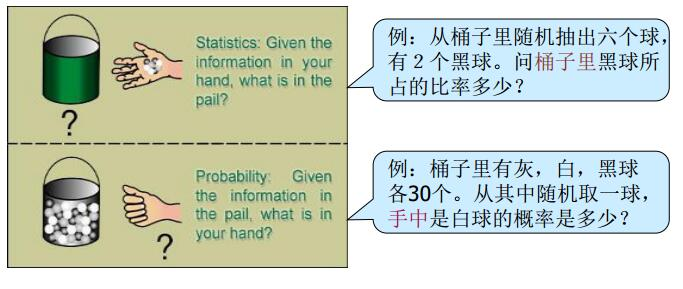
\includegraphics[width=0.6\linewidth,height=0.3\textheight]{fig/fig1}

也就是说,概率论是------我知道箱子里面是什么样的,我想知道我拿在手里的球是什么样的可能性分别有多大。统计学则是------我不知道箱子里面是什么样的,但是我已经知道我拿在手里的球是什么样的,我想靠我手里的球的样子去推断箱子是什么样的。有兴趣的也可以查看知乎上的回答。

\begin{quote}
\begin{itemize}
\tightlist
\item
  \url{https://www.zhihu.com/question/20269390}
\end{itemize}
\end{quote}

总结起来,统计学的研究过程就像下面的流程图。

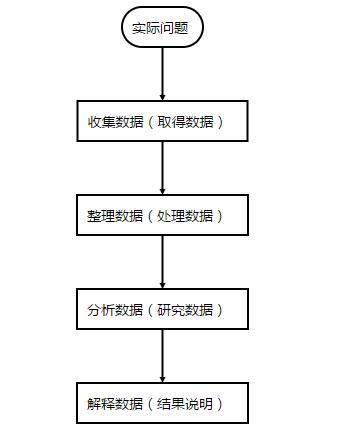
\includegraphics[width=0.8\linewidth,height=0.6\textheight]{fig/fig2}

当然这里面很容易出问题的是解释数据------数学上有意义,并不代表现实中有意义,非常容易出现很多的悖论。比如太阳升起的时间与每个人起床时间相关性很高,但是我不能说因为每个人都起床了,所以太阳升起了。

\hypertarget{ux7edfux8ba1ux65b9ux6cd5ux53caux5176ux5e94ux7528ux9886ux57df}{%
\section{统计方法及其应用领域}\label{ux7edfux8ba1ux65b9ux6cd5ux53caux5176ux5e94ux7528ux9886ux57df}}

从前面提到的我们知道,统计方法是通过已知的观测数据去分析随机现象的数量规律。因此统计方法就包括了两大部分:描述统计与推断统计。其实核心就在于我们所观测的样本是否等于总体。样本=总体,那么使用描述统计就能够用来描述我们所研究的现象。样本≠总体,那么使用推断统计才能较为准确地描述我们所研究的现象。事实上,近年来火热的大数据就是因为技术(传感器等)发展,我们足够获取可以近似等于全样本甚至全样本的数据而不是以往的样本数据所引起的一场变革,也就是说是由数据驱动的变革。

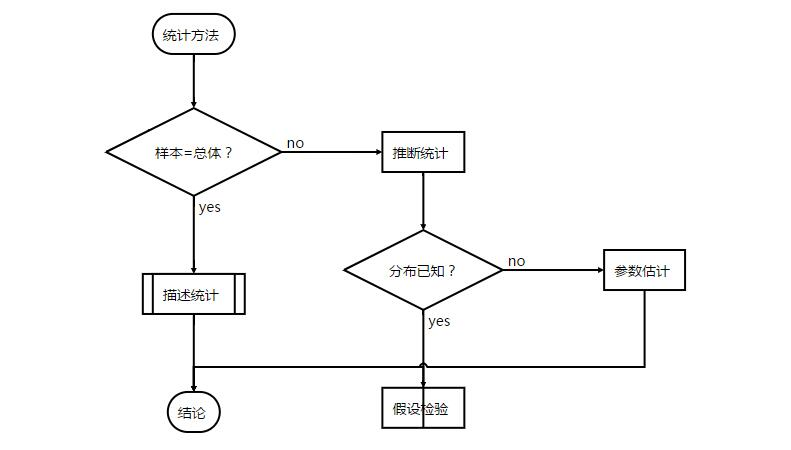
\includegraphics[width=1\linewidth,height=0.45\textheight]{fig/fig3}

统计学应用领域十分广泛,这里就不细谈了。

\hypertarget{ux7edfux8ba1ux6570ux636eux7c7bux578b}{%
\section{统计数据类型}\label{ux7edfux8ba1ux6570ux636eux7c7bux578b}}

由于应用广泛,所以统计数据类型也是多样化的。不同的划分标准类型也不相同:

(1)按照计量层次划分

\begin{quote}
\begin{itemize}
\tightlist
\item
  分类数据
\item
  顺序数据
\item
  数值数据
\end{itemize}
\end{quote}

(2)按收集方法划分

\begin{quote}
\begin{itemize}
\tightlist
\item
  调查观察数据
\item
  试验数据
\end{itemize}
\end{quote}

(3)按时间状况划分

\begin{quote}
\begin{itemize}
\tightlist
\item
  截面数据
\item
  时序数据
\end{itemize}
\end{quote}

\hypertarget{ux7edfux8ba1ux5b66ux4e2dux7684ux51e0ux4e2aux57faux672cux6982ux5ff5}{%
\section{统计学中的几个基本概念}\label{ux7edfux8ba1ux5b66ux4e2dux7684ux51e0ux4e2aux57faux672cux6982ux5ff5}}

统计学中的基本概念分别是:

\begin{quote}
\begin{itemize}
\tightlist
\item
  总体(population)------研究对象的全体
\item
  样本(sample)------研究对象的部分个体,观测数据
\item
  参数(parameter)------用来描述总体的数学度量
\item
  统计量(statistic)------用来描述样本的数学度量
\item
  变量(variable)------描述现象的某种特征
\end{itemize}
\end{quote}


\includegraphics[width=0.6\linewidth,height=0.2\textheight]{fig/fig4}

\hypertarget{datacollec}{%
\chapter{Data Collection}\label{datacollec}}

本篇是第二章,内容是数据收集。

\hypertarget{ux6570ux636eux6765ux6e90}{%
\section{数据来源}\label{ux6570ux636eux6765ux6e90}}

做科学研究离不开数据,而数据的来源有哪些呢?这里比较简单地将数据来源分为两类:直接(一手)数据和间接(二手)数据。直接数据的数据获取来源包括:观测、调查、实验。间接数据的数据获取来源包括:出版物、互联网等。

接下来分别谈谈这几个来源。观测------自然科学里有观测,如气象气候、植物生长期等,社会科学同样有观测,譬如像街区人的观测等。观测的数据可以说是纯粹第一手数据,在研究中是很宝贵的数据,但是很容易受到观测记录员主观因素的影响。调查------自然科学里的调查(室外样品采集,环境状况调查)一般是跟室内实验相结合,而社会科学的调查会更丰富,如典型的问卷调查、访谈、座谈会等。实验------实验是自然科学的核心,这里就不详述了(比如:土壤理化性质分析、植物生态生理特性分析)。不过近年来随着学科交叉增多,社会科学也开始更多地引入实验的方法(以笔者另一门公选课《初级社会网络》为例,耶鲁大学的社会心理学家米尔格兰姆(Stanley Milgram)就设计了一个连锁信件实验,这就是著名的六度分割理论的由来)。
当然除了以上三种,我认为在现在的大数据时代,还存在一些新的直接数据来源。

\begin{quote}
\begin{itemize}
\tightlist
\item
  物联网(Interest of Thing,IOT),以各类传感器(RFID、红外感应系统、GPS、通量塔等)为代表,代表数据就是如今火热的大数据------如RFID记录数据、浮动车与出租车GPS轨迹数据、通量塔测量的NEE等。
\item
  遥感(Remote Sensing,RS),某种程度上,遥感也是靠传感器接收数据,但是它与物联网还是有所差别,故单列出来。作为地学和生态学背景(尤其是GIS和RS相关方向的)的学生,对遥感会非常熟悉。遥感的特征就是,可以大范围快速获取地表信息数据(譬如地形、地表温度、气溶胶、albedo等,当然这些都需要进行反演等)。
\end{itemize}
\end{quote}

总的来说,观测在自然科学和社会科学中都有渗透较多,但是观测往往受到记录人员主观因素影响导致误差。而且观测的数据结构一般来说呈现非结构化的特征。调查在社会科学中有较多应用,自然科学中较少,而实验则是在自然科学中应用广泛,社会科学则应用较少。这两类的实质是类似的,需要提前设计好调查的大纲或者实验方案,然后按照设计好的大纲和方案进行调查和实验。也因此这两类数据结构化特征比较明显。

所谓的间接数据就是指已经经过他人整理的相关数据。这边列出来的主要包括:出版物:统计年鉴、书籍、论文等。统计年鉴是大部分社会科学相关研究的重要数据来源,这边就不详述了。书籍对于很多如社会研究的文本分析是重要的数据来源。论文作为数据,是近年来兴起的文献计量学的典型数据。此外对Meta分析,论文里的数据则是重要来源。互联网:百度指数、阿里指数、大众点评等数据。互联网数据可以利用网络爬虫获取。总的来说,间接数据易于获取,作用广泛,但使用的时候需要控制数据质量以及引用。

\hypertarget{ux8c03ux67e5ux8bbeux8ba1}{%
\section{调查设计}\label{ux8c03ux67e5ux8bbeux8ba1}}

这边主要介绍的是数据的调查方式、调查方案的结构和设计以及调查问卷设计。

(1)数据的调查方式

数据的调查方式一般而言是遵循统计学规律的(我们称之为统计调查方式),这里列举了我国统计调查的常用方式:普查(人口普查、农业普查、甚至到最近刚刚发布成果的全国第一次地理国情普查)、抽样调查(概率抽样、非概率抽样,具体后面第三章会详述)、统计报表(统计公报)。而除了以上之外,当我们需要自己收集直接数据的时候又可以分为以下几种:

询问调查类:

\begin{quote}
\begin{itemize}
\tightlist
\item
  访问调查
\item
  邮寄调查
\item
  电话调查
\item
  电脑辅助
\item
  座谈会
\item
  个别深访
\end{itemize}
\end{quote}

观察实验:

\begin{quote}
\begin{itemize}
\tightlist
\item
  观察
\item
  实验
\end{itemize}
\end{quote}

(2)调查方案的结构和设计

如何做调查?是很多人在科学研究中的第一道难关。这里给出一个关于做调查的普遍步骤流程图:

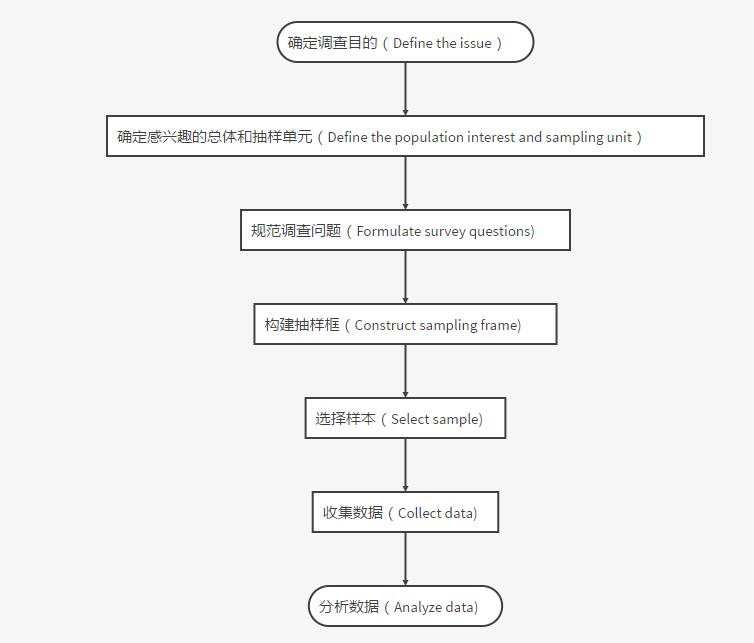
\includegraphics[width=1\linewidth,height=0.6\textheight]{fig/fig5}

那么调查方案又是什么呢?我认为调查方案就是调查的策划书。明确你调查的一些目的、对象、项目以及调查方法等。一般结构如下:

\begin{quote}
\begin{itemize}
\tightlist
\item
  调查目的
\item
  调查对象调查单位
\item
  调查项目
\item
  其他
\end{itemize}
\end{quote}

(3)调查问卷设计

最后这部分是谈谈调查问卷设计的一些内容(包括笔者自己的一些经验)。

问卷结构

\begin{quote}
\begin{itemize}
\tightlist
\item
  开头部分(问候语、填写说明、问卷编号 )
\item
  甄别部分
\item
  主体部分
\item
  背景部分
\end{itemize}
\end{quote}

其他部分就不详述了,甄别部分一般是针对过滤的问题,就是不符合条件的即可跳过部分调查题目。接下来主要针对主体部分简单介绍。主体部分其实就是问卷主要调查的部分。一般来说要注意一下几点。

\begin{quote}
\begin{itemize}
\tightlist
\item
  提问内容尽可能简短
\item
  用词准确通俗(可按6W原则推敲:Who,Where,When,Why,What,How)
\item
  一项提问只包括一项内容
\item
  避免诱导性提问、否定形式提问、敏感性问题
\end{itemize}
\end{quote}

而问题则又可以分为两大类:开放性问题(自由回答型)和封闭性问题(选择回答型)。封闭性问题包括了二项选择、多项选择(单项、多项、限制选择)、顺序选择法、评定尺度法、双向列联表法。

\begin{quote}
\begin{itemize}
\tightlist
\item
  开放性问题------一般就是可以随便答,这类数据一般是问卷者的主观感受,不会受客观影响。但是最大的问题在于数据收集呈现非结构化特征,多以文本形式存在。研究时必须通过重编码、文本分析等方法。
\item
  封闭性问题------相当于是选择题或者填空题。二项选择就是,只有两个选项(A或B);多项选择则是有多个选项,可以选至少一个(一个为单项、一个以上且不限制选择的数量为多项、一个以上且限制选择的数量为限制);顺序选择法,就是给出多个选项,让你按照自己的认识对选项进行排序;评定尺度法,给出多个选项且是有等级划分的(如很差,差,一般,好,很好)进行选择;双向列联表法,将两类不同问题综合到一起,用表格形式,横向为一类问题,纵向为一类问题。
\end{itemize}
\end{quote}

从笔者的经验来说,在设置问卷的时候,必须要先从自己想研究的问题出发,思索如何用数据分析证明自己的结论,然后大致思索需要用来分析的统计方法与统计指标,然后对应选择问题的形式,因为不同的问题形式对应的数据结构大不相同,而且统计方法也不尽相同。最后的最后安利大家一个软件:Survey123 for ArcGIS。这是由esri北京研发中心开发的一款外业数据收集软件------获得``问卷好帮手''称号的application。

\begin{quote}
\begin{itemize}
\tightlist
\item
  \url{http://www.esri.com/products/survey123}
\end{itemize}
\end{quote}

主要包括了桌面端Survey123 connect和移动端Survey123 app两大软件。可以简便地建立问卷、分享问卷、搜集数据、分析数据,同时采集时受访者的GPS位置也将被记录。具体教程参照如下网址。

\begin{quote}
\begin{itemize}
\tightlist
\item
  \url{http://doc.arcgis.com/zh-cn/survey123/}
\end{itemize}
\end{quote}

\hypertarget{ux6570ux636eux8d28ux91cf}{%
\section{数据质量}\label{ux6570ux636eux8d28ux91cf}}

采集数据的时候必须考虑的就是数据的质量,即降低采集数据时产生误差。科学研究中的数据误差无可避免,而误差的来源主要包括:抽样误差、非抽样误差。抽样误差,在抽样方式确定时就无法避免,具体的方法可能还是统计学万能解药---------增加样本量。非抽样误差则包括了如下的内容:

\begin{quote}
\begin{itemize}
\tightlist
\item
  抽样框误差
\item
  回答误差
\item
  无回答误差
\item
  调查员误差
\end{itemize}
\end{quote}

抽样框误差------其实就是抽取的样本无法代表总体;回答误差和无回答误差都是由于受访者导致的错误,而调查员误差则无须再介绍,即采集者自身的误差。那么控制误差的方法无非就在于样本大小以及合适的数据框(针对非抽样误差和抽样框误差),靠重访来进行修正(回答误差和无回答误差),调查员误差则需要对调查员进行培训。当然这里还得普及一个概念,在统计学里面,precision(精度)和accuracy(准确性)是不相同的。中文里面往往因为两个单词都翻译成精度,事实上这两个词指的是不一样的内容。二者的区别可以看下面的图。

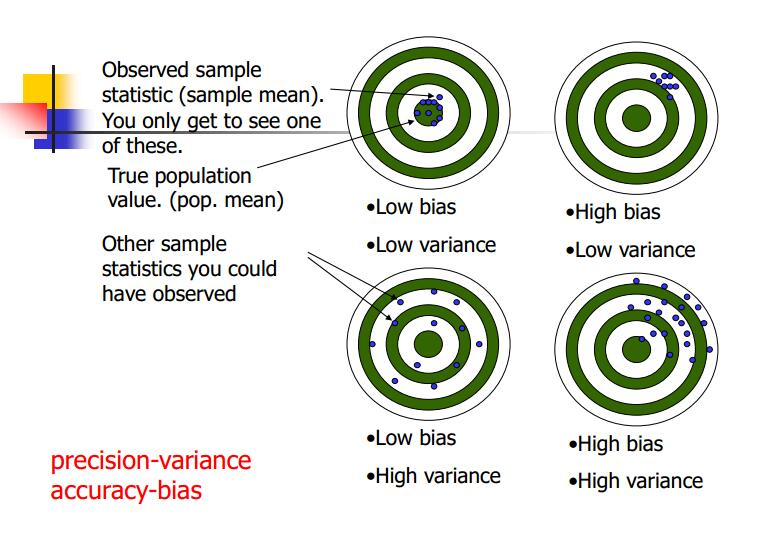
\includegraphics[width=1\linewidth,height=0.5\textheight]{fig/fig6}

\hypertarget{descriptive}{%
\chapter{Descriptive Statistics}\label{descriptive}}

本篇是第三章,内容是描述性统计。同时在这一章会开始渗透R语言的相关内容。但整体还是以理论为主。

\hypertarget{ux6570ux636eux7684ux9884ux5904ux7406}{%
\section{数据的预处理}\label{ux6570ux636eux7684ux9884ux5904ux7406}}

本章正式进入统计学的一大分支------描述统计。很多人会疑惑做一个Project或者写一篇Paper,最难的是什么?我曾经不止一次说过,最难的是数据。数据收集完成,项目完成了50\%。而数据收集完成之后,很多人就会马上开始进行数据处理和分析,事实上这是不对的。因为你不清楚你的数据是否有问题(什么问题都有可能,会导致你的分析出现各种问题)。所以你拿到数据后的第一步,应该是对数据做预处理,或者用大数据时代的话------叫数据清洗或者ETL(Extract-Transform-Load),我想预处理还会占掉Project花费时间的20\%吧。

那么接下来先介绍下预处理的内容。

数据预处理:

\begin{quote}
\begin{itemize}
\tightlist
\item
  数据审核
\item
  数据筛选
\item
  数据排序
\item
  数据透视
\end{itemize}
\end{quote}

数据审核,包括直接数据的完整性审核以及准确性审核(是否客观),间接数据的适用性审核以及时效性审核;数据筛选,就是对于数据里面的异常值(存在错误,不符合调查要求等),在现在来说就是dirty data(脏数据),将这些数据剔除;数据排序,事实上数据排序更多的目的还是为了更方便地发现异常值,是做数据清洗的手段;数据透视,借鉴于Excel里的数据透视表,事实上就是数据的重铸,融合和汇总,从而得到我们需要的数据。

总的来说,前期预处理需要对数据进行排序、汇总和观察发现相关的数据异常值等。在这个阶段,不喜编程的同学推荐用Excel来做数据预处理(通过数据透视图、替换数据、排序、Countif等工具和Excel函数高效完成预处理),更高级的一般可以考虑用R、Python等编程语言进行清洗预处理,或者像在数据库里用SQL语句也是可以的。

响应一下本部分的标题,R语言实现,交代几个简单的语句进行数据清洗。

\begin{Shaded}
\begin{Highlighting}[]
\CommentTok{#x为数据框、数组或矩阵}
\CommentTok{#通过summary可以获取平均值、中位数、四分位数等,如果有缺失数据,则会显示NAN等。}
\KeywordTok{summary}\NormalTok{(x)}
\CommentTok{#表示y是按照x的第一行先升序排列,然后再按x的第二列降序排列得到的数据,-表示降序。}
\NormalTok{y <-}\StringTok{ }\NormalTok{x[}\KeywordTok{order}\NormalTok{(x[}\DecValTok{1}\NormalTok{], }\OperatorTok{-}\NormalTok{x[}\DecValTok{2}\NormalTok{])}
\CommentTok{#去除NA所在行和列}
\NormalTok{y <-}\StringTok{ }\KeywordTok{na.omit}\NormalTok{(x)}
\end{Highlighting}
\end{Shaded}

\hypertarget{ux6570ux636eux7684ux6574ux7406ux4e0eux5c55ux793a}{%
\section{数据的整理与展示}\label{ux6570ux636eux7684ux6574ux7406ux4e0eux5c55ux793a}}

这部分的数据整理是在预处理完毕后,根据我们需要对数据进行整理和简单可视化(多画图,多可视化,你能发现很多事情)。那么第一步就是先把我们的数据类型搞清楚。因为不同类型数据,整理方式不同。对于分类数据和顺序数据主要是分类整理。对于数值数据主要是做分组整理。

\begin{quote}
\begin{itemize}
\tightlist
\item
  分类数据的整理核心就是计算频数、比例、百分比、比率,一般可视化用条形图(柱状图)。此外还可以考虑使用帕累托图。帕累托图(Pareto chart)是以意大利经济学家V.Pareto的名字而命名的。这是一个双坐标轴图,一侧纵坐标是频率,另一侧纵坐标是累计频率。是在条形图基础上加上一条折线图(累计频率曲线)。通常用帕累托图来表示,就是研究事物特征是否存在二八定律(20/80规律,典型案例:20\%的人拥有80\%的财富)。除此之外,分类型数据还可以用饼图来进行可视化。
\item
  顺序数据则一般选用累计频率曲线和环状图进行可视化。
\item
  数值型数据的可视化方式是最多的。主要包括了直方图、折线图(频数多边形图)、打点图、茎叶图、箱线图、线图(时间序列数据)、双变量问题(二维散点图与散点图矩阵)、三变量问题(三维散点图或气泡图)、多变量问题(雷达图)。
\end{itemize}
\end{quote}

其中这里面有一个直方图分组使用的经验公式。

\[K=1+\frac{\lg {n}}{\lg {2}}\],

K为组数,n为样本数。确定组数,通过极差和组数求组距即可分组。

这部分有很多可视化内容,暂时就不在这部分讲述了(第14章会重点讲解几个典型的可视化方式的R语言绘制)。最后小结下数据可视化的内容。

\begin{quote}
\begin{itemize}
\tightlist
\item
  品质数据------先制作汇总表,然后可以采用条形图、饼图、环状图可视化;
\item
  数值数据中的原始数据------茎叶图、箱线图可视化;
\item
  数值数据中的分组数据------直方图、折线图;
\item
  数值数据中的时间序列数据------线图;
\item
  数值数据中的多元数据------散点图、气泡图、雷达图。
\end{itemize}
\end{quote}

此外对于图表可视化来说,好的图表可视化应当具有如下特征:

\begin{quote}
\begin{itemize}
\tightlist
\item
  显示数据;
\item
  让读者把注意力集中在图表的内容上,而不是制作图表的程序上;
\item
  强调数据之间的比较;
\item
  服务于一个明确的目的;
\item
  有对图表的统计描述和文字说明。
\end{itemize}
\end{quote}

鉴别图表优劣的准则:

\begin{quote}
\begin{itemize}
\tightlist
\item
  精心设计、 有助于洞察问题的实质;
\item
  使复杂的观点得到简明、 确切、 高效的阐述;
\item
  能在最短的时间内以最少的笔墨给读者提供最大量的信息;
\item
  表述数据的真实情况, 避免歪曲。
\end{itemize}
\end{quote}

当然图表可视化不仅仅只有R,Excel、SPSS、Tableau都可以使用。

\hypertarget{ux6570ux636eux7684ux6982ux62ecux6027ux5ea6ux91cf}{%
\section{数据的概括性度量}\label{ux6570ux636eux7684ux6982ux62ecux6027ux5ea6ux91cf}}

当你面对一堆数据时,你还是不知道从何下手,因为我们不可能强行记住每个数据,然后在脑海里对各个数据的分布进行比较,所以科学家们在处理数据的时候,都希望用数据规模尽可能小的一个指标去描述数据尽可能多的信息。那么从数据的角度出发,针对数据分布的不同方面,科学家们也都找出了不相同的指标来进行描述。

简单来说,数据分布包括了集中趋势、离散程度、分布形状三个方面的内容。

\begin{quote}
\begin{itemize}
\tightlist
\item
  集中趋势:众数、中位数、平均数;
\item
  离散程度:异众比率、四分位差、极差、方差或标准差、离散系数;
\item
  分布形状:偏态系数、峰态系数。
\end{itemize}
\end{quote}

集中趋势的几个指标想必大家较为清楚,就不展开详述了。而离散程度中极差、方差和标准差也是如此,同上,不过单独解释下自由度的概念(一组数据中可以自由取值的数据的个数,与附加给独立观测值的约束或限制的个数有关,比如三个数据的均值已经知道,知道其中两个数据,第三个数据是固定的,也就是说在添加了均值这个约束之后,观测数据自由取值的个数是n-1=2个)。这里重点解释异众比率,四分位差、离散系数、偏态系数和峰态系数。

\begin{quote}
\begin{itemize}
\tightlist
\item
  异众比率------从字面理解即可,非众数的比率。也就是------不是众数的组的频数占总频数的比率。
\item
  四分位差------上四分位数减去下四分位数。
\item
  离散系数------也就是标准差系数,即用标准差除以平均值。
\item
  偏态系数------用来描述数据分布特征(分布偏斜程度)的系数,该系数\textgreater0为右偏分布,\textless0为左偏分布,=0为对称分布。
\item
  峰态系数------用来描述数据分布特征(分布扁平程度)的系数,该系数\textgreater0为尖峰分布,\textless0为扁平分布,=0为扁平峰度适中。
\end{itemize}
\end{quote}

最后单列出以上部分指标的公式(有数学恐惧症的同学请跳过)。

中位数:

\[x_{((n+1)/2)}\](n为奇数)

\[(x_{(n/2)}+x_{(n/2)+1})/2\](n为偶数)

四分位数:

\[Q_{L}=\frac{n}{4},Q_{U}=\frac{3n}{4}\]

\[Q_{L}=\frac{n+1}{4},Q_{U}=\frac{3(n+1)}{4}\]

\[Q=\frac{[\frac{n+1}{2}]+1}{2}\]

\[Q_{L}=\frac{n+3}{4},Q_{U}=\frac{3n+1}{4}\]

平均数:

\[\bar{x}=\frac{\sum_{i=1}^n x_{i}}{n}\](简单平均数)

\[\bar{x}=\frac{\sum_{i=1}^k M_{i}f_{i}}{n}\](加权平均数)

\[G_{m}=\sqrt[n] {\prod_{i=1}^n {(1+x_{i})}}-1\](几何平均数)

异众比率:

\[v_r=1-\frac{f_m}{\sum f_i}\]

极差:

\[R=max(x_i)-min(x_i)\]

四分位差:

\[Q_d=Q_U-Q_L\]

平均差:

\[M_d=\frac{\sum_{i=1}^n \left|{x_i-\bar {x}}\right|}{n} \] 或 \[ M_d=\frac{\sum_{i=1}^k \left|{M_i-\bar {x}}\right|f_i}{n}\]

总体方差:

\[\sigma^2=\frac{\sum_{i=1}^N (x_i-\mu)^2}{n} \] 或 \[ \sigma^2=\frac{\sum_{i=1}^k (M_i-\mu)^2f_i}{n}\]

总体标准差:

\[\sigma=\sqrt {\frac{\sum_{i=1}^N (x_i-\mu)^2}{n}} \] 或 \[ \sigma=\sqrt{\frac{\sum_{i=1}^k (M_i-\mu)^2f_i}{n}}\]

样本方差:

\[s^2=\frac{\sum_{i=1}^N (x_i-\bar x)^2}{n-1} \] 或 \[ s^2=\frac{\sum_{i=1}^k (M_i-\bar x)^2f_i}{n-1}\]

样本标准差:

\[s=\sqrt {\frac{\sum_{i=1}^N (x_i-\bar x)^2}{n-1}} \] 或 \[ s=\sqrt{\frac{\sum_{i=1}^k (M_i-\bar x)^2f_i}{n-1}}\]

标准分数:

\[z_i=\frac{x_i-\bar{x}}{s}\]

标准差系数:

\[v_s=\frac{s}{\bar{x}}\]

偏态系数:

\[SK=\frac{n\sum(x_i-\bar{x})^3}{(n-1)(n-2)s^3}\]

\[SK=\frac{\sum_{i=1}^k(M_i-\bar{x})^3f_i}{ns^3}\]

峰态系数:

\[K=\frac{n(n+1)\sum{(x_i-\bar{x})^4}-3[\sum{(x_i-\bar{x})^2}]^2(n-1)}{(n-1)(n-2)(n-3)s^4}\]

\[K=\frac{\sum_{i=1}^k{(M_i-\bar{x})^4f_i}}{ns^4}-3\]

\hypertarget{sampling}{%
\chapter{Sampling And Sample Distribution}\label{sampling}}

本篇是第四章,内容主要是抽样方法与抽样分布。这一章内容比较多(从抽样方法一直到许多分布函数,尤其是介绍了四个重要分布------正态分布、卡方分布、t分布、F分布,以及部分统计推断的内容)。

\hypertarget{ux62bdux6837ux65b9ux6cd5}{%
\section{抽样方法}\label{ux62bdux6837ux65b9ux6cd5}}

抽样调查的概念前面已经有所涉及到,这里就不详述了。大部分情况下,普查是不太可能的,所以抽样调查是科学研究中应用最为广泛的收集数据的方法。但是正如前面在谈论precision和accuracy问题的时候说的,我们希望数据的质量是Low Bias and Low Variance,抽样调查的样本既能很好地代表总体(非抽样误差小),同时多次抽样的话,也希望抽样的样本大致都接近,降低抽样误差。所以从统计学诞生至今,已经提出了很多的抽样方法。可以说并没有任何一种方法能完全避免这些误差,这些方法需要根据具体情境具体使用。

总的来说,抽样方法可以分为两大类:概率抽样与非概率抽样。概率抽样是根据一个已知的概率来抽取样本单位(也称为随机抽样),概率抽样要求按照一定的概率随机抽取样本,也就是说每个样本都有一定的机会被抽中,同时每个样本被抽中的概率是可以已知或计算出来的,而当运用概率抽样的样本进行参数估计的时候必须考虑样本被抽中的概率(某种程度来说感觉类似贝叶斯,先验概率和后验概率的问题)。概率抽样包括了:

\begin{quote}
\begin{itemize}
\tightlist
\item
  简单随机抽样------从总体N个单位里抽出n个单位作为样本(可以重复抽样,也可以不重复抽样),最常用的抽样方式,参数估计和假设检验主要依据的就是简单随机样本。
\item
  系统抽样------将总体中的所有单位(抽样单位)按一定顺序排列, 在规定的范围内随机地抽取一个单位作为初始单位, 然后按事先规定好的规则确定其他样本单位(先从数字1到k之间随机抽取一个数字r作为初始单位,以后依次取r+k, r+2k\ldots 等单位)。
\item
  分层抽样------将总体单位按某种特征或某种规则划分为不同的层(Strata), 然后从不同的层中独立、 随机地抽取样本。
\item
  整群抽样------将总体中若干个单位合并为组(群), 抽样时直接抽取群, 然后对中选群中的所有单位全部实施调查。
\item
  多阶段抽样------先抽取群, 但并不是调查群内的所有单位, 而是再进行一步抽样,从选中的群中抽取出若干个单位进行调查(群是初级抽样单位,第二阶段抽取的是最终抽样单位。将该方法推广, 使抽样的段数增多, 就称为多阶段抽样)
\end{itemize}
\end{quote}

非概率抽样则不是按照随机的原则选取样本,而是根据研究的具体需求选取调查样本。非概率抽样包括了:

\begin{quote}
\begin{itemize}
\tightlist
\item
  方便抽样------研究员依据方便的原则选取对应的样本。
\item
  判断抽样------研究员根据自己的判断选择样本。
\item
  自愿样本------被调查者自愿参加调查提供信息。举个跟地学相关的例子------志愿地理信息(Volunteer Geographcial Information,VGI),是指利用工具创建、组装和传播个人资源提供的地理数据,像社交媒体中的签到。
\item
  滚雪球抽样------首先选择一组进行调查,让调查者提供另外一些属于调查总体的调查对象,然后持续下去
\item
  配额抽样------先将体中的所有单位按一定的标志(变量) 分为若干类, 然后在每个类中采用方便抽样或判断抽样的方式选取样本单位。
\end{itemize}
\end{quote}

总的来说,各种抽样方式各有各有的优缺点,根据研究具体情况进行选择。而实际研究中简单随机抽样的应用更多些,这边提供R语言中做简单随机抽样的代码示例。

\begin{Shaded}
\begin{Highlighting}[]
\CommentTok{#N表示总体的数据,n为抽样单位,replace=FALSE代表不重复抽样,replace=TRUE代表重复抽样}
\NormalTok{n <-}\StringTok{ }\KeywordTok{sample}\NormalTok{(N,n,}\DataTypeTok{replace =} \OtherTok{FALSE}\NormalTok{)}
\end{Highlighting}
\end{Shaded}

\hypertarget{ux6b63ux6001ux5206ux5e03}{%
\section{正态分布}\label{ux6b63ux6001ux5206ux5e03}}

正态分布由高斯作为描述误差相对频数分布的模型而提出的:

\begin{quote}
\begin{itemize}
\tightlist
\item
  描述连续型随机变量的最重要的分布
\item
  许多现象都可以由正态分布来描述
\item
  可用于近似离散型随机变量的分布
\item
  经典统计推断的基础
\end{itemize}
\end{quote}

正态分布的意义,多多少少大家都有了解,这里就不再详述了。随机变量服从\(X\sim N (\mu,\sigma^2)\),则X的概率密度函数为

\[f(x)=\frac{1}{\sigma\sqrt{2\pi}}e^{-\frac{1}{2}(\frac{x-\mu}{\sigma})^2} -\infty<x<\infty\]

这就是正态分布的概率密度函数。正态分布具有如下性质:

\begin{quote}
\begin{itemize}
\tightlist
\item
  关于x=\(\mu\)的钟形对称性质,峰值在x=\(\mu\)处。
\item
  均值和标准差一旦决定,该分布形式也就决定了。
\item
  均值决定分布函数位置,标准差决定函数的扁平程度。
\item
  X轴两侧无限延伸,f(x)无限逼近x轴,但理论上不可能相交。
\item
  正态随机变量在特定区间上的取值概率由正态曲线下的面积给出,而且其曲线下的总面积等于1
\end{itemize}
\end{quote}

下图给出了两个图(一个是用核密度生成的曲线,一个是正态分布概率密度函数)来说明以上的部分性质(具体实现的R语言代码在附录文件夹中的src里面)。

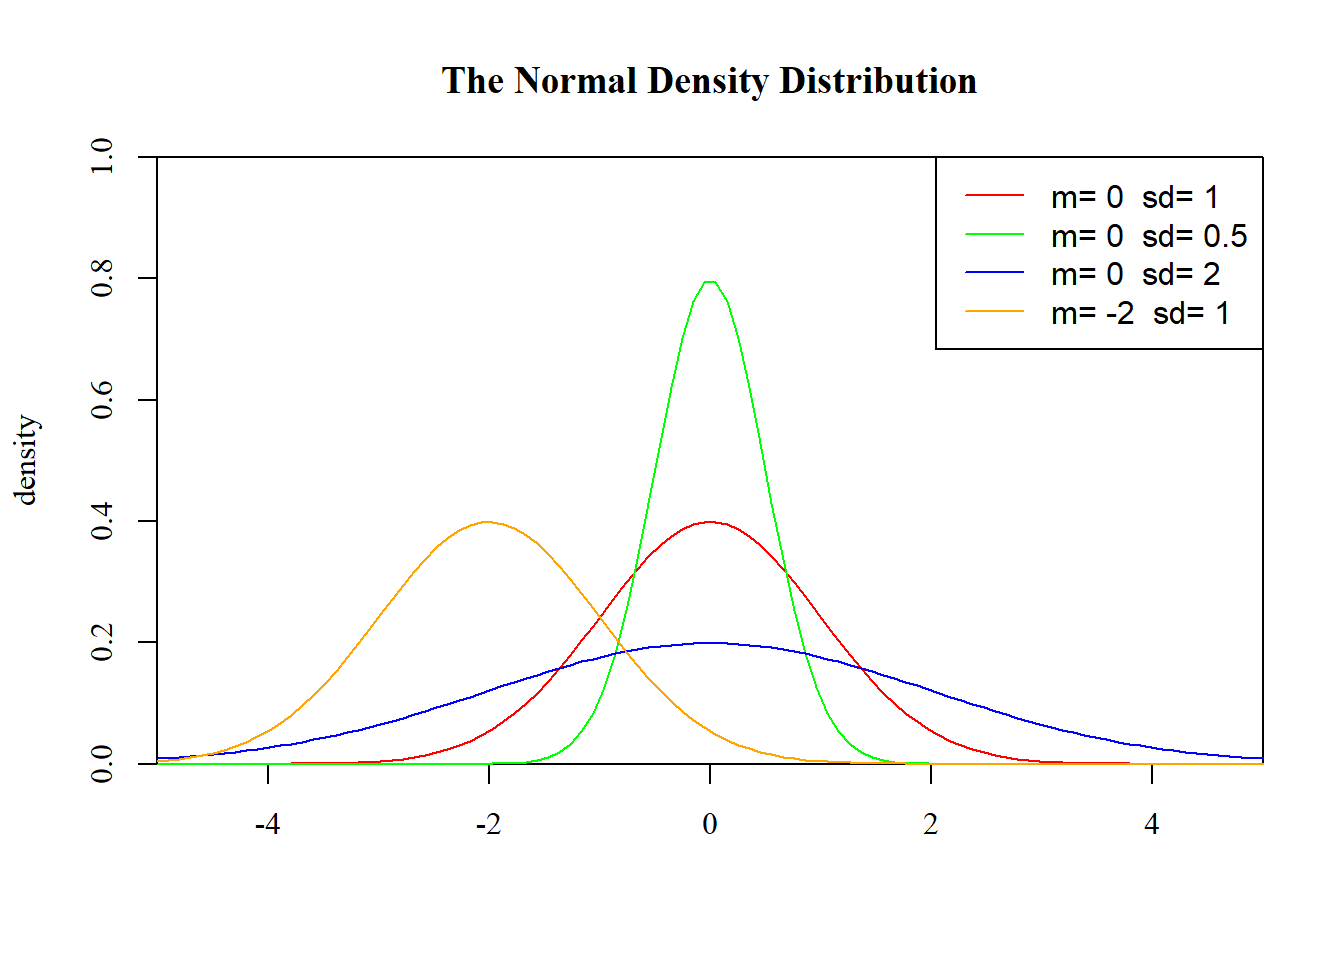
\includegraphics[width=1\linewidth,height=0.4\textheight]{bookdown_files/figure-latex/unnamed-chunk-9-1}

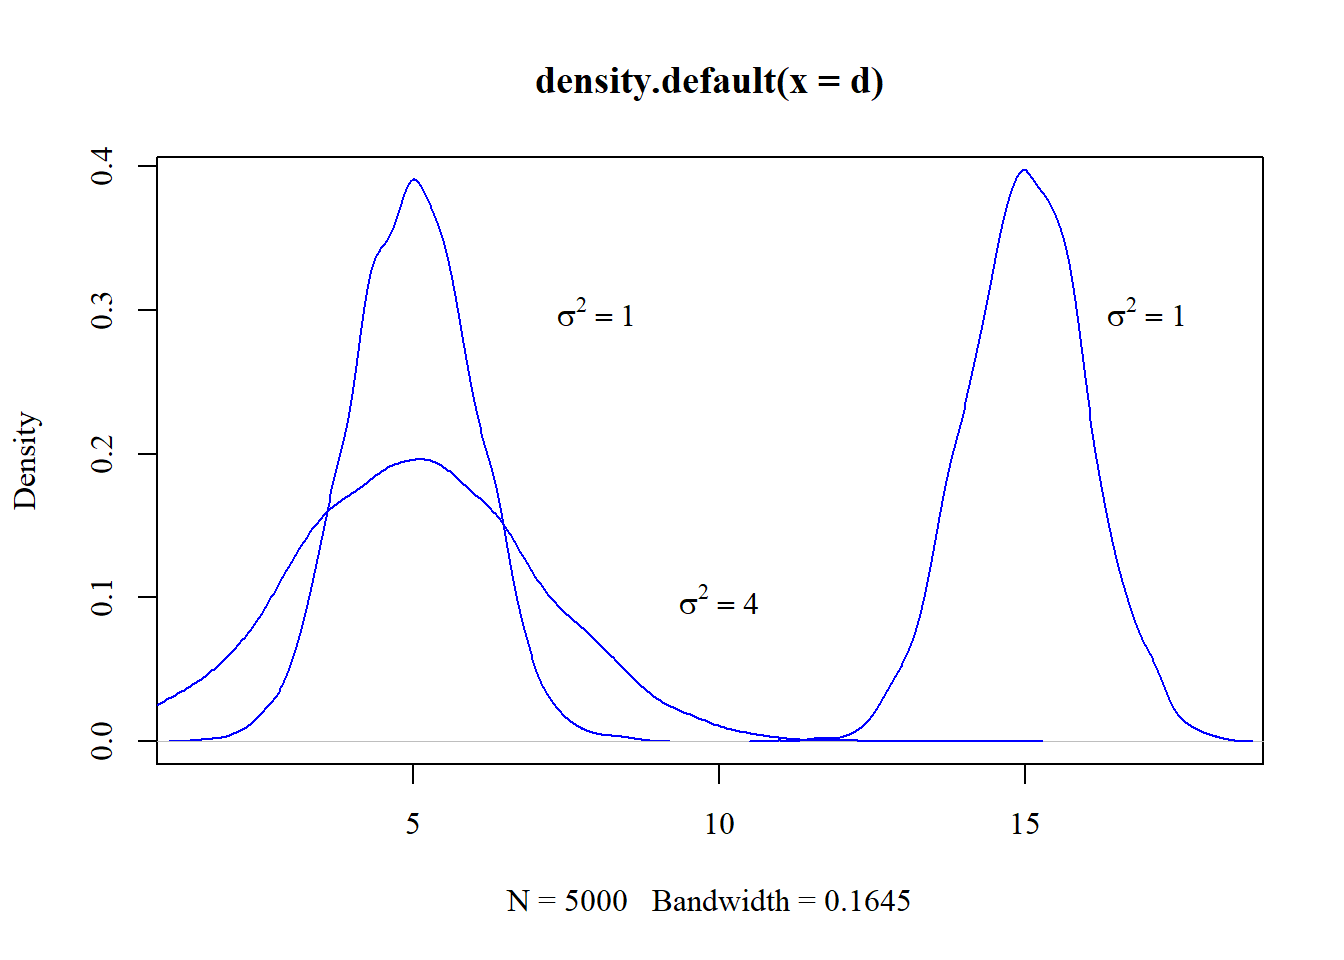
\includegraphics[width=1\linewidth,height=0.4\textheight]{bookdown_files/figure-latex/unnamed-chunk-10-1}

标准正态分布就是指均值为0,标准差为1的正态分布。通过标准正态分布可以很方便地求算各种概率,所以实际应用中,往往将正态分布数据通过标准化的方式转化为标准正态分布求解具体概率。即令\(Z=\frac{x-\mu}{\sigma}\),则Z服从标准正态分布。那么如何检验数据的正态性呢?一般有以下几种方法:

\begin{quote}
\begin{itemize}
\tightlist
\item
  对数据画出频数分布的直方图或茎叶图(若数据近似服从正态分布, 则图形的形状与上面给出的正态曲线应该相似)。
\item
  求出样本数据的四分位差和标准差, 然后二者计算比值。 若数据近似服从正态分布,则有
  \[Q_d/s\approx1/3\]
\end{itemize}
\end{quote}

\begin{quote}
\begin{itemize}
\tightlist
\item
  拟合优度检验
\end{itemize}
\end{quote}

一般可以通过画这个图来进行检验(代码同在附录文件夹src中这一章的代码文件里面)。

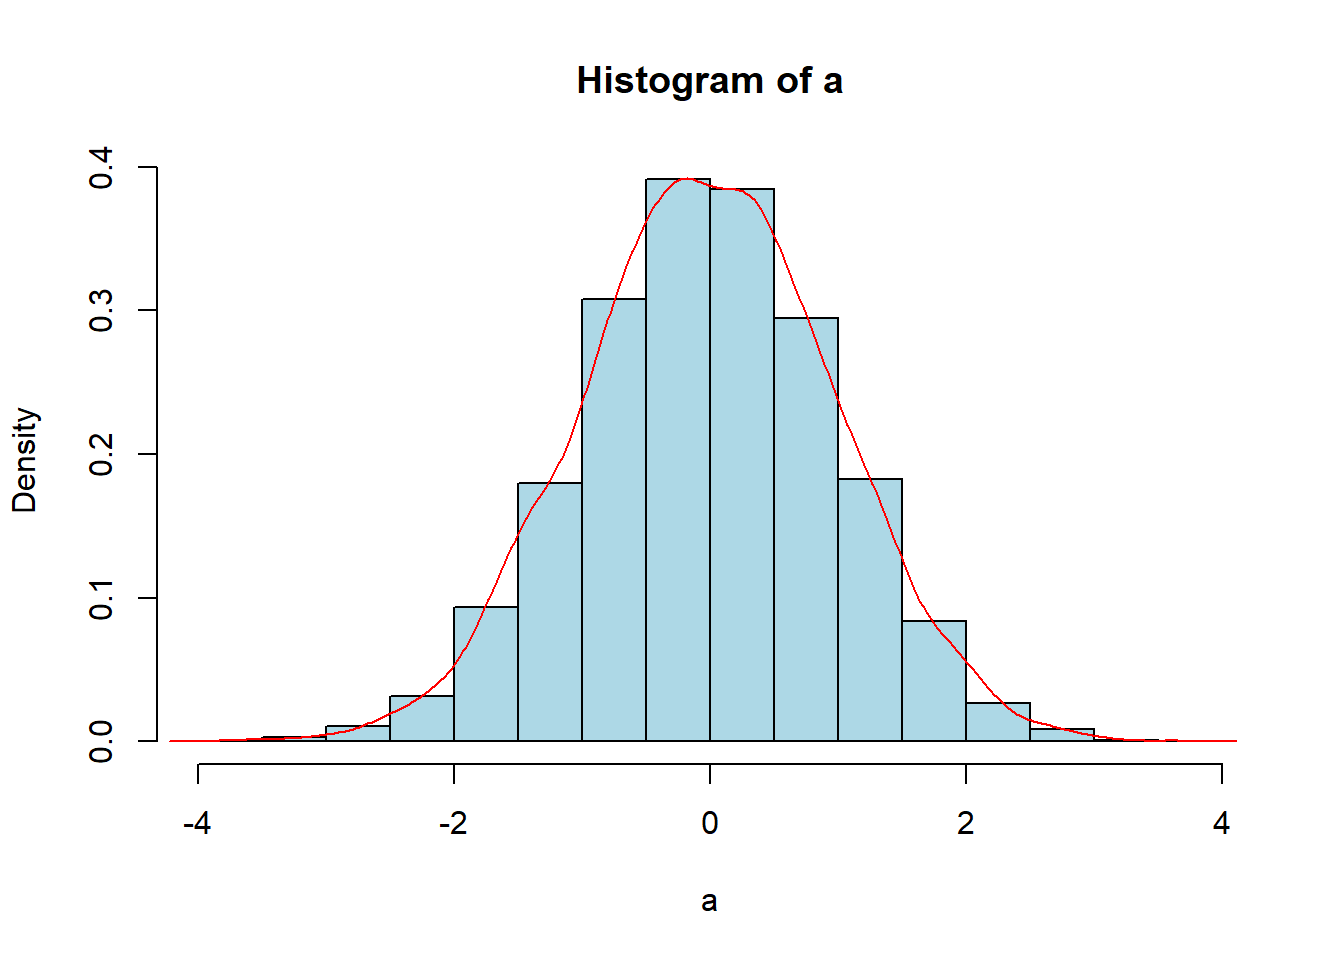
\includegraphics[width=1\linewidth,height=0.4\textheight]{bookdown_files/figure-latex/unnamed-chunk-11-1}

或者计算四分位差和标准差比值。这里给出这个方法的R语言实现(用户自编函数)。

\begin{Shaded}
\begin{Highlighting}[]
\NormalTok{Normaltestindex <-}\StringTok{ }\ControlFlowTok{function}\NormalTok{(x) \{ }
\NormalTok{  q =}\StringTok{ }\KeywordTok{fivenum}\NormalTok{(x)}
\NormalTok{  Qd =}\StringTok{ }\NormalTok{q[}\DecValTok{4}\NormalTok{] }\OperatorTok{-}\StringTok{ }\NormalTok{q[}\DecValTok{2}\NormalTok{]}
\NormalTok{  s =}\StringTok{ }\KeywordTok{sd}\NormalTok{(x)}
\NormalTok{  Normaltestindex =}\StringTok{ }\NormalTok{Qd}\OperatorTok{/}\NormalTok{s}
  \KeywordTok{cat}\NormalTok{(}\StringTok{"The Qd/s"}\NormalTok{, Normaltestindex)}
\NormalTok{\}}
\end{Highlighting}
\end{Shaded}

拟合优度检验是后面章节内容,这里不详述。正态分布在各样本相互前提下存在线性可加性。\(x_i\sim N(\mu_i,\sigma_i)\),且\(x_i\)相互独立,则
\(\Sigma a_ix_i\sim N(\Sigma a_i\mu_i,\Sigma a_i^2\sigma_i^2)\)。同时样本量够大情况下,n个独立随机变量之和服从正态分布。

\hypertarget{ux4e09ux79cdux4e0dux540cux6027ux8d28ux7684ux5206ux5e03}{%
\section{三种不同性质的分布}\label{ux4e09ux79cdux4e0dux540cux6027ux8d28ux7684ux5206ux5e03}}

统计量(statistic)------样本来自总体,必然携带有反映总体性质的各种信息。统计的基本任务就是通过对样本的研究来对总体的未知参数或分布类型作出估计,对有关总体的假设作出推断。样本是进行统计推断的依据。但在实际应用时,一般不是直接使用样本本身,而是对样本进行整理和加工, 即针对具体问题构造适当的函数---统计量, 利用这些函数来进行统计推断,揭示总体的统计特性。事实上统计量把分散在样本中的总体信息按需要集中在一个函数上,使该函数能反映总体方面的信息。

概念很拗口,总结起来就是,我懒得分析(也没法分析,因为有些总体无法穷尽)总体的分布,我就偷懒地先抽样,并且认为样本能够代表总体特征,再偷懒地计算某些指标,这些指标可以反映样本数据分布特征,这些指标就叫统计量,然后再用统计量去推出(猜)总体的分布特征(第一章提到了,应该叫参数)------果然``懒''才是人类进步的动力。

当然这里要区分两个概念------统计量与观察值。假设\(X_1,X_2, \cdots ,X_n\)是来自总体X的样本, \(x_1,x_2,\cdots ,x_n\)为其样本值, 则称不含任何总体分布中未知参数的函数\(g(X_1,X_2,\cdots,X_n)\)为统计量,相应实数\(g(x_1,x_2,\cdots,x_n)\)为观察值。如何理解这二者区别呢?其实这里把样本看成了一组随机变量,因为在未抽样前,样本观察值未知,样本就是个随机变量(所以一般来说统计推断的基础是简单随机抽样),但是抽样之后,样本就是一组确定的观察值,这也可以说是样本的二重性。常用的统计量包括了样本均值、样本方差、样本标准差、样本k阶原点矩、样本k阶中心距(具体公式的话,文末附录给出)。从前面提到的统计推断基础是简单随机抽样,也就是要求样本是简单随机样本,那么简单随机样本又是什么呢?

首先随机样本的概念:随机抽取的n个个体的集合\((X_1,X_2, \cdots ,X_n)\),n为样本容量。而简单随机样本则需要在随机样本的前提上满足以下两个条件:

\begin{quote}
\begin{itemize}
\tightlist
\item
  随机性:总体中每个个体都有同等机会被选到样本中,即\(X_i\)与X同分布
\item
  独立性:样本中每个个体的选取不影响其他个体的选取,即\(X_1,X_2, \cdots ,X_n\)是相互独立的随机变量
\end{itemize}
\end{quote}

接下来是标题提到的三种不同性质的分布:总体分布、样本分布、抽样分布。

\begin{quote}
\begin{itemize}
\tightlist
\item
  总体分布------总体中各元素的观察值所形成的分布,分布通常是未知的,可以假定它服从某种分布。
\item
  样本分布------一个样本中各观察值的分布,也称经验分布,当样本容量 n 逐渐增大时,样本分布逐
  渐接近总体的分布。
\item
  抽样分布------样本统计量的概率分布, 是一种理论分布,又称为诱导分布,在重复选取容量为n 的样本时,由该统计量的所有可能取值形成的相对频数分布,随机变量是样本统计量(样本函数,如样本均值,样本比例,样本方差等),结果来自容量相同的所有可能样本,提供了样本统计量长远而稳定的信息,是进行推断的理论基础,也是抽样推断科学性的重要依据( 点估计、 置信区间、假设推断等)。
\end{itemize}
\end{quote}

用一个简单的例子来说明三者的区别。假设总体N=4,随机变量X=年龄。总体分布如下,均值为21,方差为2.236。这里提醒用R语言做统计的同学,R语言默认的var和sd都是求样本的标准差(分母是n-1和n的差别),当你的数据是总体时,建议另外计算,或者可以使用我下面的自编函数(给了个标准差的样例,方差的可以在附录文件夹src中这一章的代码文件里面找)。

\begin{Shaded}
\begin{Highlighting}[]
\NormalTok{Populationsd <-}\StringTok{ }\ControlFlowTok{function}\NormalTok{(x)\{}
\NormalTok{  n =}\StringTok{ }\KeywordTok{length}\NormalTok{(x)}
\NormalTok{  m =}\StringTok{ }\KeywordTok{mean}\NormalTok{(x)}
\NormalTok{  Psd =}\StringTok{ }\KeywordTok{sqrt}\NormalTok{(}\KeywordTok{sum}\NormalTok{((x}\OperatorTok{-}\NormalTok{m)}\OperatorTok{^}\DecValTok{2}\NormalTok{)}\OperatorTok{/}\NormalTok{n)}
  \KeywordTok{cat}\NormalTok{(}\StringTok{"The Standard deviation of Population : "}\NormalTok{, Psd)}
\NormalTok{\}}
\end{Highlighting}
\end{Shaded}

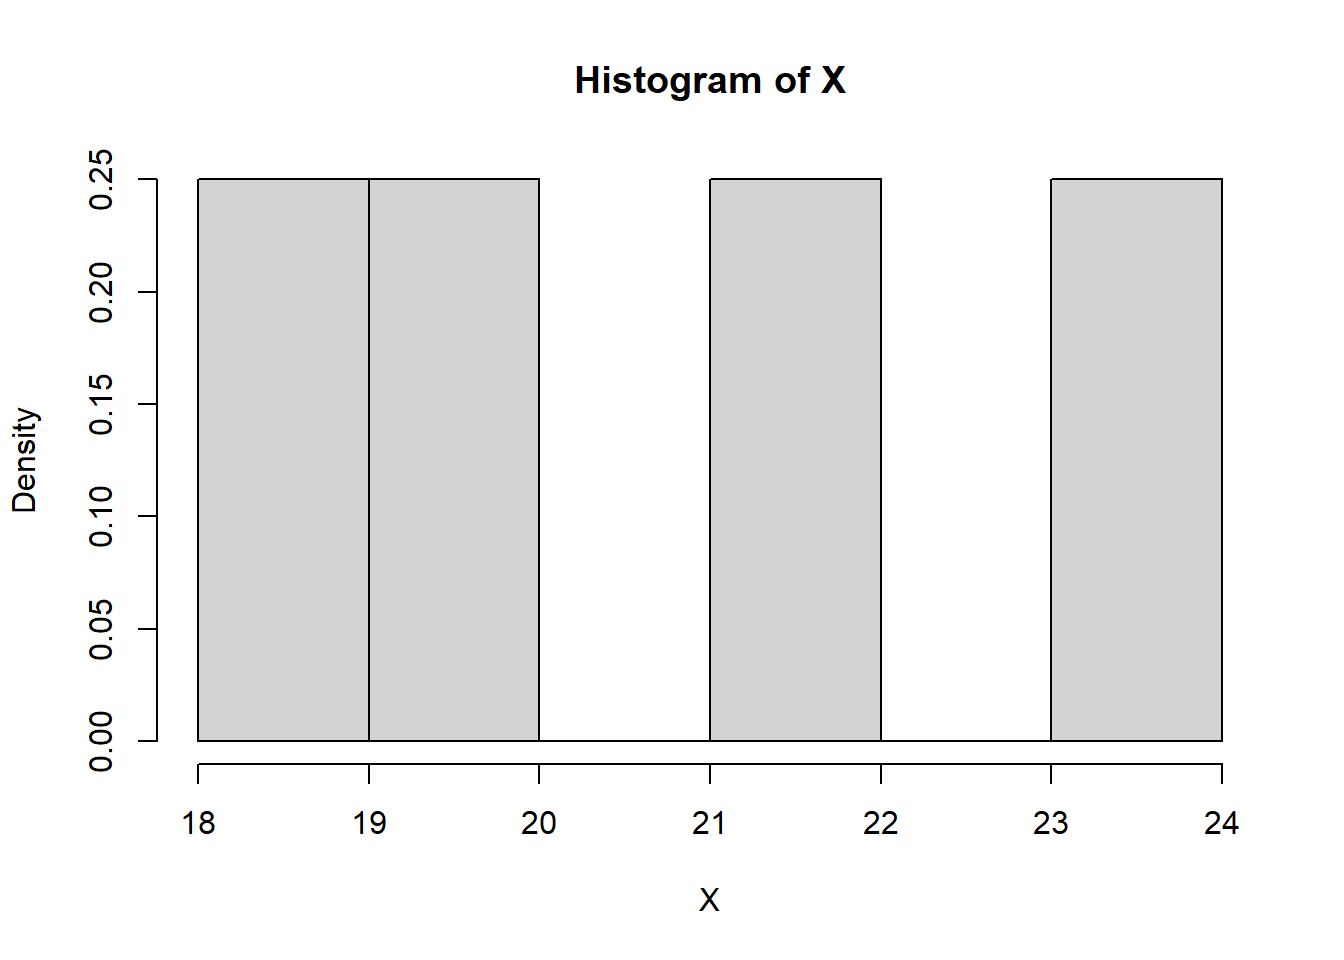
\includegraphics[width=1\linewidth,height=0.4\textheight]{bookdown_files/figure-latex/unnamed-chunk-14-1}

建立n=2的抽样分布,样本均值分布如下,均值为21,方差为1.58。

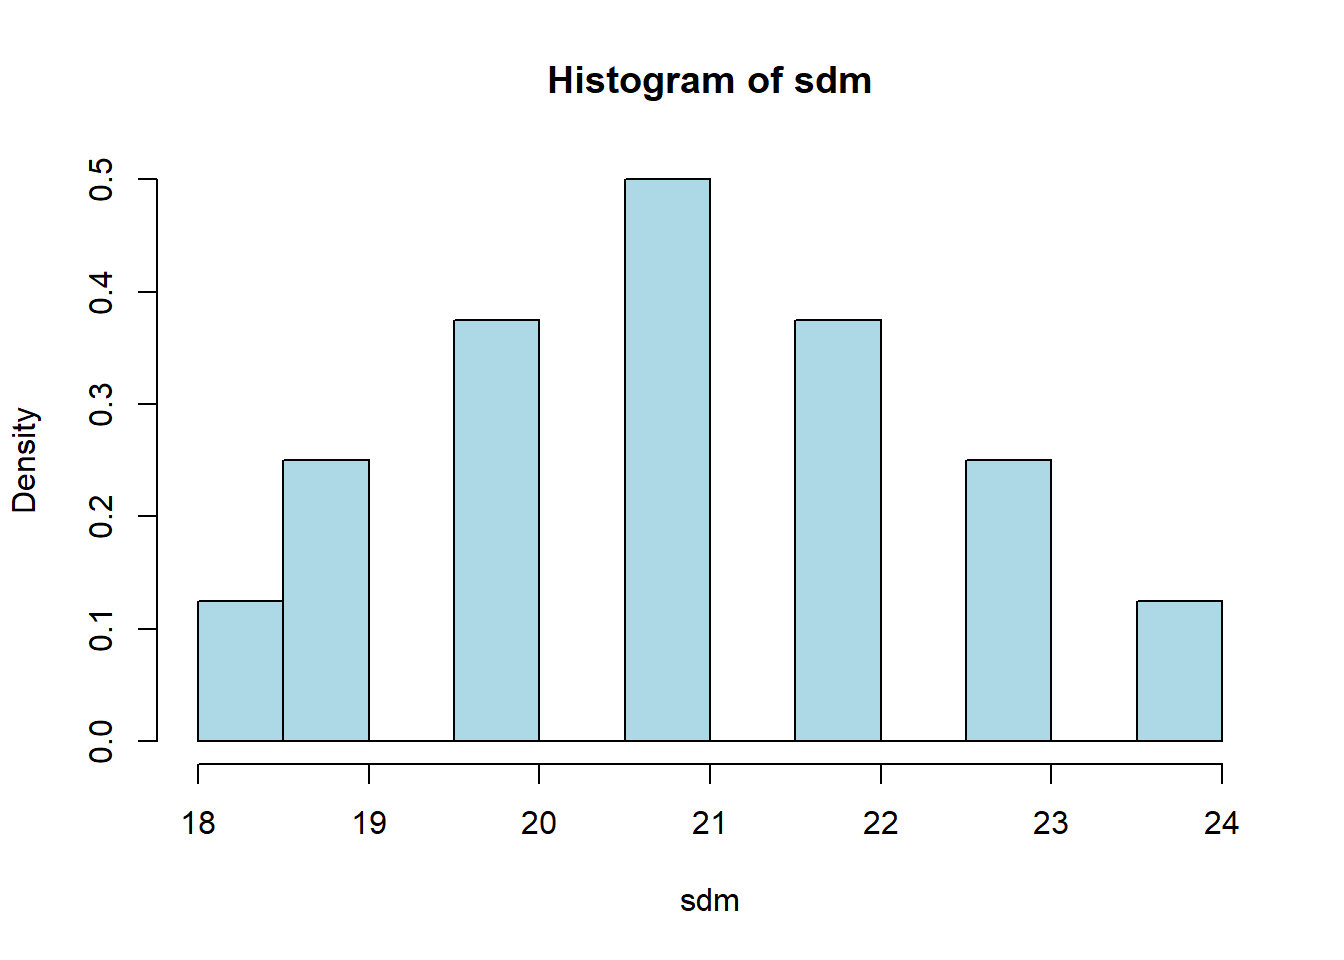
\includegraphics[width=1\linewidth,height=0.4\textheight]{bookdown_files/figure-latex/unnamed-chunk-15-1}

可以发现总体分布是均匀分布,而样本均值的抽样分布却呈现了近似正态分布,均值是相同的,但是方差却有差异。根据总体分布以及样本容量可以将抽样分布分为以下三类:

\begin{quote}
\begin{itemize}
\tightlist
\item
  精确抽样分布:当总体分布已知时,如果对任一自然数都能导出统计量分布的显示表达式,这样的抽样分布称为精确抽样分布(对小样本的统计推断特别有用,大多数是在正态总体下得到的, t分布、 F分布等)。
\item
  渐近抽样分布:样本量无限大时统计量的极限分布(大样本问题)。
\item
  近似抽样分布:注意获得近似分布的条件(用统计量的前二阶矩当作正态分布的前二阶矩获得
  正态近似,随机模拟法获得统计量的近似分布)。
\end{itemize}
\end{quote}

\hypertarget{ux4e00ux4e2aux603bux4f53ux6837ux672cux7edfux8ba1ux91cfux7684ux62bdux6837ux5206ux5e03}{%
\section{一个总体样本统计量的抽样分布}\label{ux4e00ux4e2aux603bux4f53ux6837ux672cux7edfux8ba1ux91cfux7684ux62bdux6837ux5206ux5e03}}

样本均值的抽样分布------在重复选取容量为 n 的样本时,由样本均值的所有可能取值形成的相对频数分布(一种理论概率分布,推断总体均值的理论基础)。

\begin{quote}
\begin{itemize}
\tightlist
\item
  正态总体均值抽样分布------精确分布(均值无偏)。
\item
  样本均值的中心极限定理------渐进分布。
\end{itemize}
\end{quote}

中心极限定理:
设从均值为\(\mu\), 方差为\(\sigma^2\)的一个任意总体中抽取容量为n的样本,当n充分大时,样本均值的抽样分布近似服从均值为\(\mu\)、 方差为\(\sigma^2/n\)的正态分布。

用一张图来说明这个定理(摘自参考书目1:贾俊平,《统计学》(第五版),中国人民大学出版社,2012.)。

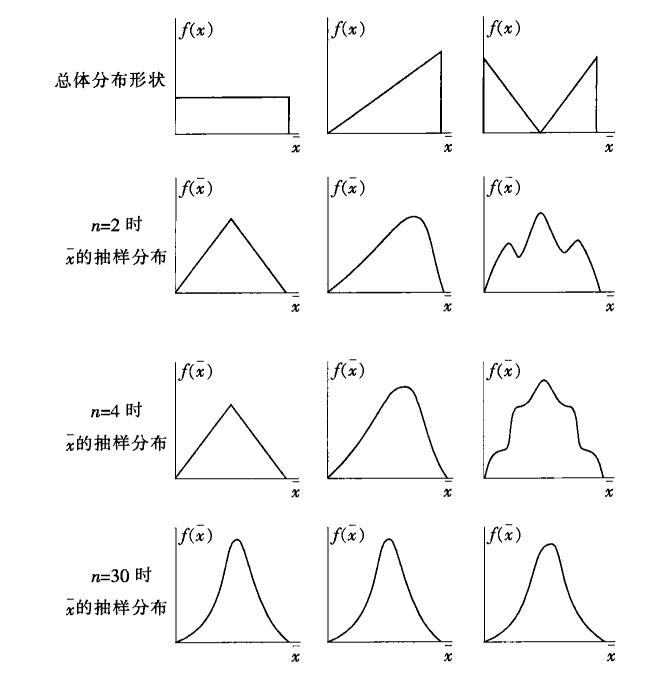
\includegraphics[width=1\linewidth,height=0.6\textheight]{fig/fig7}

当然也在这里诞生了一个统计学闻名于世的规定,样本容量n一般至少要求\textgreater30。因此样本均值的抽样分布中,样本均值的数学期望(也就是均值)和方差就有对应的公式了。样本均值的数学期望和方差如下。

数学期望:

\[E(\bar x) =\mu\]

方差:

\[\sigma_{\bar x}^2=\frac{\sigma^2}{n}\] (重复抽样),

\[\sigma_{\bar x}^2=\frac{\sigma^2}{n}\frac{N-n}{N-1}\](样本总体有限,且\(n\ge 5\%N\)不重复抽样)

总结来说,总体分布为正态分布的话,抽样分布也是正态分布,总体分布为非正态分布的话,大样本情况下也是近似正态分布,小样本则为非正态分布。除了均值之外,实际生活中比例也是一个很重要的参数。比例------总体(或样本)中具有某种属性的单位与全部单位总数之比(如不同性别的人与全部人数之比,合格品(或不合格品) 与全部产品总数之比)。总体比例可表示为\(p=\frac{N_0}{N},1-p=\frac{N_1}{N}\),样本比例可表示为\(p=\frac{n_0}{n},1-p=\frac{n_1}{n}\)。

样本比例的抽样分布------在重复选取容量为n的样本时,由样本比例的所有可能取值形成的相对频数分布。

\begin{quote}
\begin{itemize}
\tightlist
\item
  一种理论概率分布。
\item
  当样本容量很大时(满足np≥5, n(1-p)≥5),样本比例的抽样分布可用正态分布近似。
\item
  推断总体比例p的理论基础。
\end{itemize}
\end{quote}

类似于均值的抽样分布我们可以得到样本比例的数学期望和方差。

数学期望:

\[E(\bar p) =p\]

方差:

\[\sigma_{\bar x}^2=\frac{p(1-p)}{n}\] (重复抽样),
\[\sigma_{\bar x}^2=\frac{p(1-p)}{n}\frac{N-n}{N-1}\](不重复抽样)

接下来介绍一个重要的分布------卡方分布。若随机变量\(\xi_1,\xi_2,\cdots,\xi_n\)是n个相互独立的标准正态变量(独立同分布于标准正态分布),则这n个随机变量的平方和\(Y=\Sigma\xi_i^2\)构成的随机变量的分布称为自由度为n的\(\chi^2\)分布(chi-square distribution),记为\(\chi^2(n)\)分布。卡方分布的性质和特点如下:

\begin{quote}
\begin{itemize}
\tightlist
\item
  分布的变量值始终为正
\item
  分布的形状取决于其自由度n的大小, 通常为不对称的单峰右偏( 正偏) 分布, 但随着自由度的增大逐渐趋于对称, 当n\textgreater30时, 接近正态分布。
\item
  期望为: \(E(\chi^2)=n\),方差为: \(D(\chi^2)=2n\)(n为自由度)
\item
  可加性:若U和V为两个独立的\(\chi^2\)分布随机变量,\(U\sim \chi^2(n_1)\),\(V\sim \chi^2(n_2)\), 则U+V这一随机变量服从自由度为\(n_1+n_2\)的\(\chi^2\)分布
\end{itemize}
\end{quote}

卡方分布的性质可以根据这张图来看。

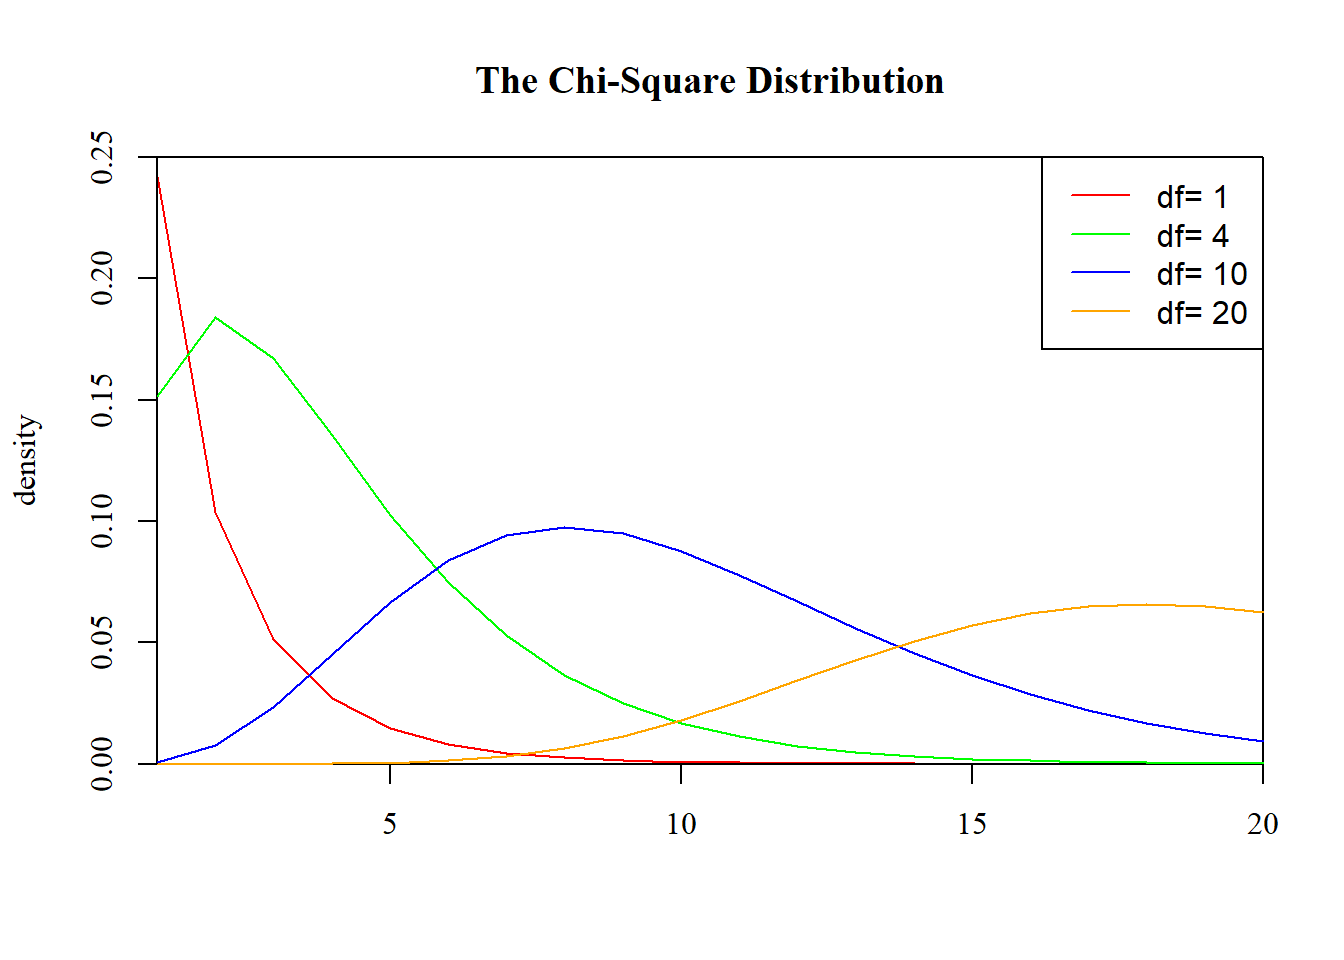
\includegraphics[width=1\linewidth,height=0.4\textheight]{bookdown_files/figure-latex/unnamed-chunk-17-1}

卡方分布一般用于样本方差的分布的计算。样本方差的分布------在重复选取容量为n的样本时, 由样本方差的所有可能取值形成的相对频数分布。对于来自正态总体的简单随机样本,则比值\(\frac{(n-1)s^2}{\sigma^2}\),该比值的抽样分布服从自由度为(n-1)的\(\chi^2\)分布,即\(\frac{(n-1)s^2}{\sigma^2}\sim \chi^2(n-1)\)。

接着再介绍一个耳熟能详的t分布。t 分布是类似正态分布的一种对称分布, 它通常要比正态分布平坦和分散。 t分布的性质和特点如下:

\begin{quote}
\begin{itemize}
\tightlist
\item
  自由度为1的t 分布为柯西分布,期望值不存在。
\item
  n\textgreater1时,期望值为0。
\item
  n\textgreater2时,方差存在,为n/(n-2)。
\item
  随着自由度的增大,分布也逐渐趋于标准正态分布。(t 分布的极限为标准正态分布,当n\textgreater30时, t 分布可用标准正态分布近似)
\end{itemize}
\end{quote}

t分布的性质可以根据这张图来看。

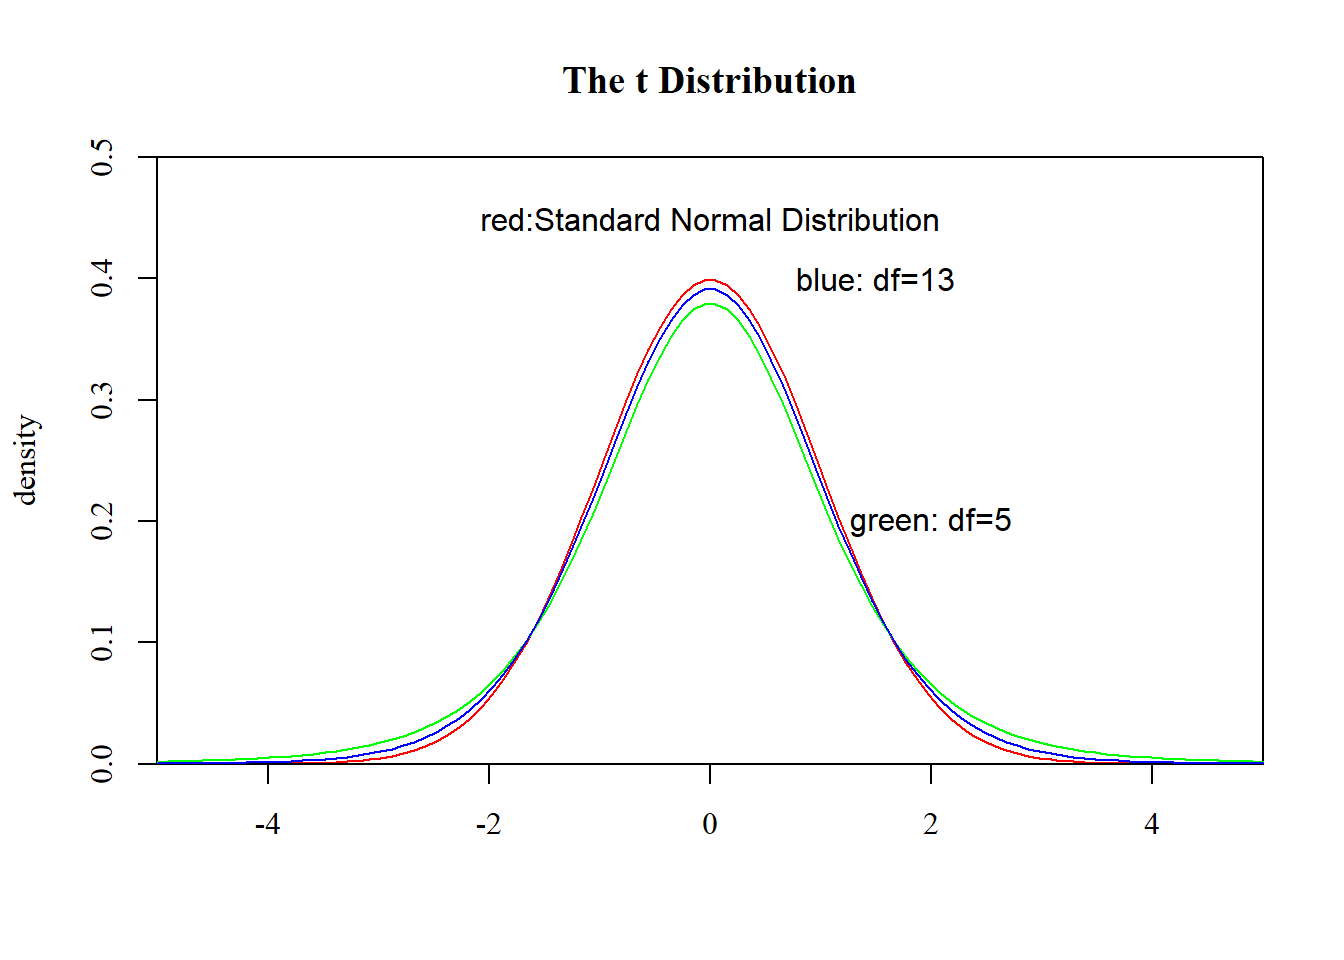
\includegraphics[width=1\linewidth,height=0.4\textheight]{bookdown_files/figure-latex/unnamed-chunk-18-1}

t分布的应用是在求样本均值与样本标准差之比上,样本均值与样本标准差之比的分布为:\(t=\frac{\bar x-\mu}{s/\sqrt{n}}\sim t(n-1)\),自由度为(n-1)的t分布。

\hypertarget{ux4e24ux4e2aux603bux4f53ux6837ux672cux7edfux8ba1ux91cfux7684ux62bdux6837ux5206ux5e03}{%
\section{两个总体样本统计量的抽样分布}\label{ux4e24ux4e2aux603bux4f53ux6837ux672cux7edfux8ba1ux91cfux7684ux62bdux6837ux5206ux5e03}}

其实从前面第4点内容可以看出,其实实际应用中,均值、比例、方差的估计是比较多的,因此这三个总体样本统计量的抽样分布特别提出来了。而第4点讨论的是一个总体的,两个总体的也可以类比,道理是一样的。两个样本均值之差的抽样分布:

\begin{quote}
\begin{itemize}
\tightlist
\item
  两个总体均为正态分布,即\(X_1\sim N(\mu_1,\sigma_1^2),X_2\sim N(\mu_2,\sigma_2^2)\)。
\item
  两个样本均值之差的抽样分布服从正态分布,其分布的数学期望为两个总体均值之差:\(E(\bar x_1-\bar x_2)=\mu_1-\mu_2\)
\item
  方差为各自的方差之和:\(\sigma_{\bar x_1-\bar x_2}^2=\frac{\sigma_1^2}{n_1}+\frac{\sigma_2^2}{n_2}\)
\end{itemize}
\end{quote}

两个样本比例之差的抽样分布:

\begin{quote}
\begin{itemize}
\tightlist
\item
  两个总体都服从二项分布。
\item
  分别从两个总体中抽取容量为\(n_1\)和\(n_2\)的独立样本,当两个样本都为大样本时,两个样本比例之差的抽样分布可用正态分布来近似。
\item
  分布的数学期望为:\(E(\bar p_1-\bar p_2)=p_1-p_2\)。
\item
  方差为各自方差之和:\(\sigma_{\bar p_1-\bar p_2}^2=\frac{p_1(1-p_1)}{n_1}+\frac{p_2(1-p_2)}{n_2}\)。
\end{itemize}
\end{quote}

最后的最后,我们来介绍本片的最后一个重要的分布------F分布。F分布:设若U为服从自由度为\(n_1\)的\(\chi^2\)分布,即\(U\sim \chi^2(n_1)\), V为服从自由度为\(n_2\)的\(\chi^2\)分布,即\(V\sim \chi^2(n_2)\),且U与V相互独立, \(F=\frac{U/n_1}{V/n_2}\),F服从自由度\(n_1\)和\(n_2\)的F分布, 记为\(F\sim F(n_1,n_2)\)。

不同自由度下的F分布

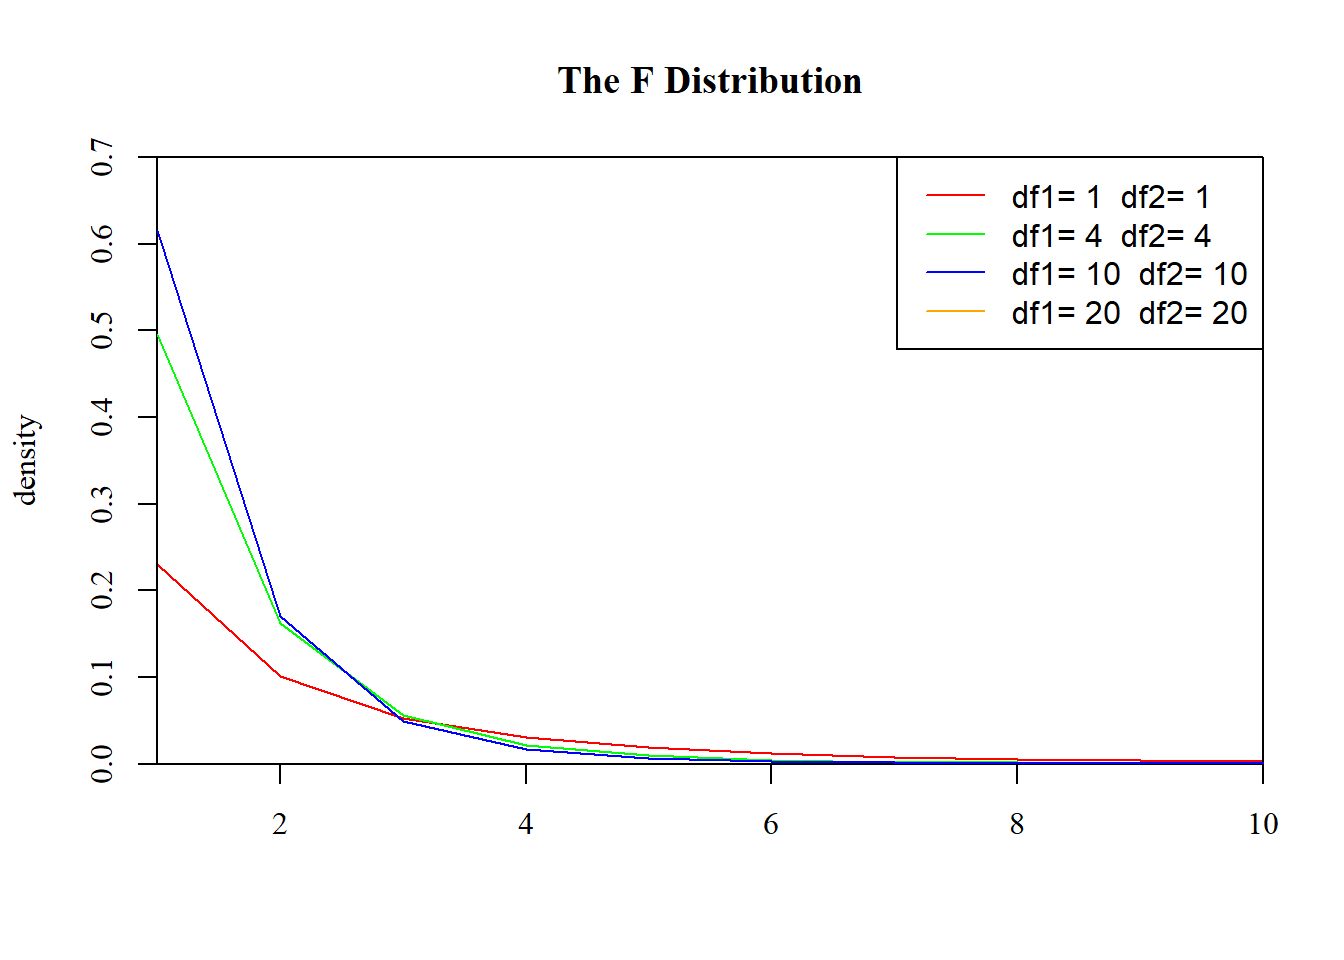
\includegraphics[width=1\linewidth,height=0.4\textheight]{bookdown_files/figure-latex/unnamed-chunk-19-1}

两个样本方差比的抽样分布:
\textgreater{} * 两个总体都为正态分布,即\(X_1\sim N(\mu_1,\sigma_1^2), X_2\sim N (\mu_2,\sigma_2^2)\)。
\textgreater{} * 从两个总体中分别抽取容量为\(n_1\)和\(n_2\)的独立样本。
\textgreater{} * 两个样本方差比的抽样分布,服从分子自由度\((n_1-1)\),分母自由度为\((n_2-1)\)的F分布, 即\(\frac{s_1^2/\sigma_1^2}{s_2^2/\sigma_2^2}\sim F(n_1-1,n_2-1)\)

\hypertarget{ux9644ux5f55}{%
\section{附录}\label{ux9644ux5f55}}

常用统计量公式

样本均值:

\[\bar X=\frac{1}{n} \sum_{i=1}^n{X_i}\]

样本方差:

\[S^2=\frac{1}{n-1} \sum_{i=1}^n(X_i-\bar X)^2\]

样本标准差:

\[S=\sqrt{\frac{1}{n-1} \sum_{i=1}^n(X_i-\bar X)^2}\]

样本k阶原点矩:

\[A_k=\frac{1}{n} \sum_{i=1}^nX_i^k(k=1,2,\cdots)\]

样本k阶中心矩:

\[B_k=\frac{1}{n} \sum_{i=1}^n(X_i-\bar X)^k(k=1,2,\cdots)\]

各统计量的观察值:

\[\bar x=\frac{1}{n} \sum_{i=1}^n{x_i}\]

\[s^2=\frac{1}{n-1} \sum_{i=1}^n(x_i-\bar x)^2\]

\[a_k=\frac{1}{n} \sum_{i=1}^nx_i^k(k=1,2,\cdots)\]

\[b_k=\frac{1}{n} \sum_{i=1}^n(x_i-\bar x)^k(k=1,2,\cdots)\]

\hypertarget{estimation}{%
\chapter{Estimation}\label{estimation}}

本篇是第五章,内容是参数估计。

\hypertarget{ux53c2ux6570ux4f30ux8ba1ux7684ux4e00ux822cux95eeux9898}{%
\section{参数估计的一般问题}\label{ux53c2ux6570ux4f30ux8ba1ux7684ux4e00ux822cux95eeux9898}}

正如前面介绍的,统计学的两大分支,分别是描述统计和推断统计。所以今天来谈谈推断统计的第一大问题------参数估计。当然一般叫统计推断的会更多些,二者是一样的。统计推断(Statistical Inference)------主要包括参数估计和假设检验,实质就是通过样本的均值、标准差、方差等去估计总体的均值、标准差、方差或者判断总体的分布形式和分布参数。

\begin{quote}
\begin{itemize}
\tightlist
\item
  参数估计:根据从总体中抽得的样本所提供的信息,对总体分布中包含的未知参数作出数值上的估计。
  点估计:用样本的某一函数值来估计总体分布中的未知参数;
  区间估计:按照一定的可靠度估计出参数的一个范围,即确定一个区间,使这一个区间内包含参数真值的概率达到预先所要求的程度。
\item
  假设检验:需要对总体的分布形式或分布参数事先作出某种假设,然后根据样本观测值,运用统计分析的方法来检验这一假设是否正确。
\end{itemize}
\end{quote}

上一篇提到的,获取样本之后,我们需要去猜总体,参数估计就是猜总体的参数(分布中所含的未知参数;分布特征:均值、方差等;事件的概率等)或者参数空间(参数的可能取值范围)。假设检验是下一章内容,这里就不细述了。首先明确两个概念:估计量(estimator)与估计值(estimated value)。

\begin{quote}
\begin{itemize}
\tightlist
\item
  估计量: 用于估计总体参数的随机变量,一般为样本统计量(如样本均值、 样本比例、 样本方差等; 例如:样本均值就是总体均值\(\mu\)的一个估计量)。
\item
  估计值: 估计参数时计算出来的统计量的具体值,如果样本均值=80, 则80就是总体均值的估计值。
\end{itemize}
\end{quote}

既然是估计量,就必须有评价估计量的标准。一般包括以下几点:

\begin{quote}
\begin{itemize}
\tightlist
\item
  无偏性:估计量的数学期望等于被估计的总体参数,样本的随机性导致估计偏差, 偏差平均值为0, 无系统误差(所以在这里又提出了渐进无偏估计:估计随着样本量的增加而逐渐趋近于真值。渐进无偏估计指系统偏差会随着样本量的增加而逐渐减小,趋于0,在大样本时可近似当无偏估计使用)。
\item
  有效性: 对同一总体参数的两个无偏点估计量, 有更小标准差的估计量更有效。
\item
  一致性: 随着样本容量的增大, 估计量的值越来越接近被估计的总体参数。
\end{itemize}
\end{quote}

由于无偏性是最普遍的标准。这里再介绍部分无偏性的几个要点:

\begin{quote}
\begin{itemize}
\tightlist
\item
  样本均值是总体期望的无偏估计。
\item
  诸观测值对样本均值的偏差可正可负,其和恒为0(n个偏差中只有n-1个是独立的)。
\item
  自由度:独立偏差个数。
\item
  偏差平方和(样本量相等情况下,偏差平方和的大小反映样本散布的大小, 样本量大,偏差平方和大趋近于平均偏差平方和,偏差平方和的期望小于方差,有偏估计,渐进无偏估计。
\end{itemize}
\end{quote}

点估计(point estimate)

\begin{quote}
\begin{itemize}
\tightlist
\item
  用样本估计量的某个取值直接作为总体参数的估计值(例如:用样本均值直接作为总体均值的估计;用两个样本均值之差直接作为总体均值之差的估计)。
\item
  无法给出估计值接近总体参数程度的信息(虽然在重复抽样条件下,点估计的均值可望接近总体真值,但由于样本是随机的,抽出一个具体的样本得到的估计值等同于总体真值的可能性很小,特别是在连续分布时,该概率几乎为0,一个点估计量的可靠性是由它的抽样标准误差来衡量的,这表明一个具体的点估计值无法给出估计的可靠性的度量)。
\end{itemize}
\end{quote}

\hypertarget{ux533aux95f4ux4f30ux8ba1-confidence-intervals}{%
\section{区间估计 Confidence Intervals}\label{ux533aux95f4ux4f30ux8ba1-confidence-intervals}}

正如前面提到的点估计可靠性较低,因此在点估计的基础上又提出了区间估计(interval estimate),它能解决的问题包括:

\begin{quote}
\begin{itemize}
\tightlist
\item
  为解决参数估计的精确度和可靠性问题, 在点估计的基础上给出总体参数估计的一个区间范围(该区间一般由样本统计量加减抽样误差而得到),使这一个区间内包含参数真值的概率大到预先所要求的程度。
\item
  它不具体指出总体参数等于什么,但能指出总体的未知参数落入某一区间的概率有多大。
\end{itemize}
\end{quote}

二者的区别在于:点估计是一个数,区间估计给出一个区间,提供更多关于变异性的信息。通俗的解释,你女朋友买了件衣服,让你猜价格,你猜中准确价格很难,但是你猜一个范围还是准确度比较高的。

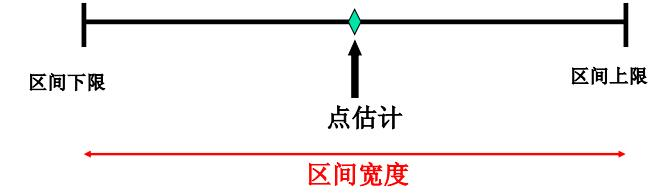
\includegraphics[width=1\linewidth,height=0.3\textheight]{fig/fig8}

所以区间估计(interval estimate)的概念是------根据样本统计量的抽样分布能够对样本统计量与总体参数的接近程度给出一个概率度量。由概率度量则引出了置信区间(Confidence Intervals)的概念。设\(x_1,x_2,\cdots,x_n\)是来自\(f(x,\theta)\)的样本,对于给定的\(\alpha,0<\alpha<1\),如能找到两个统计量\(\theta_1(x_1,x_2,\cdots,x_n)\)和\(\theta_2(x_1,x_2,\cdots,x_n)\)使得\(P\left\{(\theta_1(x_1,x_2,\cdots,x_n)<\theta<\theta_2(x_1,x_2,\cdots,x_n)\right\}\ge1-\alpha\), 称\((\theta_1(x_1,x_2,\cdots,x_n),\theta_2(x_1,x_2,\cdots,x_n))\)是\(\theta\)的置信度为\(1-\alpha\)的置信区间(Confidence interval);\(\theta_1,\theta_2\)为置信上限与置信下限,\(1-\alpha\)为置信度,\(\alpha\)为显著性水平(Significance level)。

置信区间实质上是由样本统计量所构造的总体参数的估计区间。在某种程度上确信这个区间包含真正的总体参数(用一个具体的样本所构造的区间是一个特定的区间,我们无法知道这个样本所产生的区间是否包含总体参数的真值,我们只能是希望这个区间是大量包含总体参数真值的区间中的一个,但它也可能是少数几个不包含参数真值的区间中的一个)。置信区间表明了区间估计的精确性, 区间越小越精确,区间越大越不精确。置信水平------将构造置信区间的步骤重复很多次,置信区间包含总体参数真值的次数所占的比例称为置信水平(置信度)。置信水平表明了区间估计的可靠性,表示为\((1-\alpha)\),\(\alpha\)是总体参数未在区间内的比例, 区间估计不可靠的概率为\(\alpha\), 如\(\alpha\)=0.05, 表明结论犯错误的概率为0.05),常用的置信水平值有99\%, 95\%, 90\%。那么什么样的置信区间是好的置信区间呢?也就是区间估计的评价标准是什么呢?一般包括如下两点:

\begin{quote}
\begin{itemize}
\tightlist
\item
  置信度(置信系数)越大越好------概率越大越放心,但不能一味求大。
\item
  随机区间平均长度越短越好------估计精度越高。
\end{itemize}
\end{quote}

但是在某些实际问题中,我们可能更关心置信上限或置信下限(合金钢强度,越大越好(望大特性),平均强度下限是个重要指标,药物毒性,越小越好(望小特性),平均毒性上限是个重要指标)。这就是单侧置信限问题。谈完了这么多理论,接下来进入实践,如何做一个总体参数的区间估计?
按照前一章,我们还是讨论三个重要的总体参数:均值、比例、方差。也是先谈一个总体参数的区间估计。首先规定好符号对应统计量和参数。

总体均值------\(\mu\),总体比例------p,总体方差------\(\sigma^2\);样本均值------\(\bar x\),样本比例------\(\bar p\),样本方差------\(s^2\)。

\begin{itemize}
\tightlist
\item
  一个总体均值的置信区间估计方法总结起来就是:
\end{itemize}

\begin{quote}
\begin{itemize}
\tightlist
\item
  正态分布,且总体方差\(\sigma\)已知,用Z值;
\item
  正态分布,且总体方差\(\sigma\)未知,用t值;
\item
  非正态分布但是大样本,无论总体方差\(\sigma\)是否已知,用Z值。
\end{itemize}
\end{quote}

第一种情况:正态分布统计量z------\(z=\frac{\bar x-\mu}{\sigma/\sqrt{n}}\sim N(0,1)\),总体均值\(\mu\)在\(1-\alpha\)置信水平下的置信区间为\(\bar x\pm z_{\alpha/2}\frac{\sigma}{\sqrt{n}}\),置信下限为\(\bar x- z_{\alpha/2}\frac{\sigma}{\sqrt{n}}\),置信上限为\(\bar x+ z_{\alpha/2}\frac{\sigma}{\sqrt{n}}\)。

第二种情况:t分布统计量------\(t=\frac{\bar x-\mu}{s/\sqrt{n}}\sim t(n-1)\),总体均值\(\mu\)在\(1-\alpha\)置信水平下的置信区间为\(\bar x\pm t_{\alpha/2}\frac{s}{\sqrt{n}}\),置信下限为\(\bar x- t_{\alpha/2}\frac{s}{\sqrt{n}}\),置信上限为\(\bar x+ t_{\alpha/2}\frac{s}{\sqrt{n}}\)。

第三种情况:正态分布统计量z------\(z=\frac{\bar x-\mu}{\sigma/\sqrt{n}}\sim N(0,1)\),总体均值\(\mu\)在\(1-\alpha\)置信水平下的置信区间为\(\bar x\pm z_{\alpha/2}\frac{\sigma}{\sqrt{n}}\)(\(\sigma\)未知的话,把\(\sigma\)换成s即可)。

\begin{itemize}
\tightlist
\item
  一个总体比例的置信区间估计方法
\end{itemize}

假定条件\(np\geq5\), \(n(1-p)\geq5\), \(n\geq30\)。正态分布统计量z------\(z=\frac{\bar p-p}{\sqrt{\frac{p(1-p)}{n}}}\sim N(0,1)\),总体比例的置信区间为

\[\bar p\pm z_{\alpha/2}\sqrt{\frac{p(1-p)}{n}}\]

或

\[\bar p\pm z_{\alpha/2}\sqrt{\frac{\bar p(1-\bar p)}{n}}\]。

\begin{itemize}
\tightlist
\item
  一个正态总体方差的置信区间估计方法
\end{itemize}

总体方差\(\sigma^2\)的点估计量为\(s^2\),则\(\frac{(n-1)s^2}{\sigma^2}\sim \chi^2(n-1)\),总体方差在\(1-\alpha\)置信水平下的置信区间为:

\[\frac{(n-1)s^2}{\chi^2_{\alpha/2}(n-1)}\le \sigma^2 \le \frac{(n-1)s^2}{\chi^2_{1-\alpha/2}(n-1)}\]

接下来谈谈两个总体参数的置信区间的估计方法。估计的一般包括均值差、比例差、方差比,主要包括两种抽样方法------独立样本和配对样本。

\begin{itemize}
\tightlist
\item
  两个正态总体均值之差的置信区间(独立样本):
\end{itemize}

\(\sigma_1^2\),\(\sigma_2^2\)已知,使用正态分布统计量z:\(z=\frac{(\bar x_1-\bar x_2)-(\mu_1-\mu_2)}{\sqrt{\frac{\sigma_1^2}{n_1}+\frac{\sigma_2^2}{n_2}}}\sim N(0,1)\),两个总体均值之差\(\mu_1-\mu_2\)在\(1-\alpha\)置信水平下的置信区间为:

\[(\bar x_1-\bar x_2)\pm z_{\alpha/2}\sqrt{\frac{\sigma_1^2}{n_1}+\frac{\sigma_2^2}{n_2}}\]。

\(\sigma_1^2=\sigma_2^2\)未知,总体方差的合并估计量:\(s_p^2=\frac{(n_1-1)s_1^2+(n_2-1)s_2^2}{n_1+n_2-2}\),估计量\(\bar x_1-\bar x_2\)的抽样标准差:\(\sqrt{\frac{sp_1^2}{n_1}+\frac{sp_2^2}{n_2}}\),两个样本均值之差的标准化:\(t=\frac{(\bar x_1-\bar x_2)-(\mu_1-\mu_2)}{s_p\sqrt{\frac{1}{n_1}+\frac{1}{n_2}}}\sim t(n_1+n_2-2)\),两个总体均值之差\(\mu_1-\mu_2\)在\(1-\alpha\)置信水平下的置信区间为:

\[(\bar x_1-\bar x_2)\pm t_{\alpha/2}(n_1+n_2-2)\sqrt{s_p^2(\frac{1}{n_1}+\frac{1}{n_2})}\]。

\(\sigma_1^2\neq\sigma_2^2\)未知,\(n_1=n_2: (\bar x_1-\bar x_2)\pm t_{\alpha/2}(n_1+n_2-2)\sqrt{(\frac{s_1^2}{n_1}+\frac{s_2^2}{n_2})}\)。

\(\sigma_1^2\neq\sigma_2^2\)未知,\(n_1\neq n_2\):\((\bar x_1-\bar x_2)\pm t_{\alpha/2}(v)\sqrt{(\frac{s_1^2}{n_1}+\frac{s_2^2}{n_2})}\), v为自由度,\(v=\frac{(\frac{s_1^2}{n_1}+\frac{s_2^2}{n_2})^2}{\frac{(s_1^2/n_1)^2}{n_1-1}+\frac{(s_2^2/n_2)^2}{n_2-1}}\)。

\begin{itemize}
\tightlist
\item
  两个总体均值之差的区间估计(独立大样本)两个总体均值之差的估计
\end{itemize}

\(\sigma_1^2\),\(\sigma_2^2\)已知时,两个总体均值之差\(\mu_1-\mu_2\)在\(1-\alpha\)置信水平下的置信区间为:

\[(\bar x_1-\bar x_2)\pm z_{\alpha/2}\sqrt{(\frac{\sigma_1^2}{n_1}+\frac{\sigma_2^2}{n_2})}\]。

\(\sigma_1^2\),\(\sigma_2^2\)未知时,两个总体均值之差\(\mu_1-\mu_2\)在\(1-\alpha\)置信水平下的置信区间为:

\[(\bar x_1-\bar x_2)\pm z_{\alpha/2}\sqrt{(\frac{s_1^2}{n_1}+\frac{s_2^2}{n_2})}\]。

两个总体均值之差的区间估计(匹配样本),匹配大样本的假定条件------两个匹配的大样本(\(n_1\ge30\)和\(n_2\ge30\));

两个总体均值之差\(\mu_d=\mu_1-\mu_2\)在\(1-\alpha\)置信水平下的置信区间为:

\[\bar d\pm z_{\alpha/2}\frac{\sigma_d}{\sqrt{n}}\]

或

\[\bar d\pm z_{\alpha/2}\frac{s_d}{\sqrt{n}}\]。

\(\bar d\)为对应差值的均值,\(\sigma_d\)为对应差值的标准差。

匹配小样本的假定条件------两个匹配的小样本(\(n_1<30\)和\(n_2<30\)),两个总体各观察值的配对差服从正态分布。两个总体均值之差\(\mu_d=\mu_1-\mu_2\)在\(1-\alpha\)置信水平下的置信区间为:

\[\bar d\pm t_{\alpha/2}(n-1)\frac{s_d}{n}\]

两个总体比例之差区间的估计,假定条件------两个总体服从二项分布,可以用正态分布来近似,两个样本是独立的。

两个总体比例之差\(p_1-p_2\)在\(1-\alpha\)置信水平下的置信区间为:

\[\bar p_1-\bar p_2\pm z_{\alpha/2}\sqrt{\frac{\bar q_1(1-\bar q_1)}{n_1}+\frac{\bar q_2(1-\bar q_2)}{n_2}}\]。

两个正态总体方差比的置信区间,实际应用如两种不同方法生产的产品性能的稳定性或两种不同测量工具的精度,需要我们去比较两个总体方差。

两个正态总体方差比的估计,比较两个总体的方差比,用两个样本的方差比来判断(如果\(s_1^2/s_2^2\)接近于1,说明两个总体方差很接近;如果\(s_1^2/s_2^2\)远离1,说明两个总体方差存在差异)。

总体方差比在\(1-\alpha\)置信水平下的置信区间为:

\[\frac{s_1^2/s_2^2}{F_{\alpha/2}}<\frac{\sigma_1^2}{\sigma_2^2}<\frac{s_1^2/s_2^2}{F_{1-\alpha/2}},F\sim F(n_1-1,n_2-1)\]

(F分布性质:\(F_{1-\alpha/2}(n_1,n_2)=\frac{1}{F_{\alpha/2}(n_2,n_1)}\))。

总的来说,参数估计的东西很多,根据具体研究情况,我们可以根据自己需求选择不同的参数估计。当然据笔者所知,R语言在参数估计上,现成函数(指默认的基础包)比较少,一般需要自编函数或者有额外的包。这里先给出一个样例函数(14章中会涉及到一部分,这里不详述)。

\begin{Shaded}
\begin{Highlighting}[]
\NormalTok{conf.int <-}\StringTok{ }\ControlFlowTok{function}\NormalTok{(x,sigma,alpha) \{}
\NormalTok{  mean =}\StringTok{ }\KeywordTok{mean}\NormalTok{(x)}
\NormalTok{  n =}\StringTok{ }\KeywordTok{length}\NormalTok{(x)}
\NormalTok{  z =}\StringTok{ }\KeywordTok{qnorm}\NormalTok{(}\DecValTok{1}\OperatorTok{-}\NormalTok{alpha}\OperatorTok{/}\DecValTok{2}\NormalTok{, }\DataTypeTok{mean =} \DecValTok{0}\NormalTok{, }\DataTypeTok{sd =} \DecValTok{1}\NormalTok{, }\DataTypeTok{lower.tail =}\NormalTok{ T)}
  \KeywordTok{c}\NormalTok{(mean}\OperatorTok{-}\NormalTok{sigma}\OperatorTok{*}\NormalTok{z}\OperatorTok{/}\KeywordTok{sqrt}\NormalTok{(n), mean}\OperatorTok{+}\NormalTok{sigma}\OperatorTok{*}\NormalTok{z}\OperatorTok{/}\KeywordTok{sqrt}\NormalTok{(n))}
\NormalTok{  \}}
\end{Highlighting}
\end{Shaded}

\hypertarget{ux6837ux672cux5bb9ux91cfux7684ux786eux5b9a}{%
\section{样本容量的确定}\label{ux6837ux672cux5bb9ux91cfux7684ux786eux5b9a}}

前一章我们提到统计学闻名于世的规定,样本容量一般必须>30。但是这种规定,并不是万能的。所以样本容量的确定就成了一个问题。n过大费用高、时间长、人力多;n过小误差增大。事实上n的确定依赖于多大置信度(可靠性),什么样的精度(多宽的区间)。所以样本容量的确定需要根据置信区间的性质来决定。置信区间的性质------以正态总体小样本容量为例。首先置信区间的宽度:\(w=2z\frac{\sigma}{\sqrt{n}}\),因此很容易发现影响区间宽度的因素包括了:

\begin{quote}
\begin{itemize}
\tightlist
\item
  样本容量:大样本容量------小区间。
\item
  总体数据的离散程度:小方差------小区间。
\item
  置信水平:高置信度------大t值------大区间。
\end{itemize}
\end{quote}

边际误差(margin error)------置信区间上下限与点估计之间的距离。

\[ E=z\frac{\sigma}{\sqrt{n}} \]

给定边际误差E和置信水平\(1-\alpha\),可以找到所需要的样本容量。

估计总体均值时样本容量的确定(\(\sigma^2\)已知):\(n=\frac{(z_{\alpha/2})^2\sigma^2}{E^2}\),其中\(E=z_{\alpha/2}\frac{\sigma}{\sqrt{n}}\)。

样本容量n与总体方差\(\sigma^2\)、边际误差E、置信水平\(1-\alpha\)之间的关系为:

\begin{quote}
\begin{itemize}
\tightlist
\item
  随总体方差增大而增大。
\item
  随边际误差减小而增大。
\item
  随\(1-\alpha\)增大而增大,随\(\alpha\)减小而增大。
\end{itemize}
\end{quote}

\(\sigma\)未知,如有近期样本可用,用其样本标准差代替\(\sigma\),用t分布分位数代替标准正态分布分位数,自由度为近期样本容量-1。否则,可以用一个至少比\(\sigma\)大的数来替代\(\sigma\),抽一个样本,用s代替\(\sigma\)------Stein 两步法。

估计总体比例时样本容量的确定:根据比例区间估计公式可得样本容量n为\(n=\frac{(z_{\alpha/2})^2\cdot p(1-p)}{E^2}\),其中:\(E=z_{\alpha/2}\sqrt{\frac{p(1-p)}{n}}\),E的取值一般小于0.1,p 未知时, 可用之前样本比率估计,或保守的取最大值0.5。

估计两个总体均值之差时样本容量的确定:设\(n_1\)和\(n_2\)为来自两个总体的样本,并假定\(n_1=n_2\)。根据均值之差的区间估计公式可得两个样本的容量n为:

\[n_1=n_2=n=\frac{(z_{\alpha/2})^2\cdot (\sigma_1^2+\sigma_2^2)}{E^2}\]

其中\(E=z_{\alpha/2}\sqrt{\frac{(\sigma_1^2+\sigma_2^2)}{n}}\)。

估计两个总体比例之差时样本容量的确定:设\(n_1\)和\(n_2\)为来自两个总体的样本,并假定\(n_1=n_2\)。根据比例之差的区间估计公式可得两个样本的容量n为:

\[n_1=n_2=n=\frac{(z_{\alpha/2})^2\cdot [p_1(1-p_1)+p_2(1-p_2)]}{E^2}\]

其中\(E=z_{\alpha/2}\sqrt{\frac{(p_1(1-p_1)+p_2(1-p_2))}{n}}\)。

总的来说,样本容量的确定也是根据具体需要以及显著性水平计算得到的。

\hypertarget{hypothesis}{%
\chapter{Hypothesis Test}\label{hypothesis}}

本篇是第6章,内容是假设检验。

\hypertarget{ux57faux672cux601dux60f3}{%
\section{基本思想}\label{ux57faux672cux601dux60f3}}

我们还是从问题开始讨论。这回提个接地气的问题------雄安新区批复前后对该地区房价是否有差异?嗯,假设检验其实就是为了解决这类问题。假设检验的基本思想------我们有样本,但是无法获得总体,需要对总体的分布形式或分布参数事先作出某种假设,然后根据样本观测值,运用统计分析的方法来检验这一假设是否正确。分解开来,假设检验=假设+检验(或者假设检验)。假设(hypothesis)------对总体的参数的具体数值(或分布形式)所作的陈述(总体参数包括总体均值、比例、 方差等,分析之前必需陈述)。假设检验(hypothesis test)---先对总体的参数( 或分布形式)提出某种假设,然后利用样本信息判断假设是否成立的过程(有参数检验和非参数检验;逻辑上运用反证法, 统计上依据小概率原理)。如图。

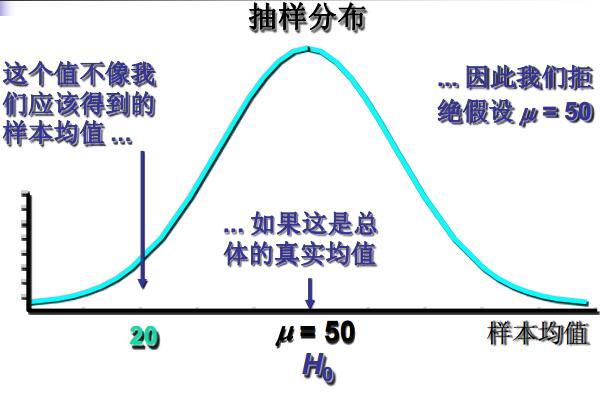
\includegraphics[width=1\linewidth,height=0.35\textheight]{fig/fig9}

假设检验的思想还可以去搜索Fisher 显著性检验的思想(女士品茶试验)的故事深深体会,这里就不详述了。有兴趣的同学可以点击下文的科学网链接查看。

\begin{quote}
\begin{itemize}
\tightlist
\item
  \url{http://blog.sciencenet.cn/blog-624263-795715.html}
\end{itemize}
\end{quote}

\hypertarget{ux539fux5047ux8bbeux548cux5907ux62e9ux5047ux8bbe}{%
\section{原假设和备择假设}\label{ux539fux5047ux8bbeux548cux5907ux62e9ux5047ux8bbe}}

从前面的介绍我们知道,假设检验的第一步是建立假设。那么假设分为两种(原假设和备择假设)。那么这二者具体又是什么呢?

\begin{quote}
\begin{itemize}
\tightlist
\item
  原假设(null hypothesis)------原假设又称`` 0假设'',总是有符号=, \(\geq\)或\(\leq\),表示为 \(H_0\)。是研究者想收集证据予以反对的假设(生产实践中常对应正常情形,如均值与设计一致);一般来说,原假设是一旦拒绝便要采取行动的假设。因此, 原假设总是``受到保护的假设'' ,没有充分的证据是不能拒绝原假设的。例如,对一家信誉很好的工厂的产品进行检验,原假设一般是`` 产品合格''。
\item
  备择假设(alternative hypothesis)------研究者想收集证据予以支持的假设, 一旦发生就要采取行动, 是与原假设对立的假设,也称``研究假设'',总是有符号\(\neq\), \textgreater{} 或 \textless,表示为 \(H_1\)。
\end{itemize}
\end{quote}

总结起来就是,原假设是统计学史上最悲催角色------它从一开始诞生,就是为了被科学家们发好人卡拒绝而存在的一个假设。备择假设才是科学家们追求的白富美。

搞明白了这两个假设,下一步我们做假设检验的时候,就要先提出假设了,这里给了一些提出假设的要点:
\textgreater{} * 原假设和备择假设是一个完备事件组, 而且相互对立(在一项假设检验中, 原假设和备择假设必有一个成立, 而且只有一个成立)。
\textgreater{} * 先确定备择假设, 再确定原假设。
\textgreater{} * 等号`` ='' 总是放在原假设上。
\textgreater{} * 因研究目的不同, 对同一问题可能提出不同的假设( 也可能得出不同的结论)。

同时在实际应用中,我们有不同的需求,因此又有双侧检验和单侧检验的区分。
\textgreater{} * 双侧检验------备择假设没有特定的方向性,并含有符号``=''的假设检验,称为双侧检验或双尾检验(two-tailed test)
\textgreater{} * 单侧检验------备择假设具有特定的方向性,并含有符号``\textgreater{}''或``\textless{}''的假设检验,称为单侧检验或单尾检验(one-tailed test)。其中备择假设的方向为``\textless{}'',称为左侧检验,备择假设的方向为``\textgreater{}'',称为右侧检验。

原假设与备择假设形式:
\textgreater{} * 双边检验:\(H_0: \mu=2,H_1: \mu\neq2\)。
\textgreater{} * 单边检验:左侧检验------\(H_0: \mu\ge2,H_1: \mu<2\),右侧检验------\(H_0: \mu\le2,H_1: \mu>2\)。

所见即所得,用一张图来表示假设检验过程。

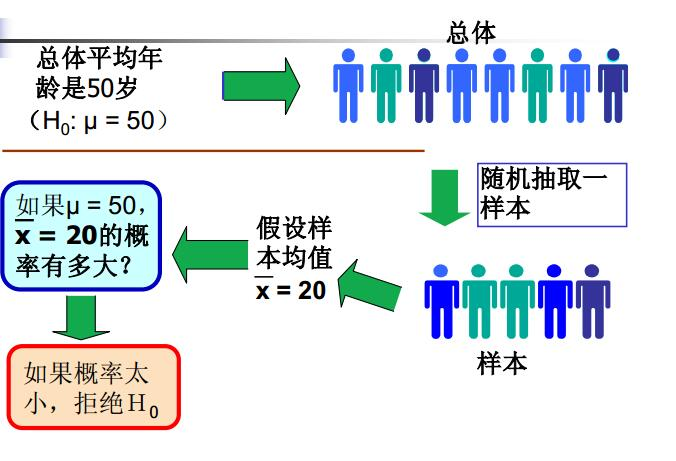
\includegraphics[width=1\linewidth,height=0.35\textheight]{fig/fig10}

所以拒绝原假设的理由是假设检验中的小概率原理。那么什么是小概率?

\begin{quote}
\begin{itemize}
\tightlist
\item
  在一次试验中, 一个几乎不可能发生的事件发生的概率。
\item
  在一次试验中小概率事件一旦发生, 我们就有理由拒绝原假设。
\item
  小概率由研究者事先确定。
\end{itemize}
\end{quote}

所以拒绝\(H_0\)的理由就是

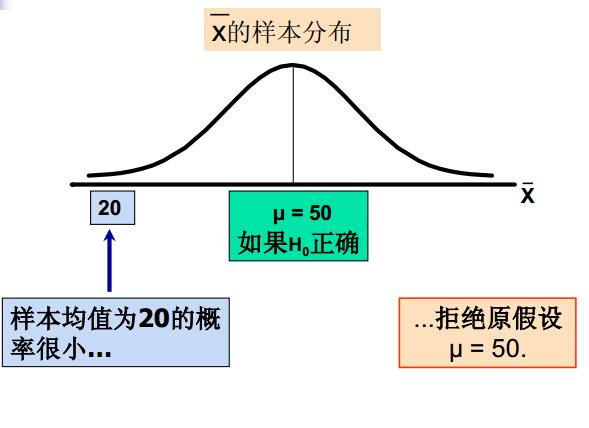
\includegraphics[width=1\linewidth,height=0.35\textheight]{fig/fig11}

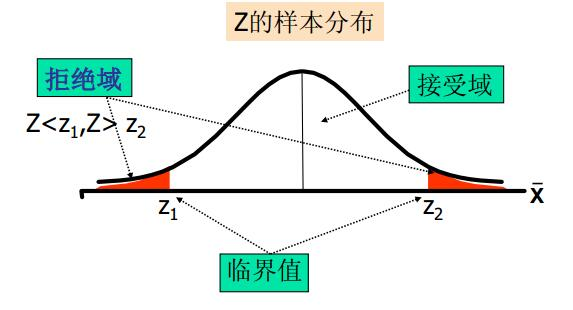
\includegraphics[width=1\linewidth,height=0.35\textheight]{fig/fig12}

\hypertarget{ux7b2cux4e00ux7c7bux9519ux8befux548cux7b2cux4e8cux7c7bux9519ux8bef}{%
\section{第一类错误和第二类错误}\label{ux7b2cux4e00ux7c7bux9519ux8befux548cux7b2cux4e8cux7c7bux9519ux8bef}}

上文介绍了假设检验的过程,但是假设检验过程会不会出现错误呢?其实大家仔细分析拒绝原假设的理由就会发现问题了。通常情况下原假设是小概率事件,但是小概率事件≠0概率事件。小概率事件不是不发生,而是发生概率较小。就像天气预报说明天有99\%的可能不下雨,结果1\%的可能性成为了事实,明天下雨了。因此假设检验中会有两类错误(弃真错误和取伪错误)经常出现。

(1)第一类错误(弃真错误):

\begin{quote}
\begin{itemize}
\tightlist
\item
  原假设为真时拒绝原假设。
\item
  第一类错误的概率为\(\alpha\)(没错,就是它,我们的好朋友,小\(\alpha\)。咳咳咳,就是显著性水平,一般由研究者事先指定,常用的值有0.01, 0.05, 0.10)。
\end{itemize}
\end{quote}

(2)第二类错误(取伪错误):

\begin{quote}
\begin{itemize}
\tightlist
\item
  原假设为假时未拒绝原假设。
\item
  第二类错误的概率记为\(\beta\)。
\end{itemize}
\end{quote}

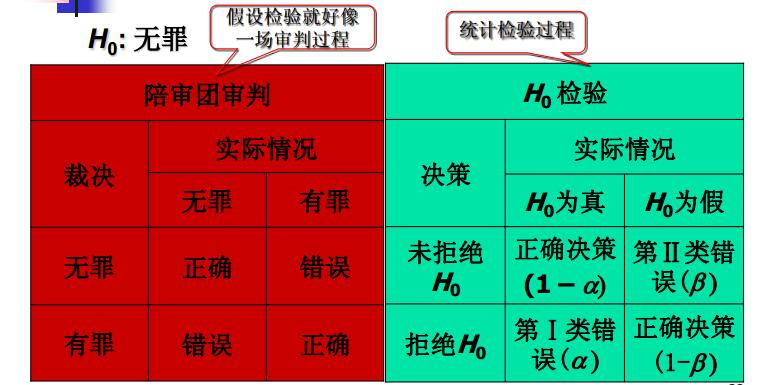
\includegraphics[width=1\linewidth,height=0.35\textheight]{fig/fig13}

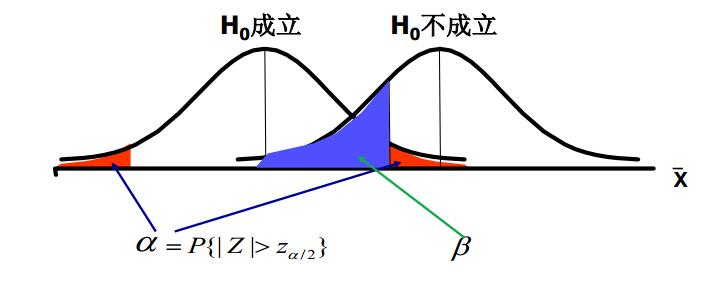
\includegraphics[width=1\linewidth,height=0.35\textheight]{fig/fig14}

\(\alpha\)和\(\beta\)的关系------\(\alpha\)和\(\beta\)的关系就像翘翘板,\(\alpha\)小\(\beta\)就大,\(\alpha\)大\(\beta\)就小。所以两类错误不可能同时发生(第一类只在\(H_0\)为真时发生,第而类只在\(H_0\)为假时发生)。

影响\(\beta\)的因素:
\textgreater{} * 总体参数的真值。
\textgreater{} * 显著性水平\(\alpha\)(当\(\alpha\)减少时增大)。
\textgreater{} * 总体标准差\(\sigma\)(当\(\sigma\)增大时增大)。
\textgreater{} * 样本容量n(当n减少时增大)。

\hypertarget{ux7edfux8ba1ux91cfux4e0eux62d2ux7eddux57df}{%
\section{统计量与拒绝域}\label{ux7edfux8ba1ux91cfux4e0eux62d2ux7eddux57df}}

讲了这么多,但是还没有介绍假设检验的计算过程。假设检验的过程依赖于两个重要数学概念(统计量与拒绝域,前面已经有稍微提到了)。这里再做具体介绍。检验统计量(test statistic)------根据样本观测结果计算得到的,并据以对原假设和备择假设作出决策的某个样本统计量,是对样本估计量的标准化结果(原假设\(H_0\)为真,点估计量的抽样分布)。标准化的检验统计量公式为:标准化的检验统计量=(点估计量-假设值)/点估计量的抽样标准差

显著性水平和拒绝域的三种情况。

\begin{itemize}
\tightlist
\item
  双侧检验:
\end{itemize}

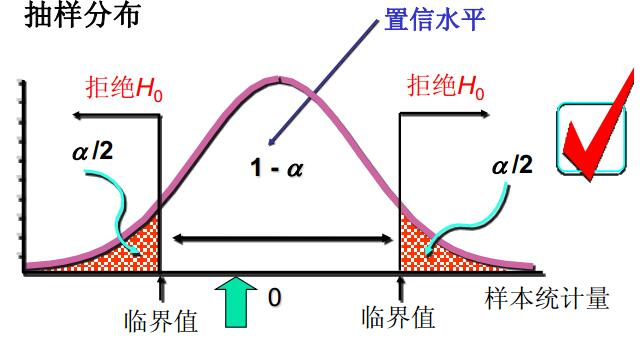
\includegraphics[width=1\linewidth,height=0.35\textheight]{fig/fig15}

\begin{itemize}
\tightlist
\item
  左侧检验:
\end{itemize}

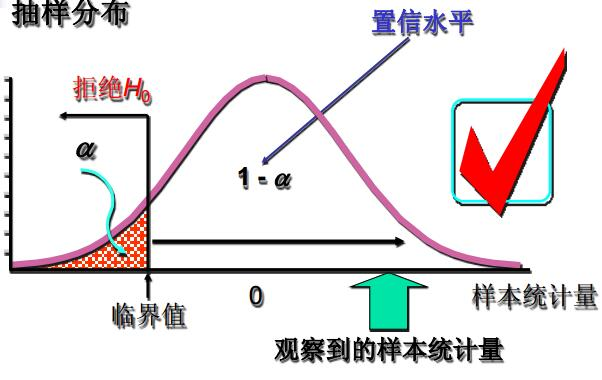
\includegraphics[width=1\linewidth,height=0.35\textheight]{fig/fig16}

\begin{itemize}
\tightlist
\item
  右侧检验:
\end{itemize}

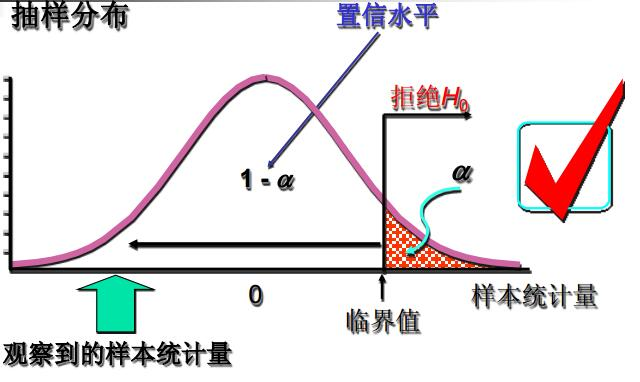
\includegraphics[width=1\linewidth,height=0.35\textheight]{fig/fig17}

统计量落在拒绝域时,我们就可以拒绝原假设。具体如下:

\begin{quote}
\begin{itemize}
\tightlist
\item
  给定显著性水平\(\alpha\),查表得出相应的临界值\(z_{\alpha},z_{\alpha/2},t_{\alpha},t_{\alpha/2},\cdots\)。
\item
  将检验统计量的值与\(\alpha\)水平的临界值进行比较。
\item
  作出决策:双侧检验------\textbar 统计量\textbar{} \textgreater{} 临界值,拒绝\(H_0\);左侧检验------统计量 \textless{} 临界值,拒绝\(H_0\);右侧检验------统计量 \textgreater{} 临界值,拒绝\(H_0\)。
\end{itemize}
\end{quote}

\hypertarget{ux5229ux7528pux503cux8fdbux884cux51b3ux7b56}{%
\section{利用p值进行决策}\label{ux5229ux7528pux503cux8fdbux884cux51b3ux7b56}}

如何利用假设检验解决实际问题?很重要的一个应用是在决策上。就如标题说的,利用p值进行决策。那么什么是p值?p值(p-value):在一个假设检验问题中,拒绝原假设的最小显著性水平。

\begin{quote}
\begin{itemize}
\tightlist
\item
  在原假设为真的条件下,检验统计量的观察值大于或等于其计算值的概率(双侧检验为分布中检验统计量两侧面积的总和;单侧检验为分布中检验统计量相应单侧面积)。
\item
  反映实际观测到的数据与原假设\(H_0\)之间的一致程度。
\item
  被称为观察到的(或实测的)显著性水平。
\item
  决策规则: 若p值\textless{}\(\alpha\), 拒绝\(H_0\)。
\end{itemize}
\end{quote}

\begin{itemize}
\tightlist
\item
  p值法步骤(以大样本均值为例),将样本统计量转换成检验统计量z。
\end{itemize}

\begin{quote}
\begin{itemize}
\tightlist
\item
  计算p值: Z为标准正态分布随机变量(p值=\((\left|Z\right|\ge z)\)(双侧),p值=\((Z\le z)\)(左侧),p值=\((Z\ge z)\)(右侧))
\item
  比较p值和\(\alpha\):
  如果\(\alpha \leq p\)值,拒绝\(H_0\);
  如果\(\alpha<\)p值,不能拒绝\(H_0\)。
\end{itemize}
\end{quote}

\begin{itemize}
\tightlist
\item
  假设检验结论的表述
\end{itemize}

假设检验的目的就在于试图找到拒绝原假设的证据, 而不在于证明什么是正确的。

\begin{quote}
\begin{itemize}
\tightlist
\item
  拒绝原假设时结论是清楚的。
\item
  当不拒绝原假设时------并未给出明确的结论,不能说原假设是正确的, 也不能说它不是正确的。但也未说它不是10。 我们只能说样本提供的证据还不足以推翻原假设。
\end{itemize}
\end{quote}

\begin{itemize}
\tightlist
\item
  假设检验步骤的总结
\end{itemize}

\begin{quote}
\begin{itemize}
\tightlist
\item
  陈述原假设和备择假设。
\item
  从所研究的总体中抽出一个随机样本。
\item
  确定一个适当的检验统计量, 并利用样本数据算出其具体数值。
\item
  确定一个适当的显著性水平, 并计算出其临界值, 指定拒绝域。
\item
  将统计量的值与临界值进行比较, 作出决策------统计量的值落在拒绝域,拒绝\(H_0\),否则不拒绝\(H_0\),也可以直接利用p值作出决策。
\end{itemize}
\end{quote}

\hypertarget{ux4e00ux4e2aux603bux4f53ux53c2ux6570ux7684ux68c0ux9a8c}{%
\section{一个总体参数的检验}\label{ux4e00ux4e2aux603bux4f53ux53c2ux6570ux7684ux68c0ux9a8c}}

前面的理论讲的差不多了,又到了典型总体参数的检验内容的介绍了。依旧是先一个总体参数的检验(总体均值、总体比例、总体方差)。

\begin{itemize}
\tightlist
\item
  总体均值的检验(大样本:\(n\geq30\)),使用z检验统计量:
\end{itemize}

\(\sigma^2\)已知:\(z=\frac{\bar x-\mu_0}{\sigma/\sqrt{n}}\sim N(0,1)\)。

\(\sigma^2\)未知:\(z=\frac{\bar x-\mu_0}{s/\sqrt{n}}\sim N(0,1)\)。

\begin{itemize}
\tightlist
\item
  总体均值的检验(正态总体小样本),检验统计量:
\end{itemize}

\(\sigma^2\)已知:\(z=\frac{\bar x-\mu_0}{\sigma/\sqrt{n}}\sim N(0,1)\)。

\(\sigma^2\)未知:\(t=\frac{\bar x-\mu_0}{s/\sqrt{n}}\sim t(n-1)\)。

\begin{itemize}
\tightlist
\item
  总体比例的检验
\end{itemize}

假定条件:

\begin{quote}
\begin{itemize}
\tightlist
\item
  总体服从二项分布;
\item
  可用正态分布来近似(大样本)。
\end{itemize}
\end{quote}

检验的Z统计量:\(z=\frac{\bar q-p_0}{\sqrt{\frac{p_0(1-p_0)}{n}}}\sim N(0,1)\),\(p_0\)为假设的总体比例。

\begin{itemize}
\tightlist
\item
  总体方差的检验
\end{itemize}

检验一个总体的方差或标准差,假设总体近似服从正态分布,使用\(\chi^2\)分布。检验统计量:

\[\chi^2=\frac{(n-1)s^2}{\sigma_0^2}\sim \chi^2(n-1)\]

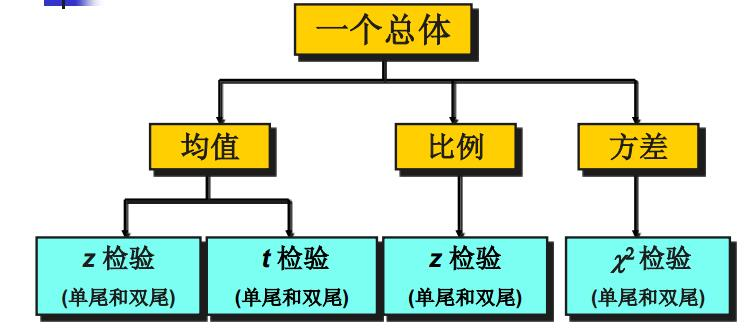
\includegraphics[width=1\linewidth,height=0.35\textheight]{fig/fig18}

这里顺带提下作为统计推断的两大分支的区间估计和假设检验的关系。

\begin{quote}
\begin{itemize}
\tightlist
\item
  过程相似:如果假设均值在95\%的置信区间之外,双边检验将拒绝原假设(显著性水平为5\%)。
\item
  逻辑不同:置信区间------不知道均值多少而要估计它;假设检验: 假定一个均值要看数据是否支持这个假设。
\end{itemize}
\end{quote}

另外还是要谈一谈统计学与实际问题------这里谈的是统计显著性和实际显著性。一个被拒绝的原假设意味着有统计显著性,但未必有实际显著性。这种情况常发生在大样本或精确测量场合,如Kepler的行星运行第一定律:行星轨道是椭圆的,当时吻合程度很好,100年后,仪器更高级、测量更精确,该假设被拒绝,因为行星间交互作用导致摄动。因此不要盲目使用统计显著性。此外,显著性水平\(\alpha\)的选择也是个很关键的问题。一般来说:

\begin{quote}
\begin{itemize}
\tightlist
\item
  \(\alpha\)不宜过小,否则第二类错误概率会较大。
\item
  \(\alpha\)的选择与判断发生错误时要付出的代价大小有关。
\item
  \(\alpha\)的选择是决策问题。
\end{itemize}
\end{quote}

\hypertarget{ux4e24ux4e2aux603bux4f53ux53c2ux6570ux7684ux68c0ux9a8c}{%
\section{两个总体参数的检验}\label{ux4e24ux4e2aux603bux4f53ux53c2ux6570ux7684ux68c0ux9a8c}}

讲完了一个总体参数,照例来讲就两个总体参数(两个总体均值之差,两个总体比例之差,两个总体方差比)。

\begin{itemize}
\tightlist
\item
  独立大样本两总体均值之差检验
\end{itemize}

假定条件:

\begin{quote}
\begin{itemize}
\tightlist
\item
  两个样本是独立的随机样本。
\item
  大样本(\(n_1\ge30\)和\(n_2\ge30\))。
\end{itemize}
\end{quote}

检验统计量:

\(\sigma_1^2,\sigma_2^2\)已知:

\[z=\frac{(\bar x_1-\bar x_2)-(\mu_1-\mu_2)}{\sqrt{\frac{\sigma_1^2}{n_1}+\frac{\sigma_2^2}{n_2}}}\sim N(0,1)\]。

\(\sigma_1^2,\sigma_2^2\)未知:

\[z=\frac{(\bar x_1-\bar x_2)-(\mu_1-\mu_2)}{\sqrt{\frac{s_1^2}{n_1}+\frac{s_2^2}{n_2}}}\sim N(0,1)\]。

\begin{itemize}
\tightlist
\item
  正态总体独立小样本均值之差检验(\(\sigma_1^2,\sigma_2^2\)已知)
\end{itemize}

假定条件:

\begin{quote}
\begin{itemize}
\tightlist
\item
  两个独立的小样本。
\item
  两个总体都是正态分布。
\item
  \(\sigma_1^2,\sigma_2^2\)已知。
\end{itemize}
\end{quote}

检验统计量:

\[z=\frac{(\bar x_1-\bar x_2)-(\mu_1-\mu_2)}{\sqrt{\frac{\sigma_1^2}{n_1}+\frac{\sigma_2^2}{n_2}}}\sim N(0,1)\]。

\begin{itemize}
\tightlist
\item
  正态总体独立小样本均值之差检验(\(\sigma_1^2,\sigma_2^2\)未知但\(\sigma_1^2=\sigma_2^2\))
\end{itemize}

假定条件:

\begin{quote}
\begin{itemize}
\tightlist
\item
  两个独立的小样本。
\item
  两个总体都是正态分布。
\item
  \(\sigma_1^2,\sigma_2^2\)未知但相等,即\(\sigma_1^2=\sigma_2^2\)。
\end{itemize}
\end{quote}

检验统计量:

\[t=\frac{(\bar x_1-\bar x_2)-(\mu_1-\mu_2)}{s_p\sqrt{\frac{1}{n_1}+\frac{1}{n_2}}}\]

其中\(s_p=\frac{(n_1-1)s_1^2+(n_2-1)s_2^2}{n_1+n_2-2}\),自由度:\(n_1+n_2-2\)。

\begin{itemize}
\tightlist
\item
  两个总体均值之差的检验(\(\sigma_1^2,\sigma_2^2\)未知且不相等\(\sigma_1^2\ne\sigma_2^2\))
\end{itemize}

假定条件:

\begin{quote}
\begin{itemize}
\tightlist
\item
  两个总体都是正态分布。
\item
  \(\sigma_1^2,\sigma_2^2\)未知且不相等,即\(\sigma_1^2\ne\sigma_2^2\)。
\item
  样本容量相等,\(n_1=n_2=n\)。
\end{itemize}
\end{quote}

检验统计量:

\[t=\frac{(\bar x_1-\bar x_2)-(\mu_1-\mu_2)}{\sqrt{\frac{s_1^2}{n_1}+\frac{s_2^2}{n_2}}}=\frac{(\bar x_1-\bar x_2)-(\mu_1-\mu_2)}{\sqrt{\frac{s_1^2+s_2^2}{n}}}\]

自由度:\(n_1+n_2-2=2(n-1)\)。

\begin{itemize}
\tightlist
\item
  两个总体均值之差的检验(\(\sigma_1^2,\sigma_2^2\)未知且不相等\(\sigma_1^2\ne\sigma_2^2\))
\end{itemize}

假定条件:

\begin{quote}
\begin{itemize}
\tightlist
\item
  两个总体都是正态分布。
\item
  \(\sigma_1^2,\sigma_2^2\)未知且不相等,即\(\sigma_1^2\ne\sigma_2^2\)。
\item
  样本容量不相等,\(n_1\ne n_2\)。
\end{itemize}
\end{quote}

检验统计量:

\[t=\frac{(\bar x_1-\bar x_2)-(\mu_1-\mu_2)}{\sqrt{\frac{s_1^2}{n_1}+\frac{s_2^2}{n_2}}}\]

自由度:最接近v的整数------\(v=\frac{(\frac{s_1^2}{n_1}+\frac{s_2^2}{n_2})^2}{\frac{(s_1^2/n_1)^2}{n_1-1}+\frac{(s_2^2/n_2)^2}{n_2-1}}\)。

\begin{itemize}
\tightlist
\item
  两个总体均值之差的检验(匹配样本)
\end{itemize}

假定条件:

\begin{quote}
\begin{itemize}
\tightlist
\item
  两个总体配对差值构成的总体服从正态分布。
\item
  配对差是由差值总体中随机抽取的。
\item
  数据配对或匹配(重复测量 (前/后))。
\end{itemize}
\end{quote}

样本差值均值

\[\bar d=\frac{\sum_{i=1}^n d_i}{n_d}\],

样本差值标准差值

\[s_d=\sqrt{\frac{\sum_{i=1}^n(d_i-\bar d)^2}{n_d-1}}\]。

大样本检验统计量:

\[z=\frac{\bar d-d_0}{s_d/\sqrt{n_d}}\sim N(0,1)\]。

小样本检验统计量:

\[t=\frac{\bar d-d_0}{s_d/\sqrt{n_d}}\sim t(n-1)\]。

\begin{itemize}
\tightlist
\item
  两个总体比例之差的检验
\end{itemize}

假定条件:

\begin{quote}
\begin{itemize}
\tightlist
\item
  两个总体都服从二项分布。
\item
  可以用正态分布来近似。
\end{itemize}
\end{quote}

检验统计量:

检验\(H_0:p_1-p_2=0\),

\[z=\frac{\bar p_1-\bar p_2}{\sqrt{\bar p(1-\bar p)(\frac{1}{n_1}+\frac{1}{n_2})}}\],

其中\(\bar p=\frac{x_1+x_2}{n_1+n_2}=\frac{\bar p_1n_1+\bar p_2n_2}{n_1+n_2}\)。

检验\(H_0:p_1-p_2=d_0\),

\[z=\frac{(\bar p_1-\bar p_2)-d_0}{\sqrt{\frac{\bar p_1(1-\bar p_1)}{n_1}+\frac{\bar p_2(1-\bar p_2)}{n_2}}}\]。

\begin{itemize}
\tightlist
\item
  两个总体方差比的检验(F检验)
\end{itemize}

假定条件:

\begin{quote}
\begin{itemize}
\tightlist
\item
  两个总体都服从正态分布。
\item
  两个独立的随机样本。
\end{itemize}
\end{quote}

检验统计量:

\[F=\frac{s_1^2}{s_2^2}\sim F(n_1-1,n_2-1)\]

或

\[F=\frac{s_2^2}{s_1^2}\sim F(n_2-1,n_1-1)\]。

最后的总结就是如下图。

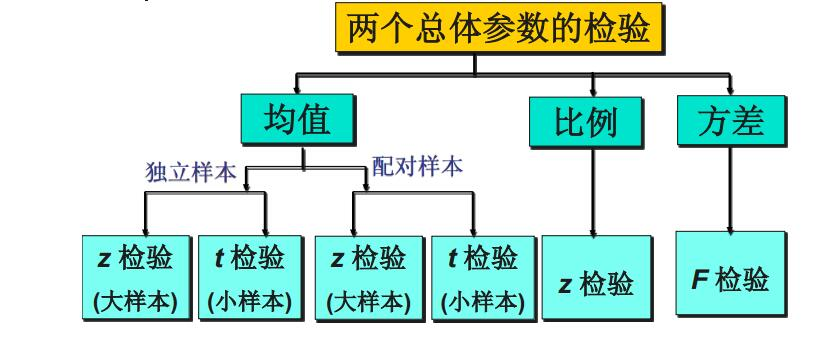
\includegraphics[width=1\linewidth,height=0.35\textheight]{fig/fig19}

最后的最后,回到开头提的问题------雄安新区。该问题其实是两个总体参数的检验问题------两个总体均值之差的问题(两个总体分别是批复前的房价和批复后的房价)。所以如果要讨论该问题,可以考虑从批复前后的房价,抽取配对大样本或小样本(楼盘房价)进行假设检验,这样我们就能在统计学上证明这件事对雄安房价的显著影响啦。本篇涉及的R语言内容较少,还是老规矩,放到后面的第14章去讨论。

\hypertarget{goodness}{%
\chapter{Goodness of Fit}\label{goodness}}

本篇是第七章,内容是拟合优度检验。

\hypertarget{ux591aux9879ux5206ux5e03}{%
\section{多项分布}\label{ux591aux9879ux5206ux5e03}}

拟合优度检验的第一个应用是关于多项总体。那么多项总体(或者多项分布)是什么呢?

\begin{quote}
\begin{itemize}
\tightlist
\item
  多项分布是二项分布的推广。
\item
  总体被分为几个互不相交的类别。
\item
  多项分布假设:每次试验有且仅有一个结果发生;每次试验独立;每次试验概率不变。
\end{itemize}
\end{quote}

拟合优度检验-多项总体步骤,将所观测到的数据与理论上的期望值进行比较。步骤:

\begin{quote}
\begin{itemize}
\tightlist
\item
  1.计算每一类实际观测到的频次\(f_i\);
\item
  2.计算每一类理论上的期望频次\(e_i\);
\item
  3.计算 Chi-square 统计量------\(\chi^2=\sum(f_i-e_i)^2/e_i\)。其中自由度 (df) = k-1, k 是多项总体的类别数。
\end{itemize}
\end{quote}

拟合优度检验用于多项总体检验没有直接的函数,这里用R语言的自编函数实现,体会下具体的算法(当然感觉自己写的略复杂)。代码依旧是后面放出,函数具体使用说明也会附上。

\hypertarget{ux72ecux7acbux6027}{%
\section{独立性}\label{ux72ecux7acbux6027}}

依旧是从问题出发------性别与购物频率是否有关系。独立性检验------该统计方法常用于检验两个分类变量是否有关系。那么首先要提到两个概念------独立事件和非独立事件(independent and dependent events)。

\begin{quote}
\begin{itemize}
\tightlist
\item
  独立事件------一个事物发生不会对其他事物发生概率造成影响。
\item
  非独立事件------一个事物发生会影响其他事物发生概率。
\end{itemize}
\end{quote}

接着统计学构建出了一个表来进行独立性检验。这就是联立表(Contingency Tables)。

\begin{quote}
\begin{itemize}
\tightlist
\item
  解决多总体比例问题。
\item
  之前通常用两个或两个以上特征来对样本观测值分类。
\item
  也被称为交叉表。
\end{itemize}
\end{quote}

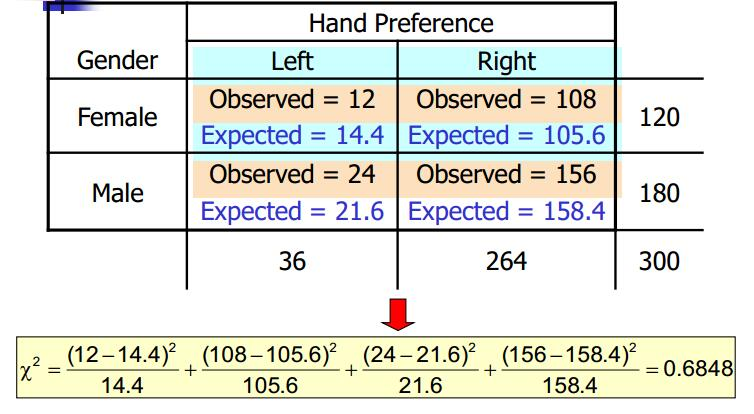
\includegraphics[width=1\linewidth,height=0.35\textheight]{fig/fig20}

一般在R中,使用Table函数即可生成两个特征(分类变量)的联立表,xtabs则是根据公式创立联立表,prop.table则可以直接计算出比例。联立表如何做独立性检验呢?首先提出假设(这里不详述,相信大家应该懂怎么建立了),接着计算期望的联立表每个单元格的期望频次。

\[e_{ij}=\frac{(i^{th} Rowtotal)(j^{th} Columtotal)}{Total SampleSize}\]。

接着就可以对比实际频次和期望频次,然后我们用卡方(chi-square)统计量进行检验。

\[\chi^2=\sum_{i=1}^n\sum_{j=1}^m\frac{(f_{ij}-e_{ij})^2}{e_{ij}} with, df=(n-1)(m-1)\]。

n为行数,m为列数,\(f_{ij},e_{ij}\)分别为第i行和第j列的\(cell_{ij}\)实际频次和期望频次。当然这个方法也可以用来检验顺序变量和分类变量。方法类似,这里不赘述。

\hypertarget{ux6982ux7387ux5206ux5e03}{%
\section{概率分布}\label{ux6982ux7387ux5206ux5e03}}

拟合优度检验的最重要的应用其实是探测一个数据具体的概率分布。当然探测数据分布的第一方式------是可见即可得的可视化。主要包括前面提到过的直方图和QQ图。QQ图------Quantile-Quantile Plots(分位数图):

\begin{quote}
\begin{itemize}
\tightlist
\item
  适用于小数据集。
\item
  猜测分布的基础方法。
\item
  用来绘制QQ图的数据必须落在该分布内。
\item
  如果散点图接近直线,说明数据分布接近正态分布。
\end{itemize}
\end{quote}

这里给出绘制QQ图的原理:

\begin{quote}
\begin{itemize}
\tightlist
\item
  对样本容量为N的样本数据按照升序排序。
\item
  计算从1到N排序的百分比。
\item
  从百分位数得分的关系找到中心分数。
\item
  找到对应于中心分数的z值(标准正态分布)。
\item
  绘制对应z值的观测点数据。
\end{itemize}
\end{quote}

接着用R语言实现。

\begin{Shaded}
\begin{Highlighting}[]
\CommentTok{#QQ plot}
\CommentTok{#generation of random number that fall in normal distribution}
\NormalTok{a<-}\KeywordTok{rnorm}\NormalTok{(}\DecValTok{200}\NormalTok{,}\DecValTok{0}\NormalTok{,}\DecValTok{1}\NormalTok{)}

\CommentTok{#plot}
\KeywordTok{qqnorm}\NormalTok{(a)}
\KeywordTok{qqline}\NormalTok{(a,}\DataTypeTok{col=}\StringTok{"red"}\NormalTok{)}
\end{Highlighting}
\end{Shaded}

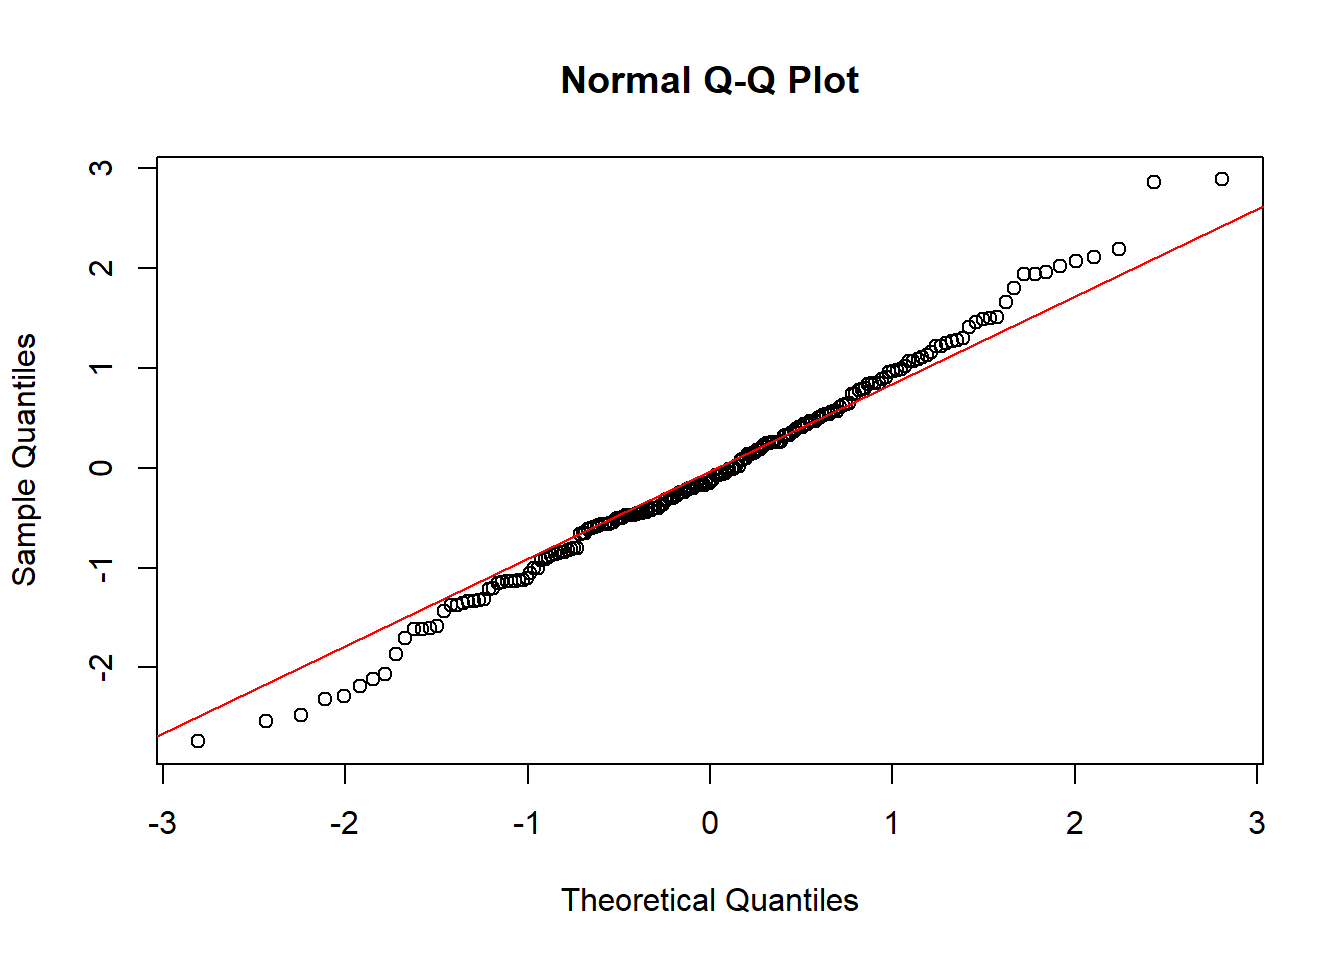
\includegraphics[width=1\linewidth,height=0.4\textheight]{bookdown_files/figure-latex/unnamed-chunk-35-1}

除了QQ图之外,另外一类方法就是通过统计方法------拟合优度检验来探测数据是否正态分布。以正态分布为例。过程:

\begin{quote}
\begin{itemize}
\tightlist
\item
  获取样本数据。
\item
  将样本结果分组(单元格)。
\item
  比较实际与预期值。
\end{itemize}
\end{quote}

统计量如下:
\[\chi^2=\sum_{i=1}^k\frac{(f_i-ei-)^2}{e_i}\]。

R语言中可以用chisp.test函数进行正态分布测验。

此外对于有某种特定分布的非正态数据可以通过数学变换转变为正态分布数据。常用的一般包括:

\begin{quote}
\begin{itemize}
\tightlist
\item
  对数变换。
\item
  开方变换。
\item
  指数或平方变换。
\end{itemize}
\end{quote}

这里的数学变换需要根据大家实际研究需求决定。

\hypertarget{ANOVA}{%
\chapter{ANOVA}\label{ANOVA}}

本篇是第八章,内容是方差分析。方差分析是很多实验的基础以及很重要的分析手段,这一章内容相比较而言比较多。

\hypertarget{ux65b9ux5deeux5206ux6790ux7684ux5f15ux8bba}{%
\section{方差分析的引论}\label{ux65b9ux5deeux5206ux6790ux7684ux5f15ux8bba}}

方差分析其实对我们来说并不陌生,因为大学搞生态的那群同学,实验中无数次出现了单方差因素分析的方法。那么方差分析究竟是什么呢?从引论来说,我们举个跟地学领域相关的例子。不同地貌对土壤有机质是否有影响?简单地说方差分析实质适合分析的是一系列数值型数据存在某个属性(也可以是某些),然后这个属性可以按照一定的规则分成几个类别(或者叫水平),我们想了解的就是,不同类别或者不同水平的这个数值是否存在显著性差异。简单的理解,它是处理分类型数据的。这里需要跟上一章提到的拟合优度检验、后面讲到的回归分析做些区别,拟合优度检验通常是分析两个分类变量的关系,回归分析则分析的是一个数值型变量(或多个数值型变量)对一个数值型变量的影响(或者说二者的关系)。而方差分析则是分析一个分类变量(或多个分类变量)对于一个数值变量的影响(或者说二者的关系)。

这里给出一些定义和术语(不喜好数学的同学可以跳过,但请记住我上面的内容):

\textbf{方差分析(Analysis of Variance,ANOVA)}

研究分类型自变量对数值型因变量的影响。

\begin{quote}
\begin{itemize}
\tightlist
\item
  一个或多个分类型自变量:两个或多个 (k 个) 处理或分类
\item
  一个数值型因变量
\end{itemize}
\end{quote}

通过检验多个总体均值是否相等来判断是否有显著影响

\begin{quote}
\begin{itemize}
\tightlist
\item
  通过分析数据的误差判断各总体均值是否相等
\end{itemize}
\end{quote}

有单因子方差分析和双因子方差分析

\begin{quote}
\begin{itemize}
\tightlist
\item
  单因子方差分析:涉及一个分类型自变量
\item
  双因子方差分析:涉及两个分类型自变量
\end{itemize}
\end{quote}

方差分析 vs 假设检验

(1)假设检验:一次只能研究两个样本

\begin{quote}
\begin{itemize}
\tightlist
\item
  需要比较的次数随因子的数量增多而增多;
\item
  第一类错误发生的可能性增大。
\end{itemize}
\end{quote}

(2)方差分析:同时分析多个样本

\begin{quote}
\begin{itemize}
\tightlist
\item
  提高检验效率;
\item
  将所有信息结合在一起, 增加了分析的可靠性。
\end{itemize}
\end{quote}

\hypertarget{ux65b9ux5deeux5206ux6790ux7684ux90e8ux5206ux6982ux5ff5}{%
\subsection{方差分析的部分概念}\label{ux65b9ux5deeux5206ux6790ux7684ux90e8ux5206ux6982ux5ff5}}

\begin{quote}
\begin{itemize}
\tightlist
\item
  因子或因素 (factor)------所要检验的对象,要分析行业对投诉次数是否有影响, 行业是要检验的因子或因素。
\item
  水平或处理(treatment):因子的不同表现,零售业、 旅游业、 航空公司、 家电制造业就是因子的处理。
\item
  观察值:在每个因子处理下得到的样本数据,每个行业被投诉的次数就是观察值。
\item
  试验:涉及一个因子多水平, 可称为单因子多处理的试验。
\item
  总体:因子的每一个处理看作是一个总体。
\item
  样本数据:观察值可以看作是从着多个总体中抽取的样本数据
\end{itemize}
\end{quote}

也就是说分类变量是因子或因素,而分的类别就可以称为水平或处理,观察值则是数值型变量。试验就是就是分类的过程,总体其实就是水平,样本数据就是观测值。

接下来讲讲方差分析的基本思想和原理。

\hypertarget{ux65b9ux5deeux5206ux6790ux7684ux57faux672cux601dux60f3ux548cux539fux7406}{%
\subsection{方差分析的基本思想和原理}\label{ux65b9ux5deeux5206ux6790ux7684ux57faux672cux601dux60f3ux548cux539fux7406}}

方差分析的基本思想和原理基于两类误差。也就是随机误差和系统误差。

\begin{quote}
\begin{itemize}
\tightlist
\item
  \textbf{随机误差}------因子的同一处理(总体)下, 样本各观察值之间的差异,这种差异可以看成是随机因素的影响, 称为随机误差。
\item
  \textbf{系统误差}------因子的不同处理(不同总体)下,各观察值之间的差异,这种差异可能是由于抽样的随机性所造成的,也可能是由于行业本身所造成的,后者所形成的误差是由系统性因素造成的,称为系统误差。
\end{itemize}
\end{quote}

所以方差分析的实质是------比较两类误差,以检验均值是否相等;比较的基础是方差比;如果系统(处理)误差明显地不同于随机误差,则均值就是不相等的;反之,均值就是相等的。这里数据的误差用平方和(sum of squares)表示。

\begin{quote}
\begin{itemize}
\tightlist
\item
  \textbf{组内平方和(within groups)}------因子的同一处理(同一个总体)下样本数据的平方和。组内平方和只包含随机误差。
\item
  \textbf{组间平方和(between groups)}------因子的不同处理(不同总体)下各样本之间的平方和。组间平方和既包括随机误差, 也包括系统误差。
\end{itemize}
\end{quote}

所以若原假设成立, 组间平方和与组内平方和经过平均后的数值就应该很接近, 它们的比值就会接近1。

\begin{quote}
\begin{itemize}
\tightlist
\item
  若原假设不成立, 组间平方和平均后的数值就会大于组内平方和平均后的数值, 它们之间的比值就会大于1。
\item
  当这个比值大到某种程度时, 就可以说不同处理之间存在着显著差异, 也就是自变量对因变量有影响。
\end{itemize}
\end{quote}

\hypertarget{ux65b9ux5deeux5206ux6790ux7684ux57faux672cux5047ux5b9a}{%
\subsection{方差分析的基本假定}\label{ux65b9ux5deeux5206ux6790ux7684ux57faux672cux5047ux5b9a}}

(1)每个总体都应服从正态分布:对于因子的每一个处理, 其观察值是来自服从正态分布总体的简单随机样本。

(2)各个总体的方差必须相同:各组观察数据是从具有相同方差的总体中抽取的。

(3)观察值是独立的。

(4)在上述假定条件下, 判断行业对投诉次数是否有显著影响, 实际上也就是检验具有同方差的四个正态总体的均值是否相等。

(5)如果四个总体的均值相等, 可以期望四个样本的均值也会很接近:四个样本的均值越接近,推断四个总体均值相等的证据也就越充分;样本均值越不同, 推断总体均值不同的证据就越充分。

这里要注意的是,往往很多人做统计的时候往往不考虑前提和假设,这是一个错误。经典统计学中很多模型都有严密的数学推导和前提假设,就笔者从事的地学领域里其实有很多现象不是太遵循经典统计学的前提,由此也衍生出了空间统计学理论,所以在做统计研究时需要考量自己数据的特征,了解统计学与模型的基本前提与假设。

原假设:\(H_0:\mu_1=\mu_2=\mu_3=\cdots=\mu_n\)

\begin{quote}
\begin{itemize}
\tightlist
\item
  n个水平被投诉次数的均值都相等;
\item
  意味着每个样本都来自均值为\(\mu\)、方差为\(\sigma^2\)的同一正态总体。
\end{itemize}
\end{quote}

若备择假设成立,即\(H_1:\mu_i(i=1,2,3,\cdots,n)\)不全相等

\begin{quote}
\begin{itemize}
\tightlist
\item
  至少有一个总体的均值是不同的;
\item
  样本分别来自均值不同的多个个正态总体。
\end{itemize}
\end{quote}

\hypertarget{ux5355ux56e0ux5b50ux65b9ux5deeux5206ux6790one-way-anova}{%
\section{单因子方差分析(One-way ANOVA)}\label{ux5355ux56e0ux5b50ux65b9ux5deeux5206ux6790one-way-anova}}

从这章开始后面的部分基本是典型数据分析,故我会渗透更多的数据分析的一些经验和理念。在这里因为要正式进入方差分析的具体内容里,所以我想谈的一点是我曾经说过的一句话------编程先学数据结构。数据结构的重要性可以参加下面的知乎。

\begin{quote}
\begin{itemize}
\tightlist
\item
  \url{https://www.zhihu.com/question/29587605}
\end{itemize}
\end{quote}

当然对于R或是其他数据处理语言来说,我觉得最关键的是你在使用分析数据(调用各种包)时需要了解你所调用的包或者函数处理的是什么样的数据(你要把数据处理成你的函数可以读的形式)。当然这是题外话,还是回到标题的单因子方差分析。如果一个试验中,只有一个因子在变,而其它因素保持不变,称此试验为单因子试验(只涉及一个分类型自变量)。那么它的数据结构如下所示:

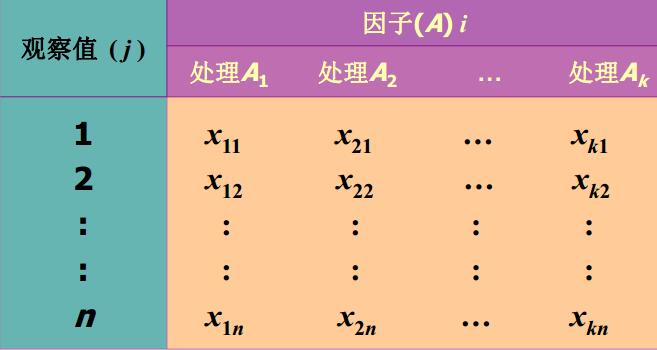
\includegraphics[width=1\linewidth,height=0.35\textheight]{fig/fig21}

当然事实上在分析的时候,个人觉得R和其他数据所能读取的数据结构或者说组织方式还是2列的变量(数值型变量与分类变量)。分析步骤则是统计学的经典三部曲:

\begin{quote}
\begin{itemize}
\tightlist
\item
  提出假设;
\item
  构造检验统计量;
\item
  统计决策。
\end{itemize}
\end{quote}

假设的提法在前面已经提过了。

\(H_0:\mu_1=\mu_2=\mu_3=\cdots=\mu_n\)(自变量对因变量没有显著影响)。

\(H_1:\mu_1,\mu_2,\mu_3,\cdots,\mu_n\)不全相等(自变量对因变量有显著影响)。

构造统计量需要计算:(1)处理的均值;(2)全部观察值的总均值;(3)平方和;(4)均方(MS)。(接下来是公式大全,公式恐惧症者请跳过)

\textbf{(1)处理的均值}

假定从第i个总体中抽取一个容量为\(n_i\)的简单随机样本, 第i个总体的样本均值为该样本的全部观察值总和除以观察值的个数。

\[\bar x_i=\frac{\sum_{j=1}^nx_{ij}}{n_i} (i=1,2,\cdots,k)\]

式中: \(n_i\)为第 i 个总体的样本观察值个数,\(x_{ij}\)为第i个总体的第j个观察值。

\textbf{(2)全部观察值的总均值}

全部观察值的总和除以观察值的总个数。

\[\bar x'=\frac{\sum_{i=1}^k\sum_{j=1}^nx_{ij}}{n}=\frac{\sum_{i=1}^kn_i\bar x_i}{n}\]

\textbf{(3)平方和}

方差分析需要计算三个平方和。
\textgreater{} * 总平方和 (Sum of Squares for Total),SST。全部观察值与总平均值的离差平方和,反映全部观察值的离散状况。\(SST=\sum_{i=1}^k\sum_{j=1}^n(x_{ij}-\bar x')^2\)
\textgreater{} * 处理平方和 (Sum of Squares due to Treatment), SSTR,又叫组间平方和。各组平均值与总平均值的离差平方和,反映各总体的样本均值之间的差异程度,又称处理平方和或组间平方和,该平方和既包括随机误差, 也包括系统误差。\(SSTR= \sum_{i=1}^k\sum_{j=1}^n(\bar x_i-\bar x')^2=\Sigma_{i=1}^kn_i(\bar x_i-\bar x')^2\)。
\textgreater{} * 误差平方和 (Sum of Squares due to Error),SSE,又叫组内平方和。每个处理或组的各样本数据与其组平均值的离差平方和,反映每个样本各观察值的离散状况,又称组内平
方和或残差平方和,该平方和反映的是随机误差的大小。\(SSE=\sum_{i=1}^k\sum_{j=1}^n(x_ij-\bar x_i)^2\)。

实际上,SST=SSTR+SSE。SST反映全部数据总的误差程度; SSE反映随机误差的大小;SSTR反映随机误差和系统误差的大小。如果原假设成立,则表明没有系统误差,处理平方和SSTR除以自由度后的均方与误差平方和SSE和除以自由度后的均方差异就不会太大;如果处理均方显著地大于误差均方,说明各处理(总体)之间的差异不仅有随机误差, 还有系统误差。判断因子的处理是否对其观察值有影响,实际上就是比较处理均方与误差均方之间差异的大小。

\textbf{(4)均方------构建检验统计量}

各平方和的大小与观察值的多少有关, 为消除观察值多少对平方和大小的影响, 需要将其平均, 这就是均方,也称为方差。计算方法是用平方和除以相应的自由度,三个平方和对应的自由度分别是: SST 的自由度为n-1,其中n为全部观察值的个数,SSTR的自由度为k-1, 其中k为因子处理(总体)的个数,SSE 的自由度为n-k。

处理均方:SSTR的均方, 记为MSTR, 计算公式为:

\[MSTR=\frac{SSTR}{k-1}\]

误差均方:SSE的均方,记为MSE, 计算公式为:

\[MSE=\frac{SSE}{n-k}\]

计算检验统计量F:

将MSTR和MSE进行对比, 即得到所需要的检验统计量F,当\(H_0\)为真时, 二者的比值服从分子自由度为k-1、分母自由度为n-k的F分布, 即

\[F=\frac{MSTR}{MSE}\sim(k-1,n-k)\]

最后是统计决策将统计量的值F与给定的显著性水平\(\alpha\)的临界值\(F_\alpha\)进行比较,作出对原假设\(H_0\)的决策。

\begin{quote}
\begin{itemize}
\tightlist
\item
  根据给定的显著性水平\(\alpha\), 在F分布表中查找与第一自由度\(df_1=k-1\)、 第二自由度\[df_2=n-k\] 相应的临界值\(F_\alpha\)。
\item
  若F\textgreater{}\(F_\alpha\),则拒绝原假设\(H_0\),表明均值之间的差异是显著的,所检验的因子对观察值有显著影响。
\item
  若F\textless{}\(F_\alpha\),则不能拒绝原假设\(H_0\), 无证据支持表明所检验的因子对观察值有显著影响。
\end{itemize}
\end{quote}

对前面的三部曲做一个进一步的总结:

(1)提出假设;

(2)构造检验统计量(均值:全部观察值的总均值、处理的均值;平方和:总平方和SST,处理平方和SSTR,误差平方和SSE;均方:处理均方MSTR,误差均方MSE;均方比:MSTR/MSE\textasciitilde F分布);

(3) 统计决策。

在R语言中,方差分析函数较为简单,具体应用后面再说。value为观察值,factor为因素。

\begin{Shaded}
\begin{Highlighting}[]
\NormalTok{a.aov<-}\KeywordTok{aov}\NormalTok{(value}\OperatorTok{~}\NormalTok{factor,}\DataTypeTok{data=}\NormalTok{a)}
\KeywordTok{summary}\NormalTok{(a.aov)}
\end{Highlighting}
\end{Shaded}

\begin{longtable}[]{@{}lcccr@{}}
\toprule
误差来源(方差来源) & 平方和(SS) & 自由度(df) & 均方(MS) & F\tabularnewline
\midrule
\endhead
组间(处理) & SSTR & k-1 & MSTR=SSTR/(k-1) & MSTR/MSE\tabularnewline
组内(误差) & SSE & n-k & MSE=SSE/(n-k) &\tabularnewline
总计(合计) & SST & n-1 & &\tabularnewline
\bottomrule
\end{longtable}

当然仅仅证明有显著性差异,可能还不能满足我们的需求,所以需要测度方差分析的关系强度。

\textbf{关系强度的测量}

拒绝原假设表明因子(自变量)与观测值之间有关系,而处理平方和(SSTR)度量了自变量(行业)对因变量(投诉次数)的影响效应。

\begin{quote}
\begin{itemize}
\tightlist
\item
  当处理平方和比误差平方和(SSE)大, 而且大到一定程度时, 就意味着两个变量之间的关系显著, 大得越多, 表明它们之间的关系就越强。 反之, 就意味着两个变量之间的关系不显著, 小得越多, 表明它们之间的关系就越弱。
\end{itemize}
\end{quote}

变量间关系的强度用处理平方和(SSTR)及误差平方和(SSE)占总平方和(SST)的比例大小来反映。处理平方和占总平方和的比例记为\(R^2\) ,即\(R^2=\frac{SSTR}{SST}\)(处理平方和)/(总平方和)。其平方根R就可以用来测量两个变量之间的关系强度。

\hypertarget{ux65b9ux5deeux5206ux6790ux4e2dux7684ux591aux91cdux6bd4ux8f83}{%
\section{方差分析中的多重比较}\label{ux65b9ux5deeux5206ux6790ux4e2dux7684ux591aux91cdux6bd4ux8f83}}

多重比较(multiple comparison procedures)------通过对总体均值之间的配对比较来进一步检验到底哪些均值之间存在差异。

\begin{quote}
\begin{itemize}
\tightlist
\item
  可采用Fisher提出的最小显著差异方法, 简写为LSD-least significant difference。LSD方法是对检验两个总体均值是否相等的t检验方法的总体方差估计加以修正( 用MSE来代替) 而得到的。
\end{itemize}
\end{quote}

方差分析中的多重比较分析步骤

(1)提出假设:\(H_0: \mu_i=\mu_j )\)(第i个总体的均值等于第j个总体的均值,\(H_1:\mu_i\neq\mu_j\)(第i个总体的均值不等于第j个总体的均值);

(2)计算检验的统计量: \(\bar x_i-\bar x_j\);

(3)计算LSD,t分布的自由度为n-k(MSE的自由度为n-k)。\(LSD=t_{\alpha/2}\sqrt{MSE(\frac{1}{n_i}+\frac{1}{n_j})}\)

(4)决策:若\(\vert {\bar x_i-\bar x_j} \vert > LSD\),拒绝\(H_0\);若\(\vert {\bar x_i-\bar x_j} \vert < LSD\),不拒绝\(H_0\)。

\hypertarget{ux53ccux56e0ux5b50ux65b9ux5deeux5206ux6790two-way-anova}{%
\section{双因子方差分析(Two-way ANOVA)}\label{ux53ccux56e0ux5b50ux65b9ux5deeux5206ux6790two-way-anova}}

前面介绍完了单因子方差分析,但是当我们的因子大于一个的时候,我们又该怎么分析呢?同样抛个样例问题出来。
假设现在我们想了解北京城市人口空间分布是否受不同环路(一环、二环、三环乃至四、五、六环)或新老城区的显著影响。所以该问题是一个典型的双因子问题,可以拆分为如下的情况:

\begin{longtable}[]{@{}lcr@{}}
\toprule
因子 & 新城区 & 老城区\tabularnewline
\midrule
\endhead
一环 & 人口 & 人口\tabularnewline
二环 & 人口 & 人口\tabularnewline
三环 & 人口 & 人口\tabularnewline
\bottomrule
\end{longtable}

对于该问题我们可以考虑用单因子方差分析来解决------即通过考虑两个因子间所有的组合来分析是否有显著影响。(二环+新城区,二环+老城区,三环+新城区,\ldots\ldots,六环+老城区)通过这样组合来得到最后的单因子水平。但是这样处理的问题是,我们无法了解到底是新老城区的因素影响了人口的空间分布,或者是不同的环路影响了人口的空间分布,亦或是二者共同影响。所以我们需要新的方法来分析。这就是题目所述的双因子方差分析。

\hypertarget{ux53ccux56e0ux5b50ux65b9ux5deeux5206ux6790ux7684ux57faux672cux5047ux5b9a}{%
\subsection{双因子方差分析的基本假定}\label{ux53ccux56e0ux5b50ux65b9ux5deeux5206ux6790ux7684ux57faux672cux5047ux5b9a}}

(1) 每个总体都服从正态分布(对于因素的每一个水平, 其观察值是来自正态分布总体的简单随机样本)。

(2) 各个总体的方差必须相同(对于各组观察数据, 是从具有相同方差的总体中抽取的)。

(3) 观察值是独立的。

双因子方差分析实质是分析两个因素(行因素Row和列因素Column)对试验结果的影响。如果两个因素对试验结果的影响是相互独立的,分别判断行因素和列因素对试验数据的影响, 这时的双因素方差分析称为\textbf{无交互作用的双因素方差分析}或\textbf{无重复双因素方差分析}(Two-factor without replication)。如果除了行因素和列因素对试验数据的单独影响外,两个因素的搭配还会对结果产生一种新的影响, 这时的双因素方差分析称为\textbf{有交互作用的双因素方差分析}或\textbf{可重复双因素方差分析} (Two-factor with replication )。

\hypertarget{ux65e0ux4ea4ux4e92ux4f5cux7528ux53ccux56e0ux5b50ux65b9ux5deeux5206ux6790}{%
\subsection{无交互作用双因子方差分析}\label{ux65e0ux4ea4ux4e92ux4f5cux7528ux53ccux56e0ux5b50ux65b9ux5deeux5206ux6790}}

如果在一项试验中,有两个因子在变,而其余因子保持不变,则称之为双因子试验。

\begin{quote}
\begin{itemize}
\tightlist
\item
  设因子A有a个水平\(A_1,A_2,\cdots,A_a\),因子B有b个水平\(B_1,B_2,\cdots,B_b\),每组因子组合进行1次试验,其结果为\(x_{ij},x_{ij}\sim N(\mu_{ij},\sigma^2)\),现在要研究它们对因变量X的影响。
\end{itemize}
\end{quote}

\textbf{(1)无交互作用双因子方差分析:模型}

\[X_{ij}=\mu+\alpha_i+\beta_j+\varepsilon_{ij}\]

这里\(\varepsilon_{ij}\sim iid,N(0,\sigma^2)\)

\textbf{(2)无交互作用双因子方差分析:假设}

因子A

原假设:\(H_0:\alpha_1= \alpha_2=\cdots= \alpha_a=0\)

备择假设:\(H_1\):至少一个\(\alpha_i\)不等于0

因子B

原假设:\(H_0: \beta_1 = \beta_2 =\cdots= \beta_b=0\)

备择假设:\(H_1\):至少一个\(\beta_i\)不等于0

\textbf{(3)计算步骤(公式大全)}
\textgreater{} * 均方:

\(\bar x_{i.}\)是A因素的第i个水平下各观察值的平均值

\[\bar x_{i.}=\frac{\sum_{j=1}^bx_{ij}}{b}(i=1,2,\cdots,a)\]

\(\bar x_{.j}\)是B因素的第j个水平下各观察值的平均值

\[\bar x_{.j}=\frac{\sum_{i=1}^ax_{ij}}{a}(i=1,2,\cdots,b)\]

\(\bar x'\)是B因素的第j个水平下各观察值的平均值

\[\bar x'=\frac{\sum_{i=1}^a\sum_{j=1}^bx_{ij}}{ab}\]

\begin{quote}
\begin{itemize}
\tightlist
\item
  平方和:
\end{itemize}
\end{quote}

\[SST=\sum_{i=1}^a\sum_{j=1}^b(x_{ij}-\bar x')^2\]

\[SSA=b\sum_{i=1}^a(x_{i.}-\bar x')^2\]

\[SSB=a\sum_{j=1}^b(x_{.j}-\bar x')^2\]

\[SSE=\sum_{i=1}^a\sum_{j=1}^b(x_{ij}-x_{i.}-x_{.j}+\bar x')^2\]

\[SST=SSA+SSB+SSE\]

\begin{quote}
\begin{itemize}
\tightlist
\item
  计算均方(MS)构造检验统计量:误差平方和除以相应的自由度
\end{itemize}
\end{quote}

四个平方和的自由度分别是:总离差平方和SST的自由度为 ab-1;A因素的离差平方和SSA的自由度为 a-1;
B因素的离差平方和SSB的自由度为 b-1;随机误差平方和SSE的自由度为 (a-1)×(b-1)。

A因素的均方,记为MSA,计算公式为:

\[MSA=\frac{SSA}{a-1}\]

B因素的均方,记为MSB,计算公式为:

\[MSB=\frac{SSB}{b-1}\]

随机误差项的均方,记为MSE,计算公式为:

\[MSE=\frac{SSE}{(a-1)(b-1)}\]

\begin{quote}
\begin{itemize}
\tightlist
\item
  计算检验统计量(F)
\end{itemize}
\end{quote}

检验行因素的统计量

\[F_A=\frac{MSA}{MSE}\sim F(a-1,(a-1)(b-1))\]

检验列因素的统计量

\[F_B=\frac{MSB}{MSE}\sim F(b-1,(a-1)(b-1))\]

\begin{quote}
\begin{itemize}
\tightlist
\item
  统计决策
\end{itemize}
\end{quote}

将统计量的值F与给定的显著性水平\(\alpha\)的临界值\(F_\alpha\)进行比较,作出对原假设\(H_0\)的决策:根据给定的显著性水平a在F分布表中查找相应的临界值\(F_\alpha\);若\(F_A>F_\alpha\),则拒绝原假设,表明均值之间的差异是显著的, 即所检验的A因素对观察值有显著影响;若\(F_A>F_\alpha\),则拒绝原假设,表明均值之间有显著差异,即所检验的B因素对观察值有显著影响。

\begin{longtable}[]{@{}lcccr@{}}
\toprule
误差来源(方差来源) & 平方和 & 自由度 & 均方 & F\tabularnewline
\midrule
\endhead
因子A & SSA & a-1 & MSA=SSA/(a-1) & MSA/MSE\tabularnewline
因子B & SSB & b-1 & MSB=SSB/(b-1) & MSB/MSE\tabularnewline
误差 & SSE & (a-1)(b-1) & MSE=SSE/(a-1)(b-1)) &\tabularnewline
总计 & SST & ab-1 & &\tabularnewline
\bottomrule
\end{longtable}

\hypertarget{ux6709ux4ea4ux4e92ux4f5cux7528ux53ccux56e0ux5b50ux65b9ux5deeux5206ux6790}{%
\subsection{有交互作用双因子方差分析}\label{ux6709ux4ea4ux4e92ux4f5cux7528ux53ccux56e0ux5b50ux65b9ux5deeux5206ux6790}}

除了上面的无交互作用双因子方差分析之外,可能存在的一种情况就是二者同时作用,这就是有交互作用的双因子方差分析。
即(\(A_i,B_j\))下作了r个试验,所得结果记作\(x_{ijk},x_{ijk}\)服从\(N(\mu_{ij},\sigma^2),i=1,\cdots,a,j=1,\cdots,b,k=1,\cdots,r\)。且相互独立。

\textbf{(1)有交互作用双因子方差分析:模型}

\[X_{ijk}=\mu+\alpha_i+\beta_j+(\alpha\beta)_{ij}+\varepsilon_{ijk}\]

这里\(\varepsilon_{ijk}\sim iid,N(0,\sigma^2)\)

\textbf{(2)交互作用双因子方差分析:假设}

因子A

原假设:\(H_0:\alpha_1= \alpha_2=\cdots= \alpha_a=0\)

备择假设:\(H1\):至少一个\(\alpha_i\)不等于0

因子B

原假设:\(H_0\): \(\beta_1 = \beta_2 = \cdots = \beta_b=0\)

备择假设:\(H1\):至少一个\(\beta_i\)不等于0

交互作用

原假设:\(H_0\): \(\alpha\beta_{11} = \alpha\beta_{12} = \cdots = \alpha\beta_{ab}=0\)

备择假设:\(H_1\):至少一个\(\alpha\beta_{ij}\)不等于0

\textbf{计算步骤(公式大全)}

平方和

\[SST=\sum_{i=1}^a\sum_{j=1}^b\sum_{k=1}^r(x_{ij}-\bar x')^2\]

\[SSA=br\sum_{i=1}^a(x_{i.}-\bar x')^2\]

\[SSB=ar\sum_{j=1}^b(x_{.j}-\bar x')^2\]

\[SSAB=r\sum_{i=1}^a\sum_{j=1}^b(\bar x_{ij}-\bar x_{i.}-\bar x_{.j}+\bar x')^2\]

\[SSE=\sum_{i=1}^a\sum_{j=1}^b\sum_{k=1}^r(x_{ijk}-\bar x_{ij})^2\]

\[SST=SSA+SSB+SSAB+SSE\]

计算检验统计量(F)

\[F_A=\frac{MSA}{MSE}\sim F(a-1,ab(r-1))\]

\[F_B=\frac{MSB}{MSE}\sim F(b-1,ab(r-1))\]

\[F_{AB}=\frac{MSAB}{MSE}\sim F((a-1)(b-1),ab(r-1))\]

拒绝域

\[F_A> F_\alpha(a-1,ab(r-1))\]

\[F_B> F_\alpha(b-1,ab(r-1))\]

\[F_{AB}> F_\alpha((a-1)(b-1),ab(r-1))\]

\begin{longtable}[]{@{}lcccr@{}}
\toprule
误差来源(方差来源) & 平方和 & 自由度 & 均方 & F\tabularnewline
\midrule
\endhead
因子A & SSA & a-1 & MSA=SSA/(a-1) & MSA/MSE\tabularnewline
因子B & SSB & b-1 & MSB=SSB/(b-1) & MSB/MSE\tabularnewline
交互作用 & SSAB & (a-1)(b-1) & MSB=SSAB/(a-1)(b-1) & MSAB/MSE\tabularnewline
误差 & SSE & ab(r-1) & MSE=SSE/ab(r-1)) &\tabularnewline
总计 & SST & abr-1 & &\tabularnewline
\bottomrule
\end{longtable}

\hypertarget{ux5b9eux9a8cux8bbeux8ba1ux521dux6b65}{%
\section{实验设计初步}\label{ux5b9eux9a8cux8bbeux8ba1ux521dux6b65}}

谈完了方差分析的各种理论,回顾开头我们提到的``搞实验的同学经常使用单因素方差分析'',所以在实验设计里,方差分析的应用是非常普遍的。所以这里也谈谈实验设计的一些内容(笔者非实验设计人员,所以仅谈谈一些理念)。一个实验必须施加一些处理,来观察这些处理会不会对实验结果或者测量值有影响。不同的处理是用来比较不同的总体。而好的实验,这些处理必须是随机的。所谓的随机就是指,每个样本有同等的机会(等概率事件)接收这些处理。所以对于这个随机化的比喻就是,你必须闭着眼睛选,才能保证你选的水平是随机的。实验相比于观察的优点也在于此,随机化使的两个比较总体尽可能相似,一切东西都是一样的除了选择处理的水平,如果实验结果存在差异的话,我们就能得出结论,这个处理是否会造成实验结果的不同。实验是我们设计的,可以控制实验的变量(很熟悉的控制变量法)------我们能保证我们比较的两个总体除了处理之外大致是一样的,而观察则无法保证我们所观察的两个总体仅仅存在某个处理上的差异,其他都是一致的。

从这个角度来说,实验设计的注意要点如下:

(1) 因子数量(单因子方差分析,双因子方差分析\ldots\ldots);

(2) 因子处理的数量;

(3) 实验设计类型。

前两个点大家可能都很清楚了,主要谈谈第三个点。实验设计类型严格来说包括如下: (1)完全因素位级组合(Full factorial design): 完全随机化设计,随机化区组设计;(2)部分因素位级组合(Fractional factorial design)。

\textbf{(1)完全因素位级组合(Full factorial design)}

顾名思义,就是讲所有因子的所有组合考虑一遍,造成的问题就是------实验规模巨大。以下几个要点:

\begin{quote}
\begin{itemize}
\tightlist
\item
  如果有k个因子,对于k个因子的第i个水平来说,会有\(n_i\)个水平的观测值:\(n=\prod_{i=1}^k n_i\)
\item
  必须实验每个可能的因子水平的组合。
\item
  必须捕获有关交互的全部信息。
\item
  大量的工作。
\end{itemize}
\end{quote}

主要还包括两种类型。

\begin{quote}
\begin{itemize}
\tightlist
\item
  完全随机化设计(completely randomized design)------``处理'' 被随机地指派给试验单元的一种设计,``处理'' 是指可控制的因子的各个水平 ``试验单元(experiment unit)''是接受``处理''的对象或实体。
\item
  随机化区组设计(randomized block design)------先按一定规则将试验单元划分为若干同质组, 称为`` 区组(block)'',再将各种处理随机地指派给各个区组,分组后再将每个品种( 处理) 随机地指派给每一
  个区组的设计就是随机化区组设计。\textbf{如果可能, 我们应选择随机化区组设计}。
\end{itemize}
\end{quote}

\textbf{(2)部分因素位级组合(Fractional factorial design)}

\begin{quote}
\begin{itemize}
\tightlist
\item
  仅测量部分因子水平的组合的结果。
\item
  必须认真设计来捕获所有可能的交互作用。
\item
  相比而言,工作量降低了,不确定性增大了。
\item
  在知道一些因子不存在交互作用的前提下特别有效。
\end{itemize}
\end{quote}

典型的是正交试验设计------利用``正交表''进行科学地安排与分析多因子试验的方法。其主要优点是能在很多试验方案中挑选出代表性强的少数几个试验方案,并且通过这少数试验方案的试验结果的分析,推断出最优方案,同时还可以作进一步的分析,得到比试验结果本身给出的还要多的有关各因子的信息。
\textgreater{} * 正交表的性质(正交性):每列中不同数字出现的次数是相等的。每个因子不同的水平出现的次数相同。表示:在试验安排中,所挑选出来的水平组合是均匀分布的(每个因子的各水平出现的次数相同)------\textbf{整齐可比性}。对于任意两列,将同一行的两个数字看成有序数对时,每种数对出现的次数是相等的。任意两个因子都全面试验。表示:任意两因子的各种水平的搭配在所选试验中出现的次数相等------\textbf{均衡分散性}。正交表的优点:各因子的各水平的搭配是均衡的。试验点均衡分散在全部试验条件之中,使得它的代表性很强,能够比较全面地反映、分析出全面试验的最优点来。
\textgreater{} * 用正交表安排试验的步骤:明确试验目的,确定试验指标。确定要考察的(主要)因子和水平------各水平次序最好随机排列(因为正交试验不是全面试验)。选用合适的正交表,安排试验计划:根据因子的水平,选择相应水平的正交表;再根据欲考察因子的个数选定正交表中因子的个数。
根据计划进行试验,确定试验指标。对试验结果进行分析,得出合理的结论。
\textgreater{} * 正交试验结果的分析方法

\textbf{直观分析法}:简单、直观、容易操作,计算量少。

\textbf{方差分析}:理论根据可靠,结果可信度高,计算量比较大。

\textbf{正交试验的直观分析法}

计算各因子各水平的综合平均值,选出各因子的最优水平。对给定因子的每个水平,其它因子对试验指标的影响是相同的,因此可用综合平均值来比较各指标对试验指标的影响(综合可比性)。
计算个因子综合平均值的极差,分清因子的主次(在平均值中最大数与最小数之差,称为极差。极差的大小序列,表示因子的重要性大小)。
选定最优组合------选定最优组合的原则:对于重要因子,一定要选最优水平,以期达到较好试验效果;对于不重要因子,由于它们的水平变动对试验结果影响不大,可根据节约、高效、简便易行等实际情况灵活选定其水平。

\textbf{正交试验的方差分析}

假定试验指标服从正态分布
基本思想与双因子方差分析方法一致:将总的离差平方和分解成各因子及各交互作用的离差平方和,构造F统计量,对各因子是否对试验指标具有显著影响,作F检验。

\hypertarget{regression}{%
\chapter{Linear Regression}\label{regression}}

本篇是第九章,内容是回归分析(主要以线性回归为主)。回归分析是数理统计、数理分析中最基础(也可以说是最重要)的一个分析,所以这一章内容相对来说也较多。

\hypertarget{ux53d8ux91cfux95f4ux7684ux5173ux7cfb}{%
\section{变量间的关系}\label{ux53d8ux91cfux95f4ux7684ux5173ux7cfb}}

确定型关系vs不确定型关系。

\begin{quote}
\begin{itemize}
\tightlist
\item
  函数关系------一一对应的确定型关系设有两个变量x和y,变量y随变量x一起变化,并完全依赖于x,当变量x取某个数值时,y依确定的关系取相应的值,则称y是x的函数,记为y=f(x),其中x称为自变量,y称为因变量各观测点落在一条线上。
\item
  相关关系(correlation)------变量间关系不能用函数关系精确表达。一个变量的取值不能由另一个变量唯一确定。当变量x取某个值时, 变量y的取值可能有几个。各观测点分布在直线周围。相关关系包括了线性相关(正相关、负相关)、非线性相关、完全相关(正相关、负相关)、不相关。
\end{itemize}
\end{quote}

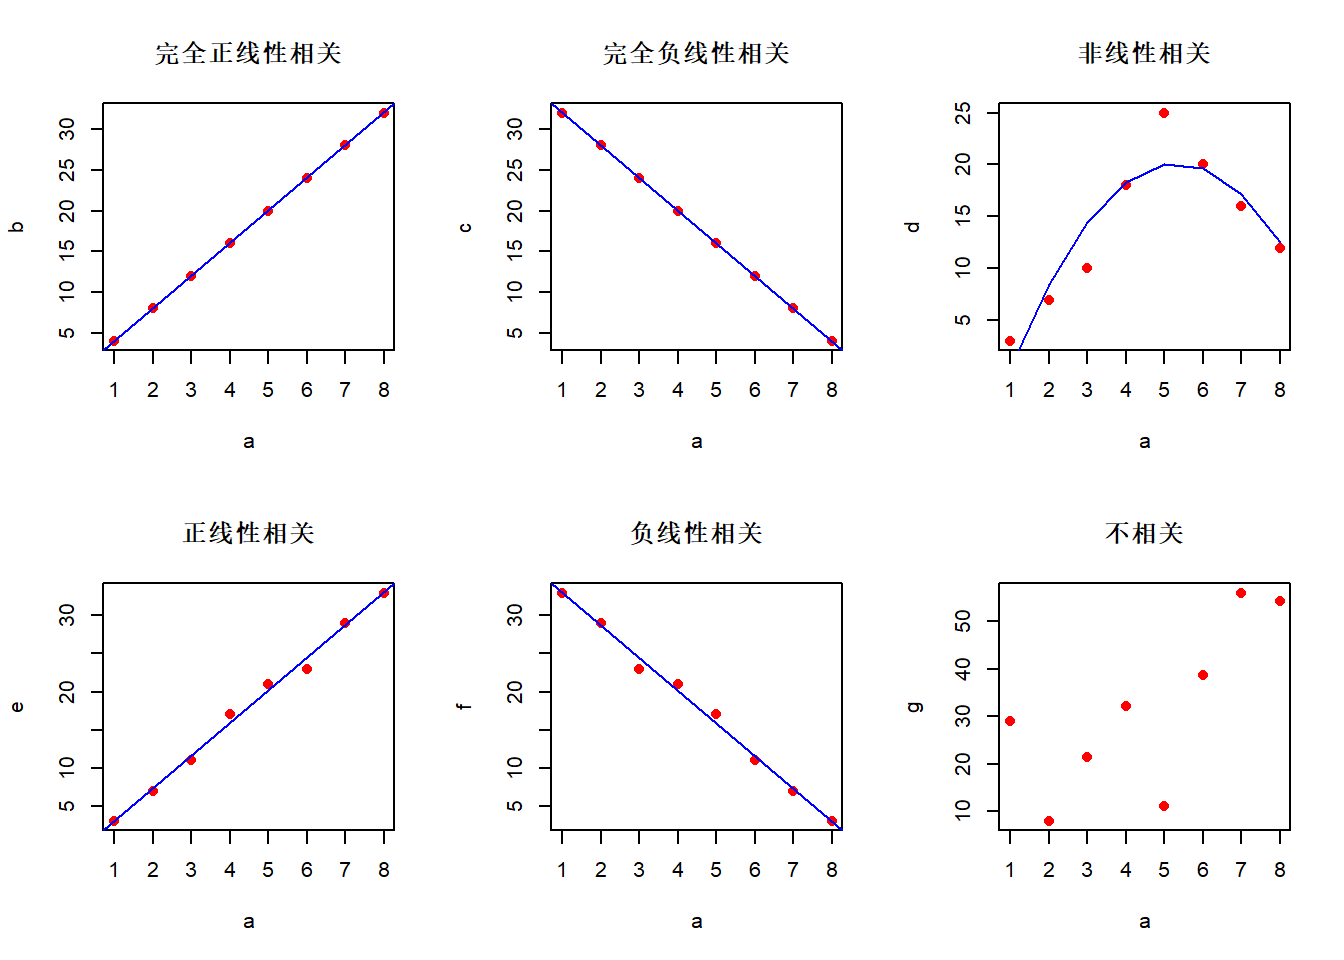
\includegraphics[width=1\linewidth,height=0.35\textheight]{bookdown_files/figure-latex/unnamed-chunk-38-1}

除了如上的图,可以看下面的链接------关于相同统计量不同数据的一篇外文。

\begin{quote}
\begin{itemize}
\tightlist
\item
  \url{https://www.autodeskresearch.com/publications/samestats}
\end{itemize}
\end{quote}

\textbf{相关系数(correlation coefficient)}

\begin{quote}
\begin{itemize}
\tightlist
\item
  对变量之间关系密切程度的度量(只关心密切程度,无关因果关系);
\item
  对两个变量之间线性相关程度的度量称为简单相关系数;
\item
  若相关系数是根据总体全部数据计算的,称为总体相关系数,记为ρ;
\item
  若是根据样本数据计算的,则称为样本相关系数,记为 r。
\end{itemize}
\end{quote}

\textbf{总体相关系数的计算公式}:

\[\rho=\frac{\sigma_{xy}}{\sigma_x\sigma_y}=\frac{E[(X-E(X))(Y-E(Y))]}{\sqrt{E(X-E(X))^2}\sqrt{E(Y-E(Y))^2}}\]

\textbf{相关系数特点}

\begin{quote}
\begin{itemize}
\tightlist
\item
  无量纲(Unitfree);
\item
  \(\rho\)的取值范围是 {[}-1,1{]};
\item
  \(|\rho|\)=1,为完全相关(\(\rho\)=1为完全正相关; \(\rho\)=-1为完全负相关);
\item
  \(\rho\)=0,不存在线性相关关系;
\item
  \(-1\leq \rho<0\),为负相关,\(0<\rho \leq 1\),为正相关;
\item
  \(|\rho|\)越趋于1表示线性关系越密切;\(|\rho|\)越趋于0表示线性关系越不密切;
\item
  若X与Y相互独立,则\(\rho\)=0,但\(\rho\)=0,X与Y不一定相互独立;
\item
  若\(\rho\)= 0,且X与Y服从正态分布,则X与Y相互独立。
\end{itemize}
\end{quote}

\textbf{样本相关系数计算公式}:

\[r=\frac{\sum(x_i-\bar x)(y_i-\bar y)}{\sqrt{\sum(x_i-\bar x)^2\cdot\sum(y_i-\bar y)^2}}\]

或

\[r=\frac{n\sum x_iy_i-\sum x_i\sum y_i}{\sqrt{n\sum x_i^2-(\sum x_i)^2}\cdot\sqrt{n\sum x_i^2-(\sum x_i)^2}}\]

\textbf{样本相关系数特点}

\begin{quote}
\begin{itemize}
\tightlist
\item
  无量纲(Unitfree);
\item
  r的取值范围是 {[}-1,1{]};
\item
  \textbar r\textbar=1,为完全相关(r=1为完全正相关;r=-1为完全负相关);
\item
  r=0,不存在线性相关关系;
\item
  \(-1\leq r<0\)为负相关,\(0<r\leq1\)为正相关;
\item
  \textbar r\textbar 越趋于1表示线性关系越密切;\textbar r\textbar 越趋于0表示线性关系越不密切;
\end{itemize}
\end{quote}

对变量之间关系密切程度的度量,只关心密切程度,无关因果关系。
比如撑伞的人数和降雨量的相关系数非常高。但是我们不能说因为撑伞的人多了,所以降雨量大。

\textbf{r的抽样分布}

r的抽样分布随总体相关系数和样本容量的大小而变化。当样本数据来自服从正态分布的总体时,随着n的增大,r的抽样分布趋于正态分布,尤其是在总体相关系数\(\rho\)很小或接近0时,趋于正态分布的趋势非常明显。而当\(\rho\)远离0时,除非n非常大,否则r的抽样分布呈现一定的偏态。当\(\rho\)为较大的正值时, r呈现左偏分布;当\(\rho\)为较小的负值时, r呈现右偏分布。只有当\(\rho\)接近于0,而样本容量n很大时,才能认为r是接近于正态分布的随机变量。

\textbf{相关系数的显著性检验步骤}

检验两个变量之间是否存在线性相关关系,等价于对回归系数\(\beta_1\)的检验。采用R. A. Fisher提出的t检验。检验的步骤为:

\begin{quote}
(1) 提出假设:\(H_0:\rho=0;H_1:\rho \neq0\)
\end{quote}

\begin{quote}
(2) 计算检验的统计量: \(t=r\sqrt{\frac{n-2}{1-r^2}}\sim t(n-2)\)
\end{quote}

\begin{quote}
(3) 确定显著性水平\(\alpha\),并作出决策。
\end{quote}

\begin{quote}
\begin{itemize}
\tightlist
\item
  若\(|t|>t_{\alpha/2}\),拒绝\(H_0\)。
\item
  若\(|t|<t_{\alpha/2}\),不能拒绝\(H_0\)。
\end{itemize}
\end{quote}

\hypertarget{ux56deux5f52ux5206ux6790ux548cux7b80ux5355ux7ebfux6027ux56deux5f52ux5206ux6790}{%
\section{回归分析和简单线性回归分析}\label{ux56deux5f52ux5206ux6790ux548cux7b80ux5355ux7ebfux6027ux56deux5f52ux5206ux6790}}

\hypertarget{ux56deux5f52ux5206ux6790}{%
\subsection{回归分析}\label{ux56deux5f52ux5206ux6790}}

\textbf{什么是回归分析(Regression)?}

\begin{quote}
从一组样本数据出发,确定变量之间的数学关系式。对这些关系式的可信程度进行各种统计检验,并从影响某一特定变量的诸多变量中找出哪些变量的影响显著, 哪些不显著。利用所求的关系式,根据一个或几个变量的取值来预测或控制另一个特定变量的取值,并给出这种预测或控制的精确程度。
\end{quote}

\textbf{回归分析与相关分析的区别}

\begin{quote}
相关分析中,变量x变量y处于平等的地位;回归分析中,变量y称为因变量,处在被解释的地位,x称为自变量,用于预测因变量的变化;
相关分析中所涉及的变量x和y都是随机变量;回归分析中,因变量y是随机变量,自变量x可以是随机变量,也可以是非随机的确定变量;
相关分析主要是描述两个变量之间线性关系的密切程度;回归分析不仅可以揭示变量x对变量y的影响大小,还可以由回归方程进行预测和控制。
\end{quote}

\textbf{回归模型(regression model)}------回答``变量之间是什么样的关系?''方程中运用1个数值型因变量(响应变量)作为被预测的变量;1个或多个数值型或分类型自变量 (解释变量)作为用于预测的变量。主要用于预测和估计。回归模型的类型包括一元回归模型(线性和非线性)和多元回归模型(线性和非线性)。

接下来先从简单线性回归分析讲起。

\hypertarget{ux7b80ux5355ux7ebfux6027ux56deux5f52ux5206ux6790}{%
\subsection{简单线性回归分析}\label{ux7b80ux5355ux7ebfux6027ux56deux5f52ux5206ux6790}}

\textbf{简单线性回归(Simple Linear Regression)}------涉及一个自变量的回归,因变量y与自变量x之间为线性关系。被预测或被解释的变量称为因变量(dependent variable),用y表示;用来预测或用来解释因变量的一个或多个变量称为自变量(independent variable),用x表示。因变量与自变量之间的关系用一个线性方程来表示。描述因变量y如何依赖于自变量x和误差项ε的方程称为回归模型(Regression Model,定义如前)。

\textbf{(1)简单线性回归模型的表示形式}

\[y=\beta_0+\beta_1 x+\varepsilon\]

y是x的线性函数(部分)加上误差项(residual/random error term)。线性部分反映了由于x的变化而引起的y的变化。误差项ε是随机变量。反映了除x和y之间的线性关系之外的随机因素对y的影响,是不能由x和y之间的线性关系所解释的变异性。\(\beta_0\)和\(\beta_1\)称为模型的参数(interception, slope)。

\textbf{(2)简单线性回归模型的基本假定}

误差项\(\epsilon\)是一个期望值为0的随机变量,即E(\(\epsilon\))=0。对于一个给定的x值,y的期望值为

\[E(y)=\beta_0+\beta_1x\]

对于所有的x值\(\epsilon\)的方差\(\sigma^2\)都相同;误差项\(\epsilon\)是一个服从正态分布的随机变量,且相互独立。即\(\epsilon\sim N(0,\sigma^2)\);独立性意味着对于一个特定的x值,它所对应的\(\epsilon\)与其他x值所对应的\(\epsilon\)不相关;对于一个特定的x值, 它所对应的y值与其他x所对应的y值也不相关。

\textbf{(3)简单线性回归方程(regression equation)}

描述y的平均值或期望值如何依赖于x的方程称为回归方程;简单线性回归方程的形式如下

\[E(y)=\beta_0+\beta_1x\]

方程的图示是一条直线,也称为直线回归方程。\(\beta_0\)是回归直线在y轴上的截距(interception),是当x=0时y的期望值。\(\beta_1\)是直线的斜率(slope),称为回归系数,表示当x每变动一个单位时,y的平均变动值。

\textbf{(4)估计的回归方程(estimated regression equation)}

总体回归参数\(\beta_0\)和\(\beta_1\)是未知的,必须利用样本数据去估计。用样本统计量\(b_0\)和\(b_1\)代替回归方程中的未知参数\(\beta_0\)和\(\beta_1\),就得到了估计的回归方程。简单线性回归中估计的回归方程为

\[\hat y=b_0+b_1x\]

其中:\(b_0\)是估计的回归直线在y轴上的截距,\(b_1\)是直线的斜率,也表示x每变动一个单位时,y的平均变动值,\(\hat y\)表示一个给定的x的值对应的y的估计值。

\textbf{(5)最小二乘估计}

使因变量的观察值与估计值之间的离差平方和达到最小来求得\(b_0\)和\(b_1\)的方法。即

\[argmin \sum_{i=1}^n(y_i-\hat y_i)^2=\sum_{i=1}^n(y_i-b_0-b_ix_i)^2\]

用最小二乘法拟合的直线来代表x与y之间的关系与实际数据的误差平方和比其他任何直线都小。
根据最小二乘法的要求,可得到如下的公式:

\[\begin{cases}b_1=\frac{n\sum_{i=1}^nx_iy_i-(\sum_{i=1}^nx_i)(\sum_{i=1}^ny_i)}{n\sum_{i=1}^nx_i^2-(\sum_{i=1}^nx_i)^2}\\b_0=\bar y-b_1\bar x\end{cases}\]

\textbf{最小二乘估计的性质}

\begin{quote}
\begin{itemize}
\tightlist
\item
  所有残差的和为0。所有残差的平方和最小;
\item
  回归直线经过变量X与Y的均值;
\item
  是\(\beta_0\)和\(\beta_1\)的无偏估计。
\end{itemize}
\end{quote}

在R语言中,简单线性回归的代码如下:

\begin{Shaded}
\begin{Highlighting}[]
\NormalTok{modele<-}\KeywordTok{lm}\NormalTok{(e}\OperatorTok{~}\NormalTok{a)}
\end{Highlighting}
\end{Shaded}

\textbf{(7)回归直线的拟合优度}

\textbf{变差}

因变量 y 的取值是不同的, y 取值的这种波动称为变差。 变差来源于两个方面:

\begin{quote}
\begin{itemize}
\tightlist
\item
  由于自变量 x 的取值不同造成的。
\item
  除 x 以外的其他因素(如x对y的非线性影响、测量误差等)的影响。对一个具体的观测值来说, 变差的大小可以通过该实际观测值与其均值之差\(y-\bar y\)来表示。
\end{itemize}
\end{quote}

\textbf{离差平方和的分解(三个平方和的关系与意义)}

\[\sum_{i=1}^n(y_i-\bar y)^2=\sum_{i=1}^n(\hat y_i-\bar y)^2+\sum_{i=1}^n(y_i-\hat y)^2\]

从左至右分别为SST,SSR,SSE。所以就有SST=SSR+SSE。

\textbf{总平方和(SST)}------反映因变量的 n 个观察值与其均值的总离差;

\textbf{回归平方和(SSR)}------反映自变量 x 的变化对因变量 y 取值变化的影响,或者说,是由于x与y之间的线性关系引起的y的取值变化,也称为可解释的平方和;

\textbf{残差平方和(SSE)}------反映除x以外的其他因素对y取值的影响,也称为不可解释的平方和或剩余平方和。

\textbf{判定系数R²(coefficient of determination)}

回归平方和占总离差平方和的比例。

\[R^2=\frac{SSR}{SST}=\frac{\sum_{i=1}^n(\hat y_i-\bar y)^2}{\sum_{i=1}^n(y_i-\bar y)^2}=1-\frac{\sum_{i=1}^n(y_i-\hat y)^2}{\sum_{i=1}^n(\hat y_i-\bar y)^2}\]

\begin{quote}
\begin{itemize}
\tightlist
\item
  反映回归直线的拟合程度;
\item
  取值范围在{[}0,1{]}之间;
\item
  \(R^2\rightarrow1\),说明回归方程拟合的越好;\(R^2\rightarrow0\),说明回归方程拟合的越差;
\item
  对简单线性回归,判定系数等于相关系数的平方,\(r=(b_1\)的符号)\(sqrt(R^2)\)。
\end{itemize}
\end{quote}

\textbf{估计标准误差(standard error of estimate)}
\textgreater{} * 实际观察值与回归估计值离差平方和的均方根;
\textgreater{} * 反映实际观察值在回归直线周围的分散状况;
\textgreater{} * 对误差项\(\epsilon\)的标准差\(\sigma\)的估计, 是在排除了x对y的线性影响后,y随机波动大小的一个估计量;
\textgreater{} * 反映用估计的回归方程预测y时预测误差的大小。

计算公式为
\[s=\sqrt{\frac{\sum_{i=1}^n(y_i-\hat y_i)^2}{n-2}}=\sqrt{\frac{SSE}{n-2}}=\sqrt{MSE}\]

\textbf{显著性检验}

\begin{quote}
\begin{itemize}
\tightlist
\item
  线性关系的显著性检验:检验自变量与因变量之间的线性关系是否显著,即检验x与y之间是否具有线性关系,或者说,检验自变量x对因变量y的影响是否显著;
\item
  回归系数的显著性检验:检验回归系数是否不等于0;
\item
  在简单线性回归中,线性关系的显著性检验等价于回归系数的显著性检验。
\end{itemize}
\end{quote}

\textbf{线性关系的检验}

将回归均方(MSR)同残差均方(MSE)加以比较, 应用F检验来分析二者之间的差别是否显著。

\begin{quote}
\begin{itemize}
\tightlist
\item
  \textbf{回归均方}:回归平方和SSR除以相应的自由度(自变量的个数p);
\item
  \textbf{残差均方}:残差平方和SSE除以相应的自由度(n-p-1)。
\item
  提出假设:\(H_0:\beta_1=0\)线性关系不显著;
\item
  计算检验统计量F:\(F=\frac{SSR/1}{SSE/(n-2)}=\frac{MSR}{MSE}\sim F(1,n-2)\)
\item
  确定显著性水平\(\alpha\),并根据分子自由度1和分母自由度n-2找出临界值\(F_\alpha\)。
\item
  作出决策:若\(F>F_\alpha\),拒绝\(H_0\); 若\(F<F_\alpha\),不拒绝\(H_0\)。
\end{itemize}
\end{quote}

\textbf{回归系数的检验(检验步骤)}

\begin{quote}
\begin{itemize}
\tightlist
\item
  提出假设:\(H_0:\beta_1=0\)(没有线性关系),\(H_1:\beta_1\neq 0\)(有线性关系)
\item
  计算检验的统计量:\(t=\frac{b_1}{s_{b_1}}\sim t(n-2)\)
\item
  确定显著性水平\(\alpha\),并进行决策:\(|t|> t_{\alpha/2}\),拒绝\(H_0\);\(|t|< t_{\alpha/2}\),不拒绝\(H_0\)
\end{itemize}
\end{quote}

\textbf{显著性检验的几点注意}

显著性关系的结论不意味着因果关系。显著性关系的结论也不能推出线性关系的结论,仅能说在x的样本观测之范围内,x和y是相关的,而且一个线性关系只揭示了y的变异的主要部分。当样本容量很大时,对于小的b1值也能得到统计上是显著的结果。

\hypertarget{ux5229ux7528ux56deux5f52ux65b9ux7a0bux8fdbux884cux4f30ux8ba1ux548cux9884ux6d4b}{%
\section{利用回归方程进行估计和预测}\label{ux5229ux7528ux56deux5f52ux65b9ux7a0bux8fdbux884cux4f30ux8ba1ux548cux9884ux6d4b}}

根据自变量x的取值估计或预测因变量y的取值。

\textbf{估计或预测的类型}

(1)点估计:y的平均值的点估计,y的个别值的点估计;

(2)区间估计:y的平均值的置信区间估计,y的个别值的预测区间估计。

\textbf{(1)点估计}

对于自变量x的一个给定值\(x_0\),根据回归方程得到因变量y的一个估计值\(\hat y_0\)。点估计值有\textbf{y的平均值的点估计}和\textbf{y的个别值的点估计}。在点估计条件下,平均值的点估计和个别值的的点估计是一样的,但在区间估计中则不同。

\begin{quote}
\textbf{y的平均值的点估计}:利用估计的回归方程, 对于自变量x的一个给定值\(x_0\),求出因变量y的平均值的一个估计值\(E(y_0)\),就是平均值的点估计。
\end{quote}

\begin{quote}
\textbf{y的个别值的点估计}:利用估计的回归方程,对于自变量x的一个给定值\(x_0\),求出因变量y的一个个别值的估计值\(\hat y_0\),就是个别值的点估计。
\end{quote}

\textbf{(2)区间估计}

点估计不能给出估计的精度, 点估计值与实际值之间是有误差的,因此需要进行区间估计。对于自变量x的一个给定值\(x_0\),根据回归方程得到因变量y的一个估计区间。区间估计有两种类型:\textbf{置信区间估计(confidence interval estimate)}和\textbf{预测区间估计(prediction interval estimate)}。

\textbf{置信区间估计}

利用估计的回归方程,对于自变量x的一个给定值\(x_0\),求出因变量y的平均值的估计区间,这一估计区间称为置信区间(confidence interval)。\(E(y_0)\)在\(1-\alpha\)置信水平下的置信区间为:

\[\hat y_0\pm t_{\alpha/2}(n-2)s\sqrt{\frac{1}{n}+\frac{(x_0-\bar x)^2}{\sum_{i=1}^n(x_i-\bar x)^2}}\]

式中s为估计标准误差。x=均值时能得到y的平均值的最精确估计。

\textbf{预测区间估计}

利用估计的回归方程,对于自变量x的一个给定值\(x_0\),求出因变量y的一个个别值的估计区间,这一区间称为预测区间(prediction interval)。\(E(y_0)\)在\(1-\alpha\)置信水平下的预测区间为:

\[\hat y_0\pm t_{\alpha/2}(n-2)s\sqrt{1+\frac{1}{n}+\frac{(x_0-\bar x)^2}{\sum_{i=1}^n(x_i-\bar x)^2}}\]

\textbf{影响区间宽度的因素}
\textgreater{} * 置信水平(\(1-\alpha\))------区间宽度随置信水平的增大而增大;
\textgreater{} * 数据的离散程度s------区间宽度随离散程度的增大而增大;
\textgreater{} * 样本容量------区间宽度随样本容量的增大而减小;
\textgreater{} * 用于预测的\(x_p\)与\(\bar x\)的差异程度,区间宽度随\(x_p\)与\(\bar x\)的差异程度的增大而增大。

其实在R语言里主要用predict.lm函数来进行区间估计。代码样例如下:

\begin{Shaded}
\begin{Highlighting}[]
\NormalTok{con <-}\StringTok{ }\KeywordTok{predict.lm}\NormalTok{(modele, h, }\DataTypeTok{interval=}\StringTok{"confidence"}\NormalTok{,}\DataTypeTok{level=}\FloatTok{0.95}\NormalTok{)}
\end{Highlighting}
\end{Shaded}

其中interval控制是置信区间(参数填confidence)、预测区间(参数填prediction)或者是不做区间估计,level是置信水平,接着用R绘制一个简单的回归和置信区间的图,这里先给出如何绘制置信区间band的代码,完整代码还是老规矩,在这一部分笔记写完后给出。

\begin{Shaded}
\begin{Highlighting}[]
\KeywordTok{polygon}\NormalTok{(}\KeywordTok{c}\NormalTok{(h[,}\DecValTok{1}\NormalTok{], }\KeywordTok{rev}\NormalTok{(h[,}\DecValTok{1}\NormalTok{])), }\KeywordTok{c}\NormalTok{(con[,}\DecValTok{3}\NormalTok{], }\KeywordTok{rev}\NormalTok{(con[,}\DecValTok{2}\NormalTok{])), }\DataTypeTok{border=}\StringTok{"red"}\NormalTok{,}\DataTypeTok{lwd=}\DecValTok{1}\NormalTok{,}\DataTypeTok{lty =} \KeywordTok{c}\NormalTok{(}\StringTok{"dashed"}\NormalTok{, }\StringTok{"solid"}\NormalTok{))}
\end{Highlighting}
\end{Shaded}

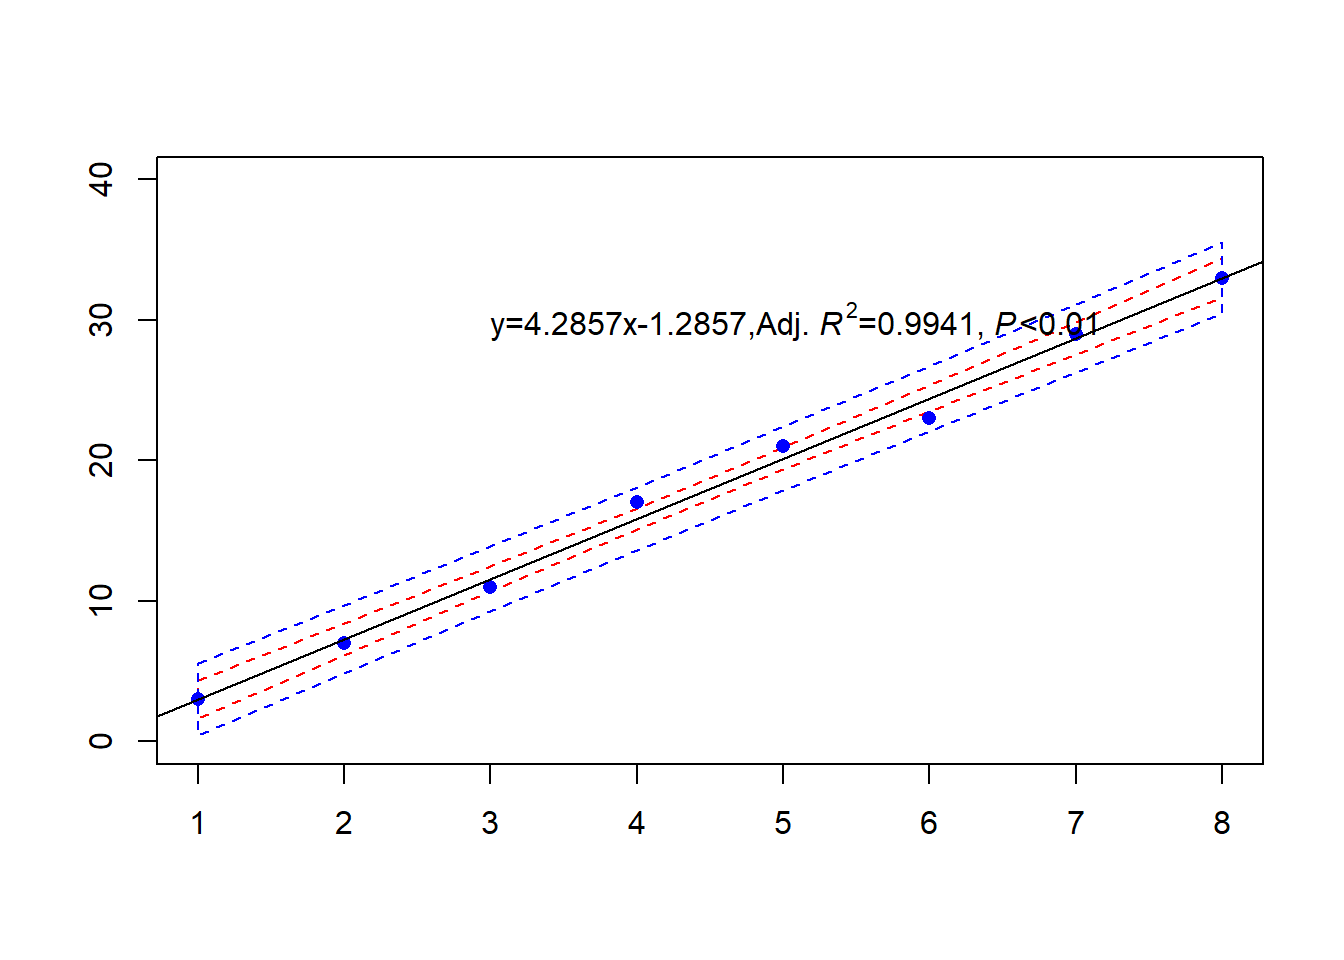
\includegraphics[width=1\linewidth,height=0.4\textheight]{bookdown_files/figure-latex/unnamed-chunk-42-1}

\hypertarget{ux6b8bux5deeux5206ux6790}{%
\section{残差分析}\label{ux6b8bux5deeux5206ux6790}}

\textbf{残差(residual)}------因变量的观测值与根据估计的回归方程求出的预测值之差,用e表示。

\[e_i=y_i-\hat y_i\]

反映了用估计的回归方程去预测而引起的误差。

\textbf{残差检验的目的}

\begin{quote}
\begin{itemize}
\tightlist
\item
  检验线性的假设是否成立;
\item
  确定有关误差项ε的假定是否成立(正态分布;方差为常数;独立性)。
\item
  检测有影响的观测值。
\end{itemize}
\end{quote}

\textbf{残差图(residual plot)}

\begin{quote}
\begin{itemize}
\tightlist
\item
  表示残差的图形(关于x的残差图,关于y的残差图,标准化残差图)。
\item
  用直方图或正态概率图检验正态性。
\end{itemize}
\end{quote}

\textbf{标准化残差(standardized residual)}

\begin{quote}
\begin{itemize}
\tightlist
\item
  残差除以它的标准差后得到的数值。 计算公式为\(z_{e_i}=\frac{e_i}{s_{e_i}}=\frac{y_i-\hat y_i}{s_{e_i}}\)
\item
  \(e_i\)是第i个残差的标准差, 其计算公式为\(s_{e_i}=s_y\sqrt{1-h_i}=s_y\sqrt{1-(\frac{1}{n}+\frac{(x_i-\bar x)^2}{\sum(x_i-\bar x)^2})}\)
\end{itemize}
\end{quote}

\textbf{标准化残差图}

用以直观地判断误差项服从正态分布这一假定是否成立。

\begin{quote}
\begin{itemize}
\tightlist
\item
  若假定成立, 标准化残差的分布也应服从正态分布。
\item
  在标准化残差图中, 大约有95\%的标准化残差在-2到+2之间。
\end{itemize}
\end{quote}

\textbf{变换}

数据变换的问题在前面第七章拟合优度检验提过,那么什么时候做变换?如果从散点图观察发现残差是自变量的函数,通过变换可能可以解决问题。做什么变换?观察残差与因变量观测值的均值的关系:

\begin{quote}
\begin{itemize}
\tightlist
\item
  如果残差的标准差与因变量观测值的均值有线性关系,用log变换;
\item
  如果残差的方差与因变量观测值的均值有线性关系,用square root变换;
\item
  如果残差的标准差与因变量观测值的均值的平方有线性关系,用inverse变换;
\item
  如果残差的标准差与因变量观测值的均值的幂有线性关系,用power变换。
\end{itemize}
\end{quote}

\textbf{序列相关(自相关)}

当数据是按时间顺序采集的,有可能引起误差项之间的相关(Serial correlation,autocorrelation)。这里介绍一个相关的杜宾-瓦特森(Durbin-Watson)检验统计量:

\[d=\frac{\sum_{t=2}^n(e_t-e_{t-1})^2}{\sum_{t=1}^ne_t^2}\]

是否遗漏了重要的对因变量有时序影响的自变量,有时可通过引入度量观测次数的自变量解决该问题。这部分属于时间序列分析的范畴,这里就不进一步阐述了。

在R语言中,线性回归方程残差图绘制非常简单。模型拟合过程会自动给出四个残差可视化相关的图。绘制方法如下:

\begin{Shaded}
\begin{Highlighting}[]
\KeywordTok{layout}\NormalTok{(}\KeywordTok{matrix}\NormalTok{(}\KeywordTok{c}\NormalTok{(}\DecValTok{1}\NormalTok{,}\DecValTok{2}\NormalTok{,}\DecValTok{3}\NormalTok{,}\DecValTok{4}\NormalTok{),}\DataTypeTok{nrow=}\DecValTok{2}\NormalTok{,}\DataTypeTok{byrow=}\NormalTok{T))}
\KeywordTok{plot}\NormalTok{(modele)}
\end{Highlighting}
\end{Shaded}

结果如图。

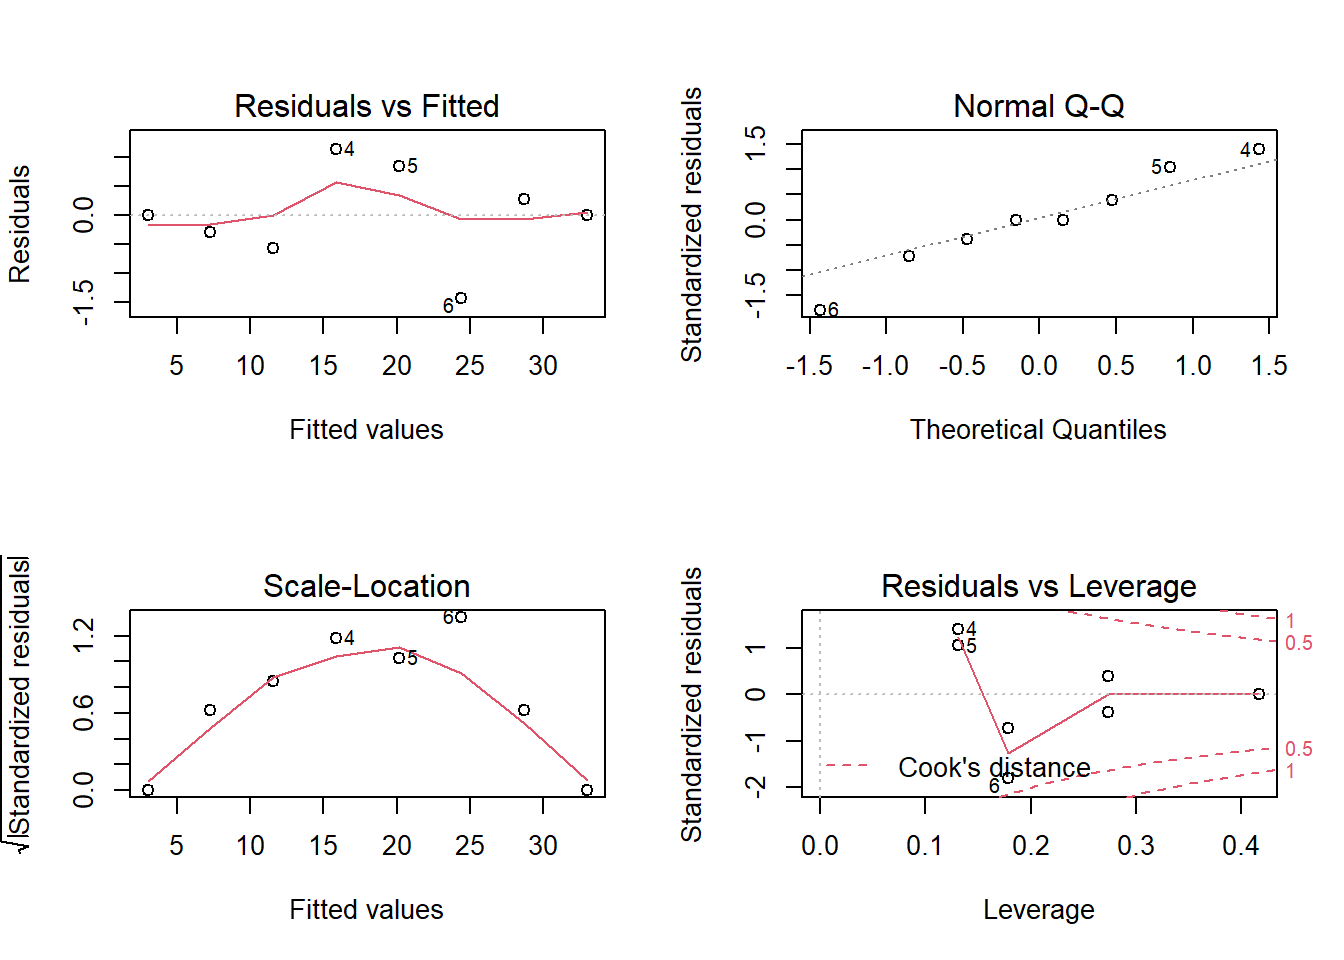
\includegraphics[width=1\linewidth,height=0.4\textheight]{bookdown_files/figure-latex/unnamed-chunk-44-1}

\textbf{异常值(outlier)与识别}

如果某一个点与其他点所呈现的趋势不相吻合,这个点就有可能是异常点。

\begin{quote}
\begin{itemize}
\tightlist
\item
  如果异常值是一个错误的数据, 比如记录错误造成的, 应该修正该数据, 以便改善回归的效果;
\item
  如果是由于模型的假定不合理, 使得标准化残差偏大, 应该考虑采用其他形式的模型,比如非线性模型;
\item
  如果完全是由于随机因素而造成的异常值, 则应该保留该数据。
\end{itemize}
\end{quote}

在处理异常值时, 若一个异常值是一个有效的观测值, 不应轻易地将其从数据集中予以剔除。

\begin{quote}
\begin{itemize}
\tightlist
\item
  异常值也可以通过标准化残差来识别;
\item
  如果某一个观测值所对应的标准化残差较大, 就可以识别为异常值;
\item
  一般情况下,当一个观测值所对应的标准化残差小于-2或大于+2时,就可以将其视为异常值。
\end{itemize}
\end{quote}

\textbf{有影响的观测值}

如果某一个或某一些观测值对回归的结果有强烈的影响,那么该观测值或这些观测值就是有影响的观测值。一个有影响的观测值可能是:一个异常值, 即有一个值远远偏离了散点图中的趋势线;对应一个远离自变量平均值的观测值;或者是这二者组合而形成的观测值。如果有影响的观测值是一个错误的数据,比如记录错误造成的, 应该修正该数据,以便改善回归的效果。如果有影响的观测值是一个有效的数据则应该保留它, 可以帮助我们分析模型的假定是否合理。

\textbf{杠杆率点(leverage point)}

如果自变量存在一个极端值, 该观测值则称为高杠杆率点(high leverage point),在简单回归中,第i个观测值的杠杆率用\(h_i\)表示,其计算公式为:

\[h_i=\frac{1}{n}+\frac{(x_i-\bar x)^2}{\sum(x_i-\bar x)^2}\]

如果一个观测值的杠杆率\(h_i>n/6\),就可以将该观测值识别为有高杠杆率的点;一个有高杠杆率的观测值未必是一个有影响的观测值, 它可能对回归直线的斜率没有什么影响。

\hypertarget{ux591aux5143ux7ebfux6027ux56deux5f52multiple-regression-model}{%
\section{多元线性回归(multiple regression model)}\label{ux591aux5143ux7ebfux6027ux56deux5f52multiple-regression-model}}

\textbf{多元线性回归(multiple regression model)}

\begin{quote}
\begin{itemize}
\tightlist
\item
  一个因变量与两个及两个以上自变量的回归。
\item
  描述因变量y如何依赖于自变量\(x_1,x_2,\cdots,x_p\)和误差项\(\varepsilon\)的方程,称为多元回归模型。
\item
  涉及p个自变量的多元回归模型可表示为
\end{itemize}
\end{quote}

\[y=\beta_0+\beta_1x_1+\beta_2x_2+\cdots+\beta_px_p+\varepsilon\]

\begin{quote}
\begin{itemize}
\tightlist
\item
  \(\beta_0,\beta_1,\beta_2,\cdots,\beta_p\)是参数。
\item
  \(\varepsilon\)是被称为误差项的随机变量。
\item
  y是\(x_1,x_2,\cdots,x_p\)的线性函数加上误差项\(\varepsilon\)。
\item
  \(\varepsilon\)包含在y里面但不能被p个自变量的线性关系所解释的变异性。
\end{itemize}
\end{quote}

\textbf{多元回归模型的基本假定}

\begin{quote}
\begin{itemize}
\tightlist
\item
  误差项\(\epsilon\)是一个期望值为0的随机变量, 即\(E(\epsilon)=0\)。
\item
  对于自变量\(x_1,x_2,\cdots,x_p\)的所有值,\(\epsilon\)的方差\(\sigma^2\)都相同。
\item
  误差项\(\epsilon\)是一个服从正态分布的随机变量,即\(\varepsilon\sim N(0,\sigma^2)\),且相互独立。
\end{itemize}
\end{quote}

\textbf{多元回归方程(multiple regression equation)}

描述因变量y的平均值或期望值如何依赖于自变量\(x_1,x_2,\cdots,x_p\)的方程。多元线性回归方程的形式为:

\[E(y)=\beta_0+\beta_1x_1+\beta_2x_2+\cdots+\beta_px_p+\varepsilon\]

\begin{quote}
\begin{itemize}
\tightlist
\item
  \(\beta_1,\beta_2,\cdots,\beta_p\)称为偏回归系数。
\item
  \(\beta_i\)表示假定其他变量不变,当\(x_i\)每变动一个单位时,y的平均变动值。
\end{itemize}
\end{quote}

二元回归方程的几何表达------回归面。

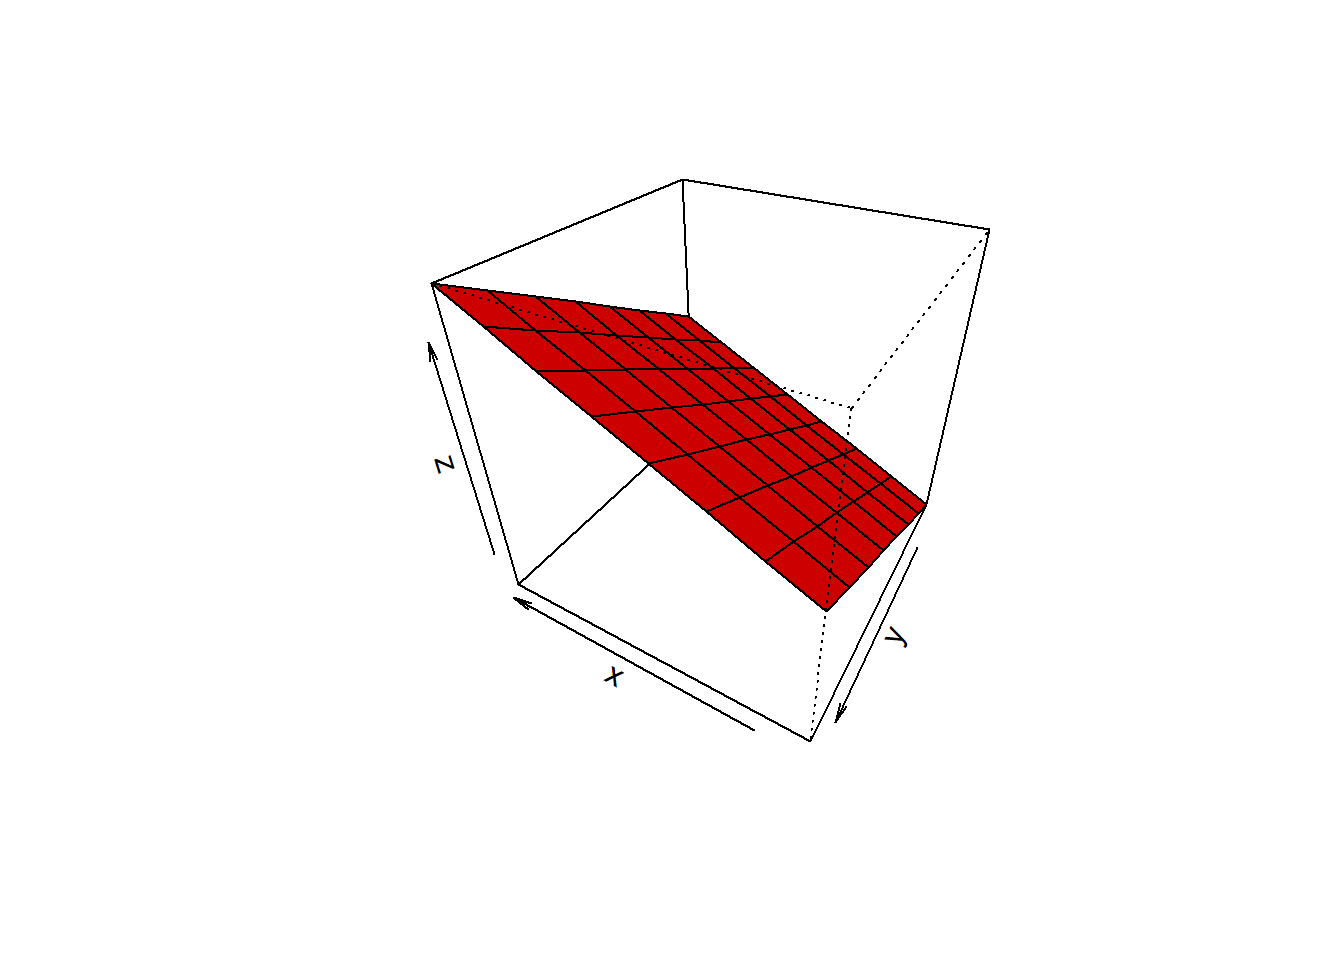
\includegraphics[width=1\linewidth,height=0.4\textheight]{bookdown_files/figure-latex/unnamed-chunk-45-1}

\textbf{估计的多元回归的方程(estimated multiple regression equation)}

用样本统计量\(b_0,b_1,b_2,\cdots,b_p\)估计回归方程中的参数\(\beta_0,\beta_1,\beta_2,\cdots,\beta_p\)时得到的方程。一般形式为

\[\hat y=b_0+b_1x_1+b_2x_2+\cdots+b_px_p\]

\textbf{参数的最小二乘法}

使因变量的观察值与估计值之间的离差平方和达到最小来求得\(b_0,b_1,b_2,\cdots,b_p\),即:\(argmin Q(b_0,b_1,b_2,\cdots,b_p)=\sum_{i=1}^n(y_i-\hat y_i)^2=\sum_{i=1}^ne_i^2\)

求解各回归参数的标准方程如下:

\[\begin{cases}\left. \frac{\partial Q}{\partial \beta_0} \right| _{\beta_0=b_0}=0\\\left. \frac{\partial Q}{\partial \beta_i} \right| _{\beta_i=b_i}=0(i=1,2,\cdots,p)\end{cases}\]

\textbf{多重判定系数(multiple coefficient of determination)}

回归平方和占总平方和的比例,计算公式为

\[R^2=\frac{\sum_{i=1}^n(\hat y_i-\bar y)^2}{\sum_{i=1}^n(y_i-\bar y)^2}=\frac{SSR}{SST}=1-\frac{SSE}{SST}\]

因变量取值的变差中, 能被估计的多元回归方程所解释的比例。

\textbf{修正多重判定系数(adjusted multiple coefficient of determination)}

用样本容量n和自变量的个数p去修正\(R^2\)得到。计算公式为

\[R_a^2=1-(1-R^2)\times\frac{n-1}{n-p-1}\]

避免增加自变量而高估\(R^2\),意义与\(R^2\)类似,数值小于\(R^2\)。

\textbf{估计标准误差s}

对误差项\(\epsilon\)的标准差\(\sigma\)的一个估计值。衡量多元回归方程的拟合优度。计算公式为

\[s=\sqrt{\frac{\sum_{i=1}^n(y_i-\hat y_i)^2}{n-p-1}}=\sqrt{\frac{SSE}{n-p-1}}=\sqrt{MSE}\]

\textbf{线性关系检验}

检验因变量与所有自变量之间的线性关系是否显著,也被称为总体的显著性检验。检验方法是将回归均方和(MSR)同离差均方和(MSE)加以比较,应用F检验来分析二者之间的差别是否显著。

\begin{quote}
\begin{itemize}
\tightlist
\item
  如果是显著的, 因变量与自变量之间存在线性关系;
\item
  如果不显著, 因变量与自变量之间不存在线性关系。
\end{itemize}
\end{quote}

(1)提出假设:\(H_0:\beta_1=\beta_2=\cdots=\beta_p=0\) 线性关系不显著;\(H_1:\beta_1,\beta_2,\cdots,\beta_p\) 至少有一个不等于0。

(2)计算检验统计量F:

\[F=\frac{SSR/p}{SSE/(n--p-1)}=\frac{MSR}{MSE}\sim F(p,n-p-1)\]

(3)确定显著性水平\(\alpha\),并根据分子自由度p和分母自由度n-p-1找出临界值\(F_\alpha\)。

(4)作出决策:若\(F>F_\alpha\),拒绝\(H_0\)。

\textbf{回归系数的检验(检验步骤)}

\begin{quote}
\begin{itemize}
\tightlist
\item
  线性关系检验通过后,对各个回归系数进行检验。
\item
  对每一个自变量单独应用 t 检验统计量进行检验。
\end{itemize}
\end{quote}

(1)提出假设:\(H_0:\beta_i=0)\)(自变量\(x_i\)与因变量y没有线性关系,\(H_1:\beta_i\neq 0\)(自变量\(x_i\)与因变量y有线性关系)

(2)计算检验的统计量

\[t=\frac{b_i}{s_{b_i}}\sim t(n-p-1),s_{b_i}=\frac{s}{\sqrt{\sum(x_i-\bar x)^2}}\]

(3)确定显著性水平\(\alpha\),并进行决策:\(|t|> t_{\alpha/2}\),拒绝\(H_0\);\(|t|< t_{\alpha/2}\),不拒绝\(H_0\)

\textbf{回归系数的推断(置信区间)}

回归系数在(\(1-\alpha\))\%置信水平下的置信区间为

\[b_i\pm t_{\alpha/2}(n-p-1)s_{b_i}\]

回归系数的抽样标准差

\[s_{b_i}=\frac{s}{\sqrt{\sum(x_i-\bar x)^2}}\]
\#\# 多重共线性(multicollinearity)
回归模型中两个或两个以上的自变量彼此相关。多重共线性带来的问题有:可能会使回归的结果造成混乱, 甚至会把分析引入歧途;可能对参数估计值的正负号产生影响, 特别是各回归系数的正负号有可能同我们预期的正负号相反。

\textbf{多重共线性的识别}

\begin{quote}
\begin{itemize}
\tightlist
\item
  检测多重共线性的最简单的一种办法是计算模型中各对自变量之间的相关系数, 并对各相关系数进行显著性检验;若有一个或多个相关系数显著, 就表示模型中所用的自变量之间相关,存在着多重共线性。
\item
  如果出现下列情况,暗示存在多重共线性:模型中各对自变量之间显著相关。当模型的线性关系检验(F检验)显著时,几乎所有回归系数的t检验却不显著。回归系数的正负号与预期的相反。
\end{itemize}
\end{quote}

\textbf{检测多重共线性(Variance Inflationary Factor)}

VIF (variance inflation factor) 用以测量如果自变量相关对估计的回归系数的变异程度的影响。\(VIF_j\)的定义:\(VIF_j=\frac{1}{1-R_j^2}\)。\(R_2^j\)是第j个自变量对其它自变量进行回归的判定系数。VIF=1表示所对应自变量与其它自变量无线性关系。VIF值越大,多重共线性越严重。如果\(VIF_j>5\),\(x_j\)与其它自变量高度相关。

\textbf{多重共线性(问题的处理)}

将一个或多个相关的自变量从模型中剔除,使保留的自变量尽可能不相关。如果要在模型中保留所有的自变量,则应避免根据t统计量对单个参数进行检验,对因变量值的推断(估计或预测)的限定在自变量样本值的范围内。

\hypertarget{ux5b9aux6027ux81eaux53d8ux91cfux7684ux56deux5f52}{%
\section{定性自变量的回归}\label{ux5b9aux6027ux81eaux53d8ux91cfux7684ux56deux5f52}}

\textbf{虚拟变量(dummy variable)}

定性自变量------------只有两个水平的定性自变量或有两个以上水平的定性自变量。虚拟变量------用数字代码表示的定性自变量。虚拟变量的取值为0,1。

\textbf{虚拟变量的个数}

当定性自变量只有两个水平时,可在回归中引入一个虚拟变量。一般而言,如果定性自变量有k个水平,需要在回归中模型中引进k-1个虚拟变量。当定性自变量只有两个水平并引进虚拟变量时,回归方程可写\(E(y)=\beta_0+\beta_1x\)。当指定虚拟变量0,1时,\(\beta_0\)总是代表与虚拟变量值0所对应的那个分类变量水平的平均值;\(\beta_1\)总是代表与虚拟变量值1所对应的那个分类变量水平的平均响应与虚拟变量值0所对应的那个分类变量水平的平均值的差值,即平均值的差值=\((\beta_0+\beta_1)-\beta_0=\beta_1\)。当定性自变量超过两个水平(假定三个水平)并引进虚拟变量时,回归方程可写\(E(y)=\beta_0+ \beta_1x_1+\beta_2x_2\)。
方差分析同样可以通过引入虚拟变量做回归分析。

\hypertarget{ux975eux7ebfux6027ux56deux5f52}{%
\section{非线性回归}\label{ux975eux7ebfux6027ux56deux5f52}}

\textbf{(1)二阶回归模型(Quadratic Regression Model)}------当散点图如下所示,可考虑二次回归模型。

\[y_i=\beta_0+\beta_1x_i+\beta_2x_i^2+\varepsilon\]

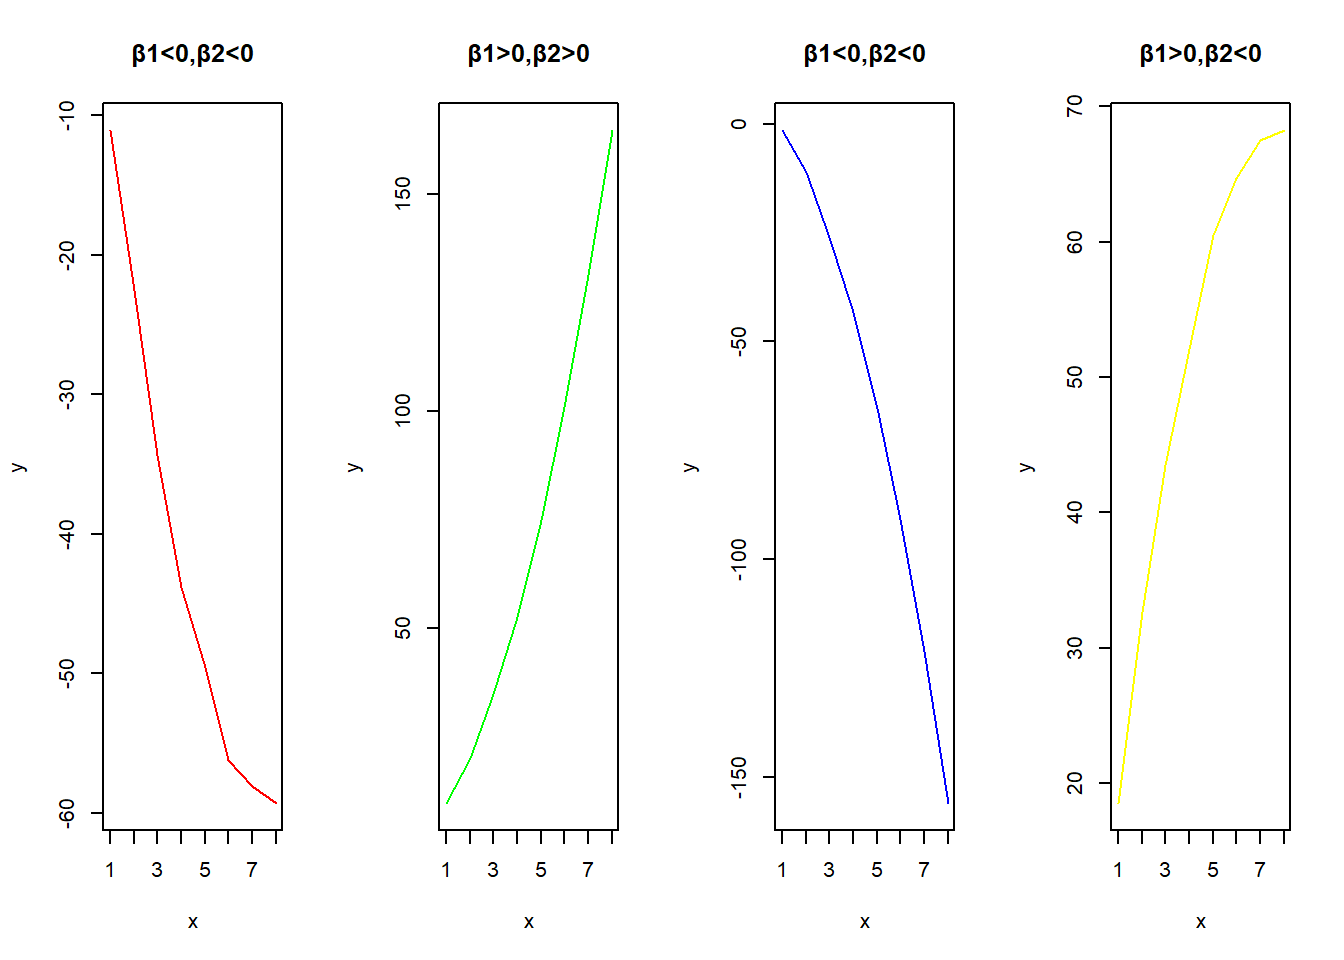
\includegraphics[width=1\linewidth,height=0.4\textheight]{bookdown_files/figure-latex/unnamed-chunk-46-1}

\textbf{二阶回归模型的显著性检验}

\begin{quote}
\begin{itemize}
\tightlist
\item
  总体显著性检验,\(F test statistic=\frac{MSR}{MSE}\)
\item
  二阶检验:比较二阶模型,\(y=\beta_0+\beta_1x_1+\beta_2x^2+\varepsilon\);线性模型,\(y=\beta_0+\beta_1x_1+\varepsilon\)。假设:\(H_0:\beta_2=0\)(没有二阶项),\(H_1:\beta_2\neq 0\)(需要二阶项)。
\end{itemize}
\end{quote}

\textbf{(2)交互作用}

交互作用------两个自变量共同作用对因变量产生的潜在影响。
\textgreater{} * 假设:\(y=\beta_0+\beta_1x_1+\beta_2x_2+\beta_3x_1x_2+\varepsilon\)没有交互项,\(x_1\)对y的影响用\(\beta_1\)测量;有交互项,\(x_1\)对y的影响用\(\beta_1+\beta_3x_2\)测量。影响随\(x_2\)的改变而改变。

\textbf{交互作用显著性检验}

\begin{quote}
\begin{itemize}
\tightlist
\item
  交互作用模型:\(y=\beta_0+\beta_1x_1+\beta_2x_2+\beta_3x_1x_2+\varepsilon\)
\item
  假设:\(H_0:\beta_3=0\)(\(x_1\)和\(x_2\)无交互作用),\(H_1:\beta_3\neq 0\)(\(x_1\)和\(x_2\)有交互作用)
\end{itemize}
\end{quote}

\textbf{(3)其他非线性回归}

因变量y与x之间不是线性关系,可通过变量代换转换成线性关系,用最小二乘法求出参数的估计值。但是并非所有的非线性模型都可以化为线性模型。

\begin{itemize}
\tightlist
\item
  双曲线
\end{itemize}

基本形式:

\[y=\frac{x}{\alpha x+\beta}\]
线性化方法:令\(y'=\frac{1}{y},x'=\frac{1}{x}\),则有\(y'=\alpha+\beta x'\)

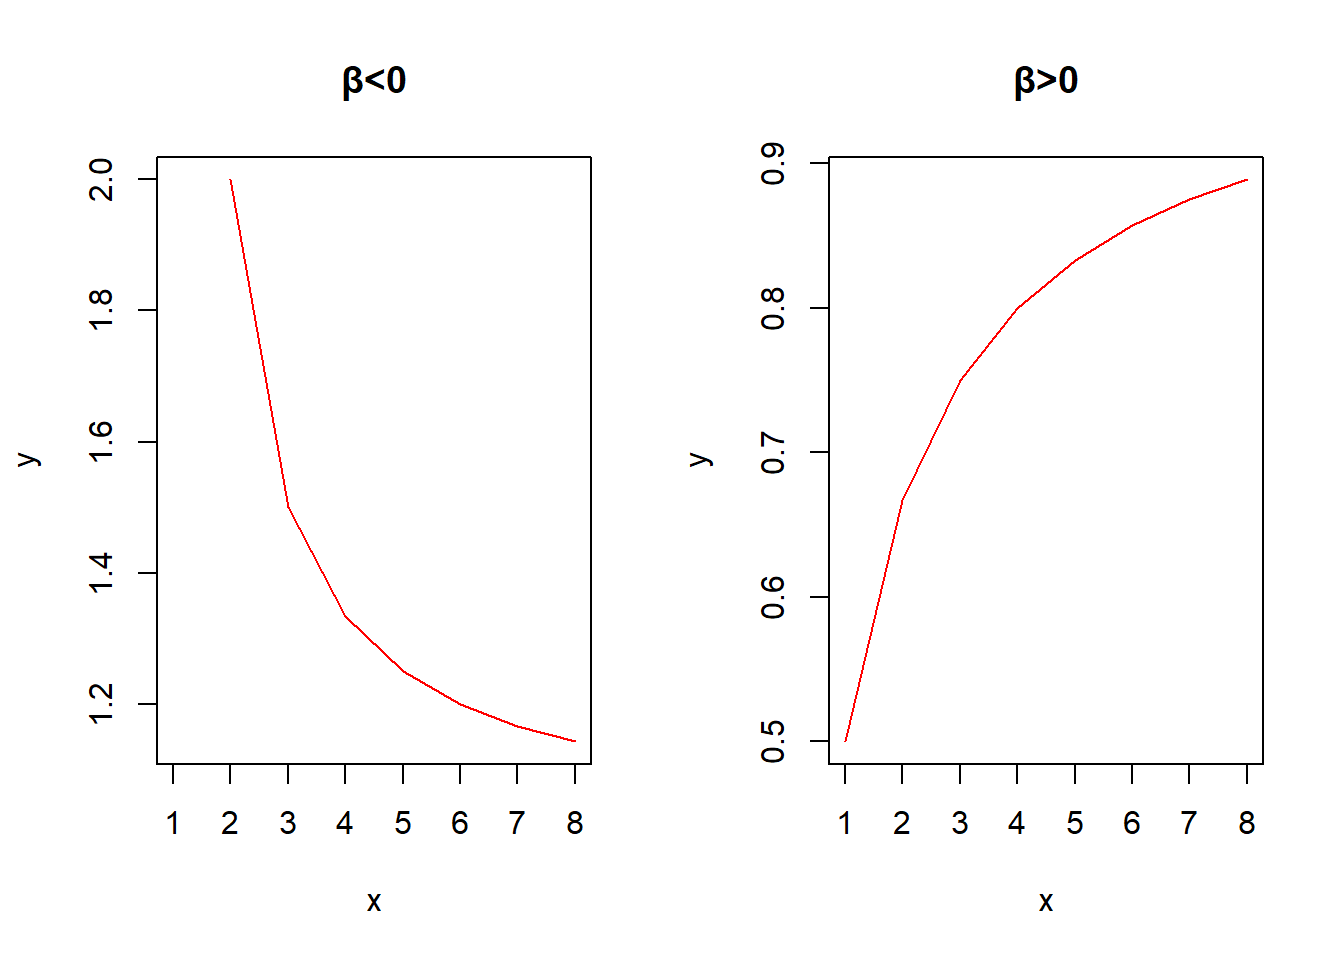
\includegraphics[width=1\linewidth,height=0.4\textheight]{bookdown_files/figure-latex/unnamed-chunk-47-1}

\begin{itemize}
\tightlist
\item
  幂函数曲线
\end{itemize}

基本形式:

\[y=\alpha x^\beta\]

线性化方法:两端取对数得\(lgy=lg\alpha+\beta lgx,y'=lgy,x'=lgx\),则有\(y'=lg\alpha+\beta x'\)

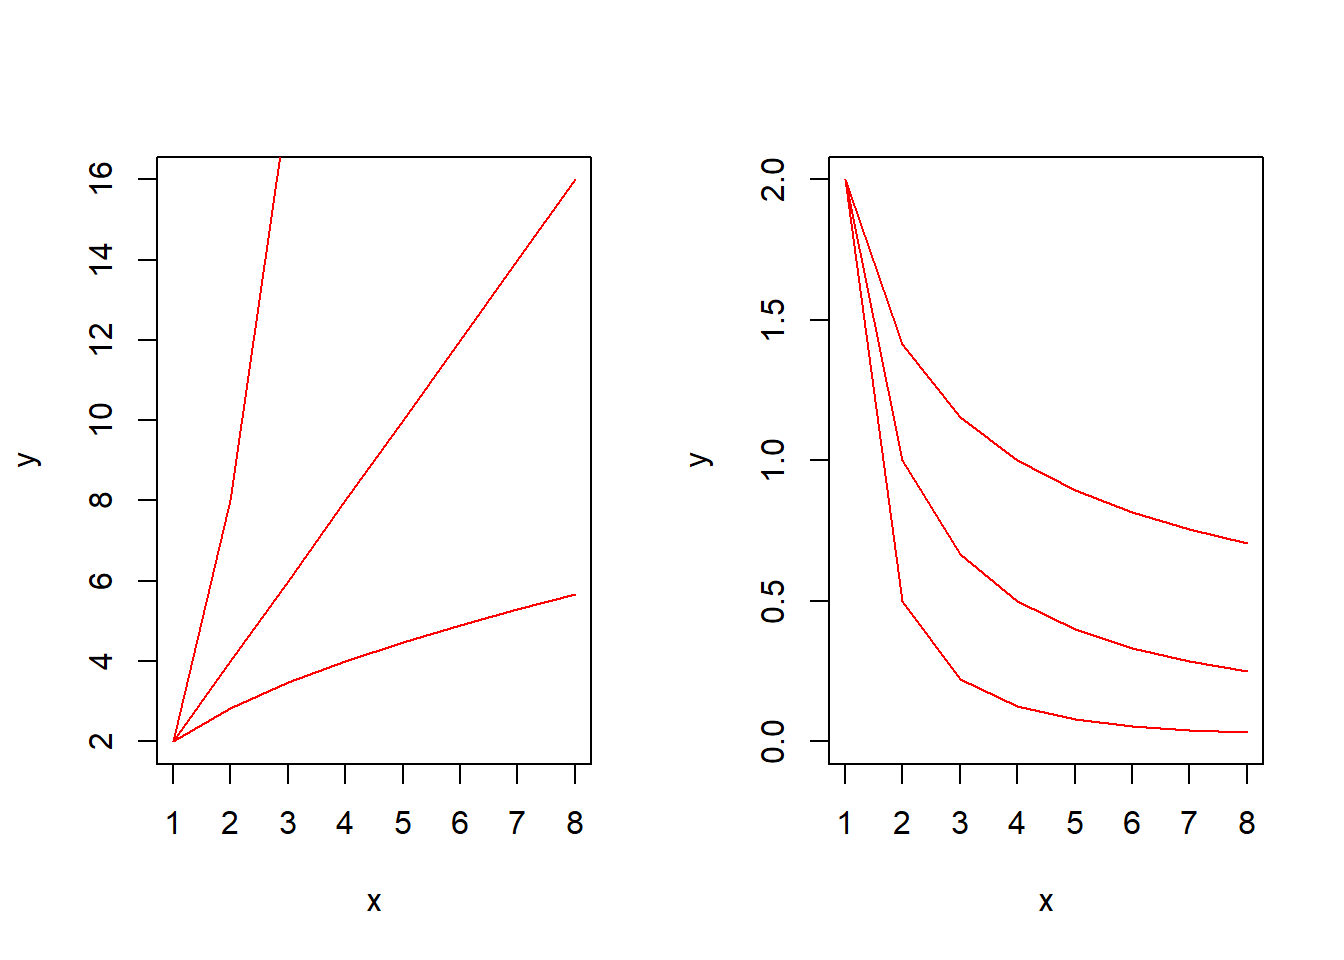
\includegraphics[width=1\linewidth,height=0.4\textheight]{bookdown_files/figure-latex/unnamed-chunk-48-1}

\begin{itemize}
\tightlist
\item
  对数曲线
\end{itemize}

基本形式:

\[y=\alpha+\beta lnx\]

线性化方法:\(x'=lnx\),则有\(y'=\alpha+\beta x'\)

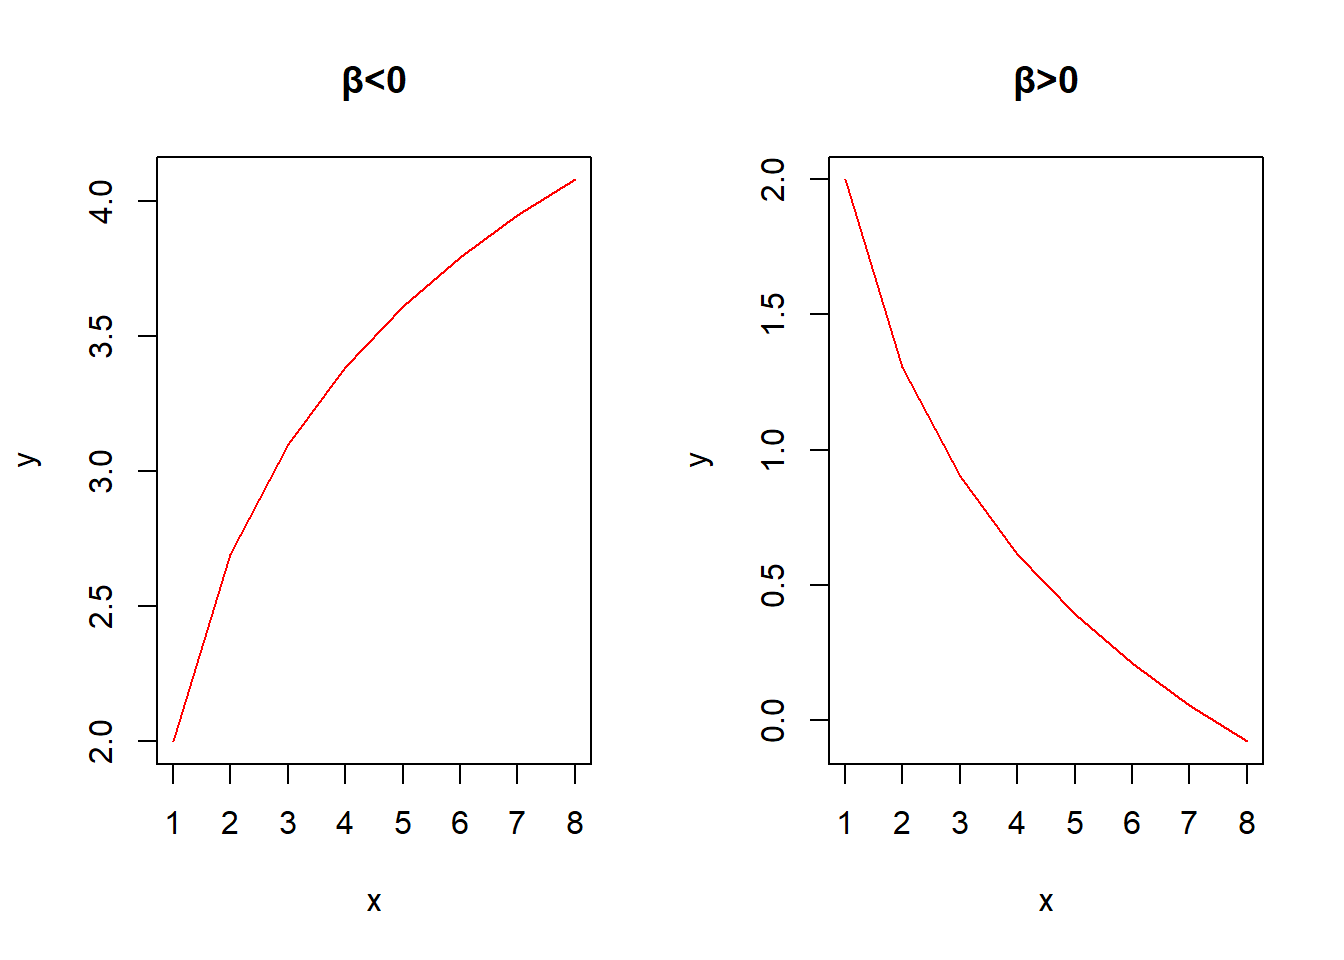
\includegraphics[width=1\linewidth,height=0.4\textheight]{bookdown_files/figure-latex/unnamed-chunk-49-1}

\begin{itemize}
\tightlist
\item
  指数曲线
\end{itemize}

基本形式:

\[y=\alpha^{\beta x}\]

线性化方法:两端取对数得:\(lny=ln\alpha+\beta x,y'=lny\),则有\(y'=ln\alpha+\beta x\)

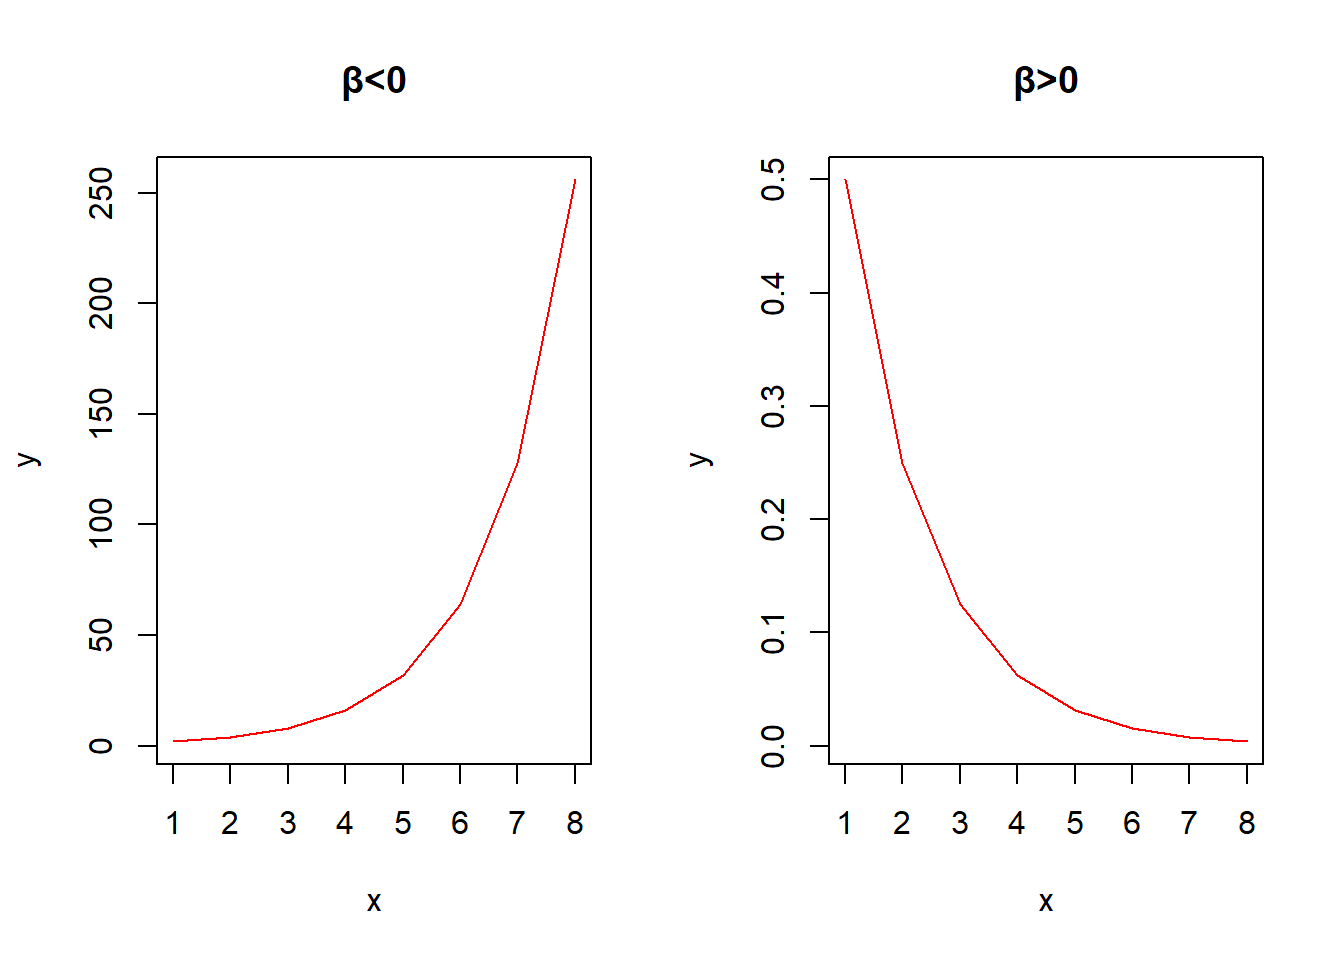
\includegraphics[width=1\linewidth,height=0.4\textheight]{bookdown_files/figure-latex/unnamed-chunk-50-1}

\begin{itemize}
\tightlist
\item
  S型曲线
\end{itemize}

基本形式:

\[y=\frac{1}{\alpha+\beta e^{-x}}\]

线性化方法:令\(y'=1/y,x'=e^{-x}\),则有\(y'=\alpha+\beta x'\)

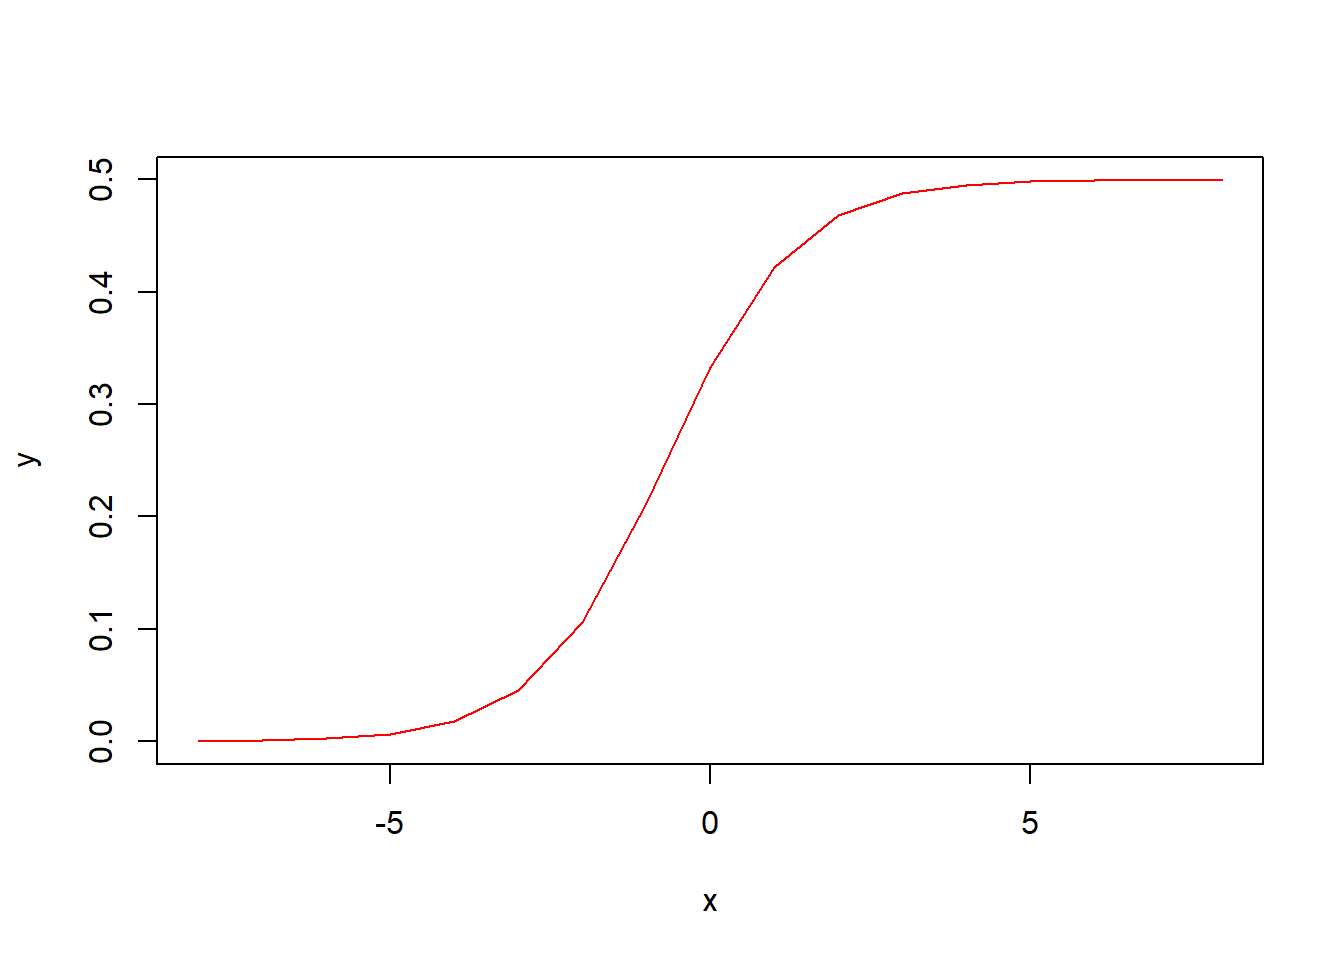
\includegraphics[width=1\linewidth,height=0.4\textheight]{bookdown_files/figure-latex/unnamed-chunk-51-1}

\hypertarget{ux5efaux7acbux56deux5f52ux6a21ux578b}{%
\section{建立回归模型}\label{ux5efaux7acbux56deux5f52ux6a21ux578b}}

得到描述因变量与一个或一个以上自变量之间关系的估计的回归方程。目的是建立一个基于最好自变量集合的模型。找到一个适合的描述变量关系之间关系的函数。选择模型应包含的变量。

\begin{quote}
\begin{itemize}
\tightlist
\item
  俭约的模型--用尽可能少的变量来提供足够精度的预测。
\item
  将不重要的变量除去更容易对模型进行解释。
\item
  发生多重共线性的可能变小。
\end{itemize}
\end{quote}

\textbf{变量选择Variable Selection}

\begin{quote}
有些变量的作用不是很大,SSE 不会随着变量个数的增加而增加,但MSE=SSE/(n-k-1)有可能会随着变量个数的增加而增加。最小的MSE可作为最优变量选择的一个准则,但需考虑所有子集 (\(2^p\)个)。
\end{quote}

\textbf{检验增加变量是否适宜的F统计}

\[F=\frac{SSE(x_1,x_2,\cdots,x_p)-SSE(x_1,x_2,\cdots,x_q,x_{q+1},\cdots,x_p)}{\frac{SSE(x_1,x_2,\cdots,x_q,x_{q+1},\cdots,x_p)}{n-p-1}}\]

\[F\sim F(p-q,n-p-1)\]

F越大,说明增加变量减少预测误差的效果越显著。

\textbf{变量选择过程}

\begin{quote}
\begin{itemize}
\tightlist
\item
  向前选择(Forward Selection)
\end{itemize}
\end{quote}

\begin{enumerate}
\def\labelenumi{\arabic{enumi}.}
\item
  从没有自变量的模型开始。
\item
  如果所有的F统计量的p-值大于预先设定的终止值,说明增加任一变量效果不显著,停止。
\item
  否则,加入具有最大F统计量值的变量。
\item
  重新回归, Go to Step 2。
\end{enumerate}

\begin{quote}
\begin{itemize}
\tightlist
\item
  后向消元(Backward Elimination)
\end{itemize}
\end{quote}

\begin{enumerate}
\def\labelenumi{\arabic{enumi}.}
\item
  从包含所有自变量的模型开始。
\item
  如果所有的F统计量的p-值小于预先设定的终止值,说明减少任一变量效果显著,停止。
\item
  否则,删除具有最小F统计量值的变量。
\item
  重新回归, Go to Step 2。
\end{enumerate}

\begin{quote}
\begin{itemize}
\tightlist
\item
  逐步回归(Stepwise regression procedure):向前选择和后向消元的结合。
\end{itemize}
\end{quote}

1.先检查是否有变量需从模型中删除。

2.再检查增加一个变量是否能改善模型。

3.重复以上过程。

注意: \(\alpha\)进\(\leq \alpha\)出,否则F进\textless F\textless F出,会导致无限循环。

\begin{quote}
\begin{itemize}
\tightlist
\item
  最佳子集回归(Best-subset approach):对所有可能的自变量组合进行估计。找出具有最大的修正判定系数\(adj.R^2\)和最小的估计误差标准差\(s_{\epsilon}\)。
\end{itemize}
\end{quote}

\hypertarget{ux56deux5f52ux4e2dux7684ux5e38ux89c1ux9519ux8bef}{%
\section{回归中的常见错误}\label{ux56deux5f52ux4e2dux7684ux5e38ux89c1ux9519ux8bef}}

(1)没有检验线性关系假设

\begin{quote}
\begin{itemize}
\tightlist
\item
  画散点图。
\item
  如果不是线性的,检验其它非线性。
\item
  用线性关系描述非线性关系会引起误导。
\end{itemize}
\end{quote}

(2)只看结果不看图表

\begin{quote}
\begin{itemize}
\tightlist
\item
  要将画散点图作为回归分析的一部分。
\item
  检验回归直线与实际观测值间的关系。
\item
  对自动回归来说这一步更为重要。
\end{itemize}
\end{quote}

(3)用回归系数判定变量的重要性

\begin{quote}
\begin{itemize}
\tightlist
\item
  回归系数依赖于自变量的量纲,因此系数的大小与变量的重要性无关。
\item
  例如,将秒变为微秒没有改变任何事实,但是变量的系数却有所改变。
\end{itemize}
\end{quote}

(4)没有确定置信区间

\begin{quote}
\begin{itemize}
\tightlist
\item
  观察值是随机样本,所以回归结果有一定随机性。
\item
  不确定置信区间,不可能理解参数的真正含义。
\end{itemize}
\end{quote}

(5)没有计算判定系数

\begin{quote}
\begin{itemize}
\tightlist
\item
  没有\(R^2\),很难确定多少变异是由回归解释的。
\item
  即使\(R^2\)看起来很好,安全起见还应做F-test。
\end{itemize}
\end{quote}

(6)错误解释相关系数

\begin{quote}
\begin{itemize}
\tightlist
\item
  判定系数是\(R^2\)。
\item
  相关系数是R。
\item
  \(R^2\)给出变异由回归解释的百分比,不是R。
\item
  如:R =0.5,\(R^2\)=0.25------回归解释了25\%的变异,不是50\%。
\end{itemize}
\end{quote}

(7)使用强相关的自变量

\begin{quote}
\begin{itemize}
\tightlist
\item
  模型同时包括两强相关的自变量会降低回归模型的显著性。
\item
  要尽可能的了解自变量间的关系。
\end{itemize}
\end{quote}

(8)用回归模型预测观测值范围之外的区域

\begin{quote}
\begin{itemize}
\tightlist
\item
  回归是基于某一特定观测样本的。
\item
  在样本观测值范围内能提供较为精确的估计。
\end{itemize}
\end{quote}

(9)观测值取值范围太小

\begin{quote}
\begin{itemize}
\tightlist
\item
  回归只有在观测值取值范围附近预测的结果比较好。
\item
  如果不在常用的范围内取值,回归模型用处不大。
\end{itemize}
\end{quote}

(10)包括太多的自变量

\begin{quote}
\begin{itemize}
\tightlist
\item
  变量越多的模型不一定越好。
\item
  有可能出现多重共线性。
\end{itemize}
\end{quote}

(11)认为好的预测变量是好的控制变量,相关关系不一定因果关系:A与B相关,并不意味着可以通过改变A来控制B。

(12)线性回归结果会给人以误导

\begin{quote}
\begin{itemize}
\tightlist
\item
  为了提供一个简练的总结,回归过程中舍弃了一些信息。
\item
  有时一些重要的特征也舍弃了------看图形表示可以告诉我们是否有问题。
\end{itemize}
\end{quote}

\hypertarget{logistic-ux56deux5f52}{%
\section{Logistic 回归}\label{logistic-ux56deux5f52}}

Logistic回归提出的目的是为了解决二值化数据的回归问题。那么为什么简单线性回归模型不适合二值化数据的回归呢?详细原因可见如下图。

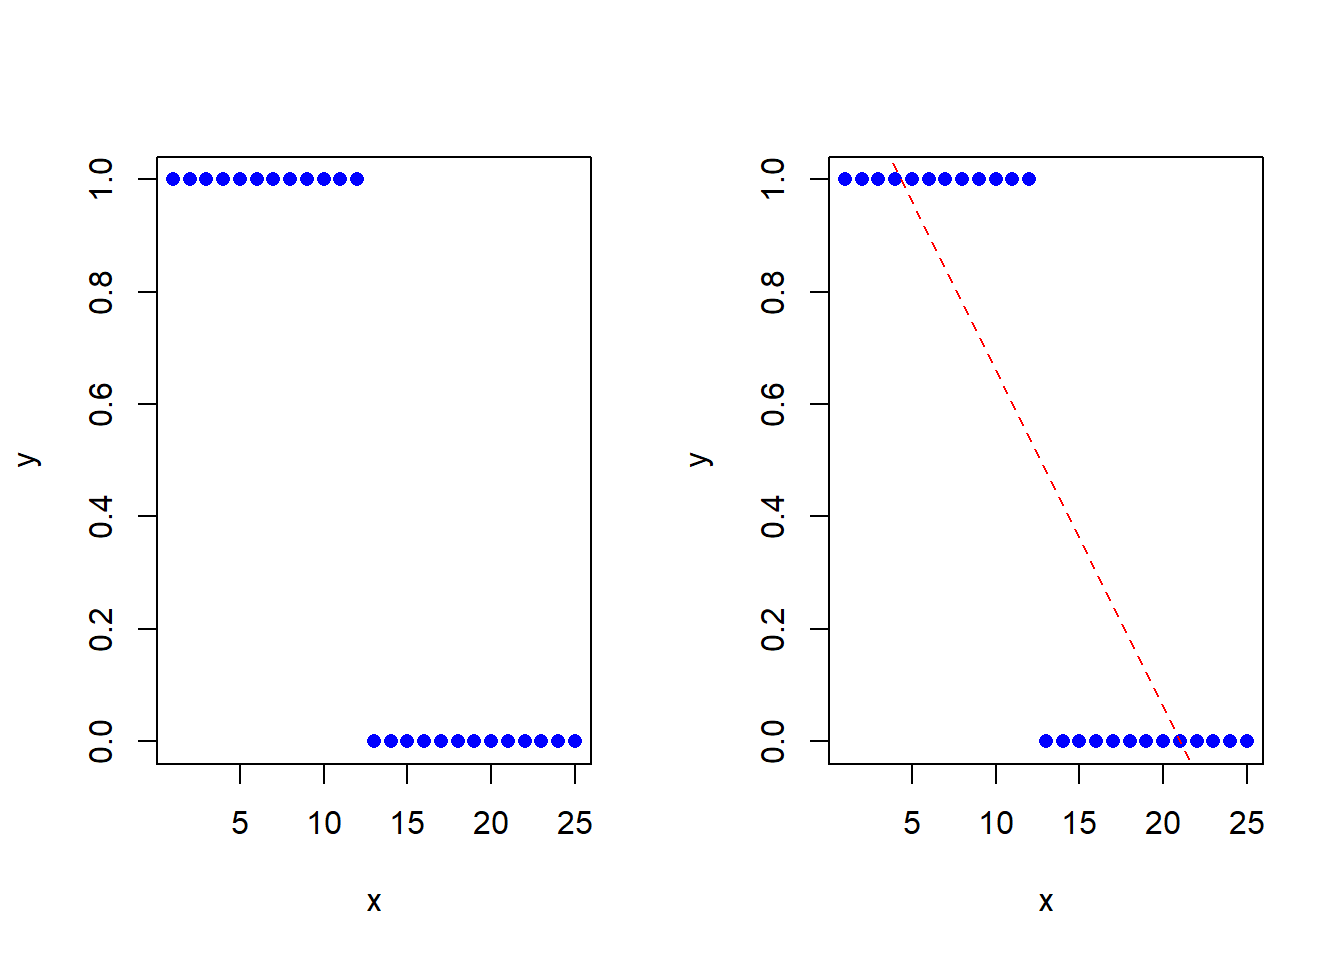
\includegraphics[width=1\linewidth,height=0.4\textheight]{bookdown_files/figure-latex/unnamed-chunk-52-1}

二值化变量是``yes''或者``no''的数据。可以被编码为1和0,也就是说不会有其他的变异数值。所以对于这种情况模型的要求是:模型的边界为0和1,模型可以输出的是一个在这类或者另一类的概率。我们想要的是一个实际值落入这类或者另一类的概率大小。而理想的模型是很好的估计0和1,或者换句话说,结果是0或1。所以解决方案就是Logistic回归。

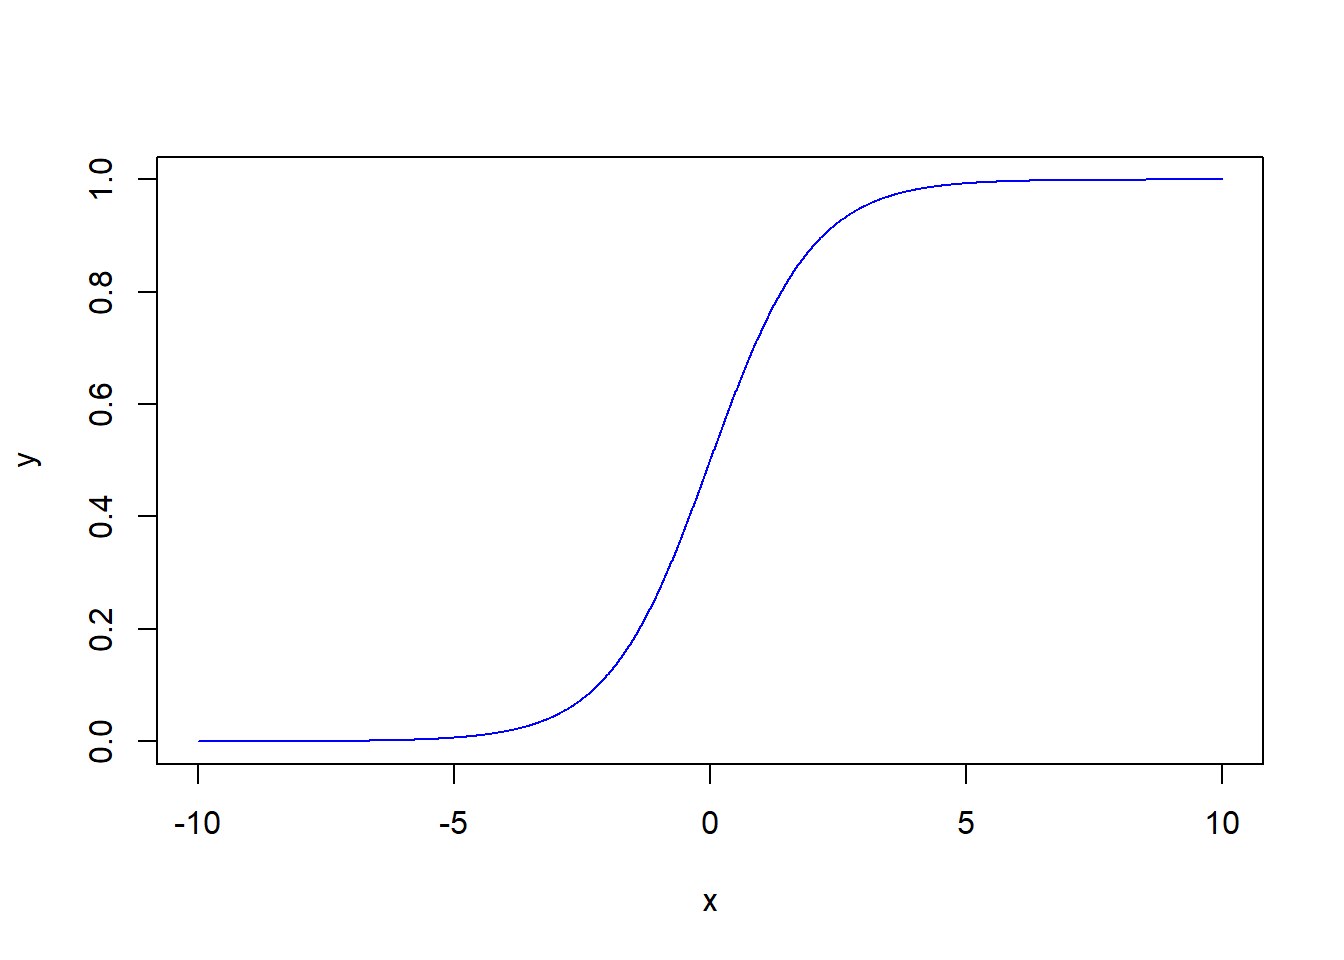
\includegraphics[width=1\linewidth,height=0.4\textheight]{bookdown_files/figure-latex/unnamed-chunk-53-1}

Logistic的基本形式为

\[\pi_i'=ln(\frac{\pi_i}{1-\pi_i})=\beta_0+\beta_1x_i\]

通过观测值估计\(n_i\)的概率\(p_i\),并且用\(ln(\frac{p_i}{1-p_i})\)估计。

典型案例:城市增长问题,城市化预测模拟,

\textbf{常见的问题}

\begin{quote}
\begin{itemize}
\tightlist
\item
  都有一个二值化(或分类)变量:
\item
  都涉及到预测的思想机会,概率,比例或百分比。
\item
  不像其他的预测情况,y值是有界的。
\end{itemize}
\end{quote}

\textbf{Logistic 回归与简单线性回归}

\begin{quote}
logistic回归是一种统计技术,可以用二值化变量问题中。回归虽有相似之处,但它不同于普通最小二乘法。识别重要和相似之处是两种技术的区别。
\end{quote}

\hypertarget{cluster}{%
\chapter{Cluster Analysis}\label{cluster}}

本篇是第十章,内容是聚类分析。由于之后的几章是典型的分析方法。而且在14章的案例里面可能不会体现,所以内容里会渗透较多的R语言操作。

\hypertarget{ux591aux5143ux5206ux5e03ux57faux672cux6982ux5ff5}{%
\section{多元分布基本概念}\label{ux591aux5143ux5206ux5e03ux57faux672cux6982ux5ff5}}

在研究实际问题的时候,我们经常遇到的是多变量的问题,由于指标间相互不独立,单独割裂开来分别研究分析,不能从整体上把握所研究问题的实质。所以我们必须对多元变量及其分布进行统计和分析,在地学领域这种问题比比皆是,这里就不展开阐述了,接下来是一堆纯数学概念,数学恐惧者慎入,这部分的重点应该是关于协方差矩阵。一般来说,假设所研究的问题有p个指标,进行了n次独立观测,得到了np个数据。那么对于单次独立观测,我们定义随机向量(Random Vector)为:\(x=(x_1,x_2,\cdots,x_p)'\),其概率分布函数定义为

\[F(a_1,a_2,\cdots,a_p)=P(x_1\le a_1,x_2\le a_2,\cdots,x_p\le a_p)\]

\textbf{分布函数的性质}

\begin{quote}
\begin{itemize}
\tightlist
\item
  非降的右连续函数
\item
  分布函数的取值范围为{[}0,1{]},即\(0\le F(a_1,a_2,\cdots,a_p)\le 1\)
\item
  分布函数当变量取值为无穷大时,函数值收敛到1,即\(F(\infty,\infty,\cdots,\infty)=1\)
\end{itemize}
\end{quote}

\textbf{多元概率密度函数}

随机向量\(x=(x_1,x_2,\cdots,x_p)'\)的分布函数可以表示为

\[F(a_1,a_2,\cdots,a_p)=P(x_1\le a_1,x_2\le a_2,\cdots,x_p\le a_p)=\int_{-\infty}^{a_1}\cdots\int_{-\infty}^{a_p}f(x_1,x_2,\cdots,x_p)dx_1\cdots dx_p\]
则称\(x=(x_1,x_2,\cdots,x_p)'\)为连续型随机变量,称\(f(x_1,x_2,\cdots,x_p)\)为其多元概率密度函数。若\(F(a_1,a_2,\cdots,a_p)\)在点\((x_1,x_2,\cdots,x_p)\)连续,则\(f(x_1,x_2,\cdots,x_p)=\frac{\partial^p}{\partial x_1\partial x_2\cdots\partial x_p}F(x_1,x_2,\cdots,x_p)\)且有\(1\ge F(x_1,x_2,\cdots,x_p)\ge 0,\int_{-\infty}^{a_1}\cdots\int_{-\infty}^{a_p}f(x_1,x_2,\cdots,x_p)dx_1\cdots dx_p=1\)。

\textbf{数学期望}

定义

\[\begin{bmatrix} x_{11} & x_{12} & \cdots & x_{1q} \\ x_{21} & x_{22} & \cdots & x_{2q} \\ \vdots & \vdots &  & \vdots \\ x_{p1} & x_{p2} & \cdots & x_{pq} \end{bmatrix}\]
是由随机变量构成的随机矩阵,定义X的数学期望为

\[\begin{bmatrix} E(x_{11}) & E(x_{12}) & \cdots & E(x_{1q}) \\ E(x_{21}) & E(x_{22}) & \cdots & E(x_{2q}) \\ \vdots & \vdots &  & \vdots \\ E(x_{p1}) & E(x_{p2}) & \cdots & E(x_{pq}) \end{bmatrix}\]
特别当q=1时,便可得到随机向量\((x_1,x_2,\cdots,x_p)'\)的数学期望为\(E(x)=(E(x_1),E(x_2),\cdots,E(x_p))'\)

\textbf{协方差矩阵}

设\(x=(x_1,x_2,\cdots,x_p)'\)和\(y=(y_1,y_2,\cdots,y_q)'\)分别为p维和q维随机向量,则其协方差矩阵为

\[E\begin {bmatrix} \begin {pmatrix} x-E(x_1) \\ x-E(x_2) \\ \vdots \\ x-E(x_p) \end{pmatrix} (y-E(y_1),(y-E(y_2),\cdots,(y-E(y_q) \end {bmatrix}\]

\[=\begin {pmatrix} cov(x_1,y_1) & cov(x_1,y_2) & \cdots & cov(x_1,y_q) \\ cov(x_2,y_1) & cov(x_2,y_2) & \cdots & cov(x_2,y_q) \\ \vdots & \vdots &  & \vdots \\ cov(x_p,y_1) & cov(x_p,y_2) & \cdots & cov(x_p,y_q) \end {pmatrix}=cov(X,Y)\]

\(x=(x_1,x_2,\cdots,x_p)'\)的协方差矩阵为

\[\Sigma=Var(x)=\begin {pmatrix} var(x_1) & cov(x_1,x_2) & \cdots & cov(x_1,x_p) \\ cov(x_2,x_1) & var(x_2) & \cdots & cov(x_2,x_p) \\ \vdots & \vdots &  & \vdots \\ cov(x_p,x_1) & cov(x_p,x_2) & \cdots & var(x_p) \end {pmatrix}\]

随机向量X的协方差矩阵Σ是非负定矩阵。设A是常数矩阵,b为常数向量,则
\(Var(AX+b)=AV(X)A'=A\Sigma A'\)。若\((x_1,x_2,\cdots,x_p)'\)的分量相互独立,则协方差矩阵除主对角线上的元素外均为零,即
\(\Sigma=Var(x)=\begin {pmatrix} var(x_1) & 0 & \cdots & 0 \\ 0 & var(x_2) & \cdots & 0 \\ \vdots & \vdots & & \vdots \\ 0 & 0 & \cdots & var(x_p) \end {pmatrix}\)

\textbf{相关系数矩阵}

若\(x=(x_1,x_2,\cdots,x_p)'\)和\(y=(y_1,y_2,\cdots,y_q)'\)分别是p维和q维随机向量,则其相关系数矩阵为

\[\rho (x,y)=\begin {pmatrix} \rho (x_1,y_1) & \rho (x_1,y_2) & \cdots & \rho (x_1,y_q) \\ \rho (x_2,y_1) & \rho (x_2,y_2) & \cdots & \rho (x_2,y_q) \\ \vdots & \vdots &  & \vdots \\ \rho (x_p,y_1) & \rho (x_p,y_2) & \cdots & \rho (x_p,y_q) \end {pmatrix}\]
若\(\rho (x,y)=0\),两随机向量相互独立。

\hypertarget{ux6570ux636eux7684ux53d8ux6362ux5904ux7406}{%
\section{数据的变换处理}\label{ux6570ux636eux7684ux53d8ux6362ux5904ux7406}}

数据变换是将原始数据矩阵中的每个元素按照某种特定的运算把它变成为一个新值,而且数值的变化不依赖于原始数据集合中其它数据的新值。事实上多元数据的变换处理通常是为了消除不同量纲的差异。较常用的数据变换如下:

\begin{itemize}
\tightlist
\item
  中心化变换
\end{itemize}

中心化变换是一种坐标轴平移处理方法,它是先求出每个变量的样本平均值,再从原始数据中减去该变量的均值,就得到中心化变换后的数据。设原始观测数据矩阵为:

\[X= \begin{bmatrix} x_{11} & x_{12} & \cdots & x_{1q} \\ x_{21} & x_{22} & \cdots & x_{2q} \\ \vdots & \vdots &  & \vdots \\ x_{n1} & x_{n2} & \cdots & x_{nq} \end{bmatrix} \]
\[ x_{ij}^*=x_{ij}-\bar x_j (i=1,2,\cdots,n;j=1,2,\cdots,p) \]

中心化变换的结果是使每列数据之和均为0,即每个变量的均值为0,而且每列数据的平方和是该列变量样本方差的(n-1)倍,任何不同两列数据之交叉乘积是这两列变量样本协方差的(n-1)倍,所以这是一种很方便地计算方差与协方差的变换。

\begin{itemize}
\tightlist
\item
  极差规格化变换
\end{itemize}

极差规格化变换是从数据矩阵的每一个变量中找出其最大值和最小值,这两者之差称为极差,然后从每个变量的每个原始数据中减去该变量中的最小值,再除以极差,就得到规格化数据。

\[x_{ij}^*=\frac{x_{ij}-min_{k=1,2,\cdots,n} (x_{kj})}{R_j} (i=1,2,\cdots,n;j=1,2,\cdots,p)\]
\[R_j= max_{i=1,2,\cdots,n} (x_{ij})-min_{i=1,2,\cdots,n} (x_{ij}),0\le  x_{ij}^*\le 1\]
经过极差规格化变换后,数据矩阵中每列即每个变量的最大数值为1,最小数值为0,其余数据取值均在0和1之间;并且变换后的数据都不再具有量纲,便于不同的变量之间的比较。

\begin{itemize}
\tightlist
\item
  标准化变换
\end{itemize}

标准化变换首先对每个变量进行中心化变换,然后用该变量的标准差进行标准化。

\[x_{ij}^*=\frac{(x_{ij}-\bar x)}{S_j} (i=1,2,\cdots,n;j=1,2,\cdots,p)\]

\[S_j=\sqrt{\frac{1}{n-1}\sum_{i=1}^n(x_{ij}-\bar x_j)^2}\]

经过标准化变换处理后,数据矩阵中每列数据即每个变量的平均值为0,方差为1,且不再具有量纲,便于不同变量之间的比较。变换后,数据矩阵中任何两列数据乘积之和是所对应的两个变量相关系数的(n-1)倍,所以这是一种很方便地计算相关矩阵的变换。

\begin{itemize}
\tightlist
\item
  对数变换
\end{itemize}

对数变换是将各个原始数据取对数,将原始数据的对数值作为变换后的新值。

\[x_{ij}^*=log(x_{ij})\]

\hypertarget{ux805aux7c7bux5206ux6790}{%
\section{聚类分析}\label{ux805aux7c7bux5206ux6790}}

聚类分析是一种分类技术。与多元分析的其他方法相比,该方法较为粗糙,理论上还不完善,但应用方面取得了很大成功。与回归分析、判别分析一起被称为多元分析的三大方法。

\textbf{聚类的目的}------根据已知数据( 一批观察个体的许多观测指标),按照一定的数学公式计算各观察个体或变量(指标)之间亲疏关系的统计量(距离或相关系数等)。 根据某种准则(最短距离法、最长距离法、中间距离法、重心法等),使同一类内的差别较小,而类与类之间的差别较大,最终将观察个体或变量分为若干类。

\textbf{聚类的种类}------根据分类的方法可将聚类分析分为:系统聚类、快速聚类、有序聚类。根据分类的对象可将聚类分析分为:Q型------样品聚类clustering for individuals;R型------指标聚类clustering for variables。

\textbf{数据结构}

\begin{longtable}[]{@{}lcccr@{}}
\toprule
individuals & \(X_1\) & \(X_2\) & \(\cdots\) & \(X_l\)\tabularnewline
\midrule
\endhead
1 & 28 & 1.0 & \(\cdots\) & 114\tabularnewline
2 & 29 & 2.0 & \(\cdots\) & 117\tabularnewline
\(\cdots\) & \(\cdots\) & \(\cdots\) & \(\cdots\) & \(\cdots\)\tabularnewline
i & \(x_{i1}\) & \(x_{i2}\) & \(\cdots\) & \(x_{il}\)\tabularnewline
\(\cdots\) & \(\cdots\) & \(\cdots\) & \(\cdots\) & \(\cdots\)\tabularnewline
47 & 15 & 8 & \(\cdots\) & 64\tabularnewline
48 & 16 & 7.5 & \(\cdots\) & 65\tabularnewline
\(\cdots\) & \(\cdots\) & \(\cdots\) & \(\cdots\) & \(\cdots\)\tabularnewline
n & \(x_{n1}\) & \(x_{n2}\) & \(\cdots\) & \(x_{nl}\)\tabularnewline
\bottomrule
\end{longtable}

\hypertarget{ux6837ux54c1ux95f4ux4eb2ux758fux7a0bux5ea6ux7684ux6d4bux5ea6}{%
\section{样品间亲疏程度的测度}\label{ux6837ux54c1ux95f4ux4eb2ux758fux7a0bux5ea6ux7684ux6d4bux5ea6}}

\textbf{样品间亲疏程度的测度:} 研究样品或变量的亲疏程度的数量指标有两种,一种叫相似系数,性质越接近的变量或样品,它们的相似系数越接近于1,而彼此无关的变量或样品它们的相似系数则越接近于0,相似的为一类,不相似的为不同类;另一种叫距离,它是将每一个样品看作p维空间的一个点,并用某种度量测量点与点之间的距离,距离较近的归为一类,距离较远的点属于不同的类。变量之间的聚类即R型聚类分析,常用相似系数来测度变量之间的亲疏程度。而样品之间的聚类即Q型聚类分析,则常用距离来测度样品之间的亲疏程度。

\textbf{距离:}假使每个样品有p个变量,则每个样品都可以看成p维空间中的一个点,n个样品就是p维空间中的n个点,则第i样品与第j样品之间的距离记为\(d_{ij}\)。

\textbf{定义距离的准则:}定义距离要求满足第i个和第j个样品之间的距离如下四个条件(距离可以自己定义,只要满足距离的这四个条件)。

\begin{quote}
\begin{itemize}
\tightlist
\item
  \(d_{ij}\ge 0\)对一切的i和j成立;
\item
  \(d_{ij}=0\)当且仅当\(x_i=x_j\)成立;
\item
  \(d_{ij}=d_{ji}\)对一切的i和j成立;
\item
  \(d_{ij}\le d_{ik}+d_{kj}\)对于一切的i和j成立。
\end{itemize}
\end{quote}

\textbf{常用距离}

设\(x_i=(x_{i1},x_{i1},\cdots,x_{ip})'\)和\(x_j=(x_{j1},x_{j1},\cdots,x_{jp})'\)是第i和j个样品的观测值,则二者之间的常用距离公式如下。

明氏距离(Minkowski):

\[d_{ij}=(\sum_{k=1}^p \left |x_{ik}-x_{jk}|^q\right)^{\frac{1}{q}}\]

欧氏距离:

\[d_{ij}=\sqrt{\sum_{k=1}^p(x_{ik}-x_{jk})^2}\]

绝对距离:

\[d_{ij}=\sum_{k=1}^p|x_{ik}-x_{jk}|\]

Chebychev距离:

\[d_{ij}=max_{k=1}^p|x_{ik}-x_{jk}|\]

\textbf{明氏距离主要有以下两个缺点}
明氏距离的值与各指标的量纲有关,而各指标计量单位的选择有一定的人为性和随意性,各变量计量单位的不同不仅使此距离的实际意义难以说清,而且,任何一个变量计量单位的改变都会使此距离的数值改变从而使该距离的数值依赖于各变量计量单位的选择。明氏距离的定义没有考虑各个变量之间的相关性和重要性。实际上,明氏距离是把各个变量都同等看待,将两个样品在各个变量上的离差简单地进行了综合。

兰氏距离(Lance \& Williams):这是兰思和维廉姆斯(Lance \& Williams)所给定的一种距离,其计算公式为:

\[d_{ij}(L)=\sum_{k=1}^p\frac{|x_{ik}-x_{jk}|}{x_{ik}+x_{jk}}\]

这是一个自身标准化的量,由于它对大的奇异值不敏感,这样使得它特别适合于高度偏倚的数据。虽然这个距离有助于克服明氏距离的第一个缺点,但它也没有考虑指标之间的相关性。

马氏距离(Mahalanobis):这是印度著名统计学家马哈拉诺比斯(P.C. Mahalanobis)所定义的一种距离,其计算公式为:

\[d_{ij}^2=(x_i-x_j)'\Sigma^{-1}(x_i-x_j)\]

\(\Sigma\)表示观测变量之间的协方差短阵。在实践应用中,若总体协方差矩阵\(\Sigma\)未知,则可用样本协方差矩阵作为估计代替计算。马氏距离又称为广义欧氏距离。显然,马氏距离与上述各种距离的主要不同就是马氏距离考虑了观测变量之间的相关性。如果假定各变量之间相互独立,即观测变量的协方差矩阵是对角矩阵,则马氏距离就退化为用各个观测指标的标准差的倒数作为权数进行加权的欧氏距离。因此,马氏距离不仅考虑了观测变量之间的相关性,而且也考虑到了各个观测指标取值的差异程度。

斜交空间距离:由于各变量之间往往存在着不同的相关关系,用正交空间的距离来计算样本间的距离易变形,所以可以采用斜交空间距离。

\[d_{ij}=[\frac{1}{p^2}\sum_{h=1}^p\sum_{k=1}^p(x_{ih}-x_{jh})(x_{ik}-x_{jk})r_{hk}]^{\frac{1}{2}}\]
当各变量之间不相关时,斜交空间退化为欧氏距离。

配合距离

\[X_1=(V,Q,S,T,K) X_2=(V,M,S,F,K)\]
\[d_{12}=\frac{m_1}{m_1+m_2}=\frac{no-pairs}{pairs+no-pairs}=\frac{2}{2+3}=\frac{2}{5}\]

适用于分类变量,尤其是名义尺度变量。

\textbf{相似系数}

研究样品间的关系常用距离,研究指标间的关系常用相似系数。相似系数常用的有夹角余弦和相关系数。

夹角余弦(Cosine):夹角余弦是从向量集合的角度所定义的一种测度变量之间亲疏程度的相似系数。设在n维空间的向量
\[x_i=(x_{1i},x_{2i},\cdots,x_{ni})',x_j=(x_{1j},x_{2j},\cdots,x_{nj})'\]。

\[c_{ij}=\cos \alpha_{ij}=\frac{\sum_{k=1}^nx_{ki}x_{kj}}{\sqrt{\sum_{k=1}^nx_{ki}^2\sum_{k=1}^nx_{kj}^2}},d_{ij}^2=1-c_{ij}^2\]

相关系数是将数据标准化后的夹角余弦

\[x_i=(x_{1i},x_{2i},\cdots,x_{ni})',x_j=(x_{1j},x_{2j},\cdots,x_{nj})'\]

\[c_{ij}=\frac{\sum_{k=1}^n(x_{ki}-\bar x_i)(x_{kj}-\bar x_j)}{\sqrt{\sum_{k=1}^n(x_{ki}-\bar x_i)^2\sum_{k=1}^n(x_{kj}-\bar x_j)^2}}\]

\textbf{距离和相似系数选择的原则}

一般说来,同一批数据采用不同的亲疏测度指标,会得到不同的分类结果。产生不同结果的原因,主要是由于不同的亲疏测度指标所衡量的亲疏程度的实际意义不同,也就是说,不同的亲疏测度指标代表了不同意义上的亲疏程度。因此我们在进行聚类分析时,应注意亲疏测度指标的选择。通常,选择亲疏测度指标时,应注意遵循的基本原则主要有:所选择的亲疏测度指标在实际应用中应有明确的意义。如在经济变量分析中,常用相关系数表示经济变量之间的亲疏程度。适当地考虑计算工作量的大小。如对大样本的聚类问题,不适宜选择斜交空间距离,因采用该距离处理时,计算工作量太大。

亲疏测度指标的选择要综合考虑已对样本观测数据实施了的变换方法和将要采用的聚类分析方法。如在标准化变换之下,夹角余弦实际上就是相关系数;又如若在进行聚类分析之前已经对变量的相关性作了处理,则通常就可采用欧氏距离,而不必选用斜交空间距离。此外,所选择的亲疏测度指标,还须和所选用的聚类分析方法一致。如聚类方法若选用离差平方和法,则距离只能选用欧氏距离。

样品间或变量间亲疏测度指标的选择是一个比较复杂且带主观性的问题,我们应根据研究对象的特点作具体分析,以选择出合适的亲疏测度指标。实践中,在开始进行聚类分析时,不妨试探性地多选择几个亲疏测度指标,分别进行聚类,然后对聚类分析的结果进行对比分析,以确定出合适的亲疏测度指标。

\hypertarget{ux7c7bux4e0eux7c7bux4e4bux95f4ux7684ux8dddux79bb}{%
\section{类与类之间的距离}\label{ux7c7bux4e0eux7c7bux4e4bux95f4ux7684ux8dddux79bb}}

\begin{quote}
\begin{itemize}
\tightlist
\item
  最短距离法(Nearest Neighbor)
\item
  最长距离法(Furthest Neighbor)
\item
  重心法(Centroid method)
\item
  类平均法(average linkage)------组间连接法(Between-groups Linkage)和组内连接法(Within-groups Linkage)
\item
  Ward离差平方和法(Ward's minimumvariance method)
\end{itemize}
\end{quote}

\hypertarget{ux7cfbux7edfux805aux7c7bhierarchical-clustering-method}{%
\section{系统聚类(hierarchical clustering method)}\label{ux7cfbux7edfux805aux7c7bhierarchical-clustering-method}}

\textbf{系统聚类的步骤}

(1) 开始将n个样品各作为一类。

(2) 根据样品的特征,选择合适的距离公式,计算n个样品两两之间的距离,构成距离矩阵。

(3) 选择距离矩阵中最小的非对角线元素\(d_{pq}\),将相应的两类\(G_p\)和\(G_q\)合并为一新类\(G_r={G_p,G_q}\)。

(4) 利用递推公式计算新类与当前各类的距离。 分别删除原矩阵的第p,q行和第p,q列,并新增一行和一列添上的结果,产生新的距离矩阵。

(5) 再合并、计算,直至只有一类为止。

(6) 画聚类图,解释。

\begin{itemize}
\tightlist
\item
  最短距离法
\end{itemize}

定义距离:\(D_{pq}=Min{d_{ij}:x_i\in G_p,x_j\in G_q}\),假设第p类和第q类合并成第r类,第r类与其它各旧类的距离按最短距离法为递推公式:

\[D_{rl}=Min{D_{pl},D_{ql}}\] \[l\neq p,q\]

\begin{itemize}
\tightlist
\item
  最长距离法
\end{itemize}

定义距离:\(D_{pq}=Max{d_{ij}:x_i\in G_p,x_j\in G_q}\),假设第p类和第q类合并成第r类,第r类与其它各旧类的距离按最长距离法为递推公式:

\[D_{rl}=Max{D_{pl},D_{ql}}\] \[l\neq p,q\]

\begin{itemize}
\tightlist
\item
  中间距离法
\end{itemize}

递推公式:

\[D_{lr}^2=\frac{1}{2}D_{lp}^2+\frac{1}{2}D_{lq}^2-\frac{1}{4}D_{pq}^2\]

\[D_{kr}^2=\frac{1}{2}D_{kp}^2+\frac{1}{2}D_{kq}^2+\beta D_{pq}^2,-\frac{1}{4}< \beta < 0\]

\begin{itemize}
\tightlist
\item
  可变方法
\end{itemize}

如果让中间距离法的递推公式前两项的系数也依赖于β,则递推公式为:

\[D_{kr}^2=\frac{1-\beta}{2}(D_{kp}^2+D_{kq}^2)+\beta D_{pq}^2,\beta < 1\]

用上式作为递推公式的系统聚类法称为可变法。

\begin{itemize}
\tightlist
\item
  重心法
\end{itemize}

假设第p类和第q类合并成第r类,第r类与其它各旧类的距离按重心法为:

\[D_{rl}^2=\frac{n_p}{n_r}D_{pl}^2+\frac{n_q}{n_r}D_{ql}^2-\frac{n_pn_q}{n_r^2}D_{pq}^2\]

\begin{itemize}
\tightlist
\item
  类平均方法
\end{itemize}

类平均法定义类间的距离是两类间样品的距离的平均数,递推公式:

\[D_{rk}^2=\frac{n_pD_{kp}^2+n_qD_{kq}^2}{n_p+n_q}\]

\begin{itemize}
\tightlist
\item
  可变类平均法
\end{itemize}

类平均法的递推公式中,没有反映\(G_p\)类和\(G_q\)类的距离有多大,进一步将其改进,加入\(D_{pq}^2\),并给定系数\(\beta<1\), 则类平均法的递推公式改为:

\[D_{rl}^2=(1-\beta)\frac{n_pD_{pl}^2+n_qD_{ql}^2}{n_p+n_q}+\beta D_{pq}^2\]

用此递推公式进行聚类就是可变类平均法。递推公式由p类和q类与l类的距离的加权平均数、p类和q类的距离两项的加权和构成,\(\beta\)的大小根据哪项更重要而定。

\begin{itemize}
\tightlist
\item
  离差平方和法
\end{itemize}

类似于方差分析的想法,如果类分得恰当,同类内的样品之间的离差平方和应较小,而类间的离差平方和应当较大。当k固定时,选择使SST达到最小的分类。分类可能指数级增长,寻找最优难以完成。离差平方和法的思路:先让n个样品各自成一类,然后缩小一类,每缩小一类离差平方和就要增大,选择使SST增加最小的两类合并,直到所有的样品归为一类为止(局部最优)。定义距离为离差平方和的增量:\(D_{pq}=S_r^2-S_p^2-S_q^2\),其中\(S_r^2\)是由\(G_p\)和\(G_q\)合并成的\(G_r\)类的类内离差平方和。可以证明离差平方和的聚类公式为。

递推公式:

\[D_{rk}^2=\frac{n_k+n_p}{n_r+n_k}D_{pk}^2+\frac{n_k+n_q}{n_r+n_k}D_{qk}^2-\frac{n_k}{n_k+n_r}D_{pq}^2\]

以上聚类方法的计算步骤完全相同,仅类与类之间距离的定义不同。 Lance和Williams于1967年将其统一为:

\[D_{MJ}^2=\alpha_KD_{KJ}^2+\alpha_LD_{KJ}^2+\beta D_{KL}^2+\gamma|D_{KJ}^2-D_{KJ}^2|\]

\textbf{确定类的个数}

从系统聚类的计算机结果可以得到任何可能数量的类。但是,聚类的目的是要使各类之间的距离尽可能地远,而类中点的距离尽可能的近, 并且分类结果还要有令人信服的解释。往往做系统聚类的时候,大部分情况下我们都是依靠人的主观判断确定最后分类的个数。这里给出了一些统计方法来确定类的个数。

\begin{quote}
\begin{itemize}
\tightlist
\item
  给定阈值
\item
  通过观测聚类图, 给出一个合适的阈值T。要求类与类之间的距离要超过T值。 例如我们给定T=0.35, 当聚类时,类间的距离已经超过了0.35, 则聚类结束。
\item
  统计量\(R^2\)
\item
  总离差平方和的分解
\end{itemize}
\end{quote}

\[\begin{bmatrix} x_{11} & x_{12} & \cdots & x_{1p} \\ x_{21} & x_{22} & \cdots & x_{2p} \\ \vdots & \vdots &  & \vdots \\ x_{n1} & x_{n2} & \cdots & x_{np} \end{bmatrix}\]

\begin{quote}
\begin{itemize}
\tightlist
\item
  总离差平方和
\end{itemize}
\end{quote}

\[=(x_{11}-\bar x_1)^2+\cdots+(x_{n1}-\bar x_1)^2+\cdots+(x_{1p}-\bar x_p)^2+\cdots+(x_{np}-\bar x_p)^2\]

如果这些样本被分为两类

\[\begin{bmatrix} x_{11} & x_{12} & \cdots & x_{1p} \\ x_{21} & x_{22} & \cdots & x_{2p} \\ \vdots & \vdots &  & \vdots \\ x_{n_11} & x_{n_12} & \cdots & x_{n_1q} \end{bmatrix} \begin{bmatrix} x_{11} & x_{12} & \cdots & x_{1p} \\ x_{21} & x_{22} & \cdots & x_{2p} \\ \vdots & \vdots &  & \vdots \\ x_{n_21} & x_{n_22} & \cdots & x_{n_2p} \end{bmatrix}\]

一组离差平方和

\[=(x_{11}-\bar x_1^{(1)})^2+\cdots+(x_{n_11}-\bar x_1^{(1)})^2+\cdots+(x_{1p}-\bar x_p^{(1)})^2+\cdots+(x_{n_1p}-\bar x_p^{(1)})^2\]

二组离差平方和

\[=(x_{11}-\bar x_1^{(2)})^2+\cdots+(x_{n_11}-\bar x_1^{(2)})^2+\cdots+(x_{1p}-\bar x_p^{(2)})^2+\cdots+(x_{n_1p}-\bar x_p^{(2)})^2 \]

可以证明:总离差平方和=组内离差平方和+组间离差平方和。令T为总离差平方和,令\(P_G\)为分为G类的组内离差平方和。

统计量:

\[R^2=1-\frac{P_G}{T}\]

其中T是数据的总离差平方和, 是组内离差平方和。R²比较大,说明分G个类时组内离差平方和比较小,也就是说分G类是合适的。但是,分类越多,每个类的组内离差平方和就越小,\(R^2\)也就越大;所以我们只能取合适的G,使得\(R^2\)足够大,而G本身很小,随着G的增加,\(R^2\)的增幅不大。比如,假定分4类时,\(R^2\)=0.8;下一次合并分三类时,下降了许多,\(R^2\)=0.32,则分4类是合适的。

伪F统计量,伪F统计量的定义为

\[F=\frac{(T-P_G)/(G-1)}{P_G/(n-G)}\]

伪F统计量用于评价聚为G类的效果。如果聚类的效果好,类间的离差平方和相对于类内的离差平方和大,所以应该取伪F统计量较大而类数较小的聚类水平。

伪\(t^2\)统计量,伪t²统计量的定义为

\[t^2=\frac{B_{KL}}{(W_K+W_L)/(N_K+N_L-2)}\]

其中\(W_L\)和\(W_K\)分别是类内离差平方和,\(W_M\)是将K和L合并为第M类的离差平方和,\(B_{KL}=W_M-W_K-W_L\)为合并导致的类内离差平方和的增量。用它评价合并第K和L类的效果,伪\(t^2\)统计量大说明不应该合并这两类,应该取合并前的水平。

\hypertarget{ux5febux901fux805aux7c7bk-means-clustering-method}{%
\section{快速聚类(k-means clustering method)}\label{ux5febux901fux805aux7c7bk-means-clustering-method}}

\textbf{系统聚类法的缺陷}------系统聚类法是一种比较常用的聚类方法。然而当样本点数量十分庞大时,则是一件非常繁重的工作,聚类的计算速度也比较慢。比如在市场抽样调查中,有4万人就其对衣着的偏好作了回答,希望能迅速将他们分为几类。这时,用系统聚类法计算的工作量极大,作出的树状图也十分复杂,不便于分析。

\textbf{quick cluster method, k-means method:}也叫动态聚类、逐步聚类、迭代聚类、k-均值聚类,快速聚类适用于大型数据。

快速聚类(K-means)流程图

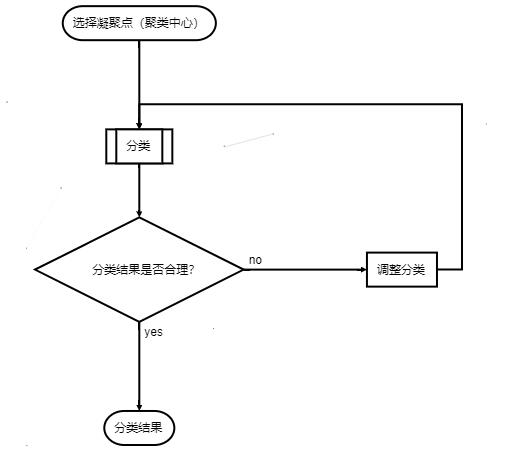
\includegraphics[width=1\linewidth,height=0.45\textheight]{fig/fig22}

用一个简单的例子来说明快速聚类法的工作过程。例如我们要把图中的点分成两类。 快速聚类的步骤:

(1)随机选取两个点\(x_1^{(1)}\)和\(x_2^{(1)}\)作为聚核。

(2)对于任何点\(x_k\),分别计算\(d(x_k,x_1^{(1)})\)和\(d(x_k,x_2^{(1)})\)

(3)若\(d(x_k,x_1^{(1)})< d(x_k,x_2^{(1)})\),则将\(x_k\)划为第一类,否则划给第二类。于是得图(b)的两个类。

(4)分别计算两个类的重心,则得\(x_1^{(2)}\)和\(x_2^{(2)}\),以其为新的聚核,对空间中的点进行重新分类,得到新分类。

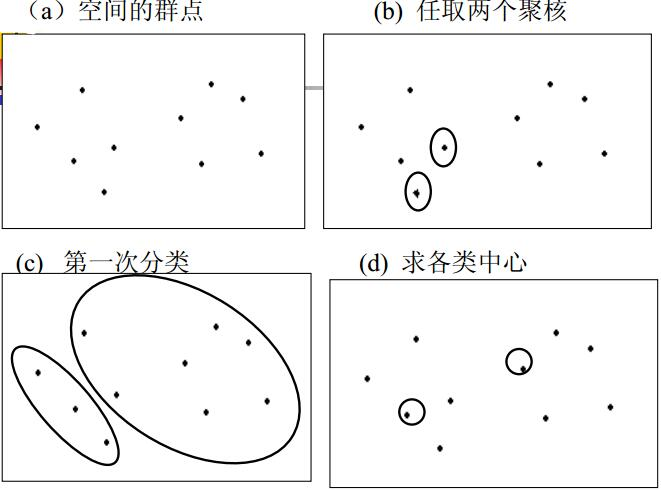
\includegraphics[width=1\linewidth,height=0.35\textheight]{fig/fig23}

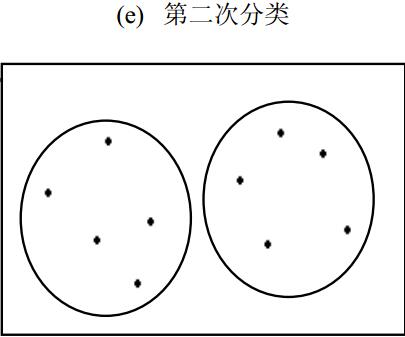
\includegraphics[width=0.8\linewidth,height=0.3\textheight]{fig/fig24}

\begin{itemize}
\tightlist
\item
  选择凝聚点
\end{itemize}

初始凝聚点(聚类种子、initial cluster seeds/clustercenters)就是一批有代表性的点,是欲形成类的中心。初始凝聚点的选择直接决定初始分类,对分类结果也有很大的影响,由于凝聚点的不同选择,其最终分类结果也将出现不同,故选择时要慎重。通常选择初始凝聚点的方法有:

人为选择,当人们对所欲分类的问题有一定了解时,根据经验,预先确定分类个数和初始分类,并从每一类中选择一个有代表性的样品作为凝聚点。将数据人为地分为A类,计算每一类的重心,就将这些重心作为凝聚点。

用密度法选择凝聚点。以某个正数d为半径,以每个样品为球心,落在这个球内的样品数(不包括作为球心的样品)就叫做这个样品的密度。计算所有样品点的密度后,首先选择密度最大的样品作为第一凝聚点,并且人为地确定一个正数D(一般D>d,常取D=2d)。然后选出次大密度的样品点,若它与第一个凝聚点的距离大于D,则将其作为第二个凝聚点;否则舍去这点,再选密度次于它的样品。这样,按密度大小依次考查,直至全部样品考查完毕为止.此方法中,d要给的合适,太大了使凝聚点个数太少,太小了使凝聚点个数太多。

人为地选择一正数d,首先以所有样品的均值作为第一凝聚点。然后依次考察每个样品,若某样品与已选定的凝聚点的距离均大于d,该样品作为新的凝聚点,否则考察下一个样品。

随机地选择,如果对样品的性质毫无所知,可采用随机数表来选择,打算分几类就选几个凝聚点。或者就用前A个样品作为凝聚点(假设分A类)。这方法一般不提倡使用。

\begin{itemize}
\tightlist
\item
  衡量聚类结果的合理性指标
\end{itemize}

设\(P_i^n\)表示在第n次聚类后得到的第i类集合,\(i=1,2,3,\cdots,k,A_i^{(n)}\)为第n次聚类所得到的聚核。定义:

\[u_n\triangleq \sum_{i=1}^k\sum_{x\in P_i^n}d^2(x,A_i^{(n)})\]

为所有K个类中所有元素与其重心的距离的平方和。若分类不合理时,\(u_n\)会很大,随着分类的过程,逐渐下降并趋于稳定。

\textbf{算法终止的标准}

定义算法终止的标准是:\(\frac{|u_{n+1}-u_n|}{u_{n+1}}\le \varepsilon\),\(\varepsilon\)是事前给定的一个充分小量。

\textbf{快速聚类步骤}

第一,选择若干个观测值点为``凝聚点'';

第二,通过分配每个``凝聚点''最近的类来形成临时分类。每一次对一个观测值点进行归类,``凝聚点''更新
为这一类目前的均值;所有的观测值点分配完后,这些类的``凝聚点''用临时类的均值代替;该步骤可以一直进行直到``凝聚点''的改变很小或为零时止;

第三,最终的分类由分配每一个观测到最近的``凝聚点''而形成。

\hypertarget{ux6709ux5e8fux805aux7c7b}{%
\section{有序聚类}\label{ux6709ux5e8fux805aux7c7b}}

\begin{itemize}
\tightlist
\item
  \textbf{有序样本聚类法}
\end{itemize}

有序样本聚类法又称为最优分段法。该方法是由费歇在1958年提出的。它主要适用于样本由一个变量描述,或者将多变量综合成为一个变量来分析的情况。对于有序样本聚类,实际上是需要找出一些分点,将它们划分为几个分段,每个分段看作一类,这样的分类又称分割。分点位置不同得到的分割不同,有序样本聚类是要找到一个分割使得各段内部样本差异很小,而各段之间样本的差异很大。有序样本聚类法常常被用于系统的评估问题,被用来对样本点进行分类划级。这种行政上的规定往往是不客观、不合理的。合理的分类应该把发展情况最近似的地区划入同一类。这就是有序样本聚类的工作思路。系统聚类开始n个样品各自自成一类,然后逐步并类,直至所有的样品被聚为一类为止。而有序聚类则相反,开始所有的样品为一类,然后分为二类、三类等,直到分成n类。每次分类都要求产生的离差平方和最小。

\begin{itemize}
\tightlist
\item
  \textbf{有序样本聚类算法步骤}
\end{itemize}

设有序样品\(x_{(1)},x_{(2)},\cdots,x_{(n)}\)。它们可以是从小到大排列,也可以是按时间的先后排列。

(1)定义类的直径:设某类G中包含的样品有\({ x_{(i)},x_{(i+1)},\cdots,x_{(j)} } (j> i)\),该类的均值向量为

\[\bar X_G=\frac{1}{j-i+1}\sum_{i=1}^jx_{(t)}\]

用D(i,j)表示这一类的直径,常用的直径有欧氏距离:

\[D(i,j)=\sum_{t=i}^j(x_{(t)}-\bar X_G)'(x_{(t)}-\bar X_G)\]

当是单变量时,也可以定义直径为:

\[D(i,j)=\sum_{t=i}^j|x_{(t)}-\tilde X_G|\]

其中\(\tilde X_G\)是中位数

(2)定义分类的损失函数L{[}p(n,k){]}:用b(n,k)表示将n个有序的样品分为k类的某种分法(\(j_1\)=1):

\[\begin{array}{lcl} G_1=\left\{j_1,j_1+1,\cdots,j_2-1\right\} \\ G_2=\left\{j_2,j_2+1,\cdots,j_3-1\right\} \\ \cdots\qquad \cdots \\G_k=\left\{j_k,j_k+1,\cdots,n\right\} \end{array}\]

定义这种分类法的损失函数为各类的直径之和。

\[L[b(n,k)]=\sum_{t=1}^kD(j_t,j_{t+1}-1)\]

由损失函数的构造可以看出,损失函数是各类的直径之和。如果分类不好,则各类的直径之和大,否则比较小。当n和k固定时,L{[}b(n,k){]}越小表示各类的离差平方和越小,分类是合理的。因此要寻找一种分法b(n,k),使分类损失函数L{[}b(n,k){]}达到最小。记该分法为p{[}n,k{]}。

(3)L{[}p(n,k){]}的递推公式;

\[\begin{cases}L[p(n,2)]=\min_{2\le j\le n}\left\{D(1,j-1)+D(j,n)\right\} \\ L[p(n,k)]=\min_{k\le j\le n}\left\{L[p(j-1,k-1)]+D(j,n)\right\} \end{cases}\]
以上的两个公式的含义是,如果要找到n个样品分为k个类的最优分割,应建立在将j-1(j=2,3,\ldots,n)个样品分为k-1类的最优分割的基础上。

(4)寻找最优解

\hypertarget{ux805aux7c7bux5206ux6790ux7684ux4e3bux8981ux6b65ux9aa4}{%
\section{聚类分析的主要步骤}\label{ux805aux7c7bux5206ux6790ux7684ux4e3bux8981ux6b65ux9aa4}}

(1)选择变量:和聚类分析的目的密切相关;在不同研究对象上的值有明显的差异;变量之间不能高度相关。

(2)计算相似性:相似性是聚类分析中的基本概念,它反映了研究对象之间的亲疏程度,聚类分析就是根据对象之间的相似性来分类的。

(3)聚类:选定了聚类的变量,计算出样品或指标之间的相似程度后,构成了一个相似程度的矩阵。这时主要涉及两个问题:选择聚类的方法和确定形成的类数。

(4)聚类结果的解释和证实:对聚类结果进行解释是希望对各个类的特征进行准确的描述,给每类起一个合适的名称。这一步可以借助各种描述性统计量进行分析,通常的做法是计算各类在各聚类变量上的均值,对均值进行比较,还可以解释各类差别的原因。

(5)有关问题:几种聚类方法获得的结果不一定相同,指标聚类采用相似系数,相似系数大或距离小则表示类间关系密切。为了统一,可采用以下公式变换:

\[d_{ij}^2=1-r_{ij}^2\]

(6)变量聚类分析:对于变量聚类分析,聚类分析做完之后,各类中有较多的指标。 为了达到降维的目的, 需要在每类中选出一个代表指标。 具体做法是:假设某类中有k个指标, 首先分别计算类内指标之间的相关指数, 然后计算某个指标与类内其它指标之间相关指数的平均数, 即
\(\bar R_i^2=\frac{\sum_{i\neq j}r_{ij}}{k-1}\),取\(\bar R_i^2\)最大的\(x_i\),作为该类的代表。

\hypertarget{rux8bedux8a00ux4e2dux805aux7c7bux5206ux6790ux5b9eux73b0}{%
\section{R语言中聚类分析实现}\label{rux8bedux8a00ux4e2dux805aux7c7bux5206ux6790ux5b9eux73b0}}

R语言自带的聚类分析函数包括了hclust和k-means。所以本篇主要介绍这两个函数的使用。而首先hclust是基于距离进行的聚类分析,所以事实上在做层次聚类的时候,第一步是先计算距离。当然前期说明下,这里的样例数据是北京市12个大气污染监测站点在2017年6月7日和6月8日全天的PM2.5数据(数据来自笔者自己写的代码获取而得,调用了环境云的API),样例数据连同完整的代码会在笔记写完后统一给出。

\begin{quote}
环境云官网:\url{http://www.envicloud.cn/}
\end{quote}

数据:

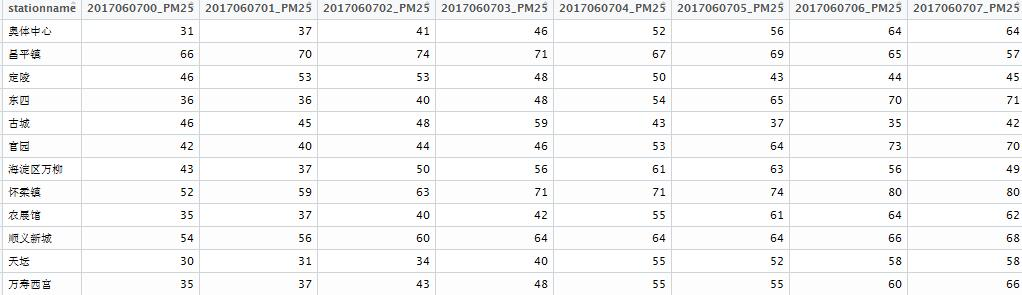
\includegraphics[width=1\linewidth,height=0.25\textheight]{fig/fig25}

\begin{Shaded}
\begin{Highlighting}[]
\NormalTok{dist.pm25<-}\KeywordTok{dist}\NormalTok{(airnew[,}\OperatorTok{-}\DecValTok{1}\NormalTok{],}\DataTypeTok{method=}\StringTok{'euclidean'}\NormalTok{)}
\KeywordTok{heatmap}\NormalTok{(}\KeywordTok{as.matrix}\NormalTok{(dist.pm25),}\DataTypeTok{labRow=}\NormalTok{stationname)}
\end{Highlighting}
\end{Shaded}

我们做的分析是对一天内24小时下12个站点的PM2.5聚类分析。所以这个问题的多元变量,是不同时间段的PM2.5值,前期已经把数据结构成功做成矩阵形式,接下来就需要计算距离了。距离矩阵在R里面是比较好求取的。dist函数。dist函数的参数事实上有不少,但是其实一般重点用的就是输入矩阵的参数(代码中的airnew{[},-1{]},-1代表去掉第一列数据(站点名称)),还有计算距离的方式------method。这里选的是欧氏距离。这个参数的可选取值还包括maximum(最大距离)、manhattan(曼哈顿距离)、canberra(兰氏威廉姆斯距离)、binary(定性距离,其实就是配合距离)、minkowski(闵可夫斯基距离------明氏距离)。还有用得多些的参数------diag和upper。diag为TRUE的时候给出对角线上的距离。upper为TURE的时候给出上三角矩阵上的值。默认都是FLASE。函数计算完之后得到的是一个距离矩阵。我们用热力图的方式进行可视化,这就是上面的第二句代码。heatmap函数是个热图可视化函数,要求输入一个矩阵。labRow其实是输入列名,labcol是与labRow相关,用来映射输入的值的。结果如下图。

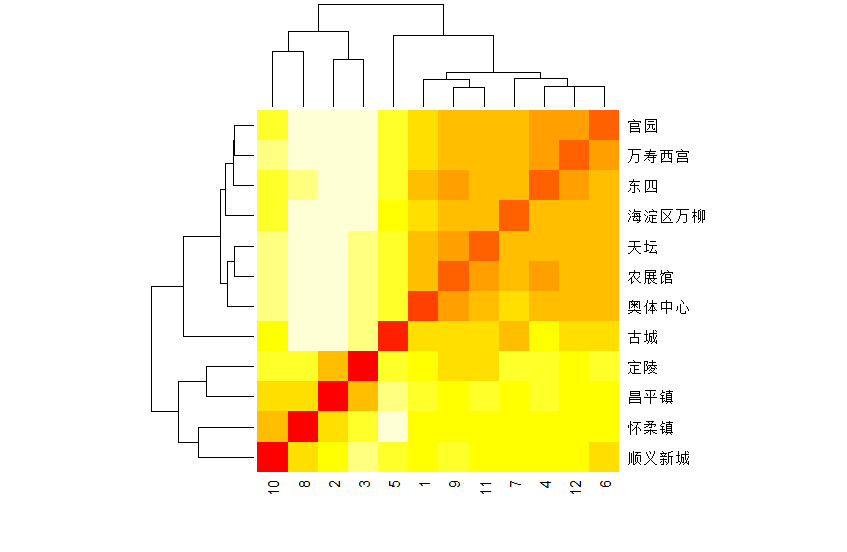
\includegraphics[width=1\linewidth,height=0.4\textheight]{fig/fig26}

计算完矩阵,即可进行聚类分析了。hclust函数的必要参数与前面距离的参数类似------输入矩阵参数,方法参数(这里聚类的方法前面也有提到,这里就不赘述了,有兴趣的可以自己看官方帮助文档)。而聚类完的结果存储在model1里面,用plot即可画出聚类谱系图。事实上,plclust也是相同的作用,参数基本是统一的,labels填写我们聚类的变量。而聚类完的结果则可以用cutree来获得,输入的model1------聚类结果,k是要求的类数。

\begin{Shaded}
\begin{Highlighting}[]
\NormalTok{model1 =}\StringTok{ }\KeywordTok{hclust}\NormalTok{(dist.pm25, }\DataTypeTok{method =} \StringTok{"ward.D"}\NormalTok{)}
\KeywordTok{plot}\NormalTok{(model1, }\DataTypeTok{labels =}\NormalTok{ stationname, }\DataTypeTok{hang =} \DecValTok{-1}\NormalTok{, }\DataTypeTok{las =} \DecValTok{1}\NormalTok{)}
\end{Highlighting}
\end{Shaded}

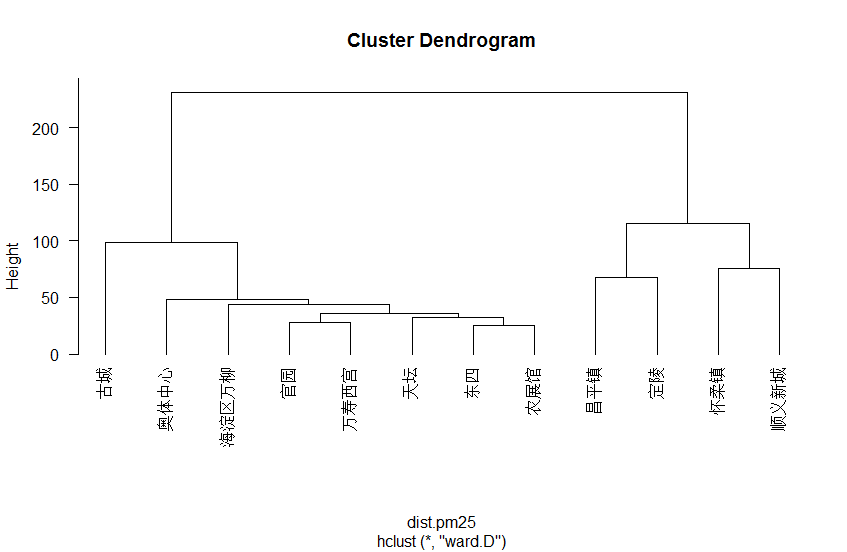
\includegraphics[width=1\linewidth,height=0.4\textheight]{fig/fig27}

对聚类结果做个简单可视化。以0点和1点的PM2.5值分别为x和y轴,以聚类结果做划分。

\begin{Shaded}
\begin{Highlighting}[]
\NormalTok{result =}\StringTok{ }\KeywordTok{cutree}\NormalTok{(model1, }\DataTypeTok{k =} \DecValTok{3}\NormalTok{)}
\KeywordTok{plot}\NormalTok{(airnew[, }\DecValTok{2}\NormalTok{], airnew[, }\DecValTok{3}\NormalTok{], }\DataTypeTok{col =}\NormalTok{ result, }\DataTypeTok{pch =} \KeywordTok{as.integer}\NormalTok{(result))}
\end{Highlighting}
\end{Shaded}

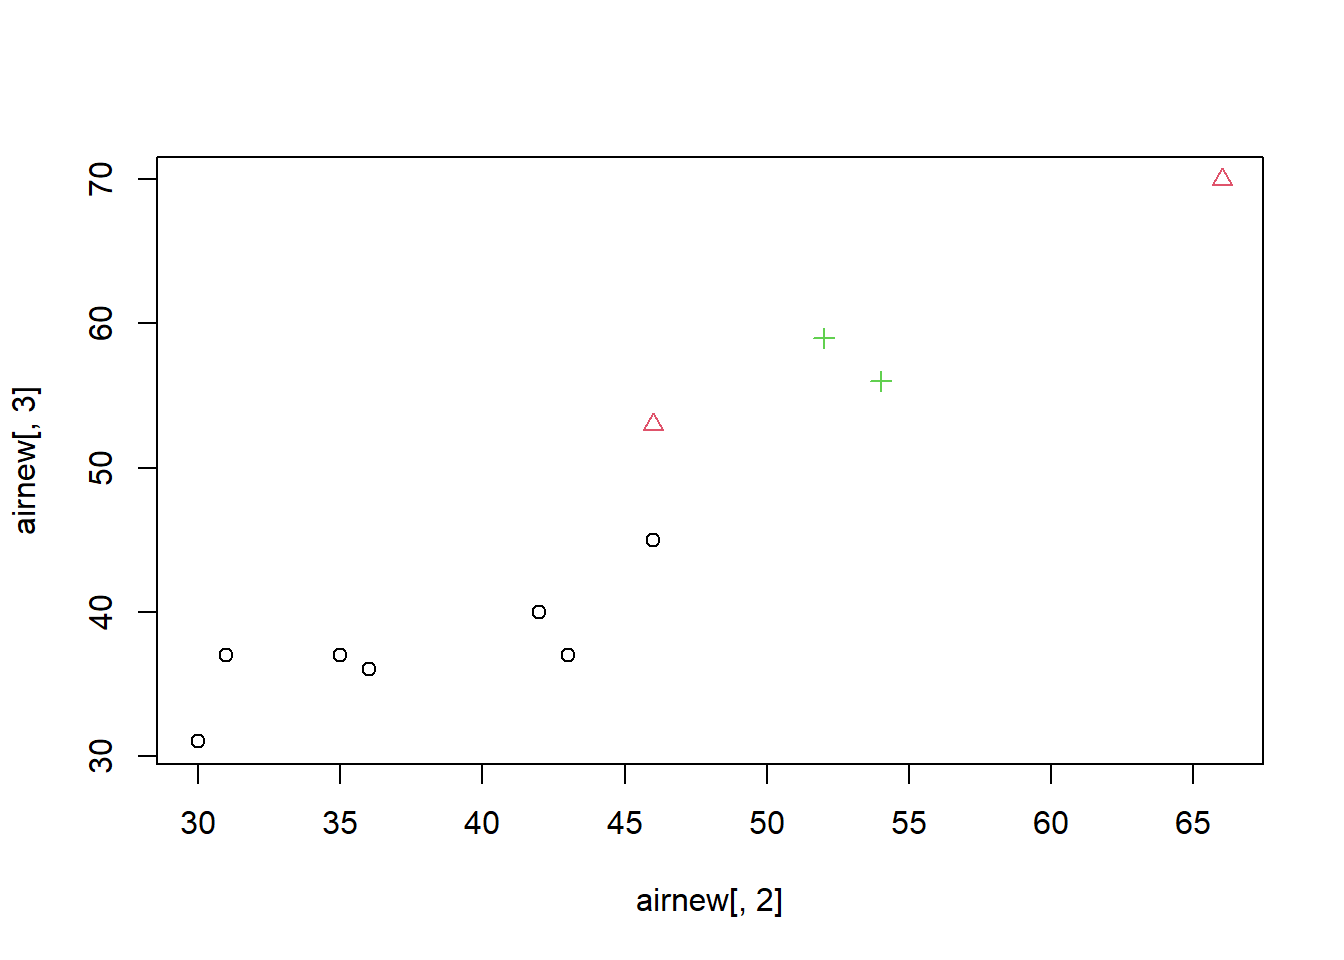
\includegraphics[width=1\linewidth,height=0.4\textheight]{bookdown_files/figure-latex/unnamed-chunk-63-1}

接下来是K-means的方法。函数并不复杂,输入数据框或者矩阵(做聚类的数据),center就是聚类数,nstart是迭代次数。迭代次数高,聚类可信度高些。后面的这个函数是聚类可视化的函数,是fpc包下面的,使用前请先确认是否安装。

\begin{Shaded}
\begin{Highlighting}[]
\NormalTok{kres <-}\StringTok{ }\KeywordTok{kmeans}\NormalTok{(airnew[, }\DecValTok{-1}\NormalTok{], }\DataTypeTok{centers =} \DecValTok{3}\NormalTok{, }\DataTypeTok{nstart =} \DecValTok{10}\NormalTok{)}
\KeywordTok{plotcluster}\NormalTok{(airnew[, }\DecValTok{-1}\NormalTok{], kres}\OperatorTok{$}\NormalTok{cluster)}
\end{Highlighting}
\end{Shaded}

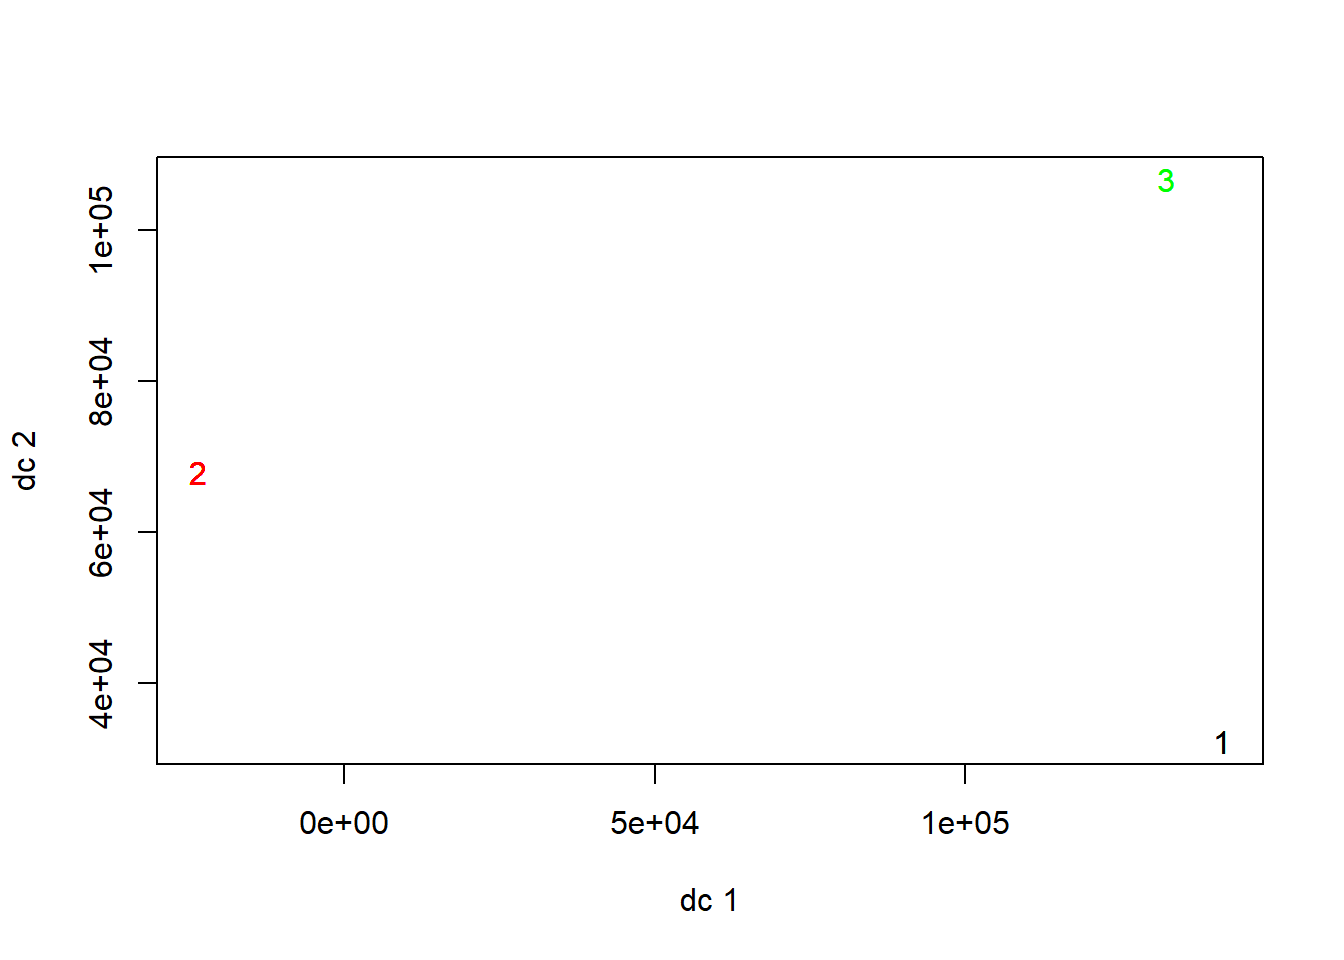
\includegraphics[width=1\linewidth,height=0.4\textheight]{bookdown_files/figure-latex/unnamed-chunk-65-1}

对比了二者的分类结果,是一致的。

\includegraphics[width=1\linewidth,height=0.4\textheight]{bookdown_files/figure-latex/unnamed-chunk-66-1}

聚类结束后,我们就这个数据和结果做些简单的分析。事实上作为地学人员,我们就简单地画个站点分布图来对应看看具体情况。从这张图来看,PM2.5的聚类结果显示了它具有很好的空间分异性。当然下面的图有点简陋,给出一个对比的,基于leaflet和R Notebook的交互式小地图(老规矩)。

\includegraphics[width=1\linewidth,height=0.3\textheight]{bookdown_files/figure-latex/unnamed-chunk-67-1}

\includegraphics[width=1\linewidth,height=0.6\textheight]{bookdown_files/figure-latex/unnamed-chunk-68-1}

\hypertarget{discriminant}{%
\chapter{Discriminant Analysis}\label{discriminant}}

本篇是第十一章,内容是判别分析。

\hypertarget{ux5224ux522bux5206ux6790ux5e94ux7528}{%
\section{判别分析应用}\label{ux5224ux522bux5206ux6790ux5e94ux7528}}

判别分析(Discriminant Analysis)------判别分析的目的是对已知分类的数据建立由数值指标构成的分类规则,然后把这样的规则应用到未知分类的样本中去分类,以识别未知样本所属的类别。判别分析是多元数据分析的重要方法之一。通常解决被解释变量是非数值变量,解释变量是数值变量的情形。

事实上地学领域应用判别分析最多的是在哪里呢?其实是遥感影像的地物分类,通常遥感导论中无论Erdas或者ENVI在做完监督分类之后,其实就是用标注的样本去训练判别函数,然后用判别函数完成整幅影像的判别分析,就可以分出不同的地物类型,这种方法就是我们最普遍使用的极大似然法。而这里的被解释变量就是地物类型,解释变量(多元)就是遥感影像不同波段的DN值,或者是辐射率。

\begin{quote}
\begin{itemize}
\tightlist
\item
  聚类分析和判别分析差异:在聚类分析中,人们一般事先并不知道应该分成几类及哪几类,全根据数据确定。在判别分析中,至少有一个已经明确知道类别的``训练样本'',并利用该样本来建立判别准则,并通过预测变量来为未知类别的观测值进行判别。通常实际问题中,可以先聚类以得知类型,再进行判别。
\end{itemize}
\end{quote}

\textbf{用机器学习的话来说,聚类分析是非监督学习,判别分析属于监督学习。}

判别分析的数据结构

\begin{longtable}[]{@{}lcccrr@{}}
\toprule
individuals & \(X_1\) & \(X_2\) & \(\cdots\) & \(X_l\) & \(\cdots\)\tabularnewline
\midrule
\endhead
1 & 28 & 1.0 & \(\cdots\) & 114 & \(\cdots\)\tabularnewline
2 & 29 & 2.0 & \(\cdots\) & 117 & \(\cdots\)\tabularnewline
\(\cdots\) & \(\cdots\) & \(\cdots\) & \(\cdots\) & \(\cdots\) & \(\cdots\)\tabularnewline
i & \(x_{i1}\) & \(x_{i2}\) & \(\cdots\) & \(x_{il}\) & \(\cdots\)\tabularnewline
\(\cdots\) & \(\cdots\) & \(\cdots\) & \(\cdots\) & \(\cdots\) & \(\cdots\)\tabularnewline
47 & 15 & 8 & \(\cdots\) & 64 & \(\cdots\)\tabularnewline
48 & 16 & 7.5 & \(\cdots\) & 65 & \(\cdots\)\tabularnewline
\(\cdots\) & \(\cdots\) & \(\cdots\) & \(\cdots\) & \(\cdots\) & \(\cdots\)\tabularnewline
n & \(x_{n1}\) & \(x_{n2}\) & \(\cdots\) & \(x_{nl}\) & \(\cdots\)\tabularnewline
\bottomrule
\end{longtable}

对比聚类分析的数据结构,事实上就是多了最后一列的Y。

\begin{quote}
\begin{itemize}
\tightlist
\item
  个体由\(X_1,X_2,\cdots,X_p\)变量描述。
\item
  有分类变量\(Y\)明确对个体分类。
\item
  问题:建立\(Y\)与\(X_1,X_2,\cdots,X_p\)变量间关系的函数。根据函数将新个体进行分类。
\end{itemize}
\end{quote}

\textbf{误判率}

误判率的高低有下面两个因素决定:

\begin{quote}
\begin{itemize}
\tightlist
\item
  主观因素:分界线的位置要正确。
\item
  客观因素:均值,方差------通过选择指标来控制:一般来说,维度高一点,可以使分辨率高一些,但在许多情况下,指标太多,不仅不能提高分辨率,还增加计算量(需要丰富的实际经验和试算);在做判别分析前,要做假设检验。在两个总体的均值有显著差异的情况下,再做判别分析。
\end{itemize}
\end{quote}

\textbf{判别分析的假设}

\begin{quote}
\begin{itemize}
\tightlist
\item
  每一个判别变量(解释变量)不能是其他判别变量的线性组合------不符合该假设的话,无法估计判别函数,变量间高度相关或一变量与其他变量的线性组合高度相关时,参数估计的标准误差将很大。
\item
  判别变量之间具有多元正态分布------可精确的计算显著性检验值和归属概率。
\item
  如要采用线性判别函数,还要求各组协方差距阵相等------线性判别函数使用起来最方便、在实际中使用最广。
\end{itemize}
\end{quote}

\hypertarget{ux5224ux522bux5206ux6790ux65b9ux6cd5}{%
\section{判别分析方法}\label{ux5224ux522bux5206ux6790ux65b9ux6cd5}}

\hypertarget{ux8dddux79bbux5224ux522bux6cd5}{%
\subsection{距离判别法}\label{ux8dddux79bbux5224ux522bux6cd5}}

\textbf{两总体情况}

假设有两个总体\(G_1\)和\(G_2\),如果能够定义点x到它们的距离d(x,\(G_1\))和d(x,\(G_2\)),则可用如下规则进行判别:

\begin{quote}
\begin{itemize}
\tightlist
\item
  如果d(x,\(G_1\)) \textless{} d(x,\(G_2\))则\(x\in G_1\)
\item
  如果d(x,\(G_2\)) \textless{} d(x,\(G_1\))则\(x\in G_2\)
\item
  如果d(x,\(G_1\)) = d(x,\(G_2\))则待判。
\end{itemize}
\end{quote}

距离常选用马氏距离------假设\(\mu_1,\mu_2,\Sigma_1,\Sigma_2\)分别为\(G_1\)和\(G_2\)的均值向量和协方差阵,则点\(x\)到\(G_i\)的马氏距离为

\[d^2(x,G_i)=(x-\mu_i)'(\Sigma_i)^{-1}(x-\mu_i)\]

马氏距离的好处是可以克服变量之间的相关性干扰,并且消除各变量量纲的影响。

\begin{quote}
\begin{itemize}
\tightlist
\item
  \[\Sigma_1=\Sigma_2=\Sigma\]
\end{itemize}
\end{quote}

\begin{itemize}
\tightlist
\item
  定义:
\end{itemize}

\[\begin{aligned}
d^2(x,G_1)-d^2(x,G_2) & =(x-\mu_1)'\Sigma^{-1}(x-\mu_1)-(x-\mu_2)'\Sigma^{-1}(x-\mu_2) \\ &=-2[x-(\mu_1+\mu_2)/2]'\Sigma^{-1}(\mu_1-\mu_2) \end{aligned}\]

令:\[\bar\mu=(\mu_1+\mu_2)/2, \alpha=\Sigma^{-1}(\mu_1-\mu_2),W(x)=(x-\bar\mu)'\alpha=\alpha'(x-\bar\mu)\]

判别规则:

\begin{quote}
\begin{itemize}
\tightlist
\item
  如果\(W(x)>0\cdot d(x\cdot G_1) < d(x\cdot G_2)\)则\(x\in G_1\)
\item
  如果\(W(x)<0\cdot d(x,G_,1) > d(x\cdot G_2)\)则\(x\in G_2\)
\item
  如果\(W(x)=0,d(x\cdot G_1) = d(x\cdot G_2)\)则待判。
\end{itemize}
\end{quote}

称W(x)为判别函数(discriminant function),α为判别系数。当\(\mu_1,\mu_2,\Sigma\)未知时,可通过样本来估计。\(x_1^{(i)},\cdots,x_{n_i}^{(i)}\)为来自\(G_i\)的样本(i=1,2)。

\[\hat\mu^{(i)}=\frac{1}{n_i}\sum_{k=1}^{n_2}x_k^{(i)}=\bar x^{(i)},\hat \Sigma=\frac{1}{n_1+n_2-2}(S_1+S_2)\]

\[S_i=\sum_{t=1}^{n_i}(x_t^{(i)}-\bar x^{(i)})(x_t^{(i)}-\bar x^{(i)})',\bar x=\frac{1}{2}(\bar x^{(1)}+\bar x^{(2)})\]

判别函数为\(W(x)=(x-\bar x)'\hat \Sigma^{-1}(\bar x^{(1)}-\bar x^{(2)})\)

\begin{quote}
\begin{itemize}
\tightlist
\item
  \[\Sigma_1 \neq \Sigma_2\]
\end{itemize}
\end{quote}

判别函数为二次函数

\[W(x)=d^2(x,G_2)-d^2(x,G_1)=(x-\mu_2)'\Sigma_2^{-1}(x-\mu_2)-(x-\mu_1)'\Sigma_2^{-1}(x-\mu_1)\]

按照距离最近原则,判别准则为:

\begin{quote}
\begin{itemize}
\tightlist
\item
  如果\(W(x)>0\cdot d(x\cdot G_1) < d(x\cdot G_2)\)则\(x\in G_1\)
\item
  如果\(W(x)<0\cdot d(x,G_,1) > d(x\cdot G_2)\)则\(x\in G_2\)
\item
  如果\(W(x)=0,d(x\cdot G_1) = d(x\cdot G_2)\)则待判。
\end{itemize}
\end{quote}

\textbf{多总体情况}

\begin{quote}
\begin{itemize}
\tightlist
\item
  多总体情况:协方差相同,假设有k个总体\(G_1,G_2,\cdots,G_k\),它们的均值向量分别为\(\mu_1,\mu_2,\cdots,\mu_k\),协方差阵为\(\Sigma\),类似于两总体的讨论,判别函数为:
\end{itemize}
\end{quote}

\[W_{ij}(x)=[x-(\mu_i+\mu_j)/2]'\Sigma^{-1}(\mu_i-\mu_j),i,j=1,\cdots,k\]

判别规则:

\begin{quote}
\begin{itemize}
\tightlist
\item
  如果存在i,对所有\(j\neq i\),有\(W_{ij}(x)>0\),则\(x\in G_i\),否则待判。
\item
  如果服从多元正态分布,且各组协方差相同
\end{itemize}
\end{quote}

\[\begin{aligned} d^2(x,G_i)& =(x-\mu_i)'\Sigma^{-1}(x-\mu_i) \\ & =x'\Sigma^{-1}x-2(x'\Sigma^{-1}\mu_i-\mu_i'\Sigma^{-1}\mu_i/2) \\ & =x'\Sigma^{-1}x-f_i(x)\end{aligned}\]

在所有的\(f_i(x)\)中,哪个\(f_i(x)\)的值大,x到相应的组i的马氏距离小,判\(x\in G_i\)

\begin{quote}
\begin{itemize}
\tightlist
\item
  多总体情况:协方差不等,假设有k个总体\(G_1,G_2,\cdots,G_k\),它们的均值向量分别为\(\mu_1,\mu_2,\cdots,\mu_k\),协方差阵为\(\Sigma_1,\Sigma_2,\cdots,\Sigma_k\),类似于两总体的讨论,判别函数为:
\end{itemize}
\end{quote}

\[W(x)=(x-\mu_j)'\Sigma_j^{-1}(x-\mu_j)-(x-\mu_i)'\Sigma_i^{-1}(x-\mu_i),i,j=1,\cdots,k\]

判别规则:

\begin{quote}
\begin{itemize}
\tightlist
\item
  如果存在i,对所有\(j\neq i\),有\(W_{ij}(x)>0\),则\(x\in G_i\),否则待判。
\item
  如果总体均值、协方差未知,用样本均值、协方差估计。
\item
  若总体不服从正态分布,直接从马氏距离来做判别分析,失去了概率意义,仅仅是一直观的经验判断而已,可能偏误较大。
\end{itemize}
\end{quote}

\hypertarget{fisherux5224ux522bux6cd5}{%
\subsection{Fisher判别法}\label{fisherux5224ux522bux6cd5}}

Fisher判别法的思想就是投影,将k组p维数据投影到某一个方向,使得它们的投影组与组之间尽可能的分开。考虑只有两个(预测)变量的判别问题。假定只有两类。数据中的每个观测值是二维空间的一个点。这里只有两种已知类型的训练样本。一 类 有 38 个 点 (用``o''表示),另一类有44个点(用``*''表示)。按原来变量(横坐标和纵坐标),很难将这两种点分开。

\includegraphics[width=0.8\linewidth,height=0.4\textheight]{fig/fig28}

但是沿着图上的虚线方向朝和这个虚线垂直的一条直线进行投影会使得这两类分得最清楚。可以看出,如果向其他方向投影,判别效果不会比这个好。有了投影之后,再用前面讲到的距离远近的方法得到判别准则。这种先投影的判别方法就是Fisher判别法。

Fisher判别法

\begin{quote}
\begin{itemize}
\tightlist
\item
  不要求总体分布类型;
\item
  工作原理就是对原数据系统进行坐标变换,寻求能够将总体尽可能分开的方向;
\item
  a为\(R^p\)中的任一向量,点x在以a为法方向的投影为a'x;
\item
  各组数据的投影为:
\end{itemize}
\end{quote}

\[G_i:a'x_1^{(i)}\cdots a'x_n^{(i)},i=1,2,\cdots,k\]
\textgreater{} * 这些数据正好组成一元方差分析的数据。

将\(G_m\)组中数据投影的均值记为\(a'\bar x^{(m)}\),有:\(a'\bar x^{(m)}=\frac{1}{n_m}\sum_{i=1}^{n_m}a'\bar x_i^{(m)} ,m=1,\cdots,k\),记k组数据投影的总均值为\(a'\bar x\),有:\(a'\bar x=\frac{1}{n}\sum_{m=1}^{k}\sum_{i=1}^{n_m}a'\bar x_i^{(m)}\)。

组间离差平方和为:

\[SSG=\sum_{m=1}^{k}n_m(a'\bar x^{(m)}-a'\bar x)^2=a'[\sum_{m=1}^{k}n_m(\bar x^{(m)}-\bar x)(\bar x^{(m)}-\bar x)']a=a'Ba;\]

\[B=\sum_{m=1}^{k}n_m[(\bar x^{(m)}-\bar x)(\bar x^{(m)}-\bar x)']\]

组内离差平方和为:

\[SSE=\sum_{m=1}^k \sum_{i=1}^{n_m}(a'\bar x^{(m)}-a'\bar x)^2=a'[\sum_{m=1}^k \sum_{i=1}^{n_m}(\bar x^{(m)}-\bar x)(\bar x^{(m)}-\bar x)']a=a'Ea\]

\[E=\sum_{m=1}^k \sum_{i=1}^{n_m}(\bar x^{(m)}-\bar x)(\bar x^{(m)}-\bar x)'\]

如果K组有显著差异,则

\[F=\frac{SSG/(k-1)}{SSE/(n-k)}=\frac{n-k}{k-1}\frac{a'Ba}{a'Ea}\]

F应充分大,即希望找到a使得SSG尽可能大而SSE尽可能小。

\[\Delta (a)=\frac{a'Ba}{a'Ea}\rightarrow max\]

使\(\frac{a'Ba}{a'Ea}\)最大的值为方程\(\left|B-\lambda E\right|=0\)的最大特征根\(\lambda_1\)。记方程\(\left|B-\lambda E\right|=0\)的全部特征根为\(\lambda_1\ge \cdots \ge \lambda_r>0\),相应的特征向量为\(v_1,\cdots,v_r\)。\(\Delta (a)\)的大小可以估计判别函数\(y_i (x)=v_i'x(=a'x)\)的效果。记\(p_i\)为判别能力(效率),有:

\[p_i=\frac{\lambda_i}{\sum_{h=1}^r \lambda_h}\]

在有些问题中,仅用一个线性判别函数不能很好区别各个总体,可取第二个、第三个,以此类推。 m个判别函数的判别能力定义为:

\[\sum_{i=1}^mp_i=\frac{\sum_{i=1}^m\lambda_i}{\sum_{h=1}^r \lambda_h}\]

据此来确定选择多少判别函数。

\textbf{判别准则}

选择i使得:\(v_1'(x-\mu_i)+\cdots+v_m'(x-\mu_i)\)的值最小。

\textbf{Fisher判别法实质}

\begin{quote}
\begin{itemize}
\tightlist
\item
  选几个新的综合性指标,代替原来的p个指标。
\item
  构成新的综合性指标的条件:
\end{itemize}
\end{quote}

\begin{quote}
(1)不同类的均值差距尽可能大;
(2)各类中的方差尽可能小。
\end{quote}

Fisher判别法的依据不是x属于哪个总体的概率的大小,而是类别之间具有最大的可分性,也没有考虑错判带来的损失大小(错报台风登陆vs.漏报台风登陆)。

\hypertarget{bayesux5224ux522bux6cd5}{%
\subsection{Bayes判别法}\label{bayesux5224ux522bux6cd5}}

\begin{quote}
\begin{itemize}
\tightlist
\item
  不用判别式,而是比较新给样品属于各个总体的条件概率p(g\textbar x),\(g=1,\cdots,k\)的大小,将新样品判归为来自条件概率最大的总体。
\item
  先给出 k 个总体的先验概率\(q_1,\cdots,q_k\)(实践中通常把频率作为先验概率)。如各总体密度为\({f_k(x)}\),则后验概率为(\(g=1,\cdots,k\)):\(P(g|x)=q_gf_g(x)/\Sigma_i q_if_i(x)\)。
\item
  当且仅当\(P(h|x)= max_gP(g|x)\),判x来自第h总体。
\item
  也可以用使错判的损失最小的准则来判别。
\item
  设(\(D_1,D_2,\cdots,D_K\))是\(R_p\)的一个完备的划分,当样品x属于\(D_i\),就判x来自\(G_i\)。
\item
  记\(p(j|i), c(j|i)\)分别为来自i总体的个体被错判到第j总体的概率和损失。定义平均错判损失(ECM: expected cost of misclassification)为\(ECM(D)=\Sigma_{i=1\cdots k}q_i[\Sigma_{j=1\cdots k}p(j|i)c(j|i)]\)
\item
  Bayes判别法就是要选择划分D使得ECM(D)最小。
\end{itemize}
\end{quote}

\hypertarget{ux5efaux7acbux5224ux522bux51fdux6570ux7684ux65b9ux6cd5}{%
\section{建立判别函数的方法}\label{ux5efaux7acbux5224ux522bux51fdux6570ux7684ux65b9ux6cd5}}

与多元回归类似,变量选择的好坏直接影响判别分析的效果。常遇问题:(1)忽略最主要的指标;(2)引入太多指标,计算量既大又干扰分析。

\begin{quote}
\begin{itemize}
\tightlist
\item
  全模型法(SPSS系统默认方法)
\item
  前向选择法:从没有变量的模型开始 每一部逐步把对判别函数贡献最大的变量加入模型,直到模型外没有一个变量符合条件为止。当希望有较多变量进入判别函数时,选用此方法(在Syntax中实现)。选择使威尔克斯统计量最小且显著的变量加入。
\item
  后向选择法:从包含用户指定的所有变量的模型开始。每一部逐步把对判别函数贡献最小的变量从模型中剔除出去,直到留在模型中的变量都符合条件为止。当希望判别函数含有较少变量时,选用此方法。选择使威尔克斯统计量最大且不显著的变量剔除。
\item
  逐步选择法:前向选择和后向选择的结合。从没有变量的模型开始。每一部逐步把对判别函数贡献最大的变量加入模型,同时,对模型中的变量进行检验,把不符合条件的变量从模型中删除。是一种较好的方法。选择使威尔克斯统计量最小且显著的变量加入。选择使威尔克斯统计量最大且不显著的变量剔除。
\end{itemize}
\end{quote}

\hypertarget{ux5224ux522bux5206ux6790ux7684ux6b65ux9aa4ux53caux6ce8ux610fux4e8bux9879}{%
\section{判别分析的步骤及注意事项}\label{ux5224ux522bux5206ux6790ux7684ux6b65ux9aa4ux53caux6ce8ux610fux4e8bux9879}}

\textbf{判别分析的步骤}

\begin{quote}
\begin{itemize}
\tightlist
\item
  第1步:确定研究的问题与目的:判别分析适合将个体归类的问题,特别适合一个定性的被解释变量和多个定量的解释变量的情形。
\item
  第2步:判别分析研究设计
  解释变量与被解释变量的选择:被解释变量的组数可以是两个或更多,但必须互斥和完备。
  样本容量:判别分析对样本量与预测变量的比率敏感。
  总样本量:建议比率为每个解释变量20个观测,最小的总样本量为每个变量5个观测。最小的组的大小必须超过解释变量的个数,建议每组至少有20个观测,还要注意组的相对大小(大的组有不相称的高的分类机会)。样本分割:需要将样本分割为两个子样本,一个用于估计判别函数,另一个用于验证。随机分组,最常见的是随机分为两半。通常各组比率相同。
\item
  第3步:判别分析的假定
  多元正态性,如不满足建议使用Logistic回归。Box's Test 检验各组协方差阵是否相等,不等的协方差矩阵可能会负面影响分类过程,观测会被``过度归类''到大的协方差阵组中。解释变量的多重共线性。
\item
  第4步:估计判别模型和评估整体拟和统计显著性:
  Wilks' Lambda, Hotelling迹和Pillai评估判别函数的判别效力的显著性。评估整体拟和:计算每个观测的判别Z得分,检验各组在判别Z得分上的差异,评估组,关系的预测精度。
\item
  第5步:结果的解释
  解释判别分析中每个解释变量的相对重要性。标准化判别权重(判别系数):如存在多重共线性时不合适,可能不稳定。判别载荷,又称结构相关系数,是每个解释变量与判别函数的简单相关系数,也可能不稳定。偏F值。能力指数:当保留多个判别函数时。
\item
  第6步:结果的验证
  分隔样本或交叉验证法。
\end{itemize}
\end{quote}

\textbf{判别分析注意事项}

\begin{quote}
\begin{itemize}
\tightlist
\item
  解释变量(判别变量)必须是可测量的。
\item
  每一个判别变量不能是其它判别变量的线性组合(不能提供新的信息,无法估计判别函数)。
\item
  判别变量不能高度相关,否则导致估计的标准误差很大。
\item
  训练样本中必须包含所有要判别的类型,分类必须清楚(在判别分析前最好应当做假设检验,确定各个类的有关变量的均值是显著不同的)。
\item
  要选择好可能用于判别的预测变量。判别分析是为了正确地分类,但同时也要注意使用尽可能少的预测变量来达到这个目的。使用较少的变量意味着节省资源和易于对结果作解释。
\item
  检验结果(在SPSS选项中选择Wilks' Lambda、Rao's V、 The Squared Mahalanobis Distance或The Sum of Unexplained Variations等检验的计算机输出),以确定是否分类结果仅由于随机因素。
\item
  对于多个判别函数,要弄清各自的重要性。
\item
  注意训练样本的正确和错误分类率。研究被误分类的观测值,看是否能找出原因。
\end{itemize}
\end{quote}

\hypertarget{rux8bedux8a00ux4e2dux5224ux522bux5206ux6790ux5b9eux73b0}{%
\section{R语言中判别分析实现}\label{rux8bedux8a00ux4e2dux5224ux522bux5206ux6790ux5b9eux73b0}}

正如上文提到的,我们以一个简单的地物分类的例子来进行实践。原始的遥感影像如图所示(高分一号卫星16 m数据)。

\includegraphics[width=1\linewidth,height=0.4\textheight]{bookdown_files/figure-latex/unnamed-chunk-70-1}

高分一号卫星有四个波段,分别显示如下:

\includegraphics[width=1\linewidth,height=0.5\textheight]{bookdown_files/figure-latex/unnamed-chunk-71-1}

我们随机在区域内生成了55个样本点,并根据目视解译做了分类,由于所处研究区位于新城且仅作测试,用地类型仅选择了两类:建设用地/不透水面和植被。前面已经用4,3,2显示了原始影像,红色部分即为植被。植被为类型1,建设用地/不透水面为类型2。

\includegraphics[width=1\linewidth,height=0.5\textheight]{fig/fig35}

另外我们随机在区域内还生成了10个样本点作为验证点。

\includegraphics[width=1\linewidth,height=0.5\textheight]{fig/fig36}

接着下来我们读取数据并且利用三种不同的判别分析方法进行判别分析地物类别。判别分析可以自己通过dist函数计算距离得到。现在已经有对应的包可以直接分析。这里推荐两个包(WMDB和MASS)。WMDB可以实现加权马氏距离判别分析和Bayes判别分析,MASS可以实现Fisher判别分析。

距离判别分析的函数为wmd。具体参数如下:

\begin{verbatim}
wmd(Trnx,TrnG,Tweight=NULL,Tstx=NULL,var.equal=F)
\end{verbatim}

Trnx是训练样本数据。TrnG为分类结果,Tweight为指定权重,可以根据主成分贡献计算或者取相等(原始的判别分析法),Tstx为待测样本数据,var.equal指定协方差矩阵是否相等。

Fisher判别分析的函数为lda。具体参数如下:

\begin{verbatim}
lda(formula,data,……,subset,na.action)
\end{verbatim}

formula形如groups\textasciitilde x1+x2+\ldots\ldots 的形式,data为数据集,subset指定训练样本,na.action指定有缺失值处理方式。

Bayes判别分析的函数为dbayes。具体参数如下:

\begin{verbatim}
dbayes(Trnx,TrnG,p=rep(1,length(levels(TrnG))),Tstx=NULL,var.equal=F)
\end{verbatim}

Trnx是训练样本数据。TrnG为分类结果,p为指定先验概率的向量,Tstx为待测样本数据,var.equal指定协方差矩阵是否相等。

接下来就是基于高分影像的四个波段进行训练和判别分析。

距离判别分析结果。

\includegraphics[width=1\linewidth,height=0.2\textheight]{fig/fig29}

Fisher判别分析结果。

\includegraphics[width=1\linewidth,height=0.3\textheight]{fig/fig30}

列联表分析及判别准确率。

\includegraphics[width=0.4\linewidth,height=0.1\textheight]{fig/fig31}

\includegraphics[width=0.6\linewidth,height=0.02\textheight]{fig/fig32}

Bayes判别分析结果。

\includegraphics[width=1\linewidth,height=0.2\textheight]{fig/fig33}

从样本数据来看,Fisher结果是最好的。接下来即按照训练好的判别规则进行分类。这里发现WMDB包的两个函数并没有提供预测功能,这里选用了另一个包klaR来做贝叶斯分类(朴素贝叶斯)。

分类结果对比:

\includegraphics[width=1\linewidth,height=0.4\textheight]{bookdown_files/figure-latex/unnamed-chunk-79-1}

为了验证准确率,这里利用随机生成的10个验证点进行精度验证。

\includegraphics[width=0.6\linewidth,height=0.2\textheight]{fig/fig34}

由于选取验证点较少,准确率都达到了100\%。从实际影像对比来看,似乎Bayes方法将更多细小的植被提取出来了,但是也有一部分道路错分。Fisher方法少提取了一部分,但错分的部分几乎没有。

\hypertarget{pca}{%
\chapter{Priciple Component Analysis}\label{pca}}

本篇是第十二章,内容是主成分分析。

\hypertarget{ux4e3bux6210ux5206ux5206ux6790ux57faux672cux601dux60f3}{%
\section{主成分分析基本思想}\label{ux4e3bux6210ux5206ux5206ux6790ux57faux672cux601dux60f3}}

依旧从问题开始本篇的介绍。地理学和生态学研究里经常遇到的问题就是,影响变量非常之多,而且地球表层地理生态环境现象无法使用控制变量的方式进行实验。同时影响变量非常多,经常出现变量冗余、冗杂的现象,同时多元分布数据本身对人类的认知就是一种挑战。这里举个栗子:比如在研究城市经济发展的时候,我们会考虑到的因素会包括第一产业、第二产业、第三产业占比,城市人口,城市地理位置,城市气候适宜度,政策扶持等等很多因子,但是这里有很多因子存在共线性的情况,也就是变量冗余冗杂。用矛盾论的话说,要抓住主要矛盾,那么如何在多元分布数据中分离出主要的因子,这就是本篇的主角主成分分析(Priciple Component Analysis,PCA)。

所以它的\textbf{基本思想}是,在社会经济的研究中,为了全面系统的分析和研究问题,必须考虑许多经济指标,这些指标能从不同的侧面反映我们所研究的对象的特征,但在某种程度上存在信息的重叠,具有一定的相关性。这种信息的重叠有时甚至会抹杀事物的真正特征与内在规律。

主成分分析是利用降维的思想, 在力求数据信息丢失最少的原则下,对高维的变量空间降维,即在众多变量中找出少数几个综合指标(原始变量的线性组合),并且这几个综合指标将尽可能多地保留原来指标变异方面的信息,且这些综合指标互不相关。这些综合指标就称为主成分。主成分的数目少于原始变量的数目。

在一个低维空间识辨系统要比在一个高维空间容易得多。因此,更容易抓住主要矛盾,揭示事物内部变量之间的规律性,使问题得到简化,提高分析效率。指标间具有相关性是做主成分分析的前提。

主成分分析是一种数学变换方法,它把给定的一组变量通过线性变换转换为一组不相关的变量。在这种变换中,保持变量的总方差不变,同时,使第一主成分具有最大方差,第二主成分具有次大方差,依此类推。

\textbf{主成分与原始变量间的关系}

(1)每一个主成分是原始变量的线性组合。

(2)主成分的数目少于原始变量的数目。

(3)主成分保留了原始变量的大多数变异信息。

(4)各主成分间互不相关。

\hypertarget{ux51e0ux4f55ux89e3ux91caux4e0eux6570ux5b66ux6a21ux578b}{%
\section{几何解释与数学模型}\label{ux51e0ux4f55ux89e3ux91caux4e0eux6570ux5b66ux6a21ux578b}}

\hypertarget{ux51e0ux4f55ux89e3ux91ca}{%
\subsection{几何解释}\label{ux51e0ux4f55ux89e3ux91ca}}

假定只有二维,即只有两个变量,由横坐标和纵坐标所代表;每个观测值都有相应于这两个坐标轴的坐标值。如果这些数据形成一个椭圆形状的点阵(这在二维正态的假定下是可能的)该椭圆有一个长轴和一个短轴。在短轴方向上数据变化较少。在极端的情况,短轴如退化成一点,长轴的方向可以完全解释这些点的变化,由二维到一维的降维就自然完成了。

\includegraphics[width=1\linewidth,height=0.5\textheight]{fig/pca}

由图可以看出这些样本点无论是沿着\(x_l\)轴方向或\(x_2\)轴方向都具有较大的离散性,其离散的程度可以分别用观测变量\(x_l\)的方差和\(x_2\)的方差定量地表示。显然,如果只考虑\(x_1\)和\(x_2\)中的任何一个,那么包含在原始数据中的经济信息将会有较大的损失。

当坐标轴和椭圆的长短轴平行,那么代表长轴的变量就描述了数据的主要变化,而代表短轴的变量就描述了数据的次要变化。但是,坐标轴通常并不和椭圆的长短轴平行。因此,需要寻找椭圆的长短轴,并进行变换,使得新变量和椭圆的长短轴平行。如果长轴变量代表了数据包含的大部分信息,就用该变量代替原先的两个变量(舍去次要的一维),降维就完成了。椭圆的长短轴相差得越大,降维也越有道理。

\hypertarget{ux6570ux5b66ux6a21ux578b}{%
\subsection{数学模型}\label{ux6570ux5b66ux6a21ux578b}}

如果我们将xl轴和x2轴先平移,再同时按逆时针方向旋转\(\theta\)角度,得到新坐标轴Fl和F2。Fl和F2是两个新变量。根据旋转变换的公式:

\[\begin{cases} y_1=x_1\cos\theta+x_2\sin\theta \\ y_2=-x_1\sin\theta+x_2\cos\theta \end{cases}\]

\[\begin{pmatrix} y_1 \\ y_2 \end{pmatrix}=\begin{pmatrix} \cos\theta & \sin\theta \\ -\sin\theta & \cos\theta \end{pmatrix} \begin{pmatrix} x_1 \\ x_2 \end{pmatrix}=U'x\]

\(U'\)为旋转变换矩阵,它是正交矩阵,即有\(U'=U^{-1},U'U^{-1}=I\)。旋转变换的目的是为了使得n个样品点在\(F_l\)轴方向上的离散程度最大,即\(F_l\)的方差最大。变量\(F_l\)代表了原始数据的绝大部分信息,在研究某经济问题时,即使不考虑变量\(F_2\)也无损大局。经过上述旋转变换原始数据的大部分信息集中到\(F_l\)轴上,对数据中包含的信息起到了浓缩作用。\(F_l\), \(F_2\)除了可以对包含在\(X_l\),\(X_2\)中的信息起着浓缩作用之外,还具有不相关的性质,这就使得在研究复杂的问题时避免了信息重叠所带来的虚假性。二维平面上的个点的方差大部分都归结在\(F_l\)轴上,而\(F_2\)轴上的方差很小。 \(F_l\)和\(F_2\)称为原始变量,\(x_1\)和\(x_2\)的综合变量。 简化了系统结构,抓住了主要矛盾。

\textbf{多维情形}

多维变量的情况和二维类似。正如二维椭圆有两个主轴,三维椭球有三个主轴一样,有几个变量,就有几个主轴。和二维情况类似,高维椭球的主轴也是互相垂直的。首先把高维椭球的主轴找出来,再用代表大多数数据信息的最长的几个轴作为新变量。这些互相正交的新变量是原先变量的线性组合,叫做主成分(principal component)。

假设我们所讨论的实际问题中,有p个指标,我们把这p个指标看作p个随机变量,记为\(X_1,X_2,\cdots,X_p\),主成分分析就是要把这个p指标的问题,转变为讨论p个指标的线性组合的问题,而这些新的指标\(F_1,F_2,\cdots,F_k(k\le p)\),按照保留主要信息量的原则充分反映原指标的信息,并且相互独立。

这种由讨论多个指标降为少数几个综合指标的过程在数学上就叫做降维。主成分分析通常的做法是,寻求原指标的线性组合Fi。
\[F_1=u_{11}X_1+u_{21}X_2+\cdots+u_{p1}X_p\]

\[F_2=u_{12}X_1+u_{22}X_2+\cdots+u_{p2}X_p\]

\[\cdots\]

\[F_p=u_{1p}X_1+u_{2p}X_2+\cdots+u_{pp}X_p\]

\textbf{满足条件}

每个主成分的系数平方和为1。即\(u_{1i}^2+u_{2i}^2+\cdots+u_{pi}^2=1\),主成分之间相互独立,即无重叠的信息。即\(Cov(F_i,F_j)=0,i\neq j,i,j=1,2,\cdots,p\)。主成分的方差依次递减,重要性依次递减,即\[Var(F_1)\ge Var(F_2)\ge \cdots \ge Var(F_p)\]

\hypertarget{ux4e3bux6210ux5206ux7684ux63a8ux5bfc}{%
\section{主成分的推导}\label{ux4e3bux6210ux5206ux7684ux63a8ux5bfc}}

\textbf{两个线性代数的结论}

(1)若A是p阶实对称矩阵,则一定可以找到正交阵U,使

\[U^{-1}AU=\begin{bmatrix} \lambda_1 & 0 & \cdots & 0 \\ 0 & \lambda_2 & \cdots & 0 \\ \vdots & \vdots & \ddots & \vdots \\ 0 & 0 & \cdots & \lambda_p \end{bmatrix}_{p\times p}\]

其中\(\lambda_i,i=1,2,\cdots,p\)是A的特征根。

(1)若上述矩阵的特征根所对应的单位特征向量为\(u_1,\cdots,u_p\)。令\(U=(u_1,\cdots,u_p)=\begin {bmatrix} u_{11} & u_{12} & \cdots & u_{1p} \\ u_{21} & u_{22} & \cdots & u_{2p} \\ \vdots & \vdots & & \vdots \\ u_{p1} & u_{p2} & \cdots & u_{pp} \end {bmatrix}\)则实对称阵A属于不同特征根所对应的特征向量是正交的,即有\(U'U=UU'=I\)

\textbf{第一主成分}

设X的协方差阵为\(\Sigma_x=\begin {bmatrix} \sigma_{11} & \sigma_{12} & \cdots & \sigma_{1p} \\ \sigma_{21} & \sigma_{22} & \cdots & \sigma_{2p} \\ \vdots & \vdots & & \vdots \\ \sigma_{p1} & \sigma_{p2} & \cdots & \sigma_{pp} \end {bmatrix}\)。由于\(\Sigma_x\)为非负定的对称阵,必存在正交阵U,使得:

\[U'\Sigma_x U=\begin {bmatrix} \lambda_1 & & 0 \\  & \ddots  & \\ 0 & & \lambda_p \end {bmatrix}\]

其中\(\lambda_1,\lambda_2,\cdots,\lambda_p\)为\(\Sigma_x\)的特征根。

不妨假设\(\lambda_1\ge \lambda_2\ge \cdots \ge \lambda_p\)。而U恰好是由特征根相对应的特征向量所组成的正交阵。

\[U=(u_1,\cdots,u_p)=\begin {bmatrix} u_{11} & u_{12} & \cdots & u_{1p} \\ u_{21} & u_{22} & \cdots & u_{2p} \\ \vdots & \vdots & & \vdots \\ u_{p1} & u_{p2} & \cdots & u_{pp} \end {bmatrix}\]

\[U_i=(u_{1i},u_{2i},\cdots,u_{pi})' i=1,2,\cdots,p\]

设有p维正交向量\(a_1=(a_{11},a_{21},\cdots,a_{p1})'\),\(F_1=a_{11}X_1+\cdots+a_{p1}X_p=a'X\),

\[V(F_1)=a_1'\Sigma a_1==a_1'U\begin {bmatrix} \lambda_1 & & & \\ & \lambda_2 & & \\ & & \cdots & & \\ & & & \lambda_p &\end {bmatrix}U'a_1\]

当且仅当\(a_1=u_1\)时,即\(F_1=u_{11}X_1+\cdots+u_{p1}X_p\)时,有最大的方差\(\lambda_1\)。\(Var(F_1)=U_1'\Sigma_x U_1=\lambda_1\)。如果第一主成分的信息不够,则需要寻找第二主成分。

\textbf{第二主成分}

在约束条件\(cov(F_1,F_2)=0\)下,寻找第二主成分,取线性变换,\(F_2=u_{12}X_1+\cdots+u_{p2}X_p\)的方差次大。

\[cov(F_1,F_2)=cov(u_1'x,u_2'x)=u_2'\Sigma u_1=\lambda_1 u_2'u_1=0\]

\[Var(F_2)=U_2'\Sigma_x U_2=\lambda_2\]

类推

\[F_1=u_{11}X_1+u_{21}X_2+\cdots+u_{p1}X_p\]

\[F_2=u_{12}X_1+u_{22}X_2+\cdots+u_{p2}X_p\]

\[\cdots\]

\[F_p=u_{1p}X_1+u_{2p}X_2+\cdots+u_{pp}X_p\]

写成矩阵形式:

\[F=U'X\]

\[U=(u_1,\cdots,u_p)=\begin {bmatrix} u_{11} & u_{12} & \cdots & u_{1p} \\ u_{21} & u_{22} & \cdots & u_{2p} \\ \vdots & \vdots & & \vdots \\ u_{p1} & u_{p2} & \cdots & u_{pp} \end {bmatrix}\]

\[X=(X_1,X_2,\cdots,X_p)'\]

\hypertarget{ux4e3bux6210ux5206ux7684ux6027ux8d28}{%
\section{主成分的性质}\label{ux4e3bux6210ux5206ux7684ux6027ux8d28}}

(1)\textbf{均值} \(E(U'x)=U'\mu\)

(2)\textbf{方差为所有特征根之和}

\[\sum_{i=1}^pVar(F_i)=\lambda_1+\lambda_2+\cdots+\lambda_p=\sigma_1^2+\sigma_2^2+\cdots+\sigma_p^2\]
说明主成分分析把p个随机变量的总方差分解成为p个不相关的随机变量的方差之和。协方差矩阵\(\Sigma\)的对角线上的元素之和等于特征根之和。

(3)\textbf{精度分析}

\begin{quote}
\begin{itemize}
\tightlist
\item
  贡献率:第i个主成分的方差在全部方差中所占比重\(\lambda_i/\sum_{i=1}^p\lambda_i\),称为贡献率,体现这个主成分的综合能力的大小,即反映原来p个指标的信息的多少。
\item
  累积贡献率:前k个主成分共有多大的综合能力,用这个k个主成分的方差和在全部方差中所占比重\(\sum_{i=1}^k\lambda_i/\sum_{i=1}^p\lambda_i\)来描述,称为累积贡献率。我们进行主成分分析的目的之一是希望用尽可能少的主成分\(F_1,F_2,\cdots,F_k(k\le p)\)代替原来的p个指标。到底应该选择多少个主成分,在实际工作中,所采用主成分个数的多少取决于能够反映原来变量85\%以上的信息量为依据,即当累积贡献率\(\geq85\)时\%的主成分的个数就足够了。最常见的情况是主成分为2到3个。
\end{itemize}
\end{quote}

(3)\textbf{载荷矩阵}

\[\begin {bmatrix} u_{11} & u_{12} & \cdots & u_{1m} \\ u_{21} & u_{22} & \cdots & u_{2m} \\ \vdots & \vdots & & \vdots \\ u_{p1} & u_{p2} & \cdots & u_{pm} \end {bmatrix}\]

\textbf{原始变量与主成分之间的相关系数}

\[F_j=u_{1j}x_1+u_{2j}x_2+\cdots+u_{pj}x_p j=1,2,\cdots,m,m\le p\]

\[F=U'X UF=X\]

\[\begin {bmatrix} x_1 \\ x_2 \\ \vdots \\ x_p \end {bmatrix}=\begin {bmatrix} u_{11} & u_{12} & \cdots & u_{1p} \\ u_{21} & u_{22} & \cdots & u_{2p} \\ \vdots & \vdots & & \vdots \\ u_{p1} & u_{p2} & \cdots & u_{pp} \end {bmatrix}\begin {bmatrix} F_1 \\ F_2 \\ \vdots \\ F_p \end {bmatrix}\]

\[Cov(x_i,F_j)=Cov(u_{i1}F_1+u_{i2}F_2+\cdots+u_{ip}F_p,F_j)=u_{ij}\lambda_j\]

\[\rho(x_i,F_j)=\frac{u_{ij}\lambda_j}{\sigma_i\sqrt{\lambda_j}}=\frac{u_{ij}\sqrt{\lambda_j}}{\sigma_i}\]

可见,\(x_i\)和\(F_j\)的相关的密切程度取决于对应线性组合系数的大小。该相关系数又叫因子负荷量。在解释主成分的成因或是第i个变量对第k个主成分的重要性时,应当根据因子负荷量而不是变换系数u.

\textbf{原始变量被主成分的提取率:}主成分的贡献率和累计贡献率度量了\(F_1,F_2,\cdots,F_m\)分别从原始变量\(X_1,X_2,\cdots,X_P\)中提取了多少信息。那么\(X_1,X_2, \cdots,X_P\)各有多少信息分别被\(F_1,F_2,\cdots,F_m\)提取?这可以用\(F_1,F_2,\cdots,F_m\)分别与\(X_1, X_2,\cdots,X_P\)的相关系数的平方来衡量。

\[Var(x_i)=Var(u_{i1}F_1+u_{i2}F_2+\cdots+u_{ip}F_p)\]

则

\[u_{i1}^2\lambda_1+u_{i2}^2\lambda_2+\cdots+u_{im}^2\lambda_m+\cdots+u_{ip}^2\lambda_p=\sigma_i^2\]

\(u_{ij}^2\lambda_j\)是\(F_j\)能说明的第i 原始变量的方差。\(u_{ij}^2\lambda_j/\sigma_i^2\)是\(F_j\)提取的第i原始变量信息的比重。
如果我们仅仅提出了m个主成分,则第i原始变量信息的被提取率为:

\[\Omega_i=\sum_{j=1}^m\lambda_ju_{ij}^2/\sigma_i^2=\sum_{j=1}^m\rho_{ij}^2\]

\textbf{公共成分}

定义:如果一个主成分仅仅对某一个原始变量有作用,则称为特殊成分。如果一个主成分对所有的原始变量都起作用,则称为公共成分。

\hypertarget{ux4e3bux6210ux5206ux5206ux6790ux7684ux6b65ux9aa4}{%
\section{主成分分析的步骤}\label{ux4e3bux6210ux5206ux5206ux6790ux7684ux6b65ux9aa4}}

第一步:由X的协方差阵或相关系数阵\(\Sigma\),求出其特征根,即解方程,可得特征根。

第二步:求出特征根所对应的特征向量\(U_1,U_2,\cdots,U_p\),

\[U_i=(u_{1i},u_{2i},\cdots,u_{pi})'\]

第三步:计算累积贡献率,给出恰当的主成分个数。

\[F_i=U_i'X,i=1,2,\cdots,k(k\le p)\]

第四步:计算所选出的k个主成分的得分。将原始数据的中心化值:

\[X_i^*=X_i-\bar X=(x_{1i}-\bar x_1,x_{2i}-\bar x_2,\cdots,x_{pi}-\bar x_p)'\]

代入前k个主成分的表达式,分别计算出各单位k个主成分的得分,并按得分值的大小排队。

\textbf{基于协方差矩阵}

在实际问题中, X的协方差通常是未知的,样品有

\[X_1=(x_{1l},x_{2l},\cdots,x_{pl})'(l=1,2,\cdots,n)\]

\[\hat \Sigma_x=(\frac{1}{n-1}\sum_{l=1}^n(x_{ij}-\bar x_i)(x_{jl}-\bar x_j))_{p\times p}\]

\textbf{基于相关系数矩阵}

如果变量有不同的量纲, 变量水平差异很大,应该基于相关系数矩阵进行主成分分析。不同的是计算得分时应采用标准化后的数据。

\hypertarget{ux4e3bux6210ux5206ux7684ux5e94ux7528ux4e0eux56deux5f52}{%
\section{主成分的应用与回归}\label{ux4e3bux6210ux5206ux7684ux5e94ux7528ux4e0eux56deux5f52}}

(1)主成分分析能降低所研究的数据空间的维数。即用研究m维的Y空间代替p维的X空间(\(m<p\)),而低维的Y空间代替高维的x空间所损失的信息很少。即使只有一个主成分\(Y_1\)(即m=1)时,这个\(Y_1\)仍是使用全部X变量(p个)得到的。在所选的前m个主成分中,如果某个\(X_i\)的系数全部近似于零的话,就可以把这个\(X_i\)删除,这也是一种删除多余变量的方法。

(2)多维数据的一种图形表示方法。多元统计研究的问题大都多于3个变量,要把研究的问题用图形表示出来是不可能的。然而,经过主成分分析后,我们可以选取前两个主成分或其中某两个主成分,根据主成分的得分,画出n个样品在二维平面上的分布情况,由图形可直观地看出各样品在主分量中的地位。

(3)用主成分分析法构造回归模型。即把各主成分作为新自变量代替原来的自变量做回归分析。

\textbf{主成分回归方法}

\[F_1=u_{11}X_1+u_{21}X_2+\cdots+u_{p1}X_p\]
\[F_2=u_{12}X_1+u_{22}X_2+\cdots+u_{p2}X_p\]

\[\cdots\]

\[F_p=u_{1p}X_1+u_{2p}X_2+\cdots+u_{pp}X_p\]

\[Y_i^*=\gamma_1F_{11}+\gamma_2F_{12}+\cdots+\gamma_mF_{1m}+\varepsilon_i\]

\[\sum_{i=1}^n[Y_i^*-\gamma_1F_{11}-\gamma_2F_{12}-\cdots-\gamma_mF_{1m}]^2=min\]

原始数据观测矩阵

\[X_0=\begin {bmatrix} x_{11} & x_{12} & \cdots & x_{1p} \\ x_{21} & x_{22} & \cdots & x_{2p} \\ \vdots & \vdots & & \vdots \\ x_{n1} & x_{n2} & \cdots & x_{np} \end {bmatrix}\]

主成分系数矩阵

\[U=(u_1,\cdots,u_p)=\begin {bmatrix} u_{11} & u_{12} & \cdots & u_{1p} \\ u_{21} & u_{22} & \cdots & u_{2p} \\ \vdots & \vdots & & \vdots \\ u_{p1} & u_{p2} & \cdots & u_{pp} \end {bmatrix}\]

主成分得分矩阵

\(\begin {bmatrix} F_{11} & F_{12} & \cdots & F_{1p} \\ F_{21} & F_{22} & \cdots & F_{2p} \\ \vdots & \vdots & & \vdots \\ F_{n1} & F_{n2} & \cdots & F_{np} \end {bmatrix}\)

\(F=X_0U\)

\textbf{主成分分析的一些注意事项}

主成分分析依赖于原始变量,也只能反映原始变量的信息。所以原始变量的选择很重要。
如果原始变量本质上独立,那么降维就可能失败,这是因为很难把很多独立变量用少数综合的变量概括。数据越相关,降维效果就越好。
分析结果并不一定会有清楚的解释。这与问题的性质,选取的原始变量以及数据的质量等都有关系。

\textbf{基于相关系数矩阵还是基于协方差矩阵做主成分分析?}

有时基于相关系数矩阵和基于协方差矩阵求出的主成分会有很大不同,且两者之间不存在简单的线性关系。
一般而言,当分析中所选择的经济变量具有不同的量纲,变量水平差异很大,应考虑将数据标准化,选择基于相关系数矩阵的主成分分析。对同度量或是取值范围在同量级的数据,选择基于协方差矩阵的主成分分析。

\textbf{选择几个主成分?}

主成分分析的目的是简化变量,一般情况下主成分的个数应该小于原始变量的个数。关于保留几个主成分,应该权衡主成分个数和保留的信息。

\textbf{如何解释主成分所包含的经济意义?}

主成分分析不要求数据来自于正态总体。一般认为当原始数据大部分变量的相关系数都小于0.3时,运用主成分分析的效果不显著。

\hypertarget{ux4e3bux6210ux5206ux5206ux6790ux7684rux8bedux8a00ux5b9eux73b0}{%
\section{主成分分析的R语言实现}\label{ux4e3bux6210ux5206ux5206ux6790ux7684rux8bedux8a00ux5b9eux73b0}}

主成分分析的函数本篇介绍的主要有两个。一个是princomp,一个是psych里的principal。

\begin{verbatim}
princomp(x,cor=FALSE,scores=TRUE)
\end{verbatim}

x为主成分分析数据集,cor=TRUE和FALSE分别代表是基于相关系数矩阵计算还是协方差矩阵计算。scores则代表是否存储主成分得分。

\begin{verbatim}
principal(x,nfactors=2,rotate="varimax",scores=T,covar=F)
\end{verbatim}

x为主成分分析数据集,nfactors为主成分个数,rotate表示旋转方式(一般选方差最大,保证互不相关),scores则代表是否存储主成分得分,covar=TRUE和FALSE分别代表是基于协方差矩阵计算还是相关系数矩阵计算。

这回用的数据是2006年城市统计年鉴285个地级市的经济人口数据,探究gdp与人口之间的关系。先做一个相关系数可视化。发现人口因子之间相互影响作用很高。

\includegraphics[width=1\linewidth,height=0.4\textheight]{bookdown_files/figure-latex/unnamed-chunk-82-1}

于是先对人口的几个因子进行降维和主成分分析,中途发现第三产业从业人数(third)加入会使得系数矩阵不正定,后面就删除了第三产业从业人数(third)。分别用不同方式进行主成分分析结果。

\begin{itemize}
\tightlist
\item
  princomp结果(基于协方差矩阵)
\end{itemize}

碎石图

\includegraphics[width=1\linewidth,height=0.4\textheight]{bookdown_files/figure-latex/unnamed-chunk-83-1}

结果

\includegraphics[width=1\linewidth,height=0.35\textheight]{fig/fig37}

主成分得分图

\includegraphics[width=1\linewidth,height=0.4\textheight]{bookdown_files/figure-latex/unnamed-chunk-85-1}

\begin{itemize}
\tightlist
\item
  princomp结果(基于相关系数矩阵)
\end{itemize}

碎石图

\includegraphics[width=1\linewidth,height=0.4\textheight]{bookdown_files/figure-latex/unnamed-chunk-86-1}

结果

\includegraphics[width=1\linewidth,height=0.35\textheight]{fig/fig38}

主成分得分图

\includegraphics[width=1\linewidth,height=0.4\textheight]{bookdown_files/figure-latex/unnamed-chunk-88-1}

\begin{itemize}
\tightlist
\item
  principal结果
\end{itemize}

碎石图

\includegraphics[width=1\linewidth,height=0.4\textheight]{bookdown_files/figure-latex/unnamed-chunk-89-1}

\begin{verbatim}
## Parallel analysis suggests that the number of factors =  NA  and the number of components =  2
\end{verbatim}

因子关系图

\includegraphics[width=1\linewidth,height=0.4\textheight]{bookdown_files/figure-latex/unnamed-chunk-90-1}

主成分得分图

\includegraphics[width=1\linewidth,height=0.4\textheight]{bookdown_files/figure-latex/unnamed-chunk-91-1}

碎石图表示的是曲线与纵坐标1交点的横坐标即为主成分个数,而主成分得分荷图是将原始数据的坐标映射在主成分分析的坐标上,事实上可以根据主成分得分在不同象限对原始数据进行分类,在本篇的样例数据里其实就是可以通过人口生成的几个主成分对中国地级市进行分类,可以区分出是在第一主成分得分高,第二主成分得分低的城市,亦或是其他排列组合的分类结果。关于这种可视化图具体如何解释。可以参照如下的文章。

\begin{quote}
\url{http://www.cnblogs.com/SCUJIN/p/5965946.html}
\end{quote}

\hypertarget{fa}{%
\chapter{Factor Analysis}\label{fa}}

本篇是第十三章,内容是因子分析。

\hypertarget{ux56e0ux5b50ux5206ux6790ux6982ux5ff5}{%
\section{因子分析概念}\label{ux56e0ux5b50ux5206ux6790ux6982ux5ff5}}

因子分析是一种数据简化的技术。它通过研究众多变量之间的内部依赖关系,探求观测数据中的基本结构,并用少数几个假想变量来表示其基本的数据结构。这几个假想变量能够反映原来众多变量的主要信息。原始的变量是可观测的显在变量,而假想变量是不可观测的潜在变量,称为因子。即一种用来在众多变量中辨别、分析和归结出变量间的相互关系并用简单的变量(因子)来描述这种关系的数据分析方法。

\textbf{寻求基本结构}

\begin{quote}
\begin{itemize}
\tightlist
\item
  通过因子分析,找出几个较少的有实际意义的因子,反映出原来数据的基本结构。
\item
  通常找出的这组观察不到的因子概括了原始的变量的大多数信息。
\end{itemize}
\end{quote}

\textbf{数据简化}

\begin{quote}
\begin{itemize}
\tightlist
\item
  强相关问题会对分析带来困难。
\item
  通过因子分析,可以用所找出的少数几个因子代替原来的变量做回归分析、聚类分析、判别分析等。
\end{itemize}
\end{quote}

\textbf{因子分析的用途}

\begin{quote}
\begin{itemize}
\tightlist
\item
  产生新的、更少的变量以便为后续的回归和其他分析做基础。
\item
  识别概念或产品的基本感知和特性。
\item
  改善市场研究领域多元测量的结构与方法。
\end{itemize}
\end{quote}

\hypertarget{ux56e0ux5b50ux5206ux6790ux6a21ux578b}{%
\section{因子分析模型}\label{ux56e0ux5b50ux5206ux6790ux6a21ux578b}}

\textbf{数学模型}:设\(X_i(i=1,2,\cdots,p)\)p个变量,如果表示为:

\[X_i=\mu_i+a_{i1}F_1+\cdots+a_{im}F_m+\varepsilon_i(m\le p)\]

或

\[\begin {bmatrix} X_1\\X_2\\\vdots\\X_p  \end {bmatrix}=\begin {bmatrix} \mu_1\\\mu_2\\\vdots\\\mu_p  \end {bmatrix}+\begin {bmatrix} \alpha_{11}&\alpha_{12}&\cdots&\alpha_{1m}\\\alpha_{21}&\alpha_{22}&\cdots&\alpha_{2m}\\\vdots&\vdots&&\vdots\\\alpha_{p1}&\alpha_{p2}&\cdots&\alpha_{pm} \end {bmatrix}\begin {bmatrix} F_1\\F_2\\\vdots\\F_m  \end {bmatrix}+\begin{bmatrix} \varepsilon_1\\ \varepsilon_2\\\vdots\\ \varepsilon_p  \end {bmatrix}\]

或

\[X-\mu=AF+\varepsilon\]

\(F_1,F_2,\cdots,F_m\)称为公共因子,是不可观测的变量,它们的系数称为因子载荷。\(\varepsilon_i\)是特殊因子,是不可能被前m个公共因子包含的部分。并且满足:\(cov(F,\varepsilon)=0\),即\(F,\varepsilon\)不相关;

\[D(F)=\begin {bmatrix} 1 & & & \\&1&&&\\&&\ddots&\\&&&1 \end {bmatrix}=I\]

即\(F_1,F_2,\cdots,F_m\)互不相关,方差为1。

\[D(\varepsilon)=\begin {bmatrix}\sigma_1^2&&&\\&\sigma_w^2&&&\\&&\ddots&\\&&&\sigma_p^2\end {bmatrix}\]

即\(\varepsilon_i\sim N(0,\sigma_i^2)\)互不相关,方差不一定相等。

\textbf{用矩阵的方式表达}

\[X-\mu=AF+\varepsilon\]

\[E(F)=0\]

\[E(\varepsilon)=0\]

\[Var(F)=1\]

\[cov(F,\varepsilon)=E(F\varepsilon')=\begin {pmatrix}E(F_1\varepsilon_1)&E(F_1\varepsilon_2)&\cdots&E(F_1\varepsilon_p)\\E(F_2\varepsilon_1)&E(F_2\varepsilon_2)&\cdots&E(F_2\varepsilon_p)\\\vdots&\vdots&&\vdots\\E(F_p\varepsilon_1)&E(F_p\varepsilon_2)&\cdots&E(F_p\varepsilon_p) \end {pmatrix}=0\]

\[Var(\varepsilon)=diag(\sigma_1^2,\sigma_2^2,\cdots,\sigma_p^2)\]

\textbf{因子分析模型的性质}

(1)原始变量X的协方差矩阵的分解

\[\Sigma_x=AA'+D\]

A是因子模型的系数

\[Var(\varepsilon)=D=diag(\sigma_1^2,\sigma_2^2,\cdots,\sigma_p^2)\]

D的主对角线上的元素值越小,则公共因子共享的成分越多。

(2)模型不受计量单位的影响。

(3)因子载荷不是惟一的:设T为一个p×p的正交矩阵,令\(A^*=AT, F^*=T'F\)也是一个满足因子模型条件的因子载荷。

\textbf{因子载荷矩阵中的统计特征}

\begin{quote}
\begin{itemize}
\tightlist
\item
  因子载荷\(a_{ij}\)是第i个变量与第j个公共因子的相关系数。
\item
  变量\(X_i\)的共同度是因子载荷矩阵的第i行的元素的平方和。记为\(h_i^2=\sum_{i=1}^ma_{ij}^2\)所有的公共因子和特殊因子对变量\(X_i\)的贡献为1。如果\(\sum_{i=1}^ma_{ij}^2\)非常靠近1, \(\sigma_i^2\)非常小,则因子分析的效果好,从原变量空间到公共因子空间的转化性质好。
\item
  因子载荷矩阵中各列元素的平方和\(S_j=\sum_{i=1}^pa_{ij}^2\)\(称为\)\(F_j(j=1,2,\cdots,m)\)对所有的\(X_i\)的方差贡献和。衡量\(F_j\)的相对重要性。
\end{itemize}
\end{quote}

\hypertarget{ux56e0ux5b50ux8f7dux8377ux77e9ux9635ux7684ux4f30ux8ba1ux65b9ux6cd5}{%
\section{因子载荷矩阵的估计方法}\label{ux56e0ux5b50ux8f7dux8377ux77e9ux9635ux7684ux4f30ux8ba1ux65b9ux6cd5}}

\begin{quote}
\begin{itemize}
\tightlist
\item
  主成分分析法:设随机向量\(x=(x_1,x_2,\cdots,x_p)'\)的均值为\(\mu\),协方差为\(\Sigma\),\(\lambda_1\ge\lambda_2\ge\cdots\ge\lambda_p\ge0\)为\(\Sigma\)的特征根,\(u_1,u_2,\cdots,u_p\)为对应的标准化特征向量,则:
\end{itemize}
\end{quote}

\[\Sigma=U\begin {bmatrix}\lambda_1&&&\\&\lambda_2&&\\&&\cdots&\\&&&\lambda_p \end {bmatrix}U'=AA'+D=\begin {bmatrix}\sqrt\lambda_1u_1&\sqrt\lambda_2u_2&\cdots&\sqrt\lambda_pu_p \end {bmatrix}\begin {bmatrix}\sqrt\lambda_1u_1'\\\sqrt\lambda_2u_2'\\\vdots\\\sqrt\lambda_pu_p' \end {bmatrix}+D\]

上式给出的\(\Sigma\)表达式是精确的,然而,它实际上是毫无价值的,因为我们的目的是寻求用少数几个公共因子解释,故略去后面的p-m项的贡献。上式有一个假定:模型中的特殊因子是不重要的,因而从的\(\Sigma\)的分解中忽略了特殊因子的方差。确定因子个数(特征根大于1所对应的特征向量;碎石原则:把特征根从大到小排列,把特征根减小速度变缓的特征根都删掉)。

\begin{quote}
\begin{itemize}
\tightlist
\item
  主因子法:主因子方法是对主成分方法的修正,假定我们首先对变量进行标准化变换。则\(R=AA'+D\)\$ \$\(^{\ast}=AA'=R-D\),称\(R^{\ast}\)为约相关矩阵,\(R^{\ast}\)对角线上的元素是\(h_i^2\),而不是1。
\end{itemize}
\end{quote}

\[R^{\ast}=R-\hat D=\begin {bmatrix}\hat h_1^2&r_{12}&\cdots&r_{1p}\\r_{21}&\hat h_2^2&\cdots&r_{2p}\\\vdots&\vdots&&\vdots\\r_{p1}&r_{p2}&\cdots&\hat h_p^2 \end {bmatrix}\]

直接求\(R^{\ast}\)的前p个特征根和对应的正交特征向量。得如下的矩阵:

\[A=\begin {bmatrix}\sqrt{\lambda_1^{\ast}}u_1^{\ast}&\sqrt{\lambda_2^{\ast}}u_2^{\ast}&\cdots&\sqrt{\lambda_p^{\ast}}u_p^{\ast} \end {bmatrix}\]

\(R^{\ast}\)特征根:\(\lambda_1^{\ast}\ge\lambda_2^{\ast}\ge\cdots\ge\lambda_p^{\ast}\ge0\),正交特征向量:\(u_1^{\ast},u_2^{\ast},\cdots,u_p^{\ast}\)。

当特殊因子\(\varepsilon_i\)的方差已知:

\[R^{\ast}=R-\begin {bmatrix}\sigma_1^2&&&\\&\sigma_2^2&&\\&&\ddots&\\&&&\sigma_p^2 \end {bmatrix}=\begin {bmatrix}\sqrt{\lambda_1^{\ast}}u_1^{\ast}&\sqrt{\lambda_2^{\ast}}u_2^{\ast}&\cdots&\sqrt{\lambda_p^{\ast}}u_p^{\ast} \end {bmatrix}\begin {bmatrix}\sqrt{\lambda_1^{\ast}}u_1^{'\ast}\\\sqrt{\lambda_2^{\ast}}u_2^{'\ast}\\\vdots\\\sqrt{\lambda_p^{\ast}}u_p^{'\ast} \end {bmatrix}\]

\[A=\begin {bmatrix}\sqrt{\lambda_1^{\ast}}u_1^{\ast}&\sqrt{\lambda_2^{\ast}}u_2^{\ast}&\cdots&\sqrt{\lambda_m^{\ast}}u_m^{\ast}\end {bmatrix}\]

\[D=\begin {pmatrix}1-\hat h_1^2&&0\\&\ddots&\\0&&1-\hat h_p^2 \end {pmatrix}\]

在实际的应用中,个性方差矩阵一般都是未知的,可以通过一组样本来估计。估计的方法有如下几种:

首先,求\(h_i^2\)的初始估计值,构造出\(R^*\)。

(1)取\(h_i^2=1\),在这个情况下主因子解与主成分解等价;

(2)取\(h_i^2=R_i^2\),\(R_i^2\)为\(x_i\)与其他所有的原始变量\(x_j\)的复相关系数的平方,即\(x_i\)对其余的p-1个\(x_j\)的回归方程的判定系数,这是因为xi与公共因子的关系是通过其余的p-1个\(x_j\)的线性组合联系起来的;

(3)取\(\hat h_i^2=max\left|r_{ij}\right|(j\neq i)\),这意味着取\(x_i\)与其余的\(x_j\)的简单相关系数的绝对值最大者;

(4)取\(h_i^2=\frac{1}{p-1}\sum_{j=1,j\neq i}^pr_{ij}\),其中要求该值为正数。

(5)取\(h_i^2=1/r^{ii}\),其中\(r^{ii}\)是\(R^{-1}\)的对角元。

(6) 极大似然估计法:如果假定公共因子F和特殊因子\(\varepsilon\)服从正态分布,那么可以得到因子载荷和特殊因子方差的极大似然估计。设\(x_1,x_2,\cdots,x_n\)为来自正态总体\(N_p(\mu,\Sigma)\)的随机样本。

\[\Sigma=AA'+\Sigma_{\varepsilon}\]

\[\begin {aligned} L(\hat \mu,\hat A,\hat D)&=f(X)=f(X_1)\cdot f(X_2)\cdots f(X_n)\\&=\prod_{i=1}^n(2\pi)^{-p/2}\left |\Sigma\right|^{1/2}exp\begin {bmatrix}-\frac{1}{2}(x_i-\mu)'\Sigma^{-1}(x_i-\mu) \end {bmatrix}\\&=\begin {bmatrix}(2\pi)^p\left |\Sigma \right |^{-n/2} \end {bmatrix}exp\begin {bmatrix}-\frac{1}{2}\sum_{i=1}^n(X_i-\mu)'\Sigma^{-1}(X_i-\mu) \end {bmatrix} \end {aligned}\]

用数值极大化的方法可以得到极大似然估计。

\hypertarget{ux56e0ux5b50ux65cbux8f6cux6b63ux4ea4ux53d8ux6362}{%
\section{因子旋转(正交变换)}\label{ux56e0ux5b50ux65cbux8f6cux6b63ux4ea4ux53d8ux6362}}

\textbf{旋转因子的目的:}因子分析的目的不仅仅是要找出公共因子以及对变量进行分组,更重要的是要知道每个公共因子的意义,以便进行进一步的分析。如果每个公共因子的含义不清,则不便于进行实际背景的解释。初始因子的综合性太强,难以找出因子的实际意义。由于因子载荷阵是不唯一的,所以可以对因子载荷阵进行旋转,使因子载荷阵的结构简化,使其每列或行的元素平方值向0和1两极分化。

\textbf{旋转方法:}设\(\Gamma\)正交矩阵,做正交变换\(B=A\Gamma\)。

\begin{quote}
\begin{itemize}
\tightlist
\item
  变换后各变量的共同度不会发生变化。
\item
  变换后各因子的贡献会发生变化。
\end{itemize}
\end{quote}

三种主要的正交旋转法。

\begin{quote}
\begin{itemize}
\tightlist
\item
  方差最大法L:方差最大法从简化因子载荷矩阵的每一列出发,使和每个因子有关的载荷的平方的方差最大。当只有少数几个变量在某个因子上有较高的载荷时,对因子的解释最简单。方差最大的直观意义是希望通过因子旋转后,使每个因子上的载荷尽量拉开距离,一部分的载荷趋于\(\pm1\),另一部分趋于0。
\end{itemize}
\end{quote}

\[A=\begin {bmatrix}a_{11}&a_{12}\\a_{21}&a_{22}\\\vdots&\vdots\\a_{p1}&a_{p2} \end {bmatrix}\]

\[X_1=a_{11}F_1+a_{12}F_2\]\[X_2=a_{21}F_1+a_{22}F_2\]\[\cdots\]\[X_p=a_{p1}F_1+a_{p2}F_2\]

设旋转矩阵:\(T=\begin {pmatrix}\cos\varphi&-\sin\varphi\\\sin\varphi&\cos\varphi \end {pmatrix}\),则

\[\begin {aligned}B&=AT=A\begin {pmatrix}\cos\varphi&-\sin\varphi\\\sin\varphi&\cos\varphi \end {pmatrix}\\&=\begin {pmatrix}a_{11}\cos\varphi+a_{12}\sin\varphi&-a_{11}\sin\varphi+a_{12}\cos\varphi\\\vdots&\vdots\\a_{p1}\cos\varphi+a_{p2}\sin\varphi&-a_{p1}\sin\varphi+a_{p2}\cos\varphi \end {pmatrix}\\&=\begin {pmatrix}a_{11}^{\ast}&a_{12}^{\ast}\\\vdots&\vdots\\a_{p1}^{\ast}&a_{p2}^{\ast} \end {pmatrix} \end {aligned}\]

令\(d_{ij}=\frac{a_{ij}^{\ast}}{h_i},i=1,2,\cdots,p;j=1,2\),\(\bar d_j=\frac{1}{p}\sum_{i=1}^pd_{ij}^2\)(这是列和),简化准则为:\(V(\theta)=\sum_{j=1}^m\sum_{i=1}^p(d_{ij}^2-\bar d_j)^2=max\),即:\(V_1+V_2+V_3+\cdots+V_m=max\)。

令\(\frac{\partial V}{\partial \theta}=0\),则可以解出\(\theta_0\),旋转矩阵为:\(T=\begin {pmatrix}\cos\theta_0&-\sin\theta_0\\\sin\theta_0&\cos\theta_0 \end {pmatrix}\)

\begin{quote}
\begin{itemize}
\tightlist
\item
  四次方最大法:四次方最大旋转是从简化载荷矩阵的行出发,通过旋转初始因子,使每个变量只在一个因子上有较高的载荷,而在其它的因子上尽可能低的载荷。 如果每个变量只在一个因子上有非零的载荷,这时的因子解释是最简单的。四次方最大法通过使因子载荷矩阵中每一行的因子载荷平方的方差达到最大。简化准则为:\(Q=\sum_{i=1}^p\sum_{j=1}^m(b_{ij}^2-\frac{1}{m})^2=max\)
\end{itemize}
\end{quote}

\[\begin {aligned} Q&=\sum_{i=1}^p\sum_{j=1}^m(b_{ij}^2-\frac{1}{m})^2=\sum_{i=1}^p\sum_{j=1}^m(b_{ij}^4-2\frac{1}{m}b_{ij}^2+\frac{1}{m^2})\\&=\sum_{i=1}^p\sum_{j=1}^m(b_{ij}^4-2\sum_{i=1}^p\sum_{j=1}^m\frac{1}{m}b_{ij}^2+\sum_{i=1}^p\sum_{j=1}^m\frac{1}{m^2})\\&=\sum_{i=1}^p\sum_{j=1}^m(b_{ij}^4-2\sum_{i=1}^p\sum_{j=1}^m\frac{1}{m}b_{ij}^2+\sum_{i=1}^p\sum_{j=1}^m\frac{1}{m^2})\\&=\sum_{i=1}^p\sum_{j=1}^m(b_{ij}^4-2+\frac{p}{m}) \end {aligned}\]

最终的简化准则为:\(Q=\sum_{i=1}^p\sum_{j=1}^mb_{ij}^4=MAX\)

\begin{quote}
\begin{itemize}
\tightlist
\item
  等量最大法:等量最大法把四次方最大法和方差最大法结合起来求Q和V的加权平均最大。最终的简化准则为:\(E=\sum_{i=1}^p\sum_{j=1}^mb_{ij}^4-\gamma\sum_{j=1}^m(\sum_{i=1}^pb_{ij}^2)^2/p=MAX\),权数\(\gamma\)等于\(m/2\),因子数有关。
\end{itemize}
\end{quote}

\hypertarget{ux56e0ux5b50ux5f97ux5206}{%
\section{因子得分}\label{ux56e0ux5b50ux5f97ux5206}}

当解决了用一组公共因子的线性组合来表示一组观测变量后,有时我们需要使用这些因子做其他的研究。比如把得到的因子作为自变量来做回归分析,对样本进行分类或评价,这就需要我们对公共因子进行测度,即给出公共因子的值。

\textbf{因子得分}

因子分析的数学模型:

\[\begin {bmatrix}X_1\\X_2\\\vdots\\X_p \end {bmatrix}=\begin {bmatrix}\alpha_{11}&\alpha_{12}&\cdots&\alpha_{1m}\\\alpha_{21}&\alpha_{22}&\cdots&\alpha_{2m}\\\vdots&\vdots&&\vdots\\\alpha_{p1}&\alpha_{p2}&\cdots&\alpha_{pm} \end {bmatrix}\begin {bmatrix}F_1\\F_2\\\vdots\\F_p \end {bmatrix}\]

原变量被表示为公共因子的线性组合,当载荷矩阵旋转之后,公共因子可以做出解释,通常的情况下,我们还想反过来把公共因子表示为原变量的线性组合。因子得分函数:\(F_j=\beta_{j1}X_1+\cdots+\beta_{jp}X_p, j=1,\cdots,m\)。可见,要求得每个因子的得分,必须求得分函数的系数,而由于p\textgreater m,所以不能得到精确的得分,只能通过估计。

\textbf{巴特莱特因子得分(加权最小二乘法)}

把\(x_i-\mu_i\)看作因变量;把因子载荷矩阵\(\begin {bmatrix}\alpha_{11}&\alpha_{12}&\cdots&\alpha_{1m}\\\alpha_{21}&\alpha_{22}&\cdots&\alpha_{2m}\\\vdots&\vdots&&\vdots\\\alpha_{p1}&\alpha_{p2}&\cdots&\alpha_{pm} \end {bmatrix}\)看成自变量的观测;把某个个案的得分\(F_j\)看作最小二乘法需要求的系数。

\[\begin {cases}x_{i1}-\mu_1=a_{11}f_1+a_{12}f_2+\cdots+a_{1m}f_m+\varepsilon_1\\x_{i2}-\mu_2=a_{21}f_1+a_{22}f_2+\cdots+a_{2m}f_m+\varepsilon_2\\\cdots\\x_{ip}-\mu_p=a_{p1}f_1+a_{p2}f_2+\cdots+a_{pm}f_m+\varepsilon_p \end {cases}\]

由于特殊因子的方差相异,所以用加权最小二乘法求得分,每个个案作一次,要求出所有样品的得分,需要作n次。

\[\sum_{j=1}^p[(x_i-\mu_i)-(a_{i1}\hat f_1+a_{i2}\hat f_2+\cdots+a_{im}\hat f_m)]^2/\sigma_i^2\]

使上式最小的\(\hat f_1,\cdots,\hat f_m\)是相应个案的因子得分。

\textbf{回归方法}

\[\begin {bmatrix}X_1\\X_2\\\vdots\\X_n \end {bmatrix}=\begin {bmatrix}\alpha_{11}&\alpha_{12}&\cdots&\alpha_{1m}\\\alpha_{21}&\alpha_{22}&\cdots&\alpha_{2m}\\\vdots&\vdots&&\vdots\\\alpha_{p1}&\alpha_{p2}&\cdots&\alpha_{pm} \end {bmatrix}\begin {bmatrix}F_1\\F_2\\\vdots\\F_p \end {bmatrix}+\begin {bmatrix}\varepsilon_1\\\varepsilon_2\\\vdots\\\varepsilon_n \end {bmatrix}\]

\[\hat F_j=b_{j1}X_1+\cdots+b_{jp}X_p, j=1,\cdots,m\]

\[\begin {bmatrix}b_{11}&b_{12}&\cdots&b_{1p}\\b_{21}&b_{22}&\cdots&b_{2p}\\\vdots&\vdots&&\vdots\\b_{m1}&b_{m2}&\cdots&b_{mp} \end {bmatrix}=\begin {bmatrix}b_1\\b_2\\\vdots\\b_m \end {bmatrix}\]

\[\begin {aligned} \alpha_{ij}=\gamma_{x_iF_j}=E(X_i,F_j)&=E[X_i(b_{j1}X_1+\cdots+b_{jp}X_p)]\\&=b_{j1}\gamma_{i1}+\cdots+b_{jp}\gamma_{ip}=\begin {bmatrix}\gamma_{i1}&\gamma_{i2}&\cdots&\gamma_{ip} \end {bmatrix}\begin {bmatrix}b_{j1}\\b_{j2}\\\vdots\\b_{jp} \end {bmatrix} \end {aligned}\]

则,我们有如下的方程组:

\[\begin {bmatrix}\gamma_{11}&\gamma_{12}&\cdots&\gamma_{1p}\\\gamma_{21}&\gamma_{22}&\cdots&\gamma_{2p}\\\vdots&\vdots&&\vdots\\\gamma_{p1}&\gamma_{p2}&\cdots&\gamma_{pp} \end {bmatrix}\begin {bmatrix}b_{j1}\\b_{j2}\\\vdots\\b_{jp} \end {bmatrix}=\begin {bmatrix}a_{1j}\\a_{2j}\\\vdots\\a_{pj} \end {bmatrix},j=1,2,\cdots,m\]

\(\begin {bmatrix}\gamma_{11}&\gamma_{12}&\cdots&\gamma_{1p}\\\gamma_{21}&\gamma_{22}&\cdots&\gamma_{2p}\\\vdots&\vdots&&\vdots\\\gamma_{p1}&\gamma_{p2}&\cdots&\gamma_{pp} \end {bmatrix}\)为原始变量的相关系数;\(\begin {bmatrix}b_{j1}\\b_{j2}\\\vdots\\b_{jp} \end {bmatrix}\)为第j个因子得分函数的系数;\(\begin {bmatrix}a_{1j}\\a_{2j}\\\vdots\\a_{pj} \end {bmatrix}\)为载荷矩阵的第 j列

\textbf{注:共需要解m次才能解出所有的得分函数的系数。}

\hypertarget{ux56e0ux5b50ux5206ux6790ux6b65ux9aa4}{%
\section{因子分析步骤}\label{ux56e0ux5b50ux5206ux6790ux6b65ux9aa4}}

\begin{quote}
\begin{itemize}
\tightlist
\item
  选择分析的变量:用定性分析和定量分析的方法选择变量,因子分析的前提条件是观测变量间有较强的相关性,因为如果变量之间无相关性或相关性较小的话,他们不会有共享因子,所以原始变量间应该有较强的相关性。
\item
  计算所选原始变量的相关系数矩阵:相关系数矩阵描述了原始变量之间的相关关系。可以帮助判断原始变量之间是否存在相关关系,这对因子分析是非常重要的,因为如果所选变量之间无关系,做因子分析是不恰当的。并且相关系数矩阵是估计因子结构的基础。
\item
  提取公共因子:这一步要确定因子求解的方法和因子的个数。需要根据研究者的设计方案或有关的经验或知识事先确定。因子个数的确定可以根据因子方差的大小,只取方差大于1(或特征值大于1)的那些因子,因为方差小于1的因子其贡献可能很小。或者按照因子的累计方差贡献率来确定,一般认为要达到60%才能符合要求。
\item
  因子旋转:通过坐标变换使每个原始变量在尽可能少的因子之间有密切的关系,这样因子的实际意义更容易解释,也更容易为每个潜在因子赋予有实际意义的名字。
\item
  计算因子得分:求出各样本的因子得分,有了因子得分值,则可以在许多分析中使用这些因子,例如以因子的得分做聚类分析的变量,做回归分析中的回归因子。
\end{itemize}
\end{quote}

\textbf{注}

\begin{quote}
\begin{itemize}
\tightlist
\item
  因子分析是十分主观的,在许多出版的资料中,因子分析模型都用少数可命名因子提供了合理解释。实际上,绝大多数因子分析并没有产生如此明确的结果。不幸的是,评价因子分析质量的法则尚未很好量化,质量问题只好依赖一个``哇!''准则如果在仔细检查因子分析的时候,研究人员能够喊出``哇,我明白这些因子''的时候,就可认为是成功地运用了因子分析方法。
\end{itemize}
\end{quote}

\textbf{主成分分析与因子分析}

主成分分析与因子分析有所不同,主成分分析仅仅是变量变换。

\begin{quote}
\begin{itemize}
\tightlist
\item
  主成分分析:原始变量的线性组合表示新的综合变量,即主成分。
\item
  因子分析:潜在的假想变量和随机影响变量的线性组合表示原始变量。因子模型除了公共因子外还有特殊因子。公共因子只解释了原来变量的部分方差,而全部主成分解释了原来变量的全部方差。
\end{itemize}
\end{quote}

主成分和公共因子的位置不同。因子分析也有因子载荷(factor loading)的概念,代表了因子和原先变量的相关系数。但是在因子分析公式中的因子载荷位置和主成分分析不同。在数学模型上,因子分析和主成分分析也有不少区别。而且因子分析的计算也复杂得多。根据因子分析模型的特点,它还多一道程序:因子旋转( factor rotation);这个步骤可以使结果更好。旋转后的公共因子一般没有主成分那么综合,公共因子往往可以找到实际意义,而主成分常找不到实际的含义。可以看出,因子分析和主成分分析都依赖于原始变量,也只能反映原始变量的信息。所以原始变量的选择很重要。在得到分析的结果时,并不一定会都得到如我们例子那样清楚的结果。这与问题的性质,选取的原始变量以及数据的质量等都有关系。如果原始变量本质上独立,就很难把很多独立变量用少数综合的变量概括,降维就可能失败。数据越相关,降维效果就越好。可用如下方法进行变量间的相关性检验:

\begin{quote}
\begin{itemize}
\tightlist
\item
  KMO样本测度: KMO在0.9以上,非常适合; 0.8-0.9,很适合; 0.7-0.8,适合; 0.6-0.7,不太适合;
  0.5-0.6;很勉强; 0.5以下,不适合;
\item
  巴特莱特球体检验: H0:相关系数矩阵R为单位阵I。拒绝时H0可作因子分析
\end{itemize}
\end{quote}

\hypertarget{ux56e0ux5b50ux5206ux6790ux7684rux8bedux8a00ux5b9eux73b0}{%
\section{因子分析的R语言实现}\label{ux56e0ux5b50ux5206ux6790ux7684rux8bedux8a00ux5b9eux73b0}}

R语言做因子分析这里主要介绍三个函数,一个是自带的factanal函数。

\begin{verbatim}
factanal(x,factors,data=NULL,covmat=NUL,n.obs=NA,subset,na.action,start=NULL,score=c("none","regression","Bartlett"),rotation="varimax",control=NULL,…)
\end{verbatim}

x是公式或者用于因子分析的数据,可以是矩阵(每一行为一个样本)或数据框;factors表示要生成的因子个数;data指定数据集,当x为公式的时候使用;covmat是样本的协方差矩阵或者相关系数矩阵,使用这个参数的时候x可以忽略;scores表示计算因子得分的方法;rotation表示因子旋转的方法,默认为``varimax'',最大方差旋转。这里近介绍几个常用的几个参数,其他参数说明可查询R语言官方帮助。另外,这个函数事实上仅支持用极大似然估计方法做因子分析。

第二个函数就是自编函数实现的主成分分析方法做因子分析(具体函数代码后面给出)。

\begin{verbatim}
factor.analysis(x,m)
\end{verbatim}

x为相关系数矩阵,m为因子个数。

第三个函数是psych包里的fa函数。

\begin{verbatim}
fa(r,nfactors=,n.obs=,rotate=,scores=,fm)
\end{verbatim}

r是相关系数矩阵或原始数据矩阵;nfactors设定提取的因子数(默认为1);n.obs是观测数(输入相关系数矩阵时需要填写);rotate设定放置的方法(默认互变异数最小法);scores设定是否计算因子得分(默认不计算);fm设定因子化方法(默认极小残差法)。

用上一章提供的数据再进行因子分析。比较不同函数结果的差异。

基于factnal函数,3个因子。

\includegraphics[width=0.6\linewidth,height=0.35\textheight]{fig/fig39}

基于自编函数,3个因子。

\includegraphics[width=0.2\linewidth,height=0.4\textheight]{fig/fig40}

基于fa函数,3个因子

\includegraphics[width=0.6\linewidth,height=0.4\textheight]{fig/fig41}

\begin{verbatim}
## Factor Analysis using method =  ml
## Call: fa(r = aclean[, -c(1:2, 9)], nfactors = 3, fm = "mle")
## Standardized loadings (pattern matrix) based upon correlation matrix
##                 ML3   ML1   ML2    h2     u2 com
## population     0.77  0.33 -0.18 0.518 0.4820 1.5
## govermancepop  0.94 -0.04  0.06 0.931 0.0692 1.0
## bussinesspop   0.84 -0.07  0.07 0.774 0.2260 1.0
## nojobpop       0.76  0.03  0.08 0.618 0.3823 1.0
## first          0.08  0.16  0.09 0.041 0.9588 2.0
## second         0.92 -0.16 -0.01 0.935 0.0645 1.1
## ratio1        -0.09  0.98 -0.16 0.997 0.0035 1.1
## ratio2         0.01 -0.76 -0.54 0.997 0.0026 1.8
## ratio3         0.09 -0.04  0.97 0.996 0.0039 1.0
## 
##                        ML3  ML1  ML2
## SS loadings           3.68 1.75 1.38
## Proportion Var        0.41 0.19 0.15
## Cumulative Var        0.41 0.60 0.76
## Proportion Explained  0.54 0.26 0.20
## Cumulative Proportion 0.54 0.80 1.00
## 
##  With factor correlations of 
##       ML3   ML1  ML2
## ML3  1.00 -0.23 0.30
## ML1 -0.23  1.00 0.15
## ML2  0.30  0.15 1.00
## 
## Mean item complexity =  1.3
## Test of the hypothesis that 3 factors are sufficient.
## 
## The degrees of freedom for the null model are  36  and the objective function was  18.64 with Chi Square of  5221.9
## The degrees of freedom for the model are 12  and the objective function was  7.18 
## 
## The root mean square of the residuals (RMSR) is  0.03 
## The df corrected root mean square of the residuals is  0.06 
## 
## The harmonic number of observations is  285 with the empirical chi square  23.49  with prob <  0.024 
## The total number of observations was  285  with Likelihood Chi Square =  1996.53  with prob <  0 
## 
## Tucker Lewis Index of factoring reliability =  -0.156
## RMSEA index =  0.762  and the 90 % confidence intervals are  0.735 0.792
## BIC =  1928.7
## Fit based upon off diagonal values = 0.99
## Measures of factor score adequacy             
##                                                    ML3  ML1  ML2
## Correlation of (regression) scores with factors   0.98 1.00 1.00
## Multiple R square of scores with factors          0.97 1.00 1.00
## Minimum correlation of possible factor scores     0.94 0.99 0.99
\end{verbatim}

\includegraphics[width=1\linewidth,height=0.4\textheight]{bookdown_files/figure-latex/unnamed-chunk-95-1}

\includegraphics[width=1\linewidth,height=0.4\textheight]{bookdown_files/figure-latex/unnamed-chunk-96-1}

\hypertarget{homework}{%
\chapter{Case and Practice}\label{homework}}

本篇是第十四章,内容是案例与实践。这里其实是对我公选课的作业做了个汇总。

\hypertarget{ux63cfux8ff0ux6027ux7edfux8ba1ux4e0eux62bdux6837ux5206ux5e03}{%
\section{描述性统计与抽样分布}\label{ux63cfux8ff0ux6027ux7edfux8ba1ux4e0eux62bdux6837ux5206ux5e03}}

1.一种袋装食品用生产线自动装填,每袋重量大约为50g,但由于某些原因,每袋重量不会恰好是50g。下面是随机抽取的100袋食品,测得的重量数据见附录。

(1)构建这些数据的频数分布表。

(2)绘制频数分布的直方图。

(3)说明数据分布的特征。

2.甲乙两个班各有40名学生,期末统计学考试成绩的分布见附录。

(1)根据上面的数据,画出两个班考试成绩的复合柱形图、环形图和图饼图。

(2)比较两个班考试成绩分布的特点。

(3)画出雷达图,比较两个班考试成绩的分布是否相似。

3.随机抽取25个网络用户,得到他们的年龄数据(单位:周岁)见附录。

(1)计算众数、中位数。

(2)根据定义公式计算四分位数。

(3)计算平均数和标准差。

(4)计算偏态系数和峰态系数。

(5)对网民年龄的分布特征进行综合分析。

4.某银行为缩短顾客到银行办理业务等待的时间,准备采用两种排队方式进行试验:一种是所有顾客都进入一个等待队列;另一种是顾客在三个业务窗口处列队三排等待。为比较哪种排队方式使顾客等待的时间更短,两种排队方式各随机抽取的9名顾客,得到第一中排队方式的平均等待时间为7.2分钟,标准差为,1.97分钟,第二种排队方式的等待时间(单位:min)见附录。

(1)画出第二种排队方式等待时间的茎叶图。

(2)计算第二种排队方式等待时间的平均数和标准差。

(3)比较两种排队方式等待时间的离散程度。
(4)如果让你选择一种排队方式,你会选择哪一种?试说明理由。

5.从均值为200、标准差为50的总体中,抽取n=100的简单随机样本,用样本均值`x估计总体均值。

a)描述重复抽样的样本均值的抽样分布。

b)不重复抽样,总体单位数分别为10000、1000时的样本均值的抽样分布。

\hypertarget{ux53c2ux6570ux4f30ux8ba1ux4e0eux5047ux8bbeux68c0ux9a8c}{%
\section{参数估计与假设检验}\label{ux53c2ux6570ux4f30ux8ba1ux4e0eux5047ux8bbeux68c0ux9a8c}}

1.某大学为了解学生每天上网的时间,在全校7500名学生中采取不重复抽样方法随机抽取36人,调查他们每天上网的时间(单位:小时) ,得到的数据见附录。求该校大学生平均上网时间的置信区间,置信概率分别为90\%、95\%和99\%。

2.假定两个总体的标准差分别为:\(\sigma_1=12\),\(\sigma_2=15\),若要求误差范围不超过5,相应的置信水平为95\%,假定\(n_1=n_2\),估计两个总体均值之差\(m_1-m_2\)时所需的样本容量为多大?

3.经验表明,一个矩形的宽与长之比等于0.618的时候会给人们比较良好的感觉。某工艺品工厂生产的矩形工艺品框架的宽与长要求也按这一比例设计,假定其总体服从正态分布,现随机抽取了20个框架测得比值见附录。在显著性水平 =0.05时,能否认为该厂生产的工艺品框架宽与长的平均比例为0.618?。

4.一家大型超市连锁店上个月接到许多消费者投诉某种品牌炸土豆片中60克一袋的那种土豆片的重量不符。店方猜想引起这些投诉的原因是运输过程中沉积在食品袋底部的土豆片碎屑,但为了使顾客们对花钱买到的土豆片感到物有所值,店方仍然决定对来自于一家最大的供应商的下一批袋装炸土豆片的平均重量(克)进行检验,假设陈述如下:

\(H_0:\mu\le 60\)

\(H_1:\mu>60\)

如果有证据可以拒绝原假设,店方就拒收这批炸土豆片并向供应商提出投诉。

(1)与这一假设检验问题相关联的第一类错误是什么?

(2)与这一假设检验问题相关联的第二类错误是什么?

(3)你认为连锁店的顾客们会将哪类错误看得较为严重?而供应商会将哪类错误看得较为严重?

\hypertarget{ux65b9ux5deeux5206ux6790ux4e0eux56deux5f52ux5206ux6790}{%
\section{方差分析与回归分析}\label{ux65b9ux5deeux5206ux6790ux4e0eux56deux5f52ux5206ux6790}}

1.某家电制造公司准备购进一批5\#电池,现有A、B、C三个电池生产企业愿意供货,为比较它们生产的电池质量,从每个企业各随机抽取5只电池,经试验得其寿命(单位:h)数据见附录。试分析三个企业生产的电池的平均寿命之间有无显著差异(\(\alpha=0.05\))。如果有差异,用LSD方法检验哪些企业之间有差异?

2.一家超市连锁店的老板进行一项研究,确定超市所在的位置和竞争者的数量对销售额是否有显著影响。获得的月销售额数据(单位:万元)见附录。取显著性水平\(\alpha=0.01\),检验:

(1)竞争者的数量对销售额是否有显著影响。

(2)超市的位置对销售额是否有显著影响。

(3)竞争者的数量和超市的位置对销售额是否有交互影响。

3.附录中有随机抽取的15家大型商场销售的同类产品的有关数据(单位:元)。

(1)计算y与\(x_1\) 、y与\(x_2\)之间的相关系数,是否有证据表明销售价格与购进价格、销售价格与销售费用之间存在线性关系?

(2)根据上述结果,你认为用购进价格和销售费用来预测销售价格是否有用?

(3)用Excel进行回归,并检验模型的线性关系是否显著(\(\alpha=0.05\))。

(4)解释判定系数\(R^2\),所得结论与问题(2)中是否一致?

(5)计算\(x_1\)与\(x_2\)之间的相关系数,所得结果意味着什么?

(6)模型中是否存在多重共线性?你对模型有何建议?

4.附录中有32名美士足球运动员的rating及其他相关信息。请建立一个回归模型以预测一位美士足球运动员的rating。提交报告包括:使用什么方法建立的模型,该方法的运行结果,最终模型的解释(拟合程度、预测误差)。

这一份作业汇总从最原始的描述统计、参数估计、假设检验到基础的方差分析与回归分析均有了。根据这里的习题即可对前面的内容再次熟悉。这里就不多说了,我有一份比较完整的文档针对这份内容。

\hypertarget{ux4f5cux4e1aux6587ux6863}{%
\section{作业文档}\label{ux4f5cux4e1aux6587ux6863}}

\begin{Shaded}
\begin{Highlighting}[]
\CommentTok{#load library}
\KeywordTok{library}\NormalTok{(openxlsx)}
\KeywordTok{library}\NormalTok{(ggplot2)}
\end{Highlighting}
\end{Shaded}

\begin{verbatim}
## 
## 载入程辑包:'ggplot2'
\end{verbatim}

\begin{verbatim}
## The following objects are masked from 'package:psych':
## 
##     %+%, alpha
\end{verbatim}

\begin{Shaded}
\begin{Highlighting}[]
\KeywordTok{library}\NormalTok{(psych)}
\KeywordTok{library}\NormalTok{(gridExtra)}
\end{Highlighting}
\end{Shaded}

\hypertarget{ux63cfux8ff0ux6027ux7edfux8ba1ux4e0eux62bdux6837ux5206ux5e03-1}{%
\subsection{1 描述性统计与抽样分布}\label{ux63cfux8ff0ux6027ux7edfux8ba1ux4e0eux62bdux6837ux5206ux5e03-1}}

\begin{enumerate}
\def\labelenumi{\arabic{enumi}.}
\item
\end{enumerate}

(1)频数分布表

\begin{Shaded}
\begin{Highlighting}[]
\CommentTok{#Input data}
\KeywordTok{table}\NormalTok{(a)}
\end{Highlighting}
\end{Shaded}

\begin{verbatim}
## a
## 40 41 42 43 44 45 46 47 48 49 50 51 52 53 54 55 56 57 58 59 60 61 
##  1  1  1  2  3  4  6 10  8  9  4  6  9 11  4  4  3  7  2  2  2  1
\end{verbatim}

(2)频数分布图

\begin{Shaded}
\begin{Highlighting}[]
\KeywordTok{hist}\NormalTok{(a}\OperatorTok{$}\NormalTok{X1, }\DataTypeTok{col =} \StringTok{"lightblue"}\NormalTok{, }\DataTypeTok{xlab =} \StringTok{"weight/g"}\NormalTok{)}
\end{Highlighting}
\end{Shaded}

\includegraphics{bookdown_files/figure-latex/unnamed-chunk-100-1.pdf}

\begin{Shaded}
\begin{Highlighting}[]
\NormalTok{ahist<-}\KeywordTok{ggplot}\NormalTok{(a)}\OperatorTok{+}\KeywordTok{geom_histogram}\NormalTok{(}\DataTypeTok{mapping =} \KeywordTok{aes}\NormalTok{(a}\OperatorTok{$}\NormalTok{X1),}\DataTypeTok{fill=}\KeywordTok{rgb}\NormalTok{(}\DataTypeTok{red =} \DecValTok{0}\NormalTok{, }\DataTypeTok{green =} \DecValTok{107}\NormalTok{, }\DataTypeTok{blue =} \DecValTok{200}\NormalTok{, }\DataTypeTok{max =} \DecValTok{255}\NormalTok{),}\DataTypeTok{binwidth=}\FloatTok{0.5}\NormalTok{,}\DataTypeTok{stat =} \StringTok{"bin"}\NormalTok{,}\DataTypeTok{position =} \StringTok{"identity"}\NormalTok{)}\OperatorTok{+}\KeywordTok{labs}\NormalTok{(}\DataTypeTok{x=}\StringTok{"weight/g"}\NormalTok{,}\DataTypeTok{y=}\StringTok{"Frequency"}\NormalTok{)}
\NormalTok{ahist}
\end{Highlighting}
\end{Shaded}

\begin{verbatim}
## Warning: Use of `a$X1` is discouraged. Use `X1` instead.
\end{verbatim}

\includegraphics{bookdown_files/figure-latex/r-1.pdf}

(3)数据整体呈一个``双峰''分布。而且刚好50 g的食品非常少。大部分集中在47和53附近。

\begin{enumerate}
\def\labelenumi{\arabic{enumi}.}
\setcounter{enumi}{1}
\item
\end{enumerate}

(1)

\begin{Shaded}
\begin{Highlighting}[]
\CommentTok{#Input data and clean data}
\NormalTok{b <-}\StringTok{ }\NormalTok{b[, }\OperatorTok{-}\KeywordTok{c}\NormalTok{(}\DecValTok{1}\OperatorTok{:}\DecValTok{9}\NormalTok{)]}
\NormalTok{b <-}\StringTok{ }\KeywordTok{data.frame}\NormalTok{(}\DataTypeTok{gl =}\NormalTok{ b[, }\DecValTok{1}\NormalTok{], }\DataTypeTok{p =}\NormalTok{ b[, }\DecValTok{2}\NormalTok{], }\DataTypeTok{c =}\NormalTok{ b[, }\DecValTok{3}\NormalTok{])}
\end{Highlighting}
\end{Shaded}

(2)甲班中等成绩的人最多,而优良成绩的人比不及格和及格的人少。乙班成绩为良的最多,而且不及格人数与及格人数均比甲班少。仅有中等成绩的人比甲班少,其他均多于甲班。

\begin{enumerate}
\def\labelenumi{(\arabic{enumi})}
\setcounter{enumi}{2}
\item
\end{enumerate}

\includegraphics[width=1\linewidth,height=0.45\textheight]{fig/fig42}

甲乙两个班成绩分布差异较大。甲班中等成绩人居多,而且相比较而言,中等成绩人数量十分突出。而乙班则较为均衡,良成绩的人较少些。

\begin{enumerate}
\def\labelenumi{\arabic{enumi}.}
\setcounter{enumi}{2}
\item
\end{enumerate}

\begin{Shaded}
\begin{Highlighting}[]
\KeywordTok{describe}\NormalTok{(c)}
\end{Highlighting}
\end{Shaded}

\begin{verbatim}
##    vars  n mean   sd median trimmed  mad min max range skew kurtosis   se
## X1    1 25   24 6.65     23   23.33 5.93  15  41    26 0.95     0.13 1.33
\end{verbatim}

\begin{Shaded}
\begin{Highlighting}[]
\KeywordTok{table}\NormalTok{(c)}
\end{Highlighting}
\end{Shaded}

\begin{verbatim}
## c
## 15 16 17 18 19 20 21 22 23 24 25 27 29 30 31 34 38 41 
##  1  1  1  1  3  2  1  2  3  2  1  1  1  1  1  1  1  1
\end{verbatim}

(1)众数:19和23、中位数:23

(2)四分位数:19(上四分位数)、27(下四分位数)

(3)平均数:24、标准差:6.65

(4)偏态系数:0.95、峰态系数:0.13

(5)网民整体分布呈现一个右偏的尖峰分布,但是平均数与中位数较为接近。整体分布还是较为平稳。

\begin{enumerate}
\def\labelenumi{\arabic{enumi}.}
\setcounter{enumi}{3}
\item
\end{enumerate}

\begin{Shaded}
\begin{Highlighting}[]
\KeywordTok{stem}\NormalTok{(d[, }\DecValTok{1}\NormalTok{])}
\end{Highlighting}
\end{Shaded}

\begin{verbatim}
## 
##   The decimal point is at the |
## 
##   5 | 5
##   6 | 
##   6 | 678
##   7 | 134
##   7 | 88
\end{verbatim}

\begin{Shaded}
\begin{Highlighting}[]
\KeywordTok{summary}\NormalTok{(d)}
\end{Highlighting}
\end{Shaded}

\begin{verbatim}
##     排队时间  
##  Min.   :5.5  
##  1st Qu.:6.7  
##  Median :7.1  
##  Mean   :7.0  
##  3rd Qu.:7.4  
##  Max.   :7.8
\end{verbatim}

\begin{Shaded}
\begin{Highlighting}[]
\KeywordTok{describe}\NormalTok{(d)}
\end{Highlighting}
\end{Shaded}

\begin{verbatim}
##    vars n mean   sd median trimmed  mad min max range  skew kurtosis   se
## X1    1 9    7 0.71    7.1       7 0.59 5.5 7.8   2.3 -0.72    -0.46 0.24
\end{verbatim}

(1)
茎叶图
5 \textbar{} 5
6 \textbar{}
6 \textbar{} 678
7 \textbar{} 134
7 \textbar{} 88

(2)平均数:7.0,标准差0.71。

(3)第一种方式标准差要远大于第二种方式,所以第一种方式离散程度较大。

(4)我会选择第二种,首先,第二种平均等待时间小于第一种,同时标准差则远小于第一种。也就是说明平均的等待时间小于第一种,同时等待时间也不会偏离7分钟太多。

\begin{enumerate}
\def\labelenumi{\arabic{enumi}.}
\setcounter{enumi}{4}
\item
\end{enumerate}

重复抽样

\[\sigma_{\bar x}^2=\frac{\sigma^2}{n}\]

(a)首先认为n=100的情况下属于大样本,可以认为近似正态分布,所以重复抽样的样本均值的抽样分布也遵循正态分布,所以样本均值抽样分布的期望值为200,方差为25

(样本总体有限,且\(n\ge 5\%N\)不重复抽样)

\[\sigma_{\bar x}^2=\frac{\sigma^2}{n}\frac{N-n}{N-1}\]

(b)不重复抽样的样本均值的抽样分布同样遵循近似正态分布,总体样本为10000和1000时,简单随机样本的样本量n=100,5\%N=500和50,所以当总体样本为10000时样本均值抽样分布的期望为为200,方差为24.75。而当总体样本仅为1000时,不满足n≥5\%N的条件,可以按重复抽样计算样本均值的抽样分布:也就是期望值为200,方差为25。

\hypertarget{ux53c2ux6570ux4f30ux8ba1ux4e0eux5047ux8bbeux68c0ux9a8c-1}{%
\subsection{2 参数估计与假设检验}\label{ux53c2ux6570ux4f30ux8ba1ux4e0eux5047ux8bbeux68c0ux9a8c-1}}

1.样本数\(n=36>30\),可以认为大样本数据非正态分布,且总体的均值未知,因此,采用z分布计算置信区间,样本均值为3.317,标准差为1.609,置信区间计算公式为:

\[\bar x\pm z_{\alpha/2}\frac{s}{\sqrt{n}}\]
分别带入计算可得。90\%置信概率的置信区间为{[}2.863,3.770{]},95\%置信概率的置信区间为{[}2.772,3.861{]},99\%置信概率的置信区间为{[}2.586,4.047{]}。

2.总体均值之差估计(且n1=n2,总体标准差已知)所需样本容量的公式为:

\[n=\frac{(z_{\alpha/2})^2\cdot(\sigma_1^2+\sigma_2^2)}{E^2}\]

其中\(E=z_{\alpha/2}\sqrt{\frac{(\sigma_1^2+\sigma_2^2)}{n}}\),误差范围不超过5,即将E=5带入,即可得到n的最小值,即n=56.700,即n=57。

3.假设\(H_0: \mu=0.618\),备择假设\(H_1: \mu≠0.618\)。该问题为总体方差未知的正态小样本均值检验。故选用t分布检验统计量。

\[t=\frac{\bar x-\mu_0}{s/\sqrt{n}}\sim t(n-1)\]

可以得到t=1.932318,而显著性水平\(\alpha=0.05\)的t分布临界值为2.093024。因为t<2.093024,所以拒绝\(H_0\),无法认为该工厂生产的工艺品框架宽与长度的平均比例为0.618。

\begin{enumerate}
\def\labelenumi{\arabic{enumi}.}
\setcounter{enumi}{3}
\item
\end{enumerate}

(1)第一类错误是弃真错误,也就是原假设为真,却拒绝了原假设。

(2)第二类错误是取伪错误,也就是原假设为假,但未拒绝原假设。

(3)连锁店的顾客们会将取伪错误看得较为严重,因为顾客肯定希望能获得更多的利益,也就是说希望土豆片比60克多,如果商家检验结果是取伪错误------就是事实上,土豆片不到60克,但是检验结果却是大于60克。而供应商则会将弃真错误看得较为严重,因为对供应商来说,土豆片少一点,相当于材料费少了些,对于他们收益是好的,所以他们希望的是土豆片比60克少或者刚好60克,如果商家检验结果是弃真错误------就是事实上,土豆片是大于60克的,但是检验结果却是小于60克。

相关代码及自编假设检验函数。

\begin{Shaded}
\begin{Highlighting}[]
\KeywordTok{mean}\NormalTok{(a[, }\DecValTok{1}\NormalTok{])}
\end{Highlighting}
\end{Shaded}

\begin{verbatim}
## [1] 3.316667
\end{verbatim}

\begin{Shaded}
\begin{Highlighting}[]
\KeywordTok{sd}\NormalTok{(a[, }\DecValTok{1}\NormalTok{])}
\end{Highlighting}
\end{Shaded}

\begin{verbatim}
## [1] 1.609348
\end{verbatim}

\begin{Shaded}
\begin{Highlighting}[]
\CommentTok{#方差已知的区间估计}
\NormalTok{conf.int =}\StringTok{ }\ControlFlowTok{function}\NormalTok{(x, sigma, alpha) \{}
\NormalTok{  mean =}\StringTok{ }\KeywordTok{mean}\NormalTok{(x)}
\NormalTok{  n =}\StringTok{ }\KeywordTok{length}\NormalTok{(x)}
\NormalTok{  z =}\StringTok{ }\KeywordTok{qnorm}\NormalTok{(}\DecValTok{1} \OperatorTok{-}\StringTok{ }\NormalTok{alpha}\OperatorTok{/}\DecValTok{2}\NormalTok{, }\DataTypeTok{mean =} \DecValTok{0}\NormalTok{, }\DataTypeTok{sd =} \DecValTok{1}\NormalTok{, }\DataTypeTok{lower.tail =}\NormalTok{ T)}
  \KeywordTok{c}\NormalTok{(mean}\OperatorTok{-}\NormalTok{sigma}\OperatorTok{*}\NormalTok{z}\OperatorTok{/}\KeywordTok{sqrt}\NormalTok{(n), mean }\OperatorTok{+}\StringTok{ }\NormalTok{sigma}\OperatorTok{*}\NormalTok{z}\OperatorTok{/}\KeywordTok{sqrt}\NormalTok{(n))}
\NormalTok{\}}
\end{Highlighting}
\end{Shaded}

\begin{Shaded}
\begin{Highlighting}[]
\CommentTok{#方差未知的区间估计}
\KeywordTok{t.test}\NormalTok{(a, }\DataTypeTok{alternative =} \StringTok{"two.sided"}\NormalTok{, }\DataTypeTok{conf.level =} \FloatTok{0.9}\NormalTok{)}
\end{Highlighting}
\end{Shaded}

\begin{verbatim}
## 
##  One Sample t-test
## 
## data:  a
## t = 12.365, df = 35, p-value = 2.491e-14
## alternative hypothesis: true mean is not equal to 0
## 90 percent confidence interval:
##  2.863482 3.769852
## sample estimates:
## mean of x 
##  3.316667
\end{verbatim}

\begin{Shaded}
\begin{Highlighting}[]
\KeywordTok{t.test}\NormalTok{(a, }\DataTypeTok{alternative =} \StringTok{"two.sided"}\NormalTok{, }\DataTypeTok{conf.level =} \FloatTok{0.95}\NormalTok{)}
\end{Highlighting}
\end{Shaded}

\begin{verbatim}
## 
##  One Sample t-test
## 
## data:  a
## t = 12.365, df = 35, p-value = 2.491e-14
## alternative hypothesis: true mean is not equal to 0
## 95 percent confidence interval:
##  2.772142 3.861192
## sample estimates:
## mean of x 
##  3.316667
\end{verbatim}

\begin{Shaded}
\begin{Highlighting}[]
\KeywordTok{t.test}\NormalTok{(a, }\DataTypeTok{alternative =} \StringTok{"two.sided"}\NormalTok{, }\DataTypeTok{conf.level =} \FloatTok{0.99}\NormalTok{)}
\end{Highlighting}
\end{Shaded}

\begin{verbatim}
## 
##  One Sample t-test
## 
## data:  a
## t = 12.365, df = 35, p-value = 2.491e-14
## alternative hypothesis: true mean is not equal to 0
## 99 percent confidence interval:
##  2.586075 4.047258
## sample estimates:
## mean of x 
##  3.316667
\end{verbatim}

\begin{Shaded}
\begin{Highlighting}[]
\CommentTok{#样本容量}
\CommentTok{#sample number function}
\NormalTok{samplemin.int =}\StringTok{ }\ControlFlowTok{function}\NormalTok{(sigma1, sigma2, error, alpha) \{}
\NormalTok{  z =}\StringTok{ }\KeywordTok{qnorm}\NormalTok{(}\DecValTok{1}\OperatorTok{-}\NormalTok{alpha}\OperatorTok{/}\DecValTok{2}\NormalTok{, }\DataTypeTok{mean =} \DecValTok{0}\NormalTok{, }\DataTypeTok{sd =} \DecValTok{1}\NormalTok{, }\DataTypeTok{lower.tail =}\NormalTok{ T)}
\NormalTok{  n =}\StringTok{ }\NormalTok{z}\OperatorTok{^}\DecValTok{2}\OperatorTok{*}\NormalTok{(sigma1}\OperatorTok{^}\DecValTok{2} \OperatorTok{+}\StringTok{ }\NormalTok{sigma2}\OperatorTok{^}\DecValTok{2}\NormalTok{)}\OperatorTok{/}\NormalTok{error}\OperatorTok{^}\DecValTok{2}
  \KeywordTok{cat}\NormalTok{(}\StringTok{"The number of Sample is more than"}\NormalTok{, n)}
\NormalTok{\}}
\CommentTok{#function calculated}
\KeywordTok{samplemin.int}\NormalTok{(}\DecValTok{12}\NormalTok{, }\DecValTok{15}\NormalTok{, }\DecValTok{5}\NormalTok{, }\FloatTok{0.05}\NormalTok{)}
\end{Highlighting}
\end{Shaded}

\begin{verbatim}
## The number of Sample is more than 56.69993
\end{verbatim}

\begin{Shaded}
\begin{Highlighting}[]
\CommentTok{#function meantest}
\NormalTok{meantest.int =}\StringTok{ }\ControlFlowTok{function}\NormalTok{(x, meanpop, sigmapop, alpha, }\DataTypeTok{pop =} \OtherTok{TRUE}\NormalTok{) \{}
\NormalTok{  mean =}\StringTok{ }\KeywordTok{mean}\NormalTok{(x)}
\NormalTok{  sd =}\StringTok{ }\KeywordTok{sd}\NormalTok{(x)}
\NormalTok{  n =}\StringTok{ }\KeywordTok{length}\NormalTok{(x)}
\NormalTok{  t0 =}\StringTok{ }\KeywordTok{qt}\NormalTok{(}\DecValTok{1}\OperatorTok{-}\NormalTok{alpha}\OperatorTok{/}\DecValTok{2}\NormalTok{, }\DataTypeTok{df =}\NormalTok{ n}\DecValTok{-1}\NormalTok{, }\DataTypeTok{lower.tail =}\NormalTok{ T)}
\NormalTok{  z0 =}\StringTok{ }\KeywordTok{qnorm}\NormalTok{(}\DecValTok{1}\OperatorTok{-}\NormalTok{alpha}\OperatorTok{/}\DecValTok{2}\NormalTok{, }\DataTypeTok{mean =} \DecValTok{0}\NormalTok{, }\DataTypeTok{sd =} \DecValTok{1}\NormalTok{, }\DataTypeTok{lower.tail =}\NormalTok{ T)}
  \ControlFlowTok{if}\NormalTok{ (pop) \{}
\NormalTok{    p =}\StringTok{ }\NormalTok{(mean}\OperatorTok{-}\NormalTok{meanpop)}\OperatorTok{/}\NormalTok{(sigmapop}\OperatorTok{/}\KeywordTok{sqrt}\NormalTok{(n))}
\NormalTok{    status =}\StringTok{ }\NormalTok{p}\OperatorTok{-}\NormalTok{z0}
\NormalTok{  \} }\ControlFlowTok{else}\NormalTok{ \{}
\NormalTok{    sigmapop =}\StringTok{ }\NormalTok{sd}
\NormalTok{    p =}\StringTok{ }\NormalTok{(mean}\OperatorTok{-}\NormalTok{meanpop)}\OperatorTok{/}\NormalTok{(sigmapop}\OperatorTok{/}\KeywordTok{sqrt}\NormalTok{(n))}
\NormalTok{    status =}\StringTok{ }\NormalTok{p}\OperatorTok{-}\NormalTok{t0}
\NormalTok{  \}}
  \KeywordTok{cat}\NormalTok{(}\StringTok{"Hypothesis Test:"}\NormalTok{, status }\OperatorTok{>}\StringTok{ }\DecValTok{0}\NormalTok{)}
\NormalTok{\}}
\CommentTok{#function calculated}
\KeywordTok{meantest.int}\NormalTok{(b[,}\DecValTok{1}\NormalTok{], }\FloatTok{0.618}\NormalTok{, }\DecValTok{1}\NormalTok{, }\FloatTok{0.05}\NormalTok{, }\DataTypeTok{pop =}\NormalTok{ F)}
\end{Highlighting}
\end{Shaded}

\begin{verbatim}
## Hypothesis Test: FALSE
\end{verbatim}

\hypertarget{ux65b9ux5deeux5206ux6790ux4e0eux56deux5f52ux5206ux6790-1}{%
\subsection{3 方差分析与回归分析}\label{ux65b9ux5deeux5206ux6790ux4e0eux56deux5f52ux5206ux6790-1}}

\begin{Shaded}
\begin{Highlighting}[]
\CommentTok{#load library}
\KeywordTok{library}\NormalTok{(MASS)}
\KeywordTok{library}\NormalTok{(openxlsx)}
\KeywordTok{library}\NormalTok{(psych)}
\KeywordTok{library}\NormalTok{(corrplot)}
\end{Highlighting}
\end{Shaded}

\begin{enumerate}
\def\labelenumi{\arabic{enumi}.}
\item
\end{enumerate}

\begin{Shaded}
\begin{Highlighting}[]
\CommentTok{#question1}
\CommentTok{#variance analysis}
\NormalTok{a.aov <-}\StringTok{ }\KeywordTok{aov}\NormalTok{(battery}\OperatorTok{~}\NormalTok{company, }\DataTypeTok{data =}\NormalTok{ a)}
\KeywordTok{summary}\NormalTok{(a.aov)}
\end{Highlighting}
\end{Shaded}

\begin{verbatim}
##             Df Sum Sq Mean Sq F value  Pr(>F)    
## company      2  615.6  307.80   17.07 0.00031 ***
## Residuals   12  216.4   18.03                    
## ---
## Signif. codes:  0 '***' 0.001 '**' 0.01 '*' 0.05 '.' 0.1 ' ' 1
\end{verbatim}

根据方差分析结果,三个企业生产的电池的平均寿命之间有显著差异。根据LSD方法进行检验。LSD检验统计量公式如下:

\[LSD=t_{\alpha/2}\sqrt{MSE(\frac{1}{n_i}+\frac{1}{n_j})}\]

带入计算可得,LSD=5.760。然后可以计算可得:

\(|\mu A-\mu B|=14.4>5.760\),\(|\mu A-\mu C|=1.8<5.760\),\(|\mu B-\mu C|=12.6>5.760\)。

所以A企业和B企业,B企业和C企业之间是有差异的。

2.本问题为双因素的问题,所以采用双因子方差分析结果(分别选用的无交互作用和有交互作用的)如下:

\begin{Shaded}
\begin{Highlighting}[]
\CommentTok{#Input data}
\CommentTok{#no interaction}
\NormalTok{b.aov <-}\StringTok{ }\KeywordTok{aov}\NormalTok{(value}\OperatorTok{~}\NormalTok{location}\OperatorTok{+}\NormalTok{competition, }\DataTypeTok{data =}\NormalTok{ b)}
\KeywordTok{summary}\NormalTok{(b.aov)}
\end{Highlighting}
\end{Shaded}

\begin{verbatim}
##             Df Sum Sq Mean Sq F value   Pr(>F)    
## location     2   1736   868.1  23.448 7.38e-07 ***
## competition  3   1078   359.4   9.709 0.000123 ***
## Residuals   30   1111    37.0                     
## ---
## Signif. codes:  0 '***' 0.001 '**' 0.01 '*' 0.05 '.' 0.1 ' ' 1
\end{verbatim}

\begin{Shaded}
\begin{Highlighting}[]
\CommentTok{#interaction}
\NormalTok{bi.aov <-}\StringTok{ }\KeywordTok{aov}\NormalTok{(value}\OperatorTok{~}\NormalTok{location}\OperatorTok{*}\NormalTok{competition, }\DataTypeTok{data =}\NormalTok{ b)}
\KeywordTok{summary}\NormalTok{(bi.aov)}
\end{Highlighting}
\end{Shaded}

\begin{verbatim}
##                      Df Sum Sq Mean Sq F value   Pr(>F)    
## location              2 1736.2   868.1  34.305 9.18e-08 ***
## competition           3 1078.3   359.4  14.204 1.57e-05 ***
## location:competition  6  503.3    83.9   3.315   0.0161 *  
## Residuals            24  607.3    25.3                     
## ---
## Signif. codes:  0 '***' 0.001 '**' 0.01 '*' 0.05 '.' 0.1 ' ' 1
\end{verbatim}

(1)从双因素方差分析的结果来看,F统计值通过了0.001大于设定的显著性水平的显著性检验,可以认为竞争者的数量对销售额有显著影响。

(2)从双因素方差分析的结果来看,F统计值通过了0.001大于设定的显著性水平的显著性检验,可以认为超市的位置对销售额有显著影响。

(3)从双因素方差分析的结果来看,F统计值通过了0.05小于设定的显著性水平的显著性检验,可以认为竞争者的数量和超市的位置对销售额无交互影响。

3.(1)\(r_{y,x1}\)=0.309,\(r_{y,x2}\)=0.01。并绘制了散点图,从相关系数来看,y与\(x_1\)有线性关系,y与\(x_2\)无线性关系。几何散点图来看,二者的线性关系也不是非常显著。

\begin{Shaded}
\begin{Highlighting}[]
\KeywordTok{cor}\NormalTok{(c[,}\DecValTok{2}\NormalTok{], c[,}\DecValTok{3}\NormalTok{])}
\end{Highlighting}
\end{Shaded}

\begin{verbatim}
## [1] 0.3089521
\end{verbatim}

\begin{Shaded}
\begin{Highlighting}[]
\KeywordTok{cor}\NormalTok{(c[,}\DecValTok{2}\NormalTok{], c[,}\DecValTok{4}\NormalTok{])}
\end{Highlighting}
\end{Shaded}

\begin{verbatim}
## [1] 0.001214062
\end{verbatim}

\begin{Shaded}
\begin{Highlighting}[]
\KeywordTok{layout}\NormalTok{((}\KeywordTok{matrix}\NormalTok{(}\KeywordTok{c}\NormalTok{(}\DecValTok{1}\NormalTok{,}\DecValTok{2}\NormalTok{), }\DataTypeTok{nrow =} \DecValTok{1}\NormalTok{, }\DataTypeTok{byrow =}\NormalTok{ T)))}
\KeywordTok{plot}\NormalTok{(c[,}\DecValTok{2}\NormalTok{], c[,}\DecValTok{3}\NormalTok{])}
\KeywordTok{plot}\NormalTok{(c[,}\DecValTok{2}\NormalTok{], c[,}\DecValTok{4}\NormalTok{])}
\end{Highlighting}
\end{Shaded}

\includegraphics{bookdown_files/figure-latex/unnamed-chunk-122-1.pdf}

(2)用购进价格来预测销售价格可能更有用,销售费用对销售价格影响较小。

\begin{Shaded}
\begin{Highlighting}[]
\NormalTok{c.lm <-}\StringTok{ }\KeywordTok{lm}\NormalTok{(}\DataTypeTok{formula =}\NormalTok{ c[,}\DecValTok{2}\NormalTok{]}\OperatorTok{~}\NormalTok{c[,}\DecValTok{3}\NormalTok{]}\OperatorTok{+}\NormalTok{c[,}\DecValTok{4}\NormalTok{])}
\KeywordTok{summary}\NormalTok{(c.lm)}
\end{Highlighting}
\end{Shaded}

\begin{verbatim}
## 
## Call:
## lm(formula = c[, 2] ~ c[, 3] + c[, 4])
## 
## Residuals:
##     Min      1Q  Median      3Q     Max 
## -189.02  -25.69   17.89   44.16   64.90 
## 
## Coefficients:
##             Estimate Std. Error t value Pr(>|t|)  
## (Intercept) 375.6018   339.4106   1.107   0.2901  
## c[, 3]        0.5378     0.2104   2.556   0.0252 *
## c[, 4]        1.4572     0.6677   2.182   0.0497 *
## ---
## Signif. codes:  0 '***' 0.001 '**' 0.01 '*' 0.05 '.' 0.1 ' ' 1
## 
## Residual standard error: 69.75 on 12 degrees of freedom
## Multiple R-squared:  0.3525, Adjusted R-squared:  0.2445 
## F-statistic: 3.266 on 2 and 12 DF,  p-value: 0.07372
\end{verbatim}

(3)从F检验统计值来看,P值通过了0.1的显著性水平检验,与题目所要求的0.05不符合。所以模型的线性关系不显著。

(4)判定系数\(R^2\)为0.352,说明销售价格变动的35\%是由购进价格和销售费用决定的。线性关系较弱。

\begin{Shaded}
\begin{Highlighting}[]
\KeywordTok{cor}\NormalTok{(c[,}\DecValTok{3}\NormalTok{], c[,}\DecValTok{4}\NormalTok{])}
\end{Highlighting}
\end{Shaded}

\begin{verbatim}
## [1] -0.8528576
\end{verbatim}

(5)\(r_{x1,x2}\)=-0.853,说明购进价格与销售费用呈现负相关的关系。

(6)模型存在多重共线性,建议使用逐步回归方法去除变量进行回归分析。

\begin{enumerate}
\def\labelenumi{\arabic{enumi}.}
\setcounter{enumi}{3}
\tightlist
\item
  首先对变量进行相关分析。
\end{enumerate}

\begin{Shaded}
\begin{Highlighting}[]
\NormalTok{dcor <-}\StringTok{ }\KeywordTok{corr.test}\NormalTok{(d[, }\KeywordTok{c}\NormalTok{(}\DecValTok{3}\OperatorTok{:}\DecValTok{13}\NormalTok{)])}
\NormalTok{dcorp <-}\StringTok{ }\NormalTok{dcor}\OperatorTok{$}\NormalTok{p}
\NormalTok{dcorp[}\KeywordTok{upper.tri}\NormalTok{(dcorp)]=}\DecValTok{0}
\KeywordTok{corrplot.mixed}\NormalTok{(dcor}\OperatorTok{$}\NormalTok{r, }\DataTypeTok{lower =} \StringTok{"number"}\NormalTok{, }\DataTypeTok{upper =} \StringTok{"circle"}\NormalTok{, }\DataTypeTok{diag =} \StringTok{"u"}\NormalTok{,}
               \DataTypeTok{tl.pos =} \StringTok{"lt"}\NormalTok{, }\DataTypeTok{tl.cex =} \FloatTok{0.8}\NormalTok{, }\DataTypeTok{number.cex =} \FloatTok{0.8}\NormalTok{, }
               \DataTypeTok{p.mat =}\NormalTok{ dcorp, }\DataTypeTok{sig.level =} \FloatTok{0.05}\NormalTok{, }\DataTypeTok{insig =} \KeywordTok{c}\NormalTok{(}\StringTok{"blank"}\NormalTok{))}
\end{Highlighting}
\end{Shaded}

\includegraphics{bookdown_files/figure-latex/unnamed-chunk-126-1.pdf}

可以发现Rating跟Comp、Comp\%,Yds,Yds/Att,TD,TD\%和Int\%有显著的相关关系,且相关系数均在0.48以上。
接下来绘制Rating跟其余10个指标的散点图。

\begin{Shaded}
\begin{Highlighting}[]
\KeywordTok{layout}\NormalTok{((}\KeywordTok{matrix}\NormalTok{(}\KeywordTok{c}\NormalTok{(}\DecValTok{1}\NormalTok{,}\DecValTok{2}\NormalTok{,}\DecValTok{3}\NormalTok{,}\DecValTok{4}\NormalTok{,}\DecValTok{5}\NormalTok{,}\DecValTok{6}\NormalTok{,}\DecValTok{7}\NormalTok{,}\DecValTok{8}\NormalTok{,}\DecValTok{9}\NormalTok{,}\DecValTok{10}\NormalTok{), }\DataTypeTok{nrow =} \DecValTok{2}\NormalTok{, }\DataTypeTok{byrow =}\NormalTok{ T)))}
\ControlFlowTok{for}\NormalTok{ (i }\ControlFlowTok{in} \DecValTok{3}\OperatorTok{:}\DecValTok{12}\NormalTok{) \{}
  \KeywordTok{plot}\NormalTok{(d[,}\KeywordTok{c}\NormalTok{(i)], d[,}\KeywordTok{c}\NormalTok{(}\DecValTok{13}\NormalTok{)], }\DataTypeTok{col =} \StringTok{"red"}\NormalTok{, }\DataTypeTok{pch =} \DecValTok{16}\NormalTok{)}
\NormalTok{\}}
\end{Highlighting}
\end{Shaded}

\includegraphics{bookdown_files/figure-latex/unnamed-chunk-127-1.pdf}

可以看到与其他10个指标的散点图,线性关系也较为显著。根据相关系数矩阵结果和散点图,选定7个自变量进行逐步回归。结果如下:

\begin{Shaded}
\begin{Highlighting}[]
\NormalTok{d.lm <-}\StringTok{ }\KeywordTok{lm}\NormalTok{(}\DataTypeTok{formula=}\NormalTok{d}\OperatorTok{$}\NormalTok{Rating}\OperatorTok{~}\NormalTok{d}\OperatorTok{$}\NormalTok{Comp}\OperatorTok{+}\NormalTok{d}\OperatorTok{$}\StringTok{`}\DataTypeTok{Comp%}\StringTok{`}\OperatorTok{+}\NormalTok{d}\OperatorTok{$}\NormalTok{Yds}\OperatorTok{+}\NormalTok{d}\OperatorTok{$}\StringTok{`}\DataTypeTok{Yds/Att}\StringTok{`}\OperatorTok{+}\NormalTok{d}\OperatorTok{$}\NormalTok{TD}\OperatorTok{+}\NormalTok{d}\OperatorTok{$}\StringTok{`}\DataTypeTok{TD%}\StringTok{`}\OperatorTok{+}\NormalTok{d}\OperatorTok{$}\StringTok{`}\DataTypeTok{Int%}\StringTok{`}\NormalTok{)}
\KeywordTok{summary}\NormalTok{(d.lm)}
\end{Highlighting}
\end{Shaded}

\begin{verbatim}
## 
## Call:
## lm(formula = d$Rating ~ d$Comp + d$`Comp%` + d$Yds + d$`Yds/Att` + 
##     d$TD + d$`TD%` + d$`Int%`)
## 
## Residuals:
##      Min       1Q   Median       3Q      Max 
## -0.44418 -0.10043 -0.01134  0.07179  0.45795 
## 
## Coefficients:
##               Estimate Std. Error t value Pr(>|t|)    
## (Intercept)  0.8195100  0.9227453   0.888    0.383    
## d$Comp      -0.0096770  0.0127657  -0.758    0.456    
## d$`Comp%`    0.8824402  0.0580504  15.201 8.12e-14 ***
## d$Yds        0.0007261  0.0011967   0.607    0.550    
## d$`Yds/Att`  3.9934242  0.4803831   8.313 1.59e-08 ***
## d$TD         0.0053251  0.0412568   0.129    0.898    
## d$`TD%`      3.2613349  0.1736048  18.786 7.38e-16 ***
## d$`Int%`    -4.1156277  0.0552894 -74.438  < 2e-16 ***
## ---
## Signif. codes:  0 '***' 0.001 '**' 0.01 '*' 0.05 '.' 0.1 ' ' 1
## 
## Residual standard error: 0.2107 on 24 degrees of freedom
## Multiple R-squared:  0.9997, Adjusted R-squared:  0.9996 
## F-statistic: 1.073e+04 on 7 and 24 DF,  p-value: < 2.2e-16
\end{verbatim}

\begin{Shaded}
\begin{Highlighting}[]
\NormalTok{d.lms <-}\StringTok{ }\KeywordTok{step}\NormalTok{(d.lm)}
\end{Highlighting}
\end{Shaded}

\begin{verbatim}
## Start:  AIC=-92.86
## d$Rating ~ d$Comp + d$`Comp%` + d$Yds + d$`Yds/Att` + d$TD + 
##     d$`TD%` + d$`Int%`
## 
##               Df Sum of Sq     RSS     AIC
## - d$TD         1     0.001   1.067 -94.841
## - d$Yds        1     0.016   1.082 -94.376
## - d$Comp       1     0.026   1.091 -94.106
## <none>                       1.066 -92.863
## - d$`Yds/Att`  1     3.069   4.135 -51.481
## - d$`Comp%`    1    10.262  11.328 -19.230
## - d$`TD%`      1    15.673  16.739  -6.736
## - d$`Int%`     1   246.077 247.142  79.415
## 
## Step:  AIC=-94.84
## d$Rating ~ d$Comp + d$`Comp%` + d$Yds + d$`Yds/Att` + d$`TD%` + 
##     d$`Int%`
## 
##               Df Sum of Sq     RSS     AIC
## - d$Yds        1     0.035   1.102 -95.800
## - d$Comp       1     0.040   1.106 -95.669
## <none>                       1.067 -94.841
## - d$`Yds/Att`  1     5.126   6.193 -40.555
## - d$`Comp%`    1    13.339  14.405 -13.541
## - d$`TD%`      1   185.958 187.024  68.496
## - d$`Int%`     1   248.858 249.925  77.774
## 
## Step:  AIC=-95.8
## d$Rating ~ d$Comp + d$`Comp%` + d$`Yds/Att` + d$`TD%` + d$`Int%`
## 
##               Df Sum of Sq    RSS     AIC
## - d$Comp       1      0.03   1.14 -96.806
## <none>                       1.10 -95.800
## - d$`Yds/Att`  1     77.60  78.70  38.797
## - d$`Comp%`    1    132.45 133.55  55.719
## - d$`TD%`      1    191.93 193.03  67.508
## - d$`Int%`     1    318.97 320.08  83.690
## 
## Step:  AIC=-96.81
## d$Rating ~ d$`Comp%` + d$`Yds/Att` + d$`TD%` + d$`Int%`
## 
##               Df Sum of Sq    RSS     AIC
## <none>                       1.14 -96.806
## - d$`Yds/Att`  1     79.79  80.92  37.688
## - d$`Comp%`    1    145.56 146.69  56.724
## - d$`TD%`      1    210.59 211.73  68.467
## - d$`Int%`     1    319.64 320.77  81.760
\end{verbatim}

\begin{Shaded}
\begin{Highlighting}[]
\KeywordTok{summary}\NormalTok{(d.lms)}
\end{Highlighting}
\end{Shaded}

\begin{verbatim}
## 
## Call:
## lm(formula = d$Rating ~ d$`Comp%` + d$`Yds/Att` + d$`TD%` + d$`Int%`)
## 
## Residuals:
##      Min       1Q   Median       3Q      Max 
## -0.46142 -0.10795 -0.01766  0.10111  0.42857 
## 
## Coefficients:
##             Estimate Std. Error t value Pr(>|t|)    
## (Intercept)  1.22654    0.79856   1.536    0.136    
## d$`Comp%`    0.83826    0.01426  58.802   <2e-16 ***
## d$`Yds/Att`  4.28174    0.09835  43.535   <2e-16 ***
## d$`TD%`      3.27642    0.04632  70.729   <2e-16 ***
## d$`Int%`    -4.13490    0.04745 -87.137   <2e-16 ***
## ---
## Signif. codes:  0 '***' 0.001 '**' 0.01 '*' 0.05 '.' 0.1 ' ' 1
## 
## Residual standard error: 0.2052 on 27 degrees of freedom
## Multiple R-squared:  0.9997, Adjusted R-squared:  0.9996 
## F-statistic: 1.98e+04 on 4 and 27 DF,  p-value: < 2.2e-16
\end{verbatim}

可以看到逐步回归结果只保留了4个自变量(Comp\%,Yds/Att,TD\%,Int\%),模型的\(R^2\)达到了1.000。说明美式足球员的Ranting变化的100\%能够被如上的四个变量进行解释。标准残差为0.205。说明预测精度非常高,残差较小,而F统计值通过了0.01的显著性检验。说明该预测方程可信度较高。

\bibliography{book.bib,packages.bib}

\backmatter
\printindex

\end{document}
